\documentclass[twoside]{book}

% Packages required by doxygen
\usepackage{fixltx2e}
\usepackage{calc}
\usepackage{doxygen}
\usepackage[export]{adjustbox} % also loads graphicx
\usepackage{graphicx}
\usepackage[utf8]{inputenc}
\usepackage{makeidx}
\usepackage{multicol}
\usepackage{multirow}
\PassOptionsToPackage{warn}{textcomp}
\usepackage{textcomp}
\usepackage[nointegrals]{wasysym}
\usepackage[table]{xcolor}

% Font selection
\usepackage[T1]{fontenc}
\usepackage[scaled=.90]{helvet}
\usepackage{courier}
\usepackage{amssymb}
\usepackage{sectsty}
\renewcommand{\familydefault}{\sfdefault}
\allsectionsfont{%
  \fontseries{bc}\selectfont%
  \color{darkgray}%
}
\renewcommand{\DoxyLabelFont}{%
  \fontseries{bc}\selectfont%
  \color{darkgray}%
}
\newcommand{\+}{\discretionary{\mbox{\scriptsize$\hookleftarrow$}}{}{}}

% Page & text layout
\usepackage{geometry}
\geometry{%
  a4paper,%
  top=2.5cm,%
  bottom=2.5cm,%
  left=2.5cm,%
  right=2.5cm%
}
\tolerance=750
\hfuzz=15pt
\hbadness=750
\setlength{\emergencystretch}{15pt}
\setlength{\parindent}{0cm}
\setlength{\parskip}{3ex plus 2ex minus 2ex}
\makeatletter
\renewcommand{\paragraph}{%
  \@startsection{paragraph}{4}{0ex}{-1.0ex}{1.0ex}{%
    \normalfont\normalsize\bfseries\SS@parafont%
  }%
}
\renewcommand{\subparagraph}{%
  \@startsection{subparagraph}{5}{0ex}{-1.0ex}{1.0ex}{%
    \normalfont\normalsize\bfseries\SS@subparafont%
  }%
}
\makeatother

% Headers & footers
\usepackage{fancyhdr}
\pagestyle{fancyplain}
\fancyhead[LE]{\fancyplain{}{\bfseries\thepage}}
\fancyhead[CE]{\fancyplain{}{}}
\fancyhead[RE]{\fancyplain{}{\bfseries\leftmark}}
\fancyhead[LO]{\fancyplain{}{\bfseries\rightmark}}
\fancyhead[CO]{\fancyplain{}{}}
\fancyhead[RO]{\fancyplain{}{\bfseries\thepage}}
\fancyfoot[LE]{\fancyplain{}{}}
\fancyfoot[CE]{\fancyplain{}{}}
\fancyfoot[RE]{\fancyplain{}{\bfseries\scriptsize Generated by Doxygen }}
\fancyfoot[LO]{\fancyplain{}{\bfseries\scriptsize Generated by Doxygen }}
\fancyfoot[CO]{\fancyplain{}{}}
\fancyfoot[RO]{\fancyplain{}{}}
\renewcommand{\footrulewidth}{0.4pt}
\renewcommand{\chaptermark}[1]{%
  \markboth{#1}{}%
}
\renewcommand{\sectionmark}[1]{%
  \markright{\thesection\ #1}%
}

% Indices & bibliography
\usepackage{natbib}
\usepackage[titles]{tocloft}
\setcounter{tocdepth}{3}
\setcounter{secnumdepth}{5}
\makeindex

% Hyperlinks (required, but should be loaded last)
\usepackage{ifpdf}
\ifpdf
  \usepackage[pdftex,pagebackref=true]{hyperref}
\else
  \usepackage[ps2pdf,pagebackref=true]{hyperref}
\fi
\hypersetup{%
  colorlinks=true,%
  linkcolor=blue,%
  citecolor=blue,%
  unicode%
}

% Custom commands
\newcommand{\clearemptydoublepage}{%
  \newpage{\pagestyle{empty}\cleardoublepage}%
}

\usepackage{caption}
\captionsetup{labelsep=space,justification=centering,font={bf},singlelinecheck=off,skip=4pt,position=top}

%===== C O N T E N T S =====

\begin{document}

% Titlepage & ToC
\hypersetup{pageanchor=false,
             bookmarksnumbered=true,
             pdfencoding=unicode
            }
\pagenumbering{roman}
\begin{titlepage}
\vspace*{7cm}
\begin{center}%
{\Large C\+S\+S\+E3010 }\\
\vspace*{1cm}
{\large Generated by Doxygen 1.8.11}\\
\end{center}
\end{titlepage}
\clearemptydoublepage
\tableofcontents
\clearemptydoublepage
\pagenumbering{arabic}
\hypersetup{pageanchor=true}

%--- Begin generated contents ---
\chapter{Data Structure Index}
\section{Data Structures}
Here are the data structures with brief descriptions\+:\begin{DoxyCompactList}
\item\contentsline{section}{\hyperlink{structDisplayPair}{Display\+Pair} \\*Used to display a pair of string and integer auto updating pairs at the top of the screen }{\pageref{d7/de9/structDisplayPair}}{}
\item\contentsline{section}{\hyperlink{structDrawChar}{Draw\+Char} \\*Used to store information about a display character }{\pageref{dd/de3/structDrawChar}}{}
\item\contentsline{section}{\hyperlink{structDrawCmd}{Draw\+Cmd} \\*A general draw command that can be either character or polygon }{\pageref{d1/d6e/structDrawCmd}}{}
\item\contentsline{section}{\hyperlink{structDrawPoly}{Draw\+Poly} \\*Used to store information about a display polygon }{\pageref{d7/d54/structDrawPoly}}{}
\item\contentsline{section}{\hyperlink{structfuncPair}{func\+Pair} \\*Used to pair up a function to an interval }{\pageref{de/df6/structfuncPair}}{}
\item\contentsline{section}{\hyperlink{structFuncQueue}{Func\+Queue} \\*A struct containing all the required \hyperlink{structFuncQueue}{Func\+Queue} info }{\pageref{d3/d1b/structFuncQueue}}{}
\item\contentsline{section}{\hyperlink{structintQueue}{int\+Queue} \\*Individual \hyperlink{structIntQueue}{Int\+Queue} element }{\pageref{d8/dd1/structintQueue}}{}
\item\contentsline{section}{\hyperlink{structIntQueue}{Int\+Queue} \\*The overall \hyperlink{structIntQueue}{Int\+Queue} structure }{\pageref{da/d31/structIntQueue}}{}
\item\contentsline{section}{\hyperlink{structLinkedList}{Linked\+List} \\*Structure containing all the information needed for a linkedlist }{\pageref{de/d4b/structLinkedList}}{}
\item\contentsline{section}{\hyperlink{structlinkedlist}{linkedlist} \\*A linkedlist element }{\pageref{d0/dff/structlinkedlist}}{}
\item\contentsline{section}{\hyperlink{structMap}{Map} \\*Structure containing all the information for the \hyperlink{structMap}{Map} }{\pageref{da/ddc/structMap}}{}
\item\contentsline{section}{\hyperlink{structMapPair}{Map\+Pair} \\*A single pair element of the map }{\pageref{d3/d7b/structMapPair}}{}
\item\contentsline{section}{\hyperlink{structMatrix}{Matrix} \\*Structure containing all the information required for a \hyperlink{structMatrix}{Matrix} }{\pageref{d8/d1d/structMatrix}}{}
\item\contentsline{section}{\hyperlink{structMouseCommand}{Mouse\+Command} \\*Simple mouse command struct used for basic things like mouse movement and mouse buttons }{\pageref{d6/dff/structMouseCommand}}{}
\item\contentsline{section}{\hyperlink{structPanTiltMessage}{Pan\+Tilt\+Message} \\*Used to store a pantilt command }{\pageref{d3/dc4/structPanTiltMessage}}{}
\item\contentsline{section}{\hyperlink{structPortLand}{Port\+Land} \\*Structure for containing the result of the pl register of the accelerometer }{\pageref{d1/d26/structPortLand}}{}
\item\contentsline{section}{\hyperlink{structQueue}{Queue} \\*Structure of all the information required for a \hyperlink{structQueue}{Queue} }{\pageref{d1/daf/structQueue}}{}
\item\contentsline{section}{\hyperlink{structqueue}{queue} \\*A single \hyperlink{structQueue}{Queue} element }{\pageref{d2/d36/structqueue}}{}
\item\contentsline{section}{\hyperlink{structTaskHolder}{Task\+Holder} \\*Struct for holder all the information required to re-\/create a task }{\pageref{d2/d4d/structTaskHolder}}{}
\item\contentsline{section}{\hyperlink{structtcpConnection}{tcp\+Connection} \\*Structure containing all the information required for a network connection }{\pageref{d5/dc0/structtcpConnection}}{}
\end{DoxyCompactList}

\chapter{File Index}
\section{File List}
Here is a list of all documented files with brief descriptions\+:\begin{DoxyCompactList}
\item\contentsline{section}{assignment2/{\bfseries Free\+R\+T\+O\+S\+Config.\+h} }{\pageref{db/dc7/FreeRTOSConfig_8h}}{}
\item\contentsline{section}{assignment2/\hyperlink{main_8c}{main.\+c} \\*Main file for project 2 }{\pageref{d0/d29/main_8c}}{}
\item\contentsline{section}{mylib/\hyperlink{netconfig_8h}{netconfig.\+h} \\*This file contains M\+AC, IP, M\+A\+SK and Gateway address definitions }{\pageref{db/d9b/netconfig_8h}}{}
\item\contentsline{section}{mylib/\hyperlink{s4396122__cli__draw_8c}{s4396122\+\_\+cli\+\_\+draw.\+c} \\*Provides drawing commands for C\+LI }{\pageref{d2/d7a/s4396122__cli__draw_8c}}{}
\item\contentsline{section}{mylib/\hyperlink{s4396122__cli__draw_8h}{s4396122\+\_\+cli\+\_\+draw.\+h} \\*Provides drawing commands for C\+LI }{\pageref{d4/d75/s4396122__cli__draw_8h}}{}
\item\contentsline{section}{mylib/\hyperlink{s4396122__cli__joystick_8c}{s4396122\+\_\+cli\+\_\+joystick.\+c} \\*Provides joystick commands for C\+LI }{\pageref{d9/d82/s4396122__cli__joystick_8c}}{}
\item\contentsline{section}{mylib/\hyperlink{s4396122__cli__joystick_8h}{s4396122\+\_\+cli\+\_\+joystick.\+h} \\*Provides joystick commands for C\+LI }{\pageref{dc/d8e/s4396122__cli__joystick_8h}}{}
\item\contentsline{section}{mylib/\hyperlink{s4396122__hal__accel_8c}{s4396122\+\_\+hal\+\_\+accel.\+c} \\*Library for accessing and controlling the accelerometer }{\pageref{df/d63/s4396122__hal__accel_8c}}{}
\item\contentsline{section}{mylib/\hyperlink{s4396122__hal__accel_8h}{s4396122\+\_\+hal\+\_\+accel.\+h} \\*Library for accessing and controlling the accelerometer }{\pageref{d6/d4a/s4396122__hal__accel_8h}}{}
\item\contentsline{section}{mylib/\hyperlink{s4396122__hal__hamming_8c}{s4396122\+\_\+hal\+\_\+hamming.\+c} \\*Library for encoding and decoding of hamming codes }{\pageref{d3/d4a/s4396122__hal__hamming_8c}}{}
\item\contentsline{section}{mylib/\hyperlink{s4396122__hal__hamming_8h}{s4396122\+\_\+hal\+\_\+hamming.\+h} \\*Library for encoding and decoding of hamming codes }{\pageref{db/d9b/s4396122__hal__hamming_8h}}{}
\item\contentsline{section}{mylib/\hyperlink{s4396122__hal__ir_8c}{s4396122\+\_\+hal\+\_\+ir.\+c} \\*Control library for the IR transmitter and receiver }{\pageref{d7/d45/s4396122__hal__ir_8c}}{}
\item\contentsline{section}{mylib/\hyperlink{s4396122__hal__ir_8h}{s4396122\+\_\+hal\+\_\+ir.\+h} \\*Control library for the IR transmitter and receiver }{\pageref{db/dd7/s4396122__hal__ir_8h}}{}
\item\contentsline{section}{mylib/\hyperlink{s4396122__hal__ircoms_8c}{s4396122\+\_\+hal\+\_\+ircoms.\+c} \\*Library for encoding and decoding of data to manchester waveforms }{\pageref{d0/da1/s4396122__hal__ircoms_8c}}{}
\item\contentsline{section}{mylib/\hyperlink{s4396122__hal__ircoms_8h}{s4396122\+\_\+hal\+\_\+ircoms.\+h} \\*Library for encoding and decoding of data to manchester waveforms }{\pageref{d5/d5f/s4396122__hal__ircoms_8h}}{}
\item\contentsline{section}{mylib/\hyperlink{s4396122__hal__irremote_8c}{s4396122\+\_\+hal\+\_\+irremote.\+c} \\*Library for processing and reporting of the irremote }{\pageref{d9/ded/s4396122__hal__irremote_8c}}{}
\item\contentsline{section}{mylib/\hyperlink{s4396122__hal__irremote_8h}{s4396122\+\_\+hal\+\_\+irremote.\+h} \\*Library for processing and reporting of the irremote }{\pageref{de/d96/s4396122__hal__irremote_8h}}{}
\item\contentsline{section}{mylib/\hyperlink{s4396122__hal__joystick_8c}{s4396122\+\_\+hal\+\_\+joystick.\+c} \\*Control library for the IR transmitter and receiver }{\pageref{dc/df1/s4396122__hal__joystick_8c}}{}
\item\contentsline{section}{mylib/\hyperlink{s4396122__hal__joystick_8h}{s4396122\+\_\+hal\+\_\+joystick.\+h} \\*Library for the reading the joystick input }{\pageref{de/dc0/s4396122__hal__joystick_8h}}{}
\item\contentsline{section}{mylib/\hyperlink{s4396122__hal__ledbar_8c}{s4396122\+\_\+hal\+\_\+ledbar.\+c} \\*L\+ED Light Bar peripheral driver }{\pageref{db/dfa/s4396122__hal__ledbar_8c}}{}
\item\contentsline{section}{mylib/\hyperlink{s4396122__hal__ledbar_8h}{s4396122\+\_\+hal\+\_\+ledbar.\+h} \\*L\+ED Light Bar peripheral drive }{\pageref{d9/d1a/s4396122__hal__ledbar_8h}}{}
\item\contentsline{section}{mylib/\hyperlink{s4396122__hal__pantilt_8c}{s4396122\+\_\+hal\+\_\+pantilt.\+c} \\*Pan and Tilt control system }{\pageref{d0/d45/s4396122__hal__pantilt_8c}}{}
\item\contentsline{section}{mylib/\hyperlink{s4396122__hal__pantilt_8h}{s4396122\+\_\+hal\+\_\+pantilt.\+h} \\*Pan and Tilt control system }{\pageref{d5/d9d/s4396122__hal__pantilt_8h}}{}
\item\contentsline{section}{mylib/\hyperlink{s4396122__hal__sysmon_8c}{s4396122\+\_\+hal\+\_\+sysmon.\+c} \\*Library for interface between 3 LA channels and the np2 }{\pageref{da/de1/s4396122__hal__sysmon_8c}}{}
\item\contentsline{section}{mylib/\hyperlink{s4396122__hal__sysmon_8h}{s4396122\+\_\+hal\+\_\+sysmon.\+h} \\*Library for interface between 3 LA channels and the np2 }{\pageref{d8/d60/s4396122__hal__sysmon_8h}}{}
\item\contentsline{section}{mylib/\hyperlink{s4396122__hal__tcp_8c}{s4396122\+\_\+hal\+\_\+tcp.\+c} \\*Library for reading and writing to a tcp connection }{\pageref{df/d90/s4396122__hal__tcp_8c}}{}
\item\contentsline{section}{mylib/\hyperlink{s4396122__hal__tcp_8h}{s4396122\+\_\+hal\+\_\+tcp.\+h} \\*Library for reading and writing to a tcp connection }{\pageref{d9/dde/s4396122__hal__tcp_8h}}{}
\item\contentsline{section}{mylib/\hyperlink{s4396122__hal__util_8c}{s4396122\+\_\+hal\+\_\+util.\+c} \\*External library for utility functions and contants }{\pageref{d5/d34/s4396122__hal__util_8c}}{}
\item\contentsline{section}{mylib/\hyperlink{s4396122__hal__util_8h}{s4396122\+\_\+hal\+\_\+util.\+h} \\*External library for utility functions and constants }{\pageref{de/d37/s4396122__hal__util_8h}}{}
\item\contentsline{section}{mylib/\hyperlink{s4396122__os__draw_8c}{s4396122\+\_\+os\+\_\+draw.\+c} \\*Library for drawing using paint }{\pageref{df/d92/s4396122__os__draw_8c}}{}
\item\contentsline{section}{mylib/\hyperlink{s4396122__os__draw_8h}{s4396122\+\_\+os\+\_\+draw.\+h} \\*Library for drawing using paint }{\pageref{db/de1/s4396122__os__draw_8h}}{}
\item\contentsline{section}{mylib/\hyperlink{s4396122__os__joystick_8c}{s4396122\+\_\+os\+\_\+joystick.\+c} \\*Library for os interface to joystick peripheral }{\pageref{df/dfd/s4396122__os__joystick_8c}}{}
\item\contentsline{section}{mylib/\hyperlink{s4396122__os__joystick_8h}{s4396122\+\_\+os\+\_\+joystick.\+h} \\*Library for os interface to joystick peripheral }{\pageref{dd/d96/s4396122__os__joystick_8h}}{}
\item\contentsline{section}{mylib/\hyperlink{s4396122__os__mqtt_8c}{s4396122\+\_\+os\+\_\+mqtt.\+c} \\*Library for publishing and subscribing to channels using mqtt }{\pageref{db/d03/s4396122__os__mqtt_8c}}{}
\item\contentsline{section}{mylib/\hyperlink{s4396122__os__mqtt_8h}{s4396122\+\_\+os\+\_\+mqtt.\+h} \\*Library for publishing and subscribing to channels using mqtt }{\pageref{d4/de9/s4396122__os__mqtt_8h}}{}
\item\contentsline{section}{mylib/\hyperlink{s4396122__os__pantilt_8c}{s4396122\+\_\+os\+\_\+pantilt.\+c} \\*OS functions for controlling the pantilt }{\pageref{da/d4e/s4396122__os__pantilt_8c}}{}
\item\contentsline{section}{mylib/\hyperlink{s4396122__os__pantilt_8h}{s4396122\+\_\+os\+\_\+pantilt.\+h} \\*OS library for controlling the pantilt }{\pageref{d8/d8f/s4396122__os__pantilt_8h}}{}
\item\contentsline{section}{mylib/\hyperlink{s4396122__os__print_8c}{s4396122\+\_\+os\+\_\+print.\+c} \\*Library to make console printing easier and less direct task intensive }{\pageref{de/d1c/s4396122__os__print_8c}}{}
\item\contentsline{section}{mylib/\hyperlink{s4396122__os__print_8h}{s4396122\+\_\+os\+\_\+print.\+h} \\*Library to make console printing easier and less direct task intensive }{\pageref{d5/d97/s4396122__os__print_8h}}{}
\item\contentsline{section}{mylib/\hyperlink{s4396122__util__func__queue_8c}{s4396122\+\_\+util\+\_\+func\+\_\+queue.\+c} \\*Library for function queue / scheduler }{\pageref{d6/ddd/s4396122__util__func__queue_8c}}{}
\item\contentsline{section}{mylib/\hyperlink{s4396122__util__func__queue_8h}{s4396122\+\_\+util\+\_\+func\+\_\+queue.\+h} \\*Library for function queue / scheduler }{\pageref{d4/d80/s4396122__util__func__queue_8h}}{}
\item\contentsline{section}{mylib/\hyperlink{s4396122__util__int__queue_8c}{s4396122\+\_\+util\+\_\+int\+\_\+queue.\+c} \\*Library for easily creating and managing a \hyperlink{structQueue}{Queue} of integers }{\pageref{d4/d68/s4396122__util__int__queue_8c}}{}
\item\contentsline{section}{mylib/\hyperlink{s4396122__util__int__queue_8h}{s4396122\+\_\+util\+\_\+int\+\_\+queue.\+h} \\*Library for easily creating and managing a \hyperlink{structQueue}{Queue} of integers }{\pageref{df/d1b/s4396122__util__int__queue_8h}}{}
\item\contentsline{section}{mylib/\hyperlink{s4396122__util__linkedlist_8c}{s4396122\+\_\+util\+\_\+linkedlist.\+c} \\*Library for adding linkedlist functionality }{\pageref{d5/de6/s4396122__util__linkedlist_8c}}{}
\item\contentsline{section}{mylib/\hyperlink{s4396122__util__linkedlist_8h}{s4396122\+\_\+util\+\_\+linkedlist.\+h} \\*Library for adding linkedlist functionality }{\pageref{db/d21/s4396122__util__linkedlist_8h}}{}
\item\contentsline{section}{mylib/\hyperlink{s4396122__util__map_8c}{s4396122\+\_\+util\+\_\+map.\+c} \\*Library for adding Hash\+Map functionality }{\pageref{d6/dcd/s4396122__util__map_8c}}{}
\item\contentsline{section}{mylib/\hyperlink{s4396122__util__map_8h}{s4396122\+\_\+util\+\_\+map.\+h} \\*Library for adding Hash\+Map functionality }{\pageref{dd/d1f/s4396122__util__map_8h}}{}
\item\contentsline{section}{mylib/\hyperlink{s4396122__util__matrix_8c}{s4396122\+\_\+util\+\_\+matrix.\+c} \\*Library for adding \hyperlink{structMatrix}{Matrix} functionality }{\pageref{dc/daa/s4396122__util__matrix_8c}}{}
\item\contentsline{section}{mylib/\hyperlink{s4396122__util__matrix_8h}{s4396122\+\_\+util\+\_\+matrix.\+h} \\*Library for adding \hyperlink{structMatrix}{Matrix} functionality }{\pageref{d5/d0e/s4396122__util__matrix_8h}}{}
\item\contentsline{section}{mylib/\hyperlink{s4396122__util__print_8c}{s4396122\+\_\+util\+\_\+print.\+c} \\*Library for handling serial output and cursor magic }{\pageref{d0/d3c/s4396122__util__print_8c}}{}
\item\contentsline{section}{mylib/\hyperlink{s4396122__util__print_8h}{s4396122\+\_\+util\+\_\+print.\+h} \\*Function for handling the serial print and cursor magic }{\pageref{d5/d73/s4396122__util__print_8h}}{}
\item\contentsline{section}{mylib/\hyperlink{s4396122__util__queue_8c}{s4396122\+\_\+util\+\_\+queue.\+c} \\*Library for adding \hyperlink{structQueue}{Queue} functionality }{\pageref{df/d52/s4396122__util__queue_8c}}{}
\item\contentsline{section}{mylib/\hyperlink{s4396122__util__queue_8h}{s4396122\+\_\+util\+\_\+queue.\+h} \\*Library for adding \hyperlink{structQueue}{Queue} functionality }{\pageref{dc/d52/s4396122__util__queue_8h}}{}
\end{DoxyCompactList}

\chapter{Data Structure Documentation}
\hypertarget{structDisplayPair}{}\section{Display\+Pair Struct Reference}
\label{structDisplayPair}\index{Display\+Pair@{Display\+Pair}}


Used to display a pair of string and integer auto updating pairs at the top of the screen.  




{\ttfamily \#include $<$s4396122\+\_\+os\+\_\+print.\+h$>$}



Collaboration diagram for Display\+Pair\+:\nopagebreak
\begin{figure}[H]
\begin{center}
\leavevmode
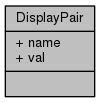
\includegraphics[width=147pt]{dd/d6a/structDisplayPair__coll__graph}
\end{center}
\end{figure}
\subsection*{Data Fields}
\begin{DoxyCompactItemize}
\item 
char $\ast$ \hyperlink{structDisplayPair_a68cc65bc310b262e70eb42b1ecdc2e2d}{name}\hypertarget{structDisplayPair_a68cc65bc310b262e70eb42b1ecdc2e2d}{}\label{structDisplayPair_a68cc65bc310b262e70eb42b1ecdc2e2d}

\begin{DoxyCompactList}\small\item\em Name of the pair. \end{DoxyCompactList}\item 
int $\ast$ \hyperlink{structDisplayPair_abf7b6c359eea9f363705d4c2c8a13ddc}{val}\hypertarget{structDisplayPair_abf7b6c359eea9f363705d4c2c8a13ddc}{}\label{structDisplayPair_abf7b6c359eea9f363705d4c2c8a13ddc}

\begin{DoxyCompactList}\small\item\em Auto updating integer. \end{DoxyCompactList}\end{DoxyCompactItemize}


\subsection{Detailed Description}
Used to display a pair of string and integer auto updating pairs at the top of the screen. 

The documentation for this struct was generated from the following file\+:\begin{DoxyCompactItemize}
\item 
mylib/\hyperlink{s4396122__os__print_8h}{s4396122\+\_\+os\+\_\+print.\+h}\end{DoxyCompactItemize}

\hypertarget{structDrawChar}{}\section{Draw\+Char Struct Reference}
\label{structDrawChar}\index{Draw\+Char@{Draw\+Char}}


Used to store information about a display character.  




{\ttfamily \#include $<$s4396122\+\_\+os\+\_\+draw.\+h$>$}



Collaboration diagram for Draw\+Char\+:\nopagebreak
\begin{figure}[H]
\begin{center}
\leavevmode
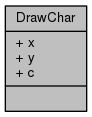
\includegraphics[width=141pt]{d1/d19/structDrawChar__coll__graph}
\end{center}
\end{figure}
\subsection*{Data Fields}
\begin{DoxyCompactItemize}
\item 
int \hyperlink{structDrawChar_adc9ce5763c5a78e7b6e524bfacbb3bc9}{x}\hypertarget{structDrawChar_adc9ce5763c5a78e7b6e524bfacbb3bc9}{}\label{structDrawChar_adc9ce5763c5a78e7b6e524bfacbb3bc9}

\begin{DoxyCompactList}\small\item\em Top left x coord. \end{DoxyCompactList}\item 
int \hyperlink{structDrawChar_a49c68b3c5623c02c534bcd9fed6eec52}{y}\hypertarget{structDrawChar_a49c68b3c5623c02c534bcd9fed6eec52}{}\label{structDrawChar_a49c68b3c5623c02c534bcd9fed6eec52}

\begin{DoxyCompactList}\small\item\em Top left y coord. \end{DoxyCompactList}\item 
int \hyperlink{structDrawChar_ae987c60819064d44007ab101a71d2cd6}{c}\hypertarget{structDrawChar_ae987c60819064d44007ab101a71d2cd6}{}\label{structDrawChar_ae987c60819064d44007ab101a71d2cd6}

\begin{DoxyCompactList}\small\item\em Segment encoded data. \end{DoxyCompactList}\end{DoxyCompactItemize}


\subsection{Detailed Description}
Used to store information about a display character. 

The documentation for this struct was generated from the following file\+:\begin{DoxyCompactItemize}
\item 
mylib/\hyperlink{s4396122__os__draw_8h}{s4396122\+\_\+os\+\_\+draw.\+h}\end{DoxyCompactItemize}

\hypertarget{structDrawCmd}{}\section{Draw\+Cmd Struct Reference}
\label{structDrawCmd}\index{Draw\+Cmd@{Draw\+Cmd}}


A general draw command that can be either character or polygon.  




{\ttfamily \#include $<$s4396122\+\_\+os\+\_\+draw.\+h$>$}



Collaboration diagram for Draw\+Cmd\+:\nopagebreak
\begin{figure}[H]
\begin{center}
\leavevmode
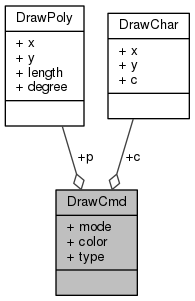
\includegraphics[width=218pt]{dd/d5b/structDrawCmd__coll__graph}
\end{center}
\end{figure}
\subsection*{Data Fields}
\begin{DoxyCompactItemize}
\item 
int \hyperlink{structDrawCmd_a5cf8d6495b68a470cd6ce309c3940776}{mode}\hypertarget{structDrawCmd_a5cf8d6495b68a470cd6ce309c3940776}{}\label{structDrawCmd_a5cf8d6495b68a470cd6ce309c3940776}

\begin{DoxyCompactList}\small\item\em Mode switch to decide if poly or char. \end{DoxyCompactList}\item 
struct \hyperlink{structDrawChar}{Draw\+Char} \hyperlink{structDrawCmd_aaf01f346c2f60c6b269793bfc7d2b636}{c}\hypertarget{structDrawCmd_aaf01f346c2f60c6b269793bfc7d2b636}{}\label{structDrawCmd_aaf01f346c2f60c6b269793bfc7d2b636}

\begin{DoxyCompactList}\small\item\em If char then this contains all the required data. \end{DoxyCompactList}\item 
struct \hyperlink{structDrawPoly}{Draw\+Poly} \hyperlink{structDrawCmd_a0c6659b08b04117b81702addfa7ff9b3}{p}\hypertarget{structDrawCmd_a0c6659b08b04117b81702addfa7ff9b3}{}\label{structDrawCmd_a0c6659b08b04117b81702addfa7ff9b3}

\begin{DoxyCompactList}\small\item\em If poly then this contains all the required data. \end{DoxyCompactList}\item 
enum \hyperlink{s4396122__os__draw_8h_a5fbae3ca85fb9acf7a146955bc6b69c4}{Mouse\+Color} \hyperlink{structDrawCmd_ab07f8653fee749d7bf4d4a5ae10162a5}{color}\hypertarget{structDrawCmd_ab07f8653fee749d7bf4d4a5ae10162a5}{}\label{structDrawCmd_ab07f8653fee749d7bf4d4a5ae10162a5}

\begin{DoxyCompactList}\small\item\em Contains the colour for object. \end{DoxyCompactList}\item 
enum \hyperlink{s4396122__os__draw_8h_a1a15f1712ba14a6877038ffe9c6f7708}{Mouse\+Type} \hyperlink{structDrawCmd_a504719fb9ab8d366ee292d175f04abaf}{type}\hypertarget{structDrawCmd_a504719fb9ab8d366ee292d175f04abaf}{}\label{structDrawCmd_a504719fb9ab8d366ee292d175f04abaf}

\begin{DoxyCompactList}\small\item\em Contains the type for the object. \end{DoxyCompactList}\end{DoxyCompactItemize}


\subsection{Detailed Description}
A general draw command that can be either character or polygon. 

The documentation for this struct was generated from the following file\+:\begin{DoxyCompactItemize}
\item 
mylib/\hyperlink{s4396122__os__draw_8h}{s4396122\+\_\+os\+\_\+draw.\+h}\end{DoxyCompactItemize}

\hypertarget{structDrawPoly}{}\section{Draw\+Poly Struct Reference}
\label{structDrawPoly}\index{Draw\+Poly@{Draw\+Poly}}


Used to store information about a display polygon.  




{\ttfamily \#include $<$s4396122\+\_\+os\+\_\+draw.\+h$>$}



Collaboration diagram for Draw\+Poly\+:\nopagebreak
\begin{figure}[H]
\begin{center}
\leavevmode
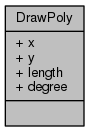
\includegraphics[width=139pt]{d5/df0/structDrawPoly__coll__graph}
\end{center}
\end{figure}
\subsection*{Data Fields}
\begin{DoxyCompactItemize}
\item 
int \hyperlink{structDrawPoly_abaa264798080d3c1064af0028a4705d6}{x}\hypertarget{structDrawPoly_abaa264798080d3c1064af0028a4705d6}{}\label{structDrawPoly_abaa264798080d3c1064af0028a4705d6}

\begin{DoxyCompactList}\small\item\em Top left x coord. \end{DoxyCompactList}\item 
int \hyperlink{structDrawPoly_a1693518092db72ae62079ba775f73275}{y}\hypertarget{structDrawPoly_a1693518092db72ae62079ba775f73275}{}\label{structDrawPoly_a1693518092db72ae62079ba775f73275}

\begin{DoxyCompactList}\small\item\em Top left y coord. \end{DoxyCompactList}\item 
int \hyperlink{structDrawPoly_ae1c2832fdce510858ef0effeb416fc04}{length}\hypertarget{structDrawPoly_ae1c2832fdce510858ef0effeb416fc04}{}\label{structDrawPoly_ae1c2832fdce510858ef0effeb416fc04}

\begin{DoxyCompactList}\small\item\em Length of single polygon side. \end{DoxyCompactList}\item 
int \hyperlink{structDrawPoly_aeebb1111db54f44bb95338c2bde212cd}{degree}\hypertarget{structDrawPoly_aeebb1111db54f44bb95338c2bde212cd}{}\label{structDrawPoly_aeebb1111db54f44bb95338c2bde212cd}

\begin{DoxyCompactList}\small\item\em Number of side to the polygon. \end{DoxyCompactList}\end{DoxyCompactItemize}


\subsection{Detailed Description}
Used to store information about a display polygon. 

The documentation for this struct was generated from the following file\+:\begin{DoxyCompactItemize}
\item 
mylib/\hyperlink{s4396122__os__draw_8h}{s4396122\+\_\+os\+\_\+draw.\+h}\end{DoxyCompactItemize}

\hypertarget{structfuncPair}{}\section{func\+Pair Struct Reference}
\label{structfuncPair}\index{func\+Pair@{func\+Pair}}


Used to pair up a function to an interval.  




{\ttfamily \#include $<$s4396122\+\_\+util\+\_\+func\+\_\+queue.\+h$>$}



Collaboration diagram for func\+Pair\+:\nopagebreak
\begin{figure}[H]
\begin{center}
\leavevmode
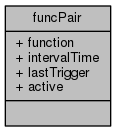
\includegraphics[width=159pt]{d1/d08/structfuncPair__coll__graph}
\end{center}
\end{figure}
\subsection*{Data Fields}
\begin{DoxyCompactItemize}
\item 
void($\ast$ \hyperlink{structfuncPair_a45428448903165e15b2c8e36fc1b5eda}{function} )(void)\hypertarget{structfuncPair_a45428448903165e15b2c8e36fc1b5eda}{}\label{structfuncPair_a45428448903165e15b2c8e36fc1b5eda}

\begin{DoxyCompactList}\small\item\em Function to be called. \end{DoxyCompactList}\item 
int \hyperlink{structfuncPair_a6ffa932fa7c4c28ab86b4d8d88534caa}{interval\+Time}\hypertarget{structfuncPair_a6ffa932fa7c4c28ab86b4d8d88534caa}{}\label{structfuncPair_a6ffa932fa7c4c28ab86b4d8d88534caa}

\begin{DoxyCompactList}\small\item\em Interval to call function on. \end{DoxyCompactList}\item 
unsigned int \hyperlink{structfuncPair_af384061348a84871684a027a4f407a43}{last\+Trigger}\hypertarget{structfuncPair_af384061348a84871684a027a4f407a43}{}\label{structfuncPair_af384061348a84871684a027a4f407a43}

\begin{DoxyCompactList}\small\item\em Time it was last triggered. \end{DoxyCompactList}\item 
int \hyperlink{structfuncPair_a94ea97cd0c02cf5204435a2666abb93b}{active}\hypertarget{structfuncPair_a94ea97cd0c02cf5204435a2666abb93b}{}\label{structfuncPair_a94ea97cd0c02cf5204435a2666abb93b}

\begin{DoxyCompactList}\small\item\em If the current element is active. \end{DoxyCompactList}\end{DoxyCompactItemize}


\subsection{Detailed Description}
Used to pair up a function to an interval. 

The documentation for this struct was generated from the following file\+:\begin{DoxyCompactItemize}
\item 
mylib/\hyperlink{s4396122__util__func__queue_8h}{s4396122\+\_\+util\+\_\+func\+\_\+queue.\+h}\end{DoxyCompactItemize}

\hypertarget{structFuncQueue}{}\section{Func\+Queue Struct Reference}
\label{structFuncQueue}\index{Func\+Queue@{Func\+Queue}}


A struct containing all the required \hyperlink{structFuncQueue}{Func\+Queue} info.  




{\ttfamily \#include $<$s4396122\+\_\+util\+\_\+func\+\_\+queue.\+h$>$}



Collaboration diagram for Func\+Queue\+:\nopagebreak
\begin{figure}[H]
\begin{center}
\leavevmode
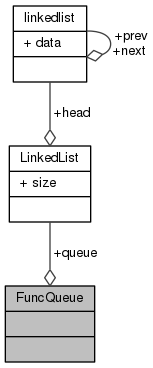
\includegraphics[width=187pt]{d8/dec/structFuncQueue__coll__graph}
\end{center}
\end{figure}
\subsection*{Data Fields}
\begin{DoxyCompactItemize}
\item 
\hyperlink{structLinkedList}{Linked\+List} $\ast$ \hyperlink{structFuncQueue_acb6e930c69d3c30707b39f49670bf490}{queue}\hypertarget{structFuncQueue_acb6e930c69d3c30707b39f49670bf490}{}\label{structFuncQueue_acb6e930c69d3c30707b39f49670bf490}

\begin{DoxyCompactList}\small\item\em \hyperlink{structLinkedList}{Linked\+List} of all the func\+Pairs. \end{DoxyCompactList}\end{DoxyCompactItemize}


\subsection{Detailed Description}
A struct containing all the required \hyperlink{structFuncQueue}{Func\+Queue} info. 

The documentation for this struct was generated from the following file\+:\begin{DoxyCompactItemize}
\item 
mylib/\hyperlink{s4396122__util__func__queue_8h}{s4396122\+\_\+util\+\_\+func\+\_\+queue.\+h}\end{DoxyCompactItemize}

\hypertarget{structintQueue}{}\section{int\+Queue Struct Reference}
\label{structintQueue}\index{int\+Queue@{int\+Queue}}


Individual \hyperlink{structIntQueue}{Int\+Queue} element.  




{\ttfamily \#include $<$s4396122\+\_\+util\+\_\+int\+\_\+queue.\+h$>$}



Collaboration diagram for int\+Queue\+:\nopagebreak
\begin{figure}[H]
\begin{center}
\leavevmode
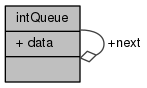
\includegraphics[width=182pt]{db/df4/structintQueue__coll__graph}
\end{center}
\end{figure}
\subsection*{Data Fields}
\begin{DoxyCompactItemize}
\item 
struct \hyperlink{structintQueue}{int\+Queue} $\ast$ \hyperlink{structintQueue_a1702e8e91ebfca0b620791684046fff6}{next}\hypertarget{structintQueue_a1702e8e91ebfca0b620791684046fff6}{}\label{structintQueue_a1702e8e91ebfca0b620791684046fff6}

\begin{DoxyCompactList}\small\item\em Pointer to the next \hyperlink{structintQueue}{int\+Queue} in the \hyperlink{structQueue}{Queue}. \end{DoxyCompactList}\item 
int \hyperlink{structintQueue_a0d3aac3e8322327a2af544acf7986351}{data}\hypertarget{structintQueue_a0d3aac3e8322327a2af544acf7986351}{}\label{structintQueue_a0d3aac3e8322327a2af544acf7986351}

\begin{DoxyCompactList}\small\item\em data stored at current position \end{DoxyCompactList}\end{DoxyCompactItemize}


\subsection{Detailed Description}
Individual \hyperlink{structIntQueue}{Int\+Queue} element. 

The documentation for this struct was generated from the following file\+:\begin{DoxyCompactItemize}
\item 
mylib/\hyperlink{s4396122__util__int__queue_8h}{s4396122\+\_\+util\+\_\+int\+\_\+queue.\+h}\end{DoxyCompactItemize}

\hypertarget{structIntQueue}{}\section{Int\+Queue Struct Reference}
\label{structIntQueue}\index{Int\+Queue@{Int\+Queue}}


The overall \hyperlink{structIntQueue}{Int\+Queue} structure.  




{\ttfamily \#include $<$s4396122\+\_\+util\+\_\+int\+\_\+queue.\+h$>$}



Collaboration diagram for Int\+Queue\+:\nopagebreak
\begin{figure}[H]
\begin{center}
\leavevmode
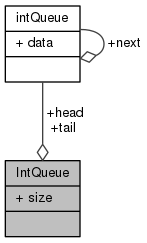
\includegraphics[width=182pt]{dc/de8/structIntQueue__coll__graph}
\end{center}
\end{figure}
\subsection*{Data Fields}
\begin{DoxyCompactItemize}
\item 
struct \hyperlink{structintQueue}{int\+Queue} $\ast$ \hyperlink{structIntQueue_ad10186fedb5ed17c0e225f9ceeb24c04}{head}\hypertarget{structIntQueue_ad10186fedb5ed17c0e225f9ceeb24c04}{}\label{structIntQueue_ad10186fedb5ed17c0e225f9ceeb24c04}

\begin{DoxyCompactList}\small\item\em Pointer to the head of the \hyperlink{structIntQueue}{Int\+Queue}. \end{DoxyCompactList}\item 
struct \hyperlink{structintQueue}{int\+Queue} $\ast$ \hyperlink{structIntQueue_aed5a99ff57f509c35952f0a3499aa77e}{tail}\hypertarget{structIntQueue_aed5a99ff57f509c35952f0a3499aa77e}{}\label{structIntQueue_aed5a99ff57f509c35952f0a3499aa77e}

\begin{DoxyCompactList}\small\item\em Pointer to the tail of the \hyperlink{structIntQueue}{Int\+Queue}. \end{DoxyCompactList}\item 
int \hyperlink{structIntQueue_a723612c1e494877450388082f5b65fc4}{size}\hypertarget{structIntQueue_a723612c1e494877450388082f5b65fc4}{}\label{structIntQueue_a723612c1e494877450388082f5b65fc4}

\begin{DoxyCompactList}\small\item\em Size of the \hyperlink{structIntQueue}{Int\+Queue}. \end{DoxyCompactList}\end{DoxyCompactItemize}


\subsection{Detailed Description}
The overall \hyperlink{structIntQueue}{Int\+Queue} structure. 

The documentation for this struct was generated from the following file\+:\begin{DoxyCompactItemize}
\item 
mylib/\hyperlink{s4396122__util__int__queue_8h}{s4396122\+\_\+util\+\_\+int\+\_\+queue.\+h}\end{DoxyCompactItemize}

\hypertarget{structLinkedList}{}\section{Linked\+List Struct Reference}
\label{structLinkedList}\index{Linked\+List@{Linked\+List}}


Structure containing all the information needed for a linkedlist.  




{\ttfamily \#include $<$s4396122\+\_\+util\+\_\+linkedlist.\+h$>$}



Collaboration diagram for Linked\+List\+:\nopagebreak
\begin{figure}[H]
\begin{center}
\leavevmode
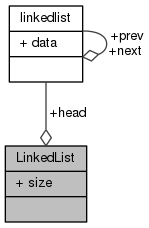
\includegraphics[width=184pt]{d5/d04/structLinkedList__coll__graph}
\end{center}
\end{figure}
\subsection*{Data Fields}
\begin{DoxyCompactItemize}
\item 
struct \hyperlink{structlinkedlist}{linkedlist} $\ast$ \hyperlink{structLinkedList_ad0529bfec20bc43e95bb68a8bb8bf1a1}{head}\hypertarget{structLinkedList_ad0529bfec20bc43e95bb68a8bb8bf1a1}{}\label{structLinkedList_ad0529bfec20bc43e95bb68a8bb8bf1a1}

\begin{DoxyCompactList}\small\item\em Pointer to the head to the list. \end{DoxyCompactList}\item 
int \hyperlink{structLinkedList_ad84541a559b15c98b3171c5d24ad90ef}{size}\hypertarget{structLinkedList_ad84541a559b15c98b3171c5d24ad90ef}{}\label{structLinkedList_ad84541a559b15c98b3171c5d24ad90ef}

\begin{DoxyCompactList}\small\item\em Size of the list. \end{DoxyCompactList}\end{DoxyCompactItemize}


\subsection{Detailed Description}
Structure containing all the information needed for a linkedlist. 

The documentation for this struct was generated from the following file\+:\begin{DoxyCompactItemize}
\item 
mylib/\hyperlink{s4396122__util__linkedlist_8h}{s4396122\+\_\+util\+\_\+linkedlist.\+h}\end{DoxyCompactItemize}

\hypertarget{structlinkedlist}{}\section{linkedlist Struct Reference}
\label{structlinkedlist}\index{linkedlist@{linkedlist}}


A linkedlist element.  




{\ttfamily \#include $<$s4396122\+\_\+util\+\_\+linkedlist.\+h$>$}



Collaboration diagram for linkedlist\+:\nopagebreak
\begin{figure}[H]
\begin{center}
\leavevmode
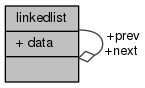
\includegraphics[width=181pt]{d3/d66/structlinkedlist__coll__graph}
\end{center}
\end{figure}
\subsection*{Data Fields}
\begin{DoxyCompactItemize}
\item 
struct \hyperlink{structlinkedlist}{linkedlist} $\ast$ \hyperlink{structlinkedlist_acfe28edfbfca94248d2552a19efbd2a6}{prev}\hypertarget{structlinkedlist_acfe28edfbfca94248d2552a19efbd2a6}{}\label{structlinkedlist_acfe28edfbfca94248d2552a19efbd2a6}

\begin{DoxyCompactList}\small\item\em Pointer to the prev element in the array. \end{DoxyCompactList}\item 
struct \hyperlink{structlinkedlist}{linkedlist} $\ast$ \hyperlink{structlinkedlist_a1cd8b31b9e357b1b2b4b862eeca6863c}{next}\hypertarget{structlinkedlist_a1cd8b31b9e357b1b2b4b862eeca6863c}{}\label{structlinkedlist_a1cd8b31b9e357b1b2b4b862eeca6863c}

\begin{DoxyCompactList}\small\item\em Pointer to the next element in the array. \end{DoxyCompactList}\item 
void $\ast$ \hyperlink{structlinkedlist_aa70dbbff6bbb175200391df764e46d1c}{data}\hypertarget{structlinkedlist_aa70dbbff6bbb175200391df764e46d1c}{}\label{structlinkedlist_aa70dbbff6bbb175200391df764e46d1c}

\begin{DoxyCompactList}\small\item\em Pointer to the data being stored. \end{DoxyCompactList}\end{DoxyCompactItemize}


\subsection{Detailed Description}
A linkedlist element. 

The documentation for this struct was generated from the following file\+:\begin{DoxyCompactItemize}
\item 
mylib/\hyperlink{s4396122__util__linkedlist_8h}{s4396122\+\_\+util\+\_\+linkedlist.\+h}\end{DoxyCompactItemize}

\hypertarget{structMap}{}\section{Map Struct Reference}
\label{structMap}\index{Map@{Map}}


Structure containing all the information for the \hyperlink{structMap}{Map}.  




{\ttfamily \#include $<$s4396122\+\_\+util\+\_\+map.\+h$>$}



Collaboration diagram for Map\+:\nopagebreak
\begin{figure}[H]
\begin{center}
\leavevmode
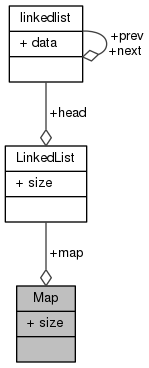
\includegraphics[width=184pt]{d7/d16/structMap__coll__graph}
\end{center}
\end{figure}
\subsection*{Data Fields}
\begin{DoxyCompactItemize}
\item 
\hyperlink{structLinkedList}{Linked\+List} $\ast$$\ast$ \hyperlink{structMap_ace4bbefe0154f313258c4d68b8bcc500}{map}\hypertarget{structMap_ace4bbefe0154f313258c4d68b8bcc500}{}\label{structMap_ace4bbefe0154f313258c4d68b8bcc500}

\begin{DoxyCompactList}\small\item\em An array of Linked\+Lists of width M\+A\+P\+\_\+\+S\+I\+ZE. \end{DoxyCompactList}\item 
int \hyperlink{structMap_ae00b1f478d27d81e4274788ef0b4f7af}{size}\hypertarget{structMap_ae00b1f478d27d81e4274788ef0b4f7af}{}\label{structMap_ae00b1f478d27d81e4274788ef0b4f7af}

\begin{DoxyCompactList}\small\item\em Size of the map. \end{DoxyCompactList}\end{DoxyCompactItemize}


\subsection{Detailed Description}
Structure containing all the information for the \hyperlink{structMap}{Map}. 

The documentation for this struct was generated from the following file\+:\begin{DoxyCompactItemize}
\item 
mylib/\hyperlink{s4396122__util__map_8h}{s4396122\+\_\+util\+\_\+map.\+h}\end{DoxyCompactItemize}

\hypertarget{structMapPair}{}\section{Map\+Pair Struct Reference}
\label{structMapPair}\index{Map\+Pair@{Map\+Pair}}


A single pair element of the map.  




{\ttfamily \#include $<$s4396122\+\_\+util\+\_\+map.\+h$>$}



Collaboration diagram for Map\+Pair\+:\nopagebreak
\begin{figure}[H]
\begin{center}
\leavevmode
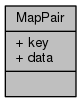
\includegraphics[width=133pt]{d8/d36/structMapPair__coll__graph}
\end{center}
\end{figure}
\subsection*{Data Fields}
\begin{DoxyCompactItemize}
\item 
int \hyperlink{structMapPair_af53f875c2b8789ce00a2bf6afb62fa6f}{key}\hypertarget{structMapPair_af53f875c2b8789ce00a2bf6afb62fa6f}{}\label{structMapPair_af53f875c2b8789ce00a2bf6afb62fa6f}

\begin{DoxyCompactList}\small\item\em The integer representation of the key. \end{DoxyCompactList}\item 
void $\ast$ \hyperlink{structMapPair_a7fb84ba610f72b02859dee69a52b42d1}{data}\hypertarget{structMapPair_a7fb84ba610f72b02859dee69a52b42d1}{}\label{structMapPair_a7fb84ba610f72b02859dee69a52b42d1}

\begin{DoxyCompactList}\small\item\em The data associated with the key. \end{DoxyCompactList}\end{DoxyCompactItemize}


\subsection{Detailed Description}
A single pair element of the map. 

The documentation for this struct was generated from the following file\+:\begin{DoxyCompactItemize}
\item 
mylib/\hyperlink{s4396122__util__map_8h}{s4396122\+\_\+util\+\_\+map.\+h}\end{DoxyCompactItemize}

\hypertarget{structMatrix}{}\section{Matrix Struct Reference}
\label{structMatrix}\index{Matrix@{Matrix}}


Structure containing all the information required for a \hyperlink{structMatrix}{Matrix}.  




{\ttfamily \#include $<$s4396122\+\_\+util\+\_\+matrix.\+h$>$}



Collaboration diagram for Matrix\+:\nopagebreak
\begin{figure}[H]
\begin{center}
\leavevmode
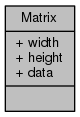
\includegraphics[width=132pt]{d6/d98/structMatrix__coll__graph}
\end{center}
\end{figure}
\subsection*{Data Fields}
\begin{DoxyCompactItemize}
\item 
int \hyperlink{structMatrix_ad4320bd2dc03fd11887d3ba350c6c8ef}{width}\hypertarget{structMatrix_ad4320bd2dc03fd11887d3ba350c6c8ef}{}\label{structMatrix_ad4320bd2dc03fd11887d3ba350c6c8ef}

\begin{DoxyCompactList}\small\item\em Width of the \hyperlink{structMatrix}{Matrix}. \end{DoxyCompactList}\item 
int \hyperlink{structMatrix_a0b5614256a04ece0ea54b8aad7e6980c}{height}\hypertarget{structMatrix_a0b5614256a04ece0ea54b8aad7e6980c}{}\label{structMatrix_a0b5614256a04ece0ea54b8aad7e6980c}

\begin{DoxyCompactList}\small\item\em Height of the \hyperlink{structMatrix}{Matrix}. \end{DoxyCompactList}\item 
int $\ast$$\ast$ \hyperlink{structMatrix_afda04dbb307a169b4235dba98fb5b9df}{data}\hypertarget{structMatrix_afda04dbb307a169b4235dba98fb5b9df}{}\label{structMatrix_afda04dbb307a169b4235dba98fb5b9df}

\begin{DoxyCompactList}\small\item\em Data contained within the \hyperlink{structMatrix}{Matrix}. \end{DoxyCompactList}\end{DoxyCompactItemize}


\subsection{Detailed Description}
Structure containing all the information required for a \hyperlink{structMatrix}{Matrix}. 

The documentation for this struct was generated from the following file\+:\begin{DoxyCompactItemize}
\item 
mylib/\hyperlink{s4396122__util__matrix_8h}{s4396122\+\_\+util\+\_\+matrix.\+h}\end{DoxyCompactItemize}

\hypertarget{structMouseCommand}{}\section{Mouse\+Command Struct Reference}
\label{structMouseCommand}\index{Mouse\+Command@{Mouse\+Command}}


Simple mouse command struct used for basic things like mouse movement and mouse buttons.  




{\ttfamily \#include $<$s4396122\+\_\+os\+\_\+draw.\+h$>$}



Collaboration diagram for Mouse\+Command\+:\nopagebreak
\begin{figure}[H]
\begin{center}
\leavevmode
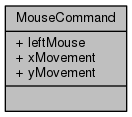
\includegraphics[width=171pt]{db/ded/structMouseCommand__coll__graph}
\end{center}
\end{figure}
\subsection*{Data Fields}
\begin{DoxyCompactItemize}
\item 
int \hyperlink{structMouseCommand_afef1023fdb35d2320a6fe785ac391d33}{left\+Mouse}\hypertarget{structMouseCommand_afef1023fdb35d2320a6fe785ac391d33}{}\label{structMouseCommand_afef1023fdb35d2320a6fe785ac391d33}

\begin{DoxyCompactList}\small\item\em If the left mouse button is down or not. \end{DoxyCompactList}\item 
int \hyperlink{structMouseCommand_ab6f61004ed3bf7be2db14871ea2e5d45}{x\+Movement}\hypertarget{structMouseCommand_ab6f61004ed3bf7be2db14871ea2e5d45}{}\label{structMouseCommand_ab6f61004ed3bf7be2db14871ea2e5d45}

\begin{DoxyCompactList}\small\item\em X mouse coord. \end{DoxyCompactList}\item 
int \hyperlink{structMouseCommand_aece464c7fd066912b6bd0d08ba825a64}{y\+Movement}\hypertarget{structMouseCommand_aece464c7fd066912b6bd0d08ba825a64}{}\label{structMouseCommand_aece464c7fd066912b6bd0d08ba825a64}

\begin{DoxyCompactList}\small\item\em Y mouse coord. \end{DoxyCompactList}\end{DoxyCompactItemize}


\subsection{Detailed Description}
Simple mouse command struct used for basic things like mouse movement and mouse buttons. 

The documentation for this struct was generated from the following file\+:\begin{DoxyCompactItemize}
\item 
mylib/\hyperlink{s4396122__os__draw_8h}{s4396122\+\_\+os\+\_\+draw.\+h}\end{DoxyCompactItemize}

\hypertarget{structPanTiltMessage}{}\section{Pan\+Tilt\+Message Struct Reference}
\label{structPanTiltMessage}\index{Pan\+Tilt\+Message@{Pan\+Tilt\+Message}}


Used to store a pantilt command.  




{\ttfamily \#include $<$s4396122\+\_\+os\+\_\+pantilt.\+h$>$}



Collaboration diagram for Pan\+Tilt\+Message\+:\nopagebreak
\begin{figure}[H]
\begin{center}
\leavevmode
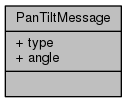
\includegraphics[width=167pt]{d2/d3e/structPanTiltMessage__coll__graph}
\end{center}
\end{figure}
\subsection*{Data Fields}
\begin{DoxyCompactItemize}
\item 
char \hyperlink{structPanTiltMessage_af6ace5a01a0088c36fd6caf0aef1fd6d}{type}\hypertarget{structPanTiltMessage_af6ace5a01a0088c36fd6caf0aef1fd6d}{}\label{structPanTiltMessage_af6ace5a01a0088c36fd6caf0aef1fd6d}

\begin{DoxyCompactList}\small\item\em Whether the angle applies to Pan or Tilt. \end{DoxyCompactList}\item 
signed short \hyperlink{structPanTiltMessage_a01e22a313f9fd0585ab72af8f54b4014}{angle}\hypertarget{structPanTiltMessage_a01e22a313f9fd0585ab72af8f54b4014}{}\label{structPanTiltMessage_a01e22a313f9fd0585ab72af8f54b4014}

\begin{DoxyCompactList}\small\item\em Then angle to move. \end{DoxyCompactList}\end{DoxyCompactItemize}


\subsection{Detailed Description}
Used to store a pantilt command. 

The documentation for this struct was generated from the following file\+:\begin{DoxyCompactItemize}
\item 
mylib/\hyperlink{s4396122__os__pantilt_8h}{s4396122\+\_\+os\+\_\+pantilt.\+h}\end{DoxyCompactItemize}

\hypertarget{structPortLand}{}\section{Port\+Land Struct Reference}
\label{structPortLand}\index{Port\+Land@{Port\+Land}}


structure for containing the result of the pl register of the accelerometer  




{\ttfamily \#include $<$s4396122\+\_\+hal\+\_\+accel.\+h$>$}



Collaboration diagram for Port\+Land\+:\nopagebreak
\begin{figure}[H]
\begin{center}
\leavevmode
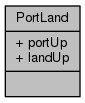
\includegraphics[width=136pt]{d4/d31/structPortLand__coll__graph}
\end{center}
\end{figure}
\subsection*{Data Fields}
\begin{DoxyCompactItemize}
\item 
int \hyperlink{structPortLand_a7c3278bf797bd36358b3a3037d80e243}{port\+Up}\hypertarget{structPortLand_a7c3278bf797bd36358b3a3037d80e243}{}\label{structPortLand_a7c3278bf797bd36358b3a3037d80e243}

\begin{DoxyCompactList}\small\item\em The value of the portrait bit. \end{DoxyCompactList}\item 
int \hyperlink{structPortLand_aad6cbd74cd584b602411b466fa87c2ce}{land\+Up}\hypertarget{structPortLand_aad6cbd74cd584b602411b466fa87c2ce}{}\label{structPortLand_aad6cbd74cd584b602411b466fa87c2ce}

\begin{DoxyCompactList}\small\item\em The value of the landscape bit. \end{DoxyCompactList}\end{DoxyCompactItemize}


\subsection{Detailed Description}
structure for containing the result of the pl register of the accelerometer 

The documentation for this struct was generated from the following file\+:\begin{DoxyCompactItemize}
\item 
mylib/\hyperlink{s4396122__hal__accel_8h}{s4396122\+\_\+hal\+\_\+accel.\+h}\end{DoxyCompactItemize}

\hypertarget{structQueue}{}\section{Queue Struct Reference}
\label{structQueue}\index{Queue@{Queue}}


Structure of all the information required for a \hyperlink{structQueue}{Queue}.  




{\ttfamily \#include $<$s4396122\+\_\+util\+\_\+queue.\+h$>$}



Collaboration diagram for Queue\+:\nopagebreak
\begin{figure}[H]
\begin{center}
\leavevmode
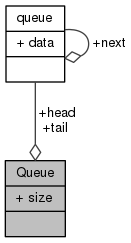
\includegraphics[width=171pt]{d1/dec/structQueue__coll__graph}
\end{center}
\end{figure}
\subsection*{Data Fields}
\begin{DoxyCompactItemize}
\item 
struct \hyperlink{structqueue}{queue} $\ast$ \hyperlink{structQueue_a64cfeab728b5d35d15859a6441ef0a35}{head}\hypertarget{structQueue_a64cfeab728b5d35d15859a6441ef0a35}{}\label{structQueue_a64cfeab728b5d35d15859a6441ef0a35}

\begin{DoxyCompactList}\small\item\em Pointer to the head of the \hyperlink{structQueue}{Queue}. \end{DoxyCompactList}\item 
struct \hyperlink{structqueue}{queue} $\ast$ \hyperlink{structQueue_a3c273fad6555af394c06265aca0c6270}{tail}\hypertarget{structQueue_a3c273fad6555af394c06265aca0c6270}{}\label{structQueue_a3c273fad6555af394c06265aca0c6270}

\begin{DoxyCompactList}\small\item\em Pointer to the tail of the \hyperlink{structQueue}{Queue}. \end{DoxyCompactList}\item 
int \hyperlink{structQueue_ac7d9701d244e3ba255ef8556e0562dc6}{size}\hypertarget{structQueue_ac7d9701d244e3ba255ef8556e0562dc6}{}\label{structQueue_ac7d9701d244e3ba255ef8556e0562dc6}

\begin{DoxyCompactList}\small\item\em Size of the \hyperlink{structQueue}{Queue}. \end{DoxyCompactList}\end{DoxyCompactItemize}


\subsection{Detailed Description}
Structure of all the information required for a \hyperlink{structQueue}{Queue}. 

The documentation for this struct was generated from the following file\+:\begin{DoxyCompactItemize}
\item 
mylib/\hyperlink{s4396122__util__queue_8h}{s4396122\+\_\+util\+\_\+queue.\+h}\end{DoxyCompactItemize}

\hypertarget{structqueue}{}\section{queue Struct Reference}
\label{structqueue}\index{queue@{queue}}


A single \hyperlink{structQueue}{Queue} element.  




{\ttfamily \#include $<$s4396122\+\_\+util\+\_\+queue.\+h$>$}



Collaboration diagram for queue\+:\nopagebreak
\begin{figure}[H]
\begin{center}
\leavevmode
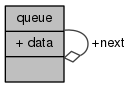
\includegraphics[width=170pt]{dd/d75/structqueue__coll__graph}
\end{center}
\end{figure}
\subsection*{Data Fields}
\begin{DoxyCompactItemize}
\item 
struct \hyperlink{structqueue}{queue} $\ast$ \hyperlink{structqueue_ad9a4d0c0515c80148e0ca26f99ac4feb}{next}\hypertarget{structqueue_ad9a4d0c0515c80148e0ca26f99ac4feb}{}\label{structqueue_ad9a4d0c0515c80148e0ca26f99ac4feb}

\begin{DoxyCompactList}\small\item\em Pointer to the next item in the \hyperlink{structQueue}{Queue}. \end{DoxyCompactList}\item 
void $\ast$ \hyperlink{structqueue_a36d42bcd5973f1c6d1f45df1bc0b209c}{data}\hypertarget{structqueue_a36d42bcd5973f1c6d1f45df1bc0b209c}{}\label{structqueue_a36d42bcd5973f1c6d1f45df1bc0b209c}

\begin{DoxyCompactList}\small\item\em Pointer to the data for this element. \end{DoxyCompactList}\end{DoxyCompactItemize}


\subsection{Detailed Description}
A single \hyperlink{structQueue}{Queue} element. 

The documentation for this struct was generated from the following file\+:\begin{DoxyCompactItemize}
\item 
mylib/\hyperlink{s4396122__util__queue_8h}{s4396122\+\_\+util\+\_\+queue.\+h}\end{DoxyCompactItemize}

\hypertarget{structTaskHolder}{}\section{Task\+Holder Struct Reference}
\label{structTaskHolder}\index{Task\+Holder@{Task\+Holder}}


Struct for holder all the information required to re-\/create a task.  




Collaboration diagram for Task\+Holder\+:\nopagebreak
\begin{figure}[H]
\begin{center}
\leavevmode
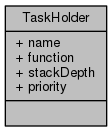
\includegraphics[width=156pt]{d2/dc6/structTaskHolder__coll__graph}
\end{center}
\end{figure}
\subsection*{Data Fields}
\begin{DoxyCompactItemize}
\item 
char $\ast$ \hyperlink{structTaskHolder_a1cd66557649e19026e3ce6fa58fe7725}{name}\hypertarget{structTaskHolder_a1cd66557649e19026e3ce6fa58fe7725}{}\label{structTaskHolder_a1cd66557649e19026e3ce6fa58fe7725}

\begin{DoxyCompactList}\small\item\em Name of the task. \end{DoxyCompactList}\item 
Task\+Function\+\_\+t \hyperlink{structTaskHolder_acabbddfc114b4acdbed43ab321f33cfa}{function}\hypertarget{structTaskHolder_acabbddfc114b4acdbed43ab321f33cfa}{}\label{structTaskHolder_acabbddfc114b4acdbed43ab321f33cfa}

\begin{DoxyCompactList}\small\item\em The function associated with the task. \end{DoxyCompactList}\item 
unsigned short \hyperlink{structTaskHolder_a99ef30650dbf385f948a34d82c3f9519}{stack\+Depth}\hypertarget{structTaskHolder_a99ef30650dbf385f948a34d82c3f9519}{}\label{structTaskHolder_a99ef30650dbf385f948a34d82c3f9519}

\begin{DoxyCompactList}\small\item\em The amount of stack allocated to the task. \end{DoxyCompactList}\item 
U\+Base\+Type\+\_\+t \hyperlink{structTaskHolder_a1fe7561b26de35d8c561e94af3fc20b9}{priority}\hypertarget{structTaskHolder_a1fe7561b26de35d8c561e94af3fc20b9}{}\label{structTaskHolder_a1fe7561b26de35d8c561e94af3fc20b9}

\begin{DoxyCompactList}\small\item\em The task priority. \end{DoxyCompactList}\end{DoxyCompactItemize}


\subsection{Detailed Description}
Struct for holder all the information required to re-\/create a task. 

The documentation for this struct was generated from the following file\+:\begin{DoxyCompactItemize}
\item 
assignment2/\hyperlink{main_8c}{main.\+c}\end{DoxyCompactItemize}

\hypertarget{structtcpConnection}{}\section{tcp\+Connection Struct Reference}
\label{structtcpConnection}\index{tcp\+Connection@{tcp\+Connection}}


Structure containing all the information required for a network connection.  




{\ttfamily \#include $<$s4396122\+\_\+hal\+\_\+tcp.\+h$>$}



Collaboration diagram for tcp\+Connection\+:\nopagebreak
\begin{figure}[H]
\begin{center}
\leavevmode
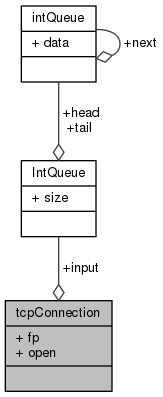
\includegraphics[width=194pt]{d5/d01/structtcpConnection__coll__graph}
\end{center}
\end{figure}
\subsection*{Data Fields}
\begin{DoxyCompactItemize}
\item 
int \hyperlink{structtcpConnection_a7d642c6f8bda4cfa978eb8f4288ee5df}{fp}\hypertarget{structtcpConnection_a7d642c6f8bda4cfa978eb8f4288ee5df}{}\label{structtcpConnection_a7d642c6f8bda4cfa978eb8f4288ee5df}

\begin{DoxyCompactList}\small\item\em File descriptor of the current connection. \end{DoxyCompactList}\item 
\hyperlink{structIntQueue}{Int\+Queue} $\ast$ \hyperlink{structtcpConnection_aad0ac0e1dec718e9cea42852934a315e}{input}\hypertarget{structtcpConnection_aad0ac0e1dec718e9cea42852934a315e}{}\label{structtcpConnection_aad0ac0e1dec718e9cea42852934a315e}

\begin{DoxyCompactList}\small\item\em Integer buffer of the current network input. \end{DoxyCompactList}\item 
int \hyperlink{structtcpConnection_a9597618fdbb9faa5d83d54d8f2126935}{open}\hypertarget{structtcpConnection_a9597618fdbb9faa5d83d54d8f2126935}{}\label{structtcpConnection_a9597618fdbb9faa5d83d54d8f2126935}

\begin{DoxyCompactList}\small\item\em Status of if the network is still open or not. \end{DoxyCompactList}\end{DoxyCompactItemize}


\subsection{Detailed Description}
Structure containing all the information required for a network connection. 

The documentation for this struct was generated from the following file\+:\begin{DoxyCompactItemize}
\item 
mylib/\hyperlink{s4396122__hal__tcp_8h}{s4396122\+\_\+hal\+\_\+tcp.\+h}\end{DoxyCompactItemize}

\chapter{File Documentation}
\hypertarget{main_8c}{}\section{assignment2/main.c File Reference}
\label{main_8c}\index{assignment2/main.\+c@{assignment2/main.\+c}}


Main file for project 2.  


{\ttfamily \#include \char`\"{}Free\+R\+T\+O\+S\+Config.\+h\char`\"{}}\\*
{\ttfamily \#include \char`\"{}board.\+h\char`\"{}}\\*
{\ttfamily \#include $<$stdio.\+h$>$}\\*
{\ttfamily \#include \char`\"{}s4396122\+\_\+hal\+\_\+tcp.\+h\char`\"{}}\\*
{\ttfamily \#include \char`\"{}s4396122\+\_\+os\+\_\+draw.\+h\char`\"{}}\\*
{\ttfamily \#include \char`\"{}s4396122\+\_\+cli\+\_\+draw.\+h\char`\"{}}\\*
{\ttfamily \#include \char`\"{}s4396122\+\_\+hal\+\_\+irremote.\+h\char`\"{}}\\*
{\ttfamily \#include \char`\"{}s4396122\+\_\+hal\+\_\+ir.\+h\char`\"{}}\\*
{\ttfamily \#include \char`\"{}s4396122\+\_\+util\+\_\+map.\+h\char`\"{}}\\*
{\ttfamily \#include \char`\"{}s4396122\+\_\+util\+\_\+int\+\_\+queue.\+h\char`\"{}}\\*
{\ttfamily \#include \char`\"{}s4396122\+\_\+hal\+\_\+joystick.\+h\char`\"{}}\\*
{\ttfamily \#include \char`\"{}s4396122\+\_\+os\+\_\+joystick.\+h\char`\"{}}\\*
{\ttfamily \#include \char`\"{}s4396122\+\_\+cli\+\_\+joystick.\+h\char`\"{}}\\*
{\ttfamily \#include \char`\"{}s4396122\+\_\+hal\+\_\+accel.\+h\char`\"{}}\\*
{\ttfamily \#include \char`\"{}s4396122\+\_\+os\+\_\+mqtt.\+h\char`\"{}}\\*
{\ttfamily \#include \char`\"{}Free\+R\+T\+O\+S.\+h\char`\"{}}\\*
{\ttfamily \#include \char`\"{}task.\+h\char`\"{}}\\*
{\ttfamily \#include \char`\"{}queue.\+h\char`\"{}}\\*
{\ttfamily \#include \char`\"{}Free\+R\+T\+O\+S\+\_\+\+C\+L\+I.\+h\char`\"{}}\\*
Include dependency graph for main.\+c\+:\nopagebreak
\begin{figure}[H]
\begin{center}
\leavevmode
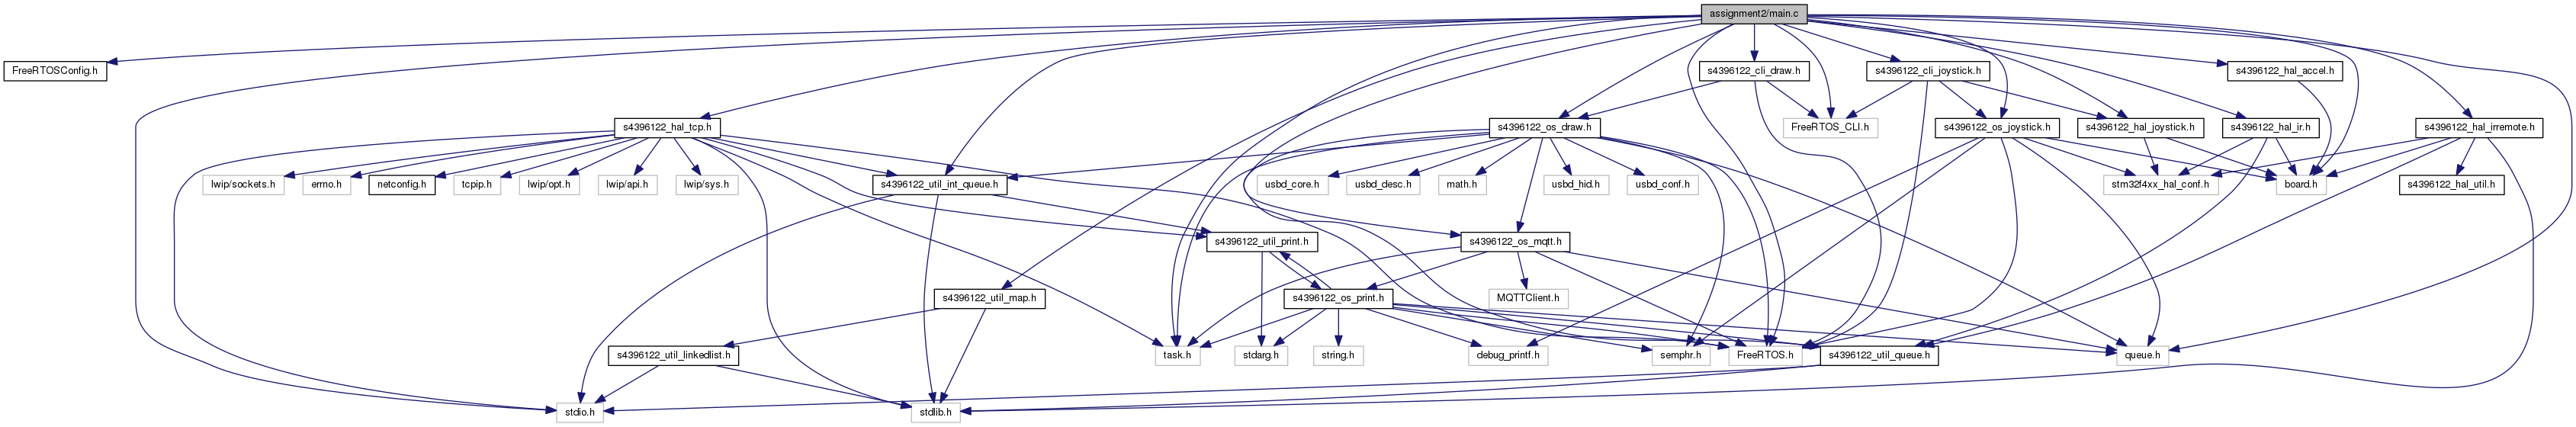
\includegraphics[width=350pt]{d4/d10/main_8c__incl}
\end{center}
\end{figure}
\subsection*{Data Structures}
\begin{DoxyCompactItemize}
\item 
struct \hyperlink{structTaskHolder}{Task\+Holder}
\begin{DoxyCompactList}\small\item\em Struct for holder all the information required to re-\/create a task. \end{DoxyCompactList}\end{DoxyCompactItemize}
\subsection*{Macros}
\begin{DoxyCompactItemize}
\item 
\#define \hyperlink{main_8c_a4fa0dea8934493e58ecab60099247911}{main\+L\+E\+D\+\_\+\+P\+R\+I\+O\+R\+I\+TY}~(tsk\+I\+D\+L\+E\+\_\+\+P\+R\+I\+O\+R\+I\+TY + 4)\hypertarget{main_8c_a4fa0dea8934493e58ecab60099247911}{}\label{main_8c_a4fa0dea8934493e58ecab60099247911}

\begin{DoxyCompactList}\small\item\em Main L\+ED priority. \end{DoxyCompactList}\item 
\#define \hyperlink{main_8c_abea22f101a2ab2988b4daf0d8d14c7c6}{main\+L\+E\+D\+\_\+\+T\+A\+S\+K\+\_\+\+S\+T\+A\+C\+K\+\_\+\+S\+I\+ZE}~(config\+M\+I\+N\+I\+M\+A\+L\+\_\+\+S\+T\+A\+C\+K\+\_\+\+S\+I\+ZE $\ast$ 2)\hypertarget{main_8c_abea22f101a2ab2988b4daf0d8d14c7c6}{}\label{main_8c_abea22f101a2ab2988b4daf0d8d14c7c6}

\begin{DoxyCompactList}\small\item\em Main L\+ED stack size. \end{DoxyCompactList}\item 
\#define \hyperlink{main_8c_a94c5125c6e09fec149dcecb5612f342f}{main\+Task\+\_\+\+P\+R\+I\+O\+R\+I\+TY}~(tsk\+I\+D\+L\+E\+\_\+\+P\+R\+I\+O\+R\+I\+TY + 3)\hypertarget{main_8c_a94c5125c6e09fec149dcecb5612f342f}{}\label{main_8c_a94c5125c6e09fec149dcecb5612f342f}

\begin{DoxyCompactList}\small\item\em Main C\+LI task priority. \end{DoxyCompactList}\item 
\#define \hyperlink{main_8c_ac15a0ecb5846c2e0fba03e6a806bfea4}{main\+Task\+\_\+\+T\+A\+S\+K\+\_\+\+S\+T\+A\+C\+K\+\_\+\+S\+I\+ZE}~(config\+M\+I\+N\+I\+M\+A\+L\+\_\+\+S\+T\+A\+C\+K\+\_\+\+S\+I\+ZE $\ast$ 8)\hypertarget{main_8c_ac15a0ecb5846c2e0fba03e6a806bfea4}{}\label{main_8c_ac15a0ecb5846c2e0fba03e6a806bfea4}

\begin{DoxyCompactList}\small\item\em Main C\+LI task stack size. \end{DoxyCompactList}\item 
\#define \hyperlink{main_8c_abb4deec5ed0637ea3e9da85c9cc6839a}{drawer\+Task\+\_\+\+P\+R\+I\+O\+R\+I\+TY}~(tsk\+I\+D\+L\+E\+\_\+\+P\+R\+I\+O\+R\+I\+TY + 3)\hypertarget{main_8c_abb4deec5ed0637ea3e9da85c9cc6839a}{}\label{main_8c_abb4deec5ed0637ea3e9da85c9cc6839a}

\begin{DoxyCompactList}\small\item\em Drawer task priority. \end{DoxyCompactList}\item 
\#define \hyperlink{main_8c_aa6fe14df4bf785b5075ce702dee35155}{drawer\+Task\+\_\+\+T\+A\+S\+K\+\_\+\+S\+T\+A\+C\+K\+\_\+\+S\+I\+ZE}~(config\+M\+I\+N\+I\+M\+A\+L\+\_\+\+S\+T\+A\+C\+K\+\_\+\+S\+I\+ZE $\ast$ 2)\hypertarget{main_8c_aa6fe14df4bf785b5075ce702dee35155}{}\label{main_8c_aa6fe14df4bf785b5075ce702dee35155}

\begin{DoxyCompactList}\small\item\em Drawer task stack size. \end{DoxyCompactList}\item 
\#define \hyperlink{main_8c_aeb7e6acd99e281e53dadac24c8d3bbc9}{I\+R\+Task\+\_\+\+P\+R\+I\+O\+R\+I\+TY}~(tsk\+I\+D\+L\+E\+\_\+\+P\+R\+I\+O\+R\+I\+TY + 2)\hypertarget{main_8c_aeb7e6acd99e281e53dadac24c8d3bbc9}{}\label{main_8c_aeb7e6acd99e281e53dadac24c8d3bbc9}

\begin{DoxyCompactList}\small\item\em IR task priority. \end{DoxyCompactList}\item 
\#define \hyperlink{main_8c_a2705eaec87619d5effd4fd149c4af5d5}{I\+R\+Task\+\_\+\+T\+A\+S\+K\+\_\+\+S\+T\+A\+C\+K\+\_\+\+S\+I\+ZE}~(config\+M\+I\+N\+I\+M\+A\+L\+\_\+\+S\+T\+A\+C\+K\+\_\+\+S\+I\+ZE $\ast$ 5)\hypertarget{main_8c_a2705eaec87619d5effd4fd149c4af5d5}{}\label{main_8c_a2705eaec87619d5effd4fd149c4af5d5}

\begin{DoxyCompactList}\small\item\em IR task stack size. \end{DoxyCompactList}\item 
\#define \hyperlink{main_8c_a291d62083d42675555973954ff77a7d5}{joystick\+Task\+\_\+\+P\+R\+I\+O\+R\+I\+TY}~(tsk\+I\+D\+L\+E\+\_\+\+P\+R\+I\+O\+R\+I\+TY + 2)\hypertarget{main_8c_a291d62083d42675555973954ff77a7d5}{}\label{main_8c_a291d62083d42675555973954ff77a7d5}

\begin{DoxyCompactList}\small\item\em Joystick priority. \end{DoxyCompactList}\item 
\#define \hyperlink{main_8c_ae8fe6b98f76d8ca6155c766d21de9539}{joystick\+Task\+\_\+\+T\+A\+S\+K\+\_\+\+S\+T\+A\+C\+K\+\_\+\+S\+I\+ZE}~(config\+M\+I\+N\+I\+M\+A\+L\+\_\+\+S\+T\+A\+C\+K\+\_\+\+S\+I\+ZE $\ast$ 5)\hypertarget{main_8c_ae8fe6b98f76d8ca6155c766d21de9539}{}\label{main_8c_ae8fe6b98f76d8ca6155c766d21de9539}

\begin{DoxyCompactList}\small\item\em Joystick task stack size. \end{DoxyCompactList}\item 
\#define \hyperlink{main_8c_a8b935a3aae000c62d138f5cd2cc7af36}{accel\+Task\+\_\+\+P\+R\+I\+O\+R\+I\+TY}~(tsk\+I\+D\+L\+E\+\_\+\+P\+R\+I\+O\+R\+I\+TY + 2)\hypertarget{main_8c_a8b935a3aae000c62d138f5cd2cc7af36}{}\label{main_8c_a8b935a3aae000c62d138f5cd2cc7af36}

\begin{DoxyCompactList}\small\item\em Accel priority. \end{DoxyCompactList}\item 
\#define \hyperlink{main_8c_ae05153edd3f677d9383339b54debd3fc}{accel\+Task\+\_\+\+T\+A\+S\+K\+\_\+\+S\+T\+A\+C\+K\+\_\+\+S\+I\+ZE}~(config\+M\+I\+N\+I\+M\+A\+L\+\_\+\+S\+T\+A\+C\+K\+\_\+\+S\+I\+ZE $\ast$ 5)\hypertarget{main_8c_ae05153edd3f677d9383339b54debd3fc}{}\label{main_8c_ae05153edd3f677d9383339b54debd3fc}

\begin{DoxyCompactList}\small\item\em Accel task stack size. \end{DoxyCompactList}\end{DoxyCompactItemize}
\subsection*{Functions}
\begin{DoxyCompactItemize}
\item 
void \hyperlink{main_8c_a1bc5ef5ec7d463a3dc0691215800487e}{V\+C\+P\+\_\+txflush} ()\hypertarget{main_8c_a1bc5ef5ec7d463a3dc0691215800487e}{}\label{main_8c_a1bc5ef5ec7d463a3dc0691215800487e}

\begin{DoxyCompactList}\small\item\em Fix for the V\+C\+P\+\_\+txflush function call in mqtt library. \end{DoxyCompactList}\item 
void \hyperlink{main_8c_aa4b011a27637719b244411fad80d8f57}{Hardware\+\_\+init} ()\hypertarget{main_8c_aa4b011a27637719b244411fad80d8f57}{}\label{main_8c_aa4b011a27637719b244411fad80d8f57}

\begin{DoxyCompactList}\small\item\em Initializes the systems hardware and calls the libraries init functions. \end{DoxyCompactList}\item 
void \hyperlink{main_8c_af82984987d75dcade423623c8f343413}{v\+Application\+Stack\+Overflow\+Hook} (x\+Task\+Handle px\+Task, signed char $\ast$pc\+Task\+Name)
\begin{DoxyCompactList}\small\item\em Called whenever the system stack overflows. \end{DoxyCompactList}\item 
void \hyperlink{main_8c_aded10eb51d4ca5e34c5de551c09a1e37}{process\+\_\+command\+\_\+queue} (\hyperlink{structIntQueue}{Int\+Queue} $\ast$q)
\begin{DoxyCompactList}\small\item\em Processes the input cli command and calls the required Free\+R\+T\+OS Command. \end{DoxyCompactList}\item 
void \hyperlink{main_8c_a2a94f1a6ce73b5b0e9fa9edc1a5b1084}{mqtt\+\_\+input} (char $\ast$\hyperlink{s4396122__os__print_8c_aad2786d594039e6f1ab082f7a9ea816f}{buffer})
\begin{DoxyCompactList}\small\item\em Called whenever there is a command sent over an mqtt connection. \end{DoxyCompactList}\item 
void \hyperlink{main_8c_a66b4063998a4a35de99303b124b30ca0}{main\+\_\+\+Task} ()\hypertarget{main_8c_a66b4063998a4a35de99303b124b30ca0}{}\label{main_8c_a66b4063998a4a35de99303b124b30ca0}

\begin{DoxyCompactList}\small\item\em Task for handling the network input and sending the input to the process functions. \end{DoxyCompactList}\item 
void \hyperlink{main_8c_aa28816a126d784c0deed58e414510a6c}{num\+\_\+enter} (char c)
\begin{DoxyCompactList}\small\item\em Handler for when a user presses a numeric button on the IR Remote. \end{DoxyCompactList}\item 
void \hyperlink{main_8c_a6de80721052311b1be7cb837c5db6887}{num\+\_\+move} (char c)
\begin{DoxyCompactList}\small\item\em Handler for when the user presses a directional button on the IR remote. \end{DoxyCompactList}\item 
void \hyperlink{main_8c_a58bfbee9c8d80c18cd11f84d16177818}{num\+\_\+commit} (char c)
\begin{DoxyCompactList}\small\item\em Handler for when the user presses the back button. \end{DoxyCompactList}\item 
void \hyperlink{main_8c_aa6b4370f1e20551de5b33c3cb58c92f0}{num\+\_\+clear} (char c)
\begin{DoxyCompactList}\small\item\em Handler for when the user presses the play button. \end{DoxyCompactList}\item 
void \hyperlink{main_8c_a94cab1aa42c1b15a6c7576f6a0282731}{I\+R\+\_\+\+Task} ()\hypertarget{main_8c_a94cab1aa42c1b15a6c7576f6a0282731}{}\label{main_8c_a94cab1aa42c1b15a6c7576f6a0282731}

\begin{DoxyCompactList}\small\item\em Task for handling the ir remote input and calling the required functions. \end{DoxyCompactList}\item 
void \hyperlink{main_8c_a495c3614989bea2a46cf7c13f01bc0d4}{joystick\+\_\+\+Task} ()\hypertarget{main_8c_a495c3614989bea2a46cf7c13f01bc0d4}{}\label{main_8c_a495c3614989bea2a46cf7c13f01bc0d4}

\begin{DoxyCompactList}\small\item\em Task for handling the joystick input and setting the origin. \end{DoxyCompactList}\item 
void \hyperlink{main_8c_a502ddcdb31aa7ab19ae88d61c3e13635}{accel\+\_\+\+Task} ()\hypertarget{main_8c_a502ddcdb31aa7ab19ae88d61c3e13635}{}\label{main_8c_a502ddcdb31aa7ab19ae88d61c3e13635}

\begin{DoxyCompactList}\small\item\em Task for handling the accelerometer input and setting the orientation. \end{DoxyCompactList}\item 
void \hyperlink{main_8c_a14841334c2e5d74e1def5e9452fbe413}{L\+E\+D\+\_\+\+Task} ()\hypertarget{main_8c_a14841334c2e5d74e1def5e9452fbe413}{}\label{main_8c_a14841334c2e5d74e1def5e9452fbe413}

\begin{DoxyCompactList}\small\item\em Blinking L\+ED Task to ensure a visual feedback that the system is alive. \end{DoxyCompactList}\item 
int \hyperlink{main_8c_ae66f6b31b5ad750f1fe042a706a4e3d4}{main} ()
\begin{DoxyCompactList}\small\item\em The main function, this is called at system boot. \end{DoxyCompactList}\end{DoxyCompactItemize}
\subsection*{Variables}
\begin{DoxyCompactItemize}
\item 
struct \hyperlink{structtcpConnection}{tcp\+Connection} \hyperlink{main_8c_ad14b5825ad582852e927eb85d1f213a0}{current\+Conn}\hypertarget{main_8c_ad14b5825ad582852e927eb85d1f213a0}{}\label{main_8c_ad14b5825ad582852e927eb85d1f213a0}

\begin{DoxyCompactList}\small\item\em Struct for current network connection. \end{DoxyCompactList}\item 
char $\ast$ \hyperlink{main_8c_a1422339ce52ac9775bb6bbbc60c41ddb}{pc\+Output\+String}\hypertarget{main_8c_a1422339ce52ac9775bb6bbbc60c41ddb}{}\label{main_8c_a1422339ce52ac9775bb6bbbc60c41ddb}

\begin{DoxyCompactList}\small\item\em Buffer for the output from cli command. \end{DoxyCompactList}\item 
struct \hyperlink{structTaskHolder}{Task\+Holder} \hyperlink{main_8c_a836a4a2c55c8073cecd87cb86de2c8cb}{tasks} \mbox{[}20\mbox{]}\hypertarget{main_8c_a836a4a2c55c8073cecd87cb86de2c8cb}{}\label{main_8c_a836a4a2c55c8073cecd87cb86de2c8cb}

\begin{DoxyCompactList}\small\item\em Array of tasks that can be created. \end{DoxyCompactList}\item 
int \hyperlink{main_8c_af33d45671153ccdcef341a9494b7e83e}{tasks\+Pos}\hypertarget{main_8c_af33d45671153ccdcef341a9494b7e83e}{}\label{main_8c_af33d45671153ccdcef341a9494b7e83e}

\begin{DoxyCompactList}\small\item\em The current position in tasks array. \end{DoxyCompactList}\item 
char \hyperlink{main_8c_a62ec9438e35f32bf6095c59a7195e358}{last\+Char} = \textquotesingle{}C\textquotesingle{}\hypertarget{main_8c_a62ec9438e35f32bf6095c59a7195e358}{}\label{main_8c_a62ec9438e35f32bf6095c59a7195e358}

\begin{DoxyCompactList}\small\item\em The last received char from the IR remote. \end{DoxyCompactList}\item 
int \hyperlink{main_8c_aa2c4781a37b4037920b5c9d83a8e0dfa}{num\+Occur} = 0\hypertarget{main_8c_aa2c4781a37b4037920b5c9d83a8e0dfa}{}\label{main_8c_aa2c4781a37b4037920b5c9d83a8e0dfa}

\begin{DoxyCompactList}\small\item\em The number of times the same char has occured from the IR remote. \end{DoxyCompactList}\item 
C\+L\+I\+\_\+\+Command\+\_\+\+Definition\+\_\+t \hyperlink{main_8c_a6d87341119374942b9240d07ad06062f}{x\+Time}
\begin{DoxyCompactList}\small\item\em C\+LI struct for time command. \end{DoxyCompactList}\item 
C\+L\+I\+\_\+\+Command\+\_\+\+Definition\+\_\+t \hyperlink{main_8c_a50d7e2916f836420788253310e3a93a0}{x\+Top}
\begin{DoxyCompactList}\small\item\em C\+LI struct for top command. \end{DoxyCompactList}\item 
C\+L\+I\+\_\+\+Command\+\_\+\+Definition\+\_\+t \hyperlink{main_8c_ab08258c60fefc7dea0630027f7009f98}{x\+Suspend}
\begin{DoxyCompactList}\small\item\em C\+LI struct for suspend command. \end{DoxyCompactList}\item 
C\+L\+I\+\_\+\+Command\+\_\+\+Definition\+\_\+t \hyperlink{main_8c_a6273e15578b1a534c739ae81307ad7d3}{x\+Resume}
\begin{DoxyCompactList}\small\item\em C\+LI struct for resume command. \end{DoxyCompactList}\item 
C\+L\+I\+\_\+\+Command\+\_\+\+Definition\+\_\+t \hyperlink{main_8c_aa4021bccff839bb23b1d2dabf7885ae4}{x\+Delete}
\begin{DoxyCompactList}\small\item\em C\+LI struct for delete command. \end{DoxyCompactList}\item 
C\+L\+I\+\_\+\+Command\+\_\+\+Definition\+\_\+t \hyperlink{main_8c_a120969c3f3b0ab1a0695c0981a13811b}{x\+Create}
\begin{DoxyCompactList}\small\item\em C\+LI struct for create command. \end{DoxyCompactList}\item 
C\+L\+I\+\_\+\+Command\+\_\+\+Definition\+\_\+t \hyperlink{main_8c_a7aa85a9e2c0db0c3c9ed26907092c2c9}{x\+Char}
\begin{DoxyCompactList}\small\item\em C\+LI struct for char command. \end{DoxyCompactList}\item 
C\+L\+I\+\_\+\+Command\+\_\+\+Definition\+\_\+t \hyperlink{main_8c_a39b07388892ed15845498794ad99235f}{x\+Colour}
\begin{DoxyCompactList}\small\item\em C\+LI struct for colour command. \end{DoxyCompactList}\item 
C\+L\+I\+\_\+\+Command\+\_\+\+Definition\+\_\+t \hyperlink{main_8c_a6b7973fc30ca825b5e9514cec40de2b0}{x\+Text}
\begin{DoxyCompactList}\small\item\em C\+LI struct for text command. \end{DoxyCompactList}\item 
C\+L\+I\+\_\+\+Command\+\_\+\+Definition\+\_\+t \hyperlink{main_8c_a40d863d8c7a385acffa0662848481be6}{x\+Poly}
\begin{DoxyCompactList}\small\item\em C\+LI struct for poly command. \end{DoxyCompactList}\item 
C\+L\+I\+\_\+\+Command\+\_\+\+Definition\+\_\+t \hyperlink{main_8c_aa29c81f0e2db1c0d049227983352b554}{x\+Clear}
\begin{DoxyCompactList}\small\item\em C\+LI struct for clear command. \end{DoxyCompactList}\end{DoxyCompactItemize}


\subsection{Detailed Description}
Main file for project 2. 

\begin{DoxyAuthor}{Author}
Daniel Fitzmaurice -\/ 43961229 
\end{DoxyAuthor}
\begin{DoxyVersion}{Version}
1 
\end{DoxyVersion}
\begin{DoxyDate}{Date}
2017-\/05-\/30 
\end{DoxyDate}


\subsection{Function Documentation}
\index{main.\+c@{main.\+c}!main@{main}}
\index{main@{main}!main.\+c@{main.\+c}}
\subsubsection[{\texorpdfstring{main()}{main()}}]{\setlength{\rightskip}{0pt plus 5cm}int main (
\begin{DoxyParamCaption}
{}
\end{DoxyParamCaption}
)}\hypertarget{main_8c_ae66f6b31b5ad750f1fe042a706a4e3d4}{}\label{main_8c_ae66f6b31b5ad750f1fe042a706a4e3d4}


The main function, this is called at system boot. 

\begin{DoxyReturn}{Returns}
The exit code for the system 
\end{DoxyReturn}


Here is the call graph for this function\+:\nopagebreak
\begin{figure}[H]
\begin{center}
\leavevmode
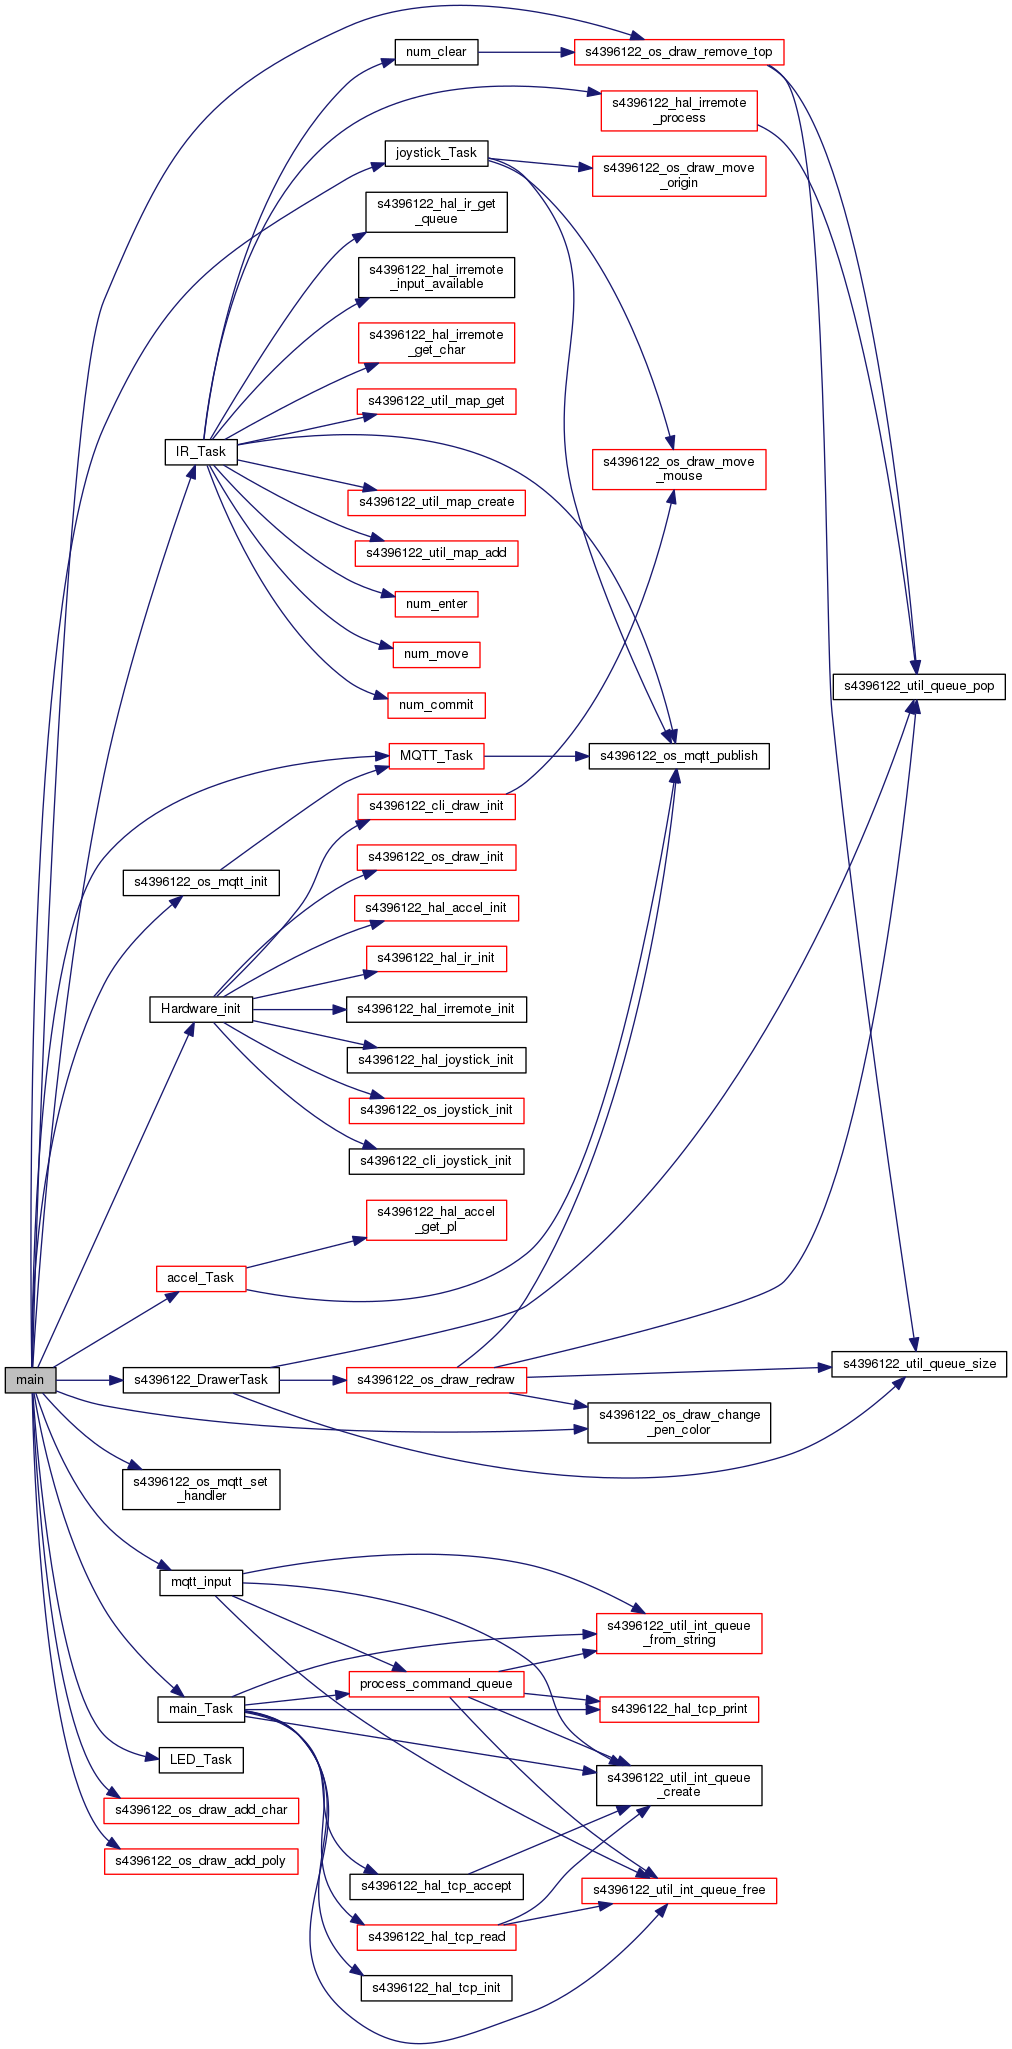
\includegraphics[height=550pt]{d0/d29/main_8c_ae66f6b31b5ad750f1fe042a706a4e3d4_cgraph}
\end{center}
\end{figure}


\index{main.\+c@{main.\+c}!mqtt\+\_\+input@{mqtt\+\_\+input}}
\index{mqtt\+\_\+input@{mqtt\+\_\+input}!main.\+c@{main.\+c}}
\subsubsection[{\texorpdfstring{mqtt\+\_\+input(char $\ast$buffer)}{mqtt_input(char *buffer)}}]{\setlength{\rightskip}{0pt plus 5cm}void mqtt\+\_\+input (
\begin{DoxyParamCaption}
\item[{char $\ast$}]{buffer}
\end{DoxyParamCaption}
)}\hypertarget{main_8c_a2a94f1a6ce73b5b0e9fa9edc1a5b1084}{}\label{main_8c_a2a94f1a6ce73b5b0e9fa9edc1a5b1084}


Called whenever there is a command sent over an mqtt connection. 


\begin{DoxyParams}{Parameters}
{\em buffer} & C\+LI input that was received \\
\hline
\end{DoxyParams}


Here is the call graph for this function\+:\nopagebreak
\begin{figure}[H]
\begin{center}
\leavevmode
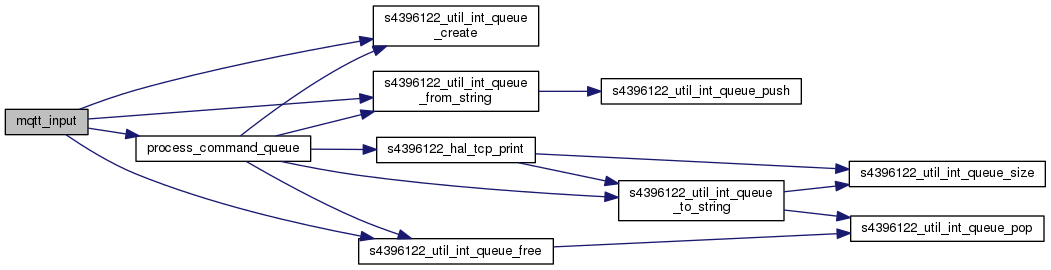
\includegraphics[width=350pt]{d0/d29/main_8c_a2a94f1a6ce73b5b0e9fa9edc1a5b1084_cgraph}
\end{center}
\end{figure}


\index{main.\+c@{main.\+c}!num\+\_\+clear@{num\+\_\+clear}}
\index{num\+\_\+clear@{num\+\_\+clear}!main.\+c@{main.\+c}}
\subsubsection[{\texorpdfstring{num\+\_\+clear(char c)}{num_clear(char c)}}]{\setlength{\rightskip}{0pt plus 5cm}void num\+\_\+clear (
\begin{DoxyParamCaption}
\item[{char}]{c}
\end{DoxyParamCaption}
)}\hypertarget{main_8c_aa6b4370f1e20551de5b33c3cb58c92f0}{}\label{main_8c_aa6b4370f1e20551de5b33c3cb58c92f0}


Handler for when the user presses the play button. 


\begin{DoxyParams}{Parameters}
{\em c} & Character that was pressed on the remote \\
\hline
\end{DoxyParams}


Here is the call graph for this function\+:\nopagebreak
\begin{figure}[H]
\begin{center}
\leavevmode
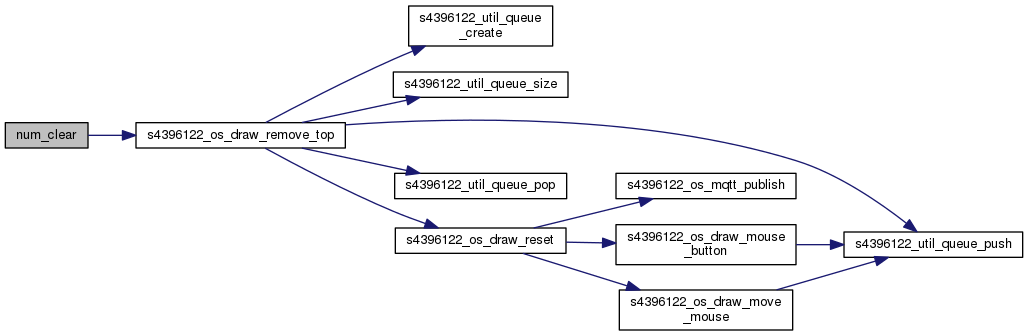
\includegraphics[width=350pt]{d0/d29/main_8c_aa6b4370f1e20551de5b33c3cb58c92f0_cgraph}
\end{center}
\end{figure}


\index{main.\+c@{main.\+c}!num\+\_\+commit@{num\+\_\+commit}}
\index{num\+\_\+commit@{num\+\_\+commit}!main.\+c@{main.\+c}}
\subsubsection[{\texorpdfstring{num\+\_\+commit(char c)}{num_commit(char c)}}]{\setlength{\rightskip}{0pt plus 5cm}void num\+\_\+commit (
\begin{DoxyParamCaption}
\item[{char}]{c}
\end{DoxyParamCaption}
)}\hypertarget{main_8c_a58bfbee9c8d80c18cd11f84d16177818}{}\label{main_8c_a58bfbee9c8d80c18cd11f84d16177818}


Handler for when the user presses the back button. 


\begin{DoxyParams}{Parameters}
{\em c} & Character that was pressed on the remote \\
\hline
\end{DoxyParams}


Here is the call graph for this function\+:\nopagebreak
\begin{figure}[H]
\begin{center}
\leavevmode
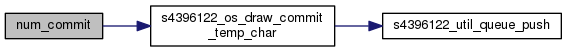
\includegraphics[width=350pt]{d0/d29/main_8c_a58bfbee9c8d80c18cd11f84d16177818_cgraph}
\end{center}
\end{figure}


\index{main.\+c@{main.\+c}!num\+\_\+enter@{num\+\_\+enter}}
\index{num\+\_\+enter@{num\+\_\+enter}!main.\+c@{main.\+c}}
\subsubsection[{\texorpdfstring{num\+\_\+enter(char c)}{num_enter(char c)}}]{\setlength{\rightskip}{0pt plus 5cm}void num\+\_\+enter (
\begin{DoxyParamCaption}
\item[{char}]{c}
\end{DoxyParamCaption}
)}\hypertarget{main_8c_aa28816a126d784c0deed58e414510a6c}{}\label{main_8c_aa28816a126d784c0deed58e414510a6c}


Handler for when a user presses a numeric button on the IR Remote. 


\begin{DoxyParams}{Parameters}
{\em c} & character representing the character pressed \\
\hline
\end{DoxyParams}
$<$ The resulting incoded char of the input 

Here is the call graph for this function\+:\nopagebreak
\begin{figure}[H]
\begin{center}
\leavevmode
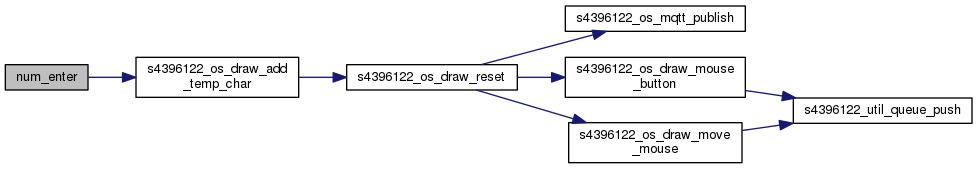
\includegraphics[width=350pt]{d0/d29/main_8c_aa28816a126d784c0deed58e414510a6c_cgraph}
\end{center}
\end{figure}


\index{main.\+c@{main.\+c}!num\+\_\+move@{num\+\_\+move}}
\index{num\+\_\+move@{num\+\_\+move}!main.\+c@{main.\+c}}
\subsubsection[{\texorpdfstring{num\+\_\+move(char c)}{num_move(char c)}}]{\setlength{\rightskip}{0pt plus 5cm}void num\+\_\+move (
\begin{DoxyParamCaption}
\item[{char}]{c}
\end{DoxyParamCaption}
)}\hypertarget{main_8c_a6de80721052311b1be7cb837c5db6887}{}\label{main_8c_a6de80721052311b1be7cb837c5db6887}


Handler for when the user presses a directional button on the IR remote. 


\begin{DoxyParams}{Parameters}
{\em c} & Character that was pressed on the remote \\
\hline
\end{DoxyParams}


Here is the call graph for this function\+:\nopagebreak
\begin{figure}[H]
\begin{center}
\leavevmode
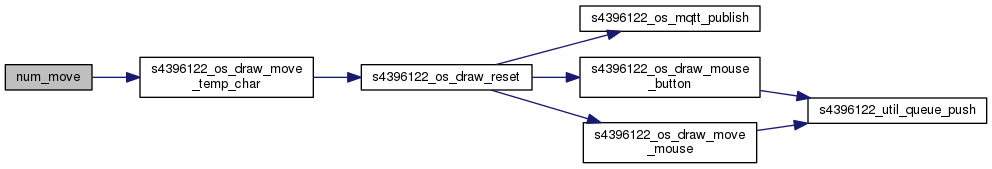
\includegraphics[width=350pt]{d0/d29/main_8c_a6de80721052311b1be7cb837c5db6887_cgraph}
\end{center}
\end{figure}


\index{main.\+c@{main.\+c}!process\+\_\+command\+\_\+queue@{process\+\_\+command\+\_\+queue}}
\index{process\+\_\+command\+\_\+queue@{process\+\_\+command\+\_\+queue}!main.\+c@{main.\+c}}
\subsubsection[{\texorpdfstring{process\+\_\+command\+\_\+queue(\+Int\+Queue $\ast$q)}{process_command_queue(IntQueue *q)}}]{\setlength{\rightskip}{0pt plus 5cm}void process\+\_\+command\+\_\+queue (
\begin{DoxyParamCaption}
\item[{{\bf Int\+Queue} $\ast$}]{q}
\end{DoxyParamCaption}
)}\hypertarget{main_8c_aded10eb51d4ca5e34c5de551c09a1e37}{}\label{main_8c_aded10eb51d4ca5e34c5de551c09a1e37}


Processes the input cli command and calls the required Free\+R\+T\+OS Command. 


\begin{DoxyParams}{Parameters}
{\em q} & \hyperlink{structIntQueue}{Int\+Queue} of the input received from the C\+LI \\
\hline
\end{DoxyParams}


Here is the call graph for this function\+:\nopagebreak
\begin{figure}[H]
\begin{center}
\leavevmode
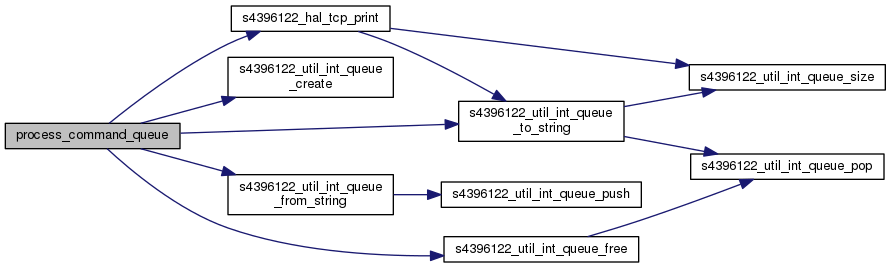
\includegraphics[width=350pt]{d0/d29/main_8c_aded10eb51d4ca5e34c5de551c09a1e37_cgraph}
\end{center}
\end{figure}


\index{main.\+c@{main.\+c}!v\+Application\+Stack\+Overflow\+Hook@{v\+Application\+Stack\+Overflow\+Hook}}
\index{v\+Application\+Stack\+Overflow\+Hook@{v\+Application\+Stack\+Overflow\+Hook}!main.\+c@{main.\+c}}
\subsubsection[{\texorpdfstring{v\+Application\+Stack\+Overflow\+Hook(x\+Task\+Handle px\+Task, signed char $\ast$pc\+Task\+Name)}{vApplicationStackOverflowHook(xTaskHandle pxTask, signed char *pcTaskName)}}]{\setlength{\rightskip}{0pt plus 5cm}void v\+Application\+Stack\+Overflow\+Hook (
\begin{DoxyParamCaption}
\item[{x\+Task\+Handle}]{px\+Task, }
\item[{signed char $\ast$}]{pc\+Task\+Name}
\end{DoxyParamCaption}
)}\hypertarget{main_8c_af82984987d75dcade423623c8f343413}{}\label{main_8c_af82984987d75dcade423623c8f343413}


Called whenever the system stack overflows. 


\begin{DoxyParams}{Parameters}
{\em px\+Task} & Task Handler for the overflowed task \\
\hline
{\em pc\+Task\+Name} & Task Name of the overflowed task \\
\hline
\end{DoxyParams}


\subsection{Variable Documentation}
\index{main.\+c@{main.\+c}!x\+Char@{x\+Char}}
\index{x\+Char@{x\+Char}!main.\+c@{main.\+c}}
\subsubsection[{\texorpdfstring{x\+Char}{xChar}}]{\setlength{\rightskip}{0pt plus 5cm}C\+L\+I\+\_\+\+Command\+\_\+\+Definition\+\_\+t x\+Char}\hypertarget{main_8c_a7aa85a9e2c0db0c3c9ed26907092c2c9}{}\label{main_8c_a7aa85a9e2c0db0c3c9ed26907092c2c9}
{\bfseries Initial value\+:}
\begin{DoxyCode}
= \{
    \textcolor{stringliteral}{"char"},
    \textcolor{stringliteral}{"char:\(\backslash\)n Draw an alphanumeric character. (x, y, c)\(\backslash\)n\(\backslash\)n"},
    prvCharCommand,
    3
\}
\end{DoxyCode}


C\+LI struct for char command. 

\index{main.\+c@{main.\+c}!x\+Clear@{x\+Clear}}
\index{x\+Clear@{x\+Clear}!main.\+c@{main.\+c}}
\subsubsection[{\texorpdfstring{x\+Clear}{xClear}}]{\setlength{\rightskip}{0pt plus 5cm}C\+L\+I\+\_\+\+Command\+\_\+\+Definition\+\_\+t x\+Clear}\hypertarget{main_8c_aa29c81f0e2db1c0d049227983352b554}{}\label{main_8c_aa29c81f0e2db1c0d049227983352b554}
{\bfseries Initial value\+:}
\begin{DoxyCode}
= \{
    \textcolor{stringliteral}{"clear"},
    \textcolor{stringliteral}{"clear:\(\backslash\)n Clear the last drawn command\(\backslash\)n\(\backslash\)n"},
    prvClearCommand,
    0
\}
\end{DoxyCode}


C\+LI struct for clear command. 

\index{main.\+c@{main.\+c}!x\+Colour@{x\+Colour}}
\index{x\+Colour@{x\+Colour}!main.\+c@{main.\+c}}
\subsubsection[{\texorpdfstring{x\+Colour}{xColour}}]{\setlength{\rightskip}{0pt plus 5cm}C\+L\+I\+\_\+\+Command\+\_\+\+Definition\+\_\+t x\+Colour}\hypertarget{main_8c_a39b07388892ed15845498794ad99235f}{}\label{main_8c_a39b07388892ed15845498794ad99235f}
{\bfseries Initial value\+:}
\begin{DoxyCode}
= \{
    \textcolor{stringliteral}{"colour"},
    \textcolor{stringliteral}{"colour:\(\backslash\)n Change the colour of the pen\(\backslash\)n\(\backslash\)n"},
    prvColourCommand,
    1
\}
\end{DoxyCode}


C\+LI struct for colour command. 

\index{main.\+c@{main.\+c}!x\+Create@{x\+Create}}
\index{x\+Create@{x\+Create}!main.\+c@{main.\+c}}
\subsubsection[{\texorpdfstring{x\+Create}{xCreate}}]{\setlength{\rightskip}{0pt plus 5cm}C\+L\+I\+\_\+\+Command\+\_\+\+Definition\+\_\+t x\+Create}\hypertarget{main_8c_a120969c3f3b0ab1a0695c0981a13811b}{}\label{main_8c_a120969c3f3b0ab1a0695c0981a13811b}
{\bfseries Initial value\+:}
\begin{DoxyCode}
= \{
    \textcolor{stringliteral}{"create"},
    \textcolor{stringliteral}{"create:\(\backslash\)n Create a mylib OS peripheral task with a given name\(\backslash\)n\(\backslash\)n"},
    prvCreateCommand,
    1
\}
\end{DoxyCode}


C\+LI struct for create command. 

\index{main.\+c@{main.\+c}!x\+Delete@{x\+Delete}}
\index{x\+Delete@{x\+Delete}!main.\+c@{main.\+c}}
\subsubsection[{\texorpdfstring{x\+Delete}{xDelete}}]{\setlength{\rightskip}{0pt plus 5cm}C\+L\+I\+\_\+\+Command\+\_\+\+Definition\+\_\+t x\+Delete}\hypertarget{main_8c_aa4021bccff839bb23b1d2dabf7885ae4}{}\label{main_8c_aa4021bccff839bb23b1d2dabf7885ae4}
{\bfseries Initial value\+:}
\begin{DoxyCode}
= \{
    \textcolor{stringliteral}{"delete"},
    \textcolor{stringliteral}{"delete:\(\backslash\)n Delete a mylib OS peripheral task with a given name\(\backslash\)n\(\backslash\)n"},
    prvDeleteCommand,
    1
\}
\end{DoxyCode}


C\+LI struct for delete command. 

\index{main.\+c@{main.\+c}!x\+Poly@{x\+Poly}}
\index{x\+Poly@{x\+Poly}!main.\+c@{main.\+c}}
\subsubsection[{\texorpdfstring{x\+Poly}{xPoly}}]{\setlength{\rightskip}{0pt plus 5cm}C\+L\+I\+\_\+\+Command\+\_\+\+Definition\+\_\+t x\+Poly}\hypertarget{main_8c_a40d863d8c7a385acffa0662848481be6}{}\label{main_8c_a40d863d8c7a385acffa0662848481be6}
{\bfseries Initial value\+:}
\begin{DoxyCode}
= \{
    \textcolor{stringliteral}{"poly"},
    \textcolor{stringliteral}{"poly:\(\backslash\)n Draw a regular polygon. (x, y, l, o)\(\backslash\)n\(\backslash\)n"},
    prvPolyCommand,
    4
\}
\end{DoxyCode}


C\+LI struct for poly command. 

\index{main.\+c@{main.\+c}!x\+Resume@{x\+Resume}}
\index{x\+Resume@{x\+Resume}!main.\+c@{main.\+c}}
\subsubsection[{\texorpdfstring{x\+Resume}{xResume}}]{\setlength{\rightskip}{0pt plus 5cm}C\+L\+I\+\_\+\+Command\+\_\+\+Definition\+\_\+t x\+Resume}\hypertarget{main_8c_a6273e15578b1a534c739ae81307ad7d3}{}\label{main_8c_a6273e15578b1a534c739ae81307ad7d3}
{\bfseries Initial value\+:}
\begin{DoxyCode}
= \{
    \textcolor{stringliteral}{"resume"},
    \textcolor{stringliteral}{"resume:\(\backslash\)n Resume a mylib OS peripheral task with a given name\(\backslash\)n\(\backslash\)n"},
    prvResumeCommand,
    1
\}
\end{DoxyCode}


C\+LI struct for resume command. 

\index{main.\+c@{main.\+c}!x\+Suspend@{x\+Suspend}}
\index{x\+Suspend@{x\+Suspend}!main.\+c@{main.\+c}}
\subsubsection[{\texorpdfstring{x\+Suspend}{xSuspend}}]{\setlength{\rightskip}{0pt plus 5cm}C\+L\+I\+\_\+\+Command\+\_\+\+Definition\+\_\+t x\+Suspend}\hypertarget{main_8c_ab08258c60fefc7dea0630027f7009f98}{}\label{main_8c_ab08258c60fefc7dea0630027f7009f98}
{\bfseries Initial value\+:}
\begin{DoxyCode}
= \{
    \textcolor{stringliteral}{"suspend"},
    \textcolor{stringliteral}{"suspend:\(\backslash\)n Suspend a mylib OS peripheral task with a given name\(\backslash\)n\(\backslash\)n"},
    prvSuspendCommand,
    1
\}
\end{DoxyCode}


C\+LI struct for suspend command. 

\index{main.\+c@{main.\+c}!x\+Text@{x\+Text}}
\index{x\+Text@{x\+Text}!main.\+c@{main.\+c}}
\subsubsection[{\texorpdfstring{x\+Text}{xText}}]{\setlength{\rightskip}{0pt plus 5cm}C\+L\+I\+\_\+\+Command\+\_\+\+Definition\+\_\+t x\+Text}\hypertarget{main_8c_a6b7973fc30ca825b5e9514cec40de2b0}{}\label{main_8c_a6b7973fc30ca825b5e9514cec40de2b0}
{\bfseries Initial value\+:}
\begin{DoxyCode}
= \{
    \textcolor{stringliteral}{"text"},
    \textcolor{stringliteral}{"text:\(\backslash\)n Draw a text string, up to 10 characters long. (x, y, str)\(\backslash\)n\(\backslash\)n"},
    prvTextCommand,
    3
\}
\end{DoxyCode}


C\+LI struct for text command. 

\index{main.\+c@{main.\+c}!x\+Time@{x\+Time}}
\index{x\+Time@{x\+Time}!main.\+c@{main.\+c}}
\subsubsection[{\texorpdfstring{x\+Time}{xTime}}]{\setlength{\rightskip}{0pt plus 5cm}C\+L\+I\+\_\+\+Command\+\_\+\+Definition\+\_\+t x\+Time}\hypertarget{main_8c_a6d87341119374942b9240d07ad06062f}{}\label{main_8c_a6d87341119374942b9240d07ad06062f}
{\bfseries Initial value\+:}
\begin{DoxyCode}
= \{
    \textcolor{stringliteral}{"time"},
    \textcolor{stringliteral}{"time:\(\backslash\)n Display how long the program has been running for.\(\backslash\)n\(\backslash\)n"},
    prvTimeCommand,
    0
\}
\end{DoxyCode}


C\+LI struct for time command. 

\index{main.\+c@{main.\+c}!x\+Top@{x\+Top}}
\index{x\+Top@{x\+Top}!main.\+c@{main.\+c}}
\subsubsection[{\texorpdfstring{x\+Top}{xTop}}]{\setlength{\rightskip}{0pt plus 5cm}C\+L\+I\+\_\+\+Command\+\_\+\+Definition\+\_\+t x\+Top}\hypertarget{main_8c_a50d7e2916f836420788253310e3a93a0}{}\label{main_8c_a50d7e2916f836420788253310e3a93a0}
{\bfseries Initial value\+:}
\begin{DoxyCode}
= \{
    \textcolor{stringliteral}{"top"},
    \textcolor{stringliteral}{"top:\(\backslash\)n List the current number of tasks running.\(\backslash\)n\(\backslash\)n"},
    prvTopCommand,
    0
\}
\end{DoxyCode}


C\+LI struct for top command. 


\hypertarget{netconfig_8h}{}\section{mylib/netconfig.h File Reference}
\label{netconfig_8h}\index{mylib/netconfig.\+h@{mylib/netconfig.\+h}}


This file contains M\+AC, IP, M\+A\+SK and Gateway address definitions.  


This graph shows which files directly or indirectly include this file\+:\nopagebreak
\begin{figure}[H]
\begin{center}
\leavevmode
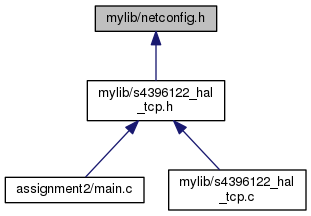
\includegraphics[width=306pt]{d3/d3d/netconfig_8h__dep__incl}
\end{center}
\end{figure}
\subsection*{Macros}
\begin{DoxyCompactItemize}
\item 
\#define {\bfseries M\+A\+C\+\_\+\+A\+D\+D\+R0}~0x02\hypertarget{netconfig_8h_ab84a2e15d360e2644ada09641513a941}{}\label{netconfig_8h_ab84a2e15d360e2644ada09641513a941}

\item 
\#define {\bfseries M\+A\+C\+\_\+\+A\+D\+D\+R1}~0x67\hypertarget{netconfig_8h_a8d14266d76690c530bee01e7e5bb4099}{}\label{netconfig_8h_a8d14266d76690c530bee01e7e5bb4099}

\item 
\#define {\bfseries M\+A\+C\+\_\+\+A\+D\+D\+R2}~0x00\hypertarget{netconfig_8h_a6c5df15bec1d305ed033ad9a85ec803d}{}\label{netconfig_8h_a6c5df15bec1d305ed033ad9a85ec803d}

\item 
\#define {\bfseries M\+A\+C\+\_\+\+A\+D\+D\+R3}~0x4A\hypertarget{netconfig_8h_a08a36ede83ae67498aecf54676be8fc8}{}\label{netconfig_8h_a08a36ede83ae67498aecf54676be8fc8}

\item 
\#define {\bfseries M\+A\+C\+\_\+\+A\+D\+D\+R4}~0x86\hypertarget{netconfig_8h_a41e5cb0b39ad74f0aafb83dbcecf9006}{}\label{netconfig_8h_a41e5cb0b39ad74f0aafb83dbcecf9006}

\item 
\#define {\bfseries M\+A\+C\+\_\+\+A\+D\+D\+R5}~0x5C\hypertarget{netconfig_8h_a3bcc92663c42ec434f527847bbc4abc1}{}\label{netconfig_8h_a3bcc92663c42ec434f527847bbc4abc1}

\item 
\#define {\bfseries I\+P\+\_\+\+A\+D\+D\+R0}~192\hypertarget{netconfig_8h_a2505da6a8f2724a8cdded72db05408db}{}\label{netconfig_8h_a2505da6a8f2724a8cdded72db05408db}

\item 
\#define {\bfseries I\+P\+\_\+\+A\+D\+D\+R1}~168\hypertarget{netconfig_8h_ac9ec1dc8780538aca0677afc96f17edb}{}\label{netconfig_8h_ac9ec1dc8780538aca0677afc96f17edb}

\item 
\#define {\bfseries I\+P\+\_\+\+A\+D\+D\+R2}~0\hypertarget{netconfig_8h_afd045706f3302adca52233444339d622}{}\label{netconfig_8h_afd045706f3302adca52233444339d622}

\item 
\#define {\bfseries I\+P\+\_\+\+A\+D\+D\+R3}~10\hypertarget{netconfig_8h_a3b2cd0c13fb411cdd9fe4e86c712f01d}{}\label{netconfig_8h_a3b2cd0c13fb411cdd9fe4e86c712f01d}

\item 
\#define {\bfseries N\+E\+T\+M\+A\+S\+K\+\_\+\+A\+D\+D\+R0}~255\hypertarget{netconfig_8h_aedc93a8d3b76cd8f395b2c7a261b1292}{}\label{netconfig_8h_aedc93a8d3b76cd8f395b2c7a261b1292}

\item 
\#define {\bfseries N\+E\+T\+M\+A\+S\+K\+\_\+\+A\+D\+D\+R1}~255\hypertarget{netconfig_8h_ae87b5d58bcdbe0f96203d250a34ee998}{}\label{netconfig_8h_ae87b5d58bcdbe0f96203d250a34ee998}

\item 
\#define {\bfseries N\+E\+T\+M\+A\+S\+K\+\_\+\+A\+D\+D\+R2}~255\hypertarget{netconfig_8h_aa663e0e0e7b04e6217a3745cbf70b35e}{}\label{netconfig_8h_aa663e0e0e7b04e6217a3745cbf70b35e}

\item 
\#define {\bfseries N\+E\+T\+M\+A\+S\+K\+\_\+\+A\+D\+D\+R3}~0\hypertarget{netconfig_8h_a85e7e72009ec7bdf398696e2646ddab2}{}\label{netconfig_8h_a85e7e72009ec7bdf398696e2646ddab2}

\item 
\#define {\bfseries G\+W\+\_\+\+A\+D\+D\+R0}~192\hypertarget{netconfig_8h_a625cbbf83ab3388b1fda6e41a8a9fbe3}{}\label{netconfig_8h_a625cbbf83ab3388b1fda6e41a8a9fbe3}

\item 
\#define {\bfseries G\+W\+\_\+\+A\+D\+D\+R1}~168\hypertarget{netconfig_8h_a7233f827b2df99f7413a8234b5573d18}{}\label{netconfig_8h_a7233f827b2df99f7413a8234b5573d18}

\item 
\#define {\bfseries G\+W\+\_\+\+A\+D\+D\+R2}~0\hypertarget{netconfig_8h_a4fc95e7b1cb3fb0e1e1eacdd2a9be7fb}{}\label{netconfig_8h_a4fc95e7b1cb3fb0e1e1eacdd2a9be7fb}

\item 
\#define {\bfseries G\+W\+\_\+\+A\+D\+D\+R3}~1\hypertarget{netconfig_8h_ab53708044283f7d5324e737295449733}{}\label{netconfig_8h_ab53708044283f7d5324e737295449733}

\end{DoxyCompactItemize}


\subsection{Detailed Description}
This file contains M\+AC, IP, M\+A\+SK and Gateway address definitions. 

\begin{DoxyAuthor}{Author}
M\+DS 
\end{DoxyAuthor}
\begin{DoxyDate}{Date}
22-\/\+April-\/2014 
\end{DoxyDate}

\hypertarget{s4396122__cli__draw_8c}{}\section{mylib/s4396122\+\_\+cli\+\_\+draw.c File Reference}
\label{s4396122__cli__draw_8c}\index{mylib/s4396122\+\_\+cli\+\_\+draw.\+c@{mylib/s4396122\+\_\+cli\+\_\+draw.\+c}}


Provides drawing commands for C\+LI.  


{\ttfamily \#include \char`\"{}s4396122\+\_\+cli\+\_\+draw.\+h\char`\"{}}\\*
Include dependency graph for s4396122\+\_\+cli\+\_\+draw.\+c\+:\nopagebreak
\begin{figure}[H]
\begin{center}
\leavevmode
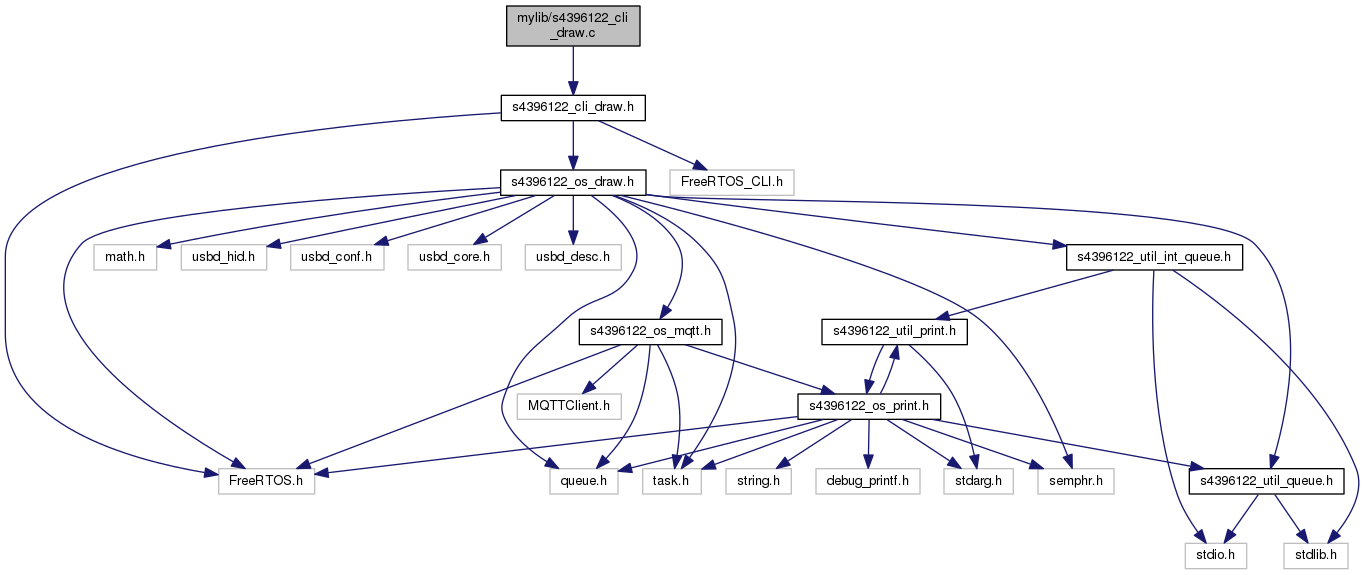
\includegraphics[width=350pt]{da/d00/s4396122__cli__draw_8c__incl}
\end{center}
\end{figure}
\subsection*{Functions}
\begin{DoxyCompactItemize}
\item 
void \hyperlink{s4396122__cli__draw_8c_ac046113876d482709dd25092711322ce}{s4396122\+\_\+cli\+\_\+draw\+\_\+init} ()\hypertarget{s4396122__cli__draw_8c_ac046113876d482709dd25092711322ce}{}\label{s4396122__cli__draw_8c_ac046113876d482709dd25092711322ce}

\begin{DoxyCompactList}\small\item\em Init function for the draw commands. Adds all the commands to Free\+R\+T\+OS. \end{DoxyCompactList}\end{DoxyCompactItemize}
\subsection*{Variables}
\begin{DoxyCompactItemize}
\item 
C\+L\+I\+\_\+\+Command\+\_\+\+Definition\+\_\+t \hyperlink{s4396122__cli__draw_8c_a703fe14e78e9274c62e285e7e8c1f004}{x\+Move}
\begin{DoxyCompactList}\small\item\em C\+LI struct for the move command. \end{DoxyCompactList}\item 
C\+L\+I\+\_\+\+Command\+\_\+\+Definition\+\_\+t \hyperlink{s4396122__cli__draw_8c_a0bbf1f58a384038b644f04a029210ae7}{x\+Pen\+Down}
\begin{DoxyCompactList}\small\item\em C\+LI struct for the pendown command. \end{DoxyCompactList}\item 
C\+L\+I\+\_\+\+Command\+\_\+\+Definition\+\_\+t \hyperlink{s4396122__cli__draw_8c_a12f286597dc033040f7b69f0e344824c}{x\+Pen\+Up}
\begin{DoxyCompactList}\small\item\em C\+LI struct for the penup command. \end{DoxyCompactList}\item 
C\+L\+I\+\_\+\+Command\+\_\+\+Definition\+\_\+t \hyperlink{s4396122__cli__draw_8c_a7f00f5ae22651ea80ed6c0e1175197d5}{x\+Box}
\begin{DoxyCompactList}\small\item\em C\+LI struct for the box command. \end{DoxyCompactList}\item 
C\+L\+I\+\_\+\+Command\+\_\+\+Definition\+\_\+t \hyperlink{s4396122__cli__draw_8c_a092af686c934dca8f9c868855a963b74}{x\+Line}
\begin{DoxyCompactList}\small\item\em C\+LI struct for the line command. \end{DoxyCompactList}\item 
C\+L\+I\+\_\+\+Command\+\_\+\+Definition\+\_\+t \hyperlink{s4396122__cli__draw_8c_a55ac17ca54e87f6e4f9c9a45c02befaa}{x\+Reset}
\begin{DoxyCompactList}\small\item\em C\+LI struct for the reset command. \end{DoxyCompactList}\item 
C\+L\+I\+\_\+\+Command\+\_\+\+Definition\+\_\+t \hyperlink{s4396122__cli__draw_8c_afef7211ac1797958876a7aefadcd9180}{x\+Pen}
\begin{DoxyCompactList}\small\item\em C\+LI struct for the pen command. \end{DoxyCompactList}\item 
C\+L\+I\+\_\+\+Command\+\_\+\+Definition\+\_\+t \hyperlink{s4396122__cli__draw_8c_ac6d6240194b16683e24d20a358b10eda}{x\+Rotate}
\begin{DoxyCompactList}\small\item\em C\+LI struct for the rotate command. \end{DoxyCompactList}\end{DoxyCompactItemize}


\subsection{Detailed Description}
Provides drawing commands for C\+LI. 

\begin{DoxyAuthor}{Author}
Daniel Fitzmaurice -\/ 43961229 
\end{DoxyAuthor}
\begin{DoxyVersion}{Version}
1 
\end{DoxyVersion}
\begin{DoxyDate}{Date}
2017-\/05-\/31 
\end{DoxyDate}


\subsection{Variable Documentation}
\index{s4396122\+\_\+cli\+\_\+draw.\+c@{s4396122\+\_\+cli\+\_\+draw.\+c}!x\+Box@{x\+Box}}
\index{x\+Box@{x\+Box}!s4396122\+\_\+cli\+\_\+draw.\+c@{s4396122\+\_\+cli\+\_\+draw.\+c}}
\subsubsection[{\texorpdfstring{x\+Box}{xBox}}]{\setlength{\rightskip}{0pt plus 5cm}C\+L\+I\+\_\+\+Command\+\_\+\+Definition\+\_\+t x\+Box}\hypertarget{s4396122__cli__draw_8c_a7f00f5ae22651ea80ed6c0e1175197d5}{}\label{s4396122__cli__draw_8c_a7f00f5ae22651ea80ed6c0e1175197d5}
{\bfseries Initial value\+:}
\begin{DoxyCode}
= \{
    \textcolor{stringliteral}{"box"},
    \textcolor{stringliteral}{"box:\(\backslash\)n Draw a box on the screen in the center.\(\backslash\)n\(\backslash\)n"},
    prvBoxCommand,
    0
\}
\end{DoxyCode}


C\+LI struct for the box command. 

\index{s4396122\+\_\+cli\+\_\+draw.\+c@{s4396122\+\_\+cli\+\_\+draw.\+c}!x\+Line@{x\+Line}}
\index{x\+Line@{x\+Line}!s4396122\+\_\+cli\+\_\+draw.\+c@{s4396122\+\_\+cli\+\_\+draw.\+c}}
\subsubsection[{\texorpdfstring{x\+Line}{xLine}}]{\setlength{\rightskip}{0pt plus 5cm}C\+L\+I\+\_\+\+Command\+\_\+\+Definition\+\_\+t x\+Line}\hypertarget{s4396122__cli__draw_8c_a092af686c934dca8f9c868855a963b74}{}\label{s4396122__cli__draw_8c_a092af686c934dca8f9c868855a963b74}
{\bfseries Initial value\+:}
\begin{DoxyCode}
= \{
    \textcolor{stringliteral}{"line"},
    \textcolor{stringliteral}{"line:\(\backslash\)n Draw a line from x1 y1 to x2 y2. \{(x1 y1) (x2 y2)\}\(\backslash\)n\(\backslash\)n"},
    prvLineCommand,
    4
\}
\end{DoxyCode}


C\+LI struct for the line command. 

\index{s4396122\+\_\+cli\+\_\+draw.\+c@{s4396122\+\_\+cli\+\_\+draw.\+c}!x\+Move@{x\+Move}}
\index{x\+Move@{x\+Move}!s4396122\+\_\+cli\+\_\+draw.\+c@{s4396122\+\_\+cli\+\_\+draw.\+c}}
\subsubsection[{\texorpdfstring{x\+Move}{xMove}}]{\setlength{\rightskip}{0pt plus 5cm}C\+L\+I\+\_\+\+Command\+\_\+\+Definition\+\_\+t x\+Move}\hypertarget{s4396122__cli__draw_8c_a703fe14e78e9274c62e285e7e8c1f004}{}\label{s4396122__cli__draw_8c_a703fe14e78e9274c62e285e7e8c1f004}
{\bfseries Initial value\+:}
\begin{DoxyCode}
= \{
    \textcolor{stringliteral}{"move"},
    \textcolor{stringliteral}{"move:\(\backslash\)n Move the cursor by the x and y position.\(\backslash\)n\(\backslash\)n"},
    prvMoveCommand,
    2
\}
\end{DoxyCode}


C\+LI struct for the move command. 

\index{s4396122\+\_\+cli\+\_\+draw.\+c@{s4396122\+\_\+cli\+\_\+draw.\+c}!x\+Pen@{x\+Pen}}
\index{x\+Pen@{x\+Pen}!s4396122\+\_\+cli\+\_\+draw.\+c@{s4396122\+\_\+cli\+\_\+draw.\+c}}
\subsubsection[{\texorpdfstring{x\+Pen}{xPen}}]{\setlength{\rightskip}{0pt plus 5cm}C\+L\+I\+\_\+\+Command\+\_\+\+Definition\+\_\+t x\+Pen}\hypertarget{s4396122__cli__draw_8c_afef7211ac1797958876a7aefadcd9180}{}\label{s4396122__cli__draw_8c_afef7211ac1797958876a7aefadcd9180}
{\bfseries Initial value\+:}
\begin{DoxyCode}
= \{
    \textcolor{stringliteral}{"pen"},
    \textcolor{stringliteral}{"pen:\(\backslash\)n Sets the type of pen for drawing with.\(\backslash\)n\(\backslash\)n"},
    prvPenCommand,
    1
\}
\end{DoxyCode}


C\+LI struct for the pen command. 

\index{s4396122\+\_\+cli\+\_\+draw.\+c@{s4396122\+\_\+cli\+\_\+draw.\+c}!x\+Pen\+Down@{x\+Pen\+Down}}
\index{x\+Pen\+Down@{x\+Pen\+Down}!s4396122\+\_\+cli\+\_\+draw.\+c@{s4396122\+\_\+cli\+\_\+draw.\+c}}
\subsubsection[{\texorpdfstring{x\+Pen\+Down}{xPenDown}}]{\setlength{\rightskip}{0pt plus 5cm}C\+L\+I\+\_\+\+Command\+\_\+\+Definition\+\_\+t x\+Pen\+Down}\hypertarget{s4396122__cli__draw_8c_a0bbf1f58a384038b644f04a029210ae7}{}\label{s4396122__cli__draw_8c_a0bbf1f58a384038b644f04a029210ae7}
{\bfseries Initial value\+:}
\begin{DoxyCode}
= \{
    \textcolor{stringliteral}{"pendown"},
    \textcolor{stringliteral}{"pendown:\(\backslash\)n Puts the pen down on the screen.\(\backslash\)n\(\backslash\)n"},
    prvPenDownCommand,
    0
\}
\end{DoxyCode}


C\+LI struct for the pendown command. 

\index{s4396122\+\_\+cli\+\_\+draw.\+c@{s4396122\+\_\+cli\+\_\+draw.\+c}!x\+Pen\+Up@{x\+Pen\+Up}}
\index{x\+Pen\+Up@{x\+Pen\+Up}!s4396122\+\_\+cli\+\_\+draw.\+c@{s4396122\+\_\+cli\+\_\+draw.\+c}}
\subsubsection[{\texorpdfstring{x\+Pen\+Up}{xPenUp}}]{\setlength{\rightskip}{0pt plus 5cm}C\+L\+I\+\_\+\+Command\+\_\+\+Definition\+\_\+t x\+Pen\+Up}\hypertarget{s4396122__cli__draw_8c_a12f286597dc033040f7b69f0e344824c}{}\label{s4396122__cli__draw_8c_a12f286597dc033040f7b69f0e344824c}
{\bfseries Initial value\+:}
\begin{DoxyCode}
= \{
    \textcolor{stringliteral}{"penup"},
    \textcolor{stringliteral}{"penup:\(\backslash\)n Releases the pen from the screen.\(\backslash\)n\(\backslash\)n"},
    prvPenUpCommand,
    0
\}
\end{DoxyCode}


C\+LI struct for the penup command. 

\index{s4396122\+\_\+cli\+\_\+draw.\+c@{s4396122\+\_\+cli\+\_\+draw.\+c}!x\+Reset@{x\+Reset}}
\index{x\+Reset@{x\+Reset}!s4396122\+\_\+cli\+\_\+draw.\+c@{s4396122\+\_\+cli\+\_\+draw.\+c}}
\subsubsection[{\texorpdfstring{x\+Reset}{xReset}}]{\setlength{\rightskip}{0pt plus 5cm}C\+L\+I\+\_\+\+Command\+\_\+\+Definition\+\_\+t x\+Reset}\hypertarget{s4396122__cli__draw_8c_a55ac17ca54e87f6e4f9c9a45c02befaa}{}\label{s4396122__cli__draw_8c_a55ac17ca54e87f6e4f9c9a45c02befaa}
{\bfseries Initial value\+:}
\begin{DoxyCode}
= \{
    \textcolor{stringliteral}{"reset"},
    \textcolor{stringliteral}{"reset:\(\backslash\)n Clears the canvas for a fresh drawing\(\backslash\)n\(\backslash\)n"},
    prvResetCommand,
    0
\}
\end{DoxyCode}


C\+LI struct for the reset command. 

\index{s4396122\+\_\+cli\+\_\+draw.\+c@{s4396122\+\_\+cli\+\_\+draw.\+c}!x\+Rotate@{x\+Rotate}}
\index{x\+Rotate@{x\+Rotate}!s4396122\+\_\+cli\+\_\+draw.\+c@{s4396122\+\_\+cli\+\_\+draw.\+c}}
\subsubsection[{\texorpdfstring{x\+Rotate}{xRotate}}]{\setlength{\rightskip}{0pt plus 5cm}C\+L\+I\+\_\+\+Command\+\_\+\+Definition\+\_\+t x\+Rotate}\hypertarget{s4396122__cli__draw_8c_ac6d6240194b16683e24d20a358b10eda}{}\label{s4396122__cli__draw_8c_ac6d6240194b16683e24d20a358b10eda}
{\bfseries Initial value\+:}
\begin{DoxyCode}
= \{
    \textcolor{stringliteral}{"rotate"},
    \textcolor{stringliteral}{"rotate:\(\backslash\)n Changes the drawing orientation\(\backslash\)n\(\backslash\)n"},
    prvRotateCommand,
    1
\}
\end{DoxyCode}


C\+LI struct for the rotate command. 


\hypertarget{s4396122__cli__draw_8h}{}\section{mylib/s4396122\+\_\+cli\+\_\+draw.h File Reference}
\label{s4396122__cli__draw_8h}\index{mylib/s4396122\+\_\+cli\+\_\+draw.\+h@{mylib/s4396122\+\_\+cli\+\_\+draw.\+h}}


Provides drawing commands for C\+LI.  


{\ttfamily \#include \char`\"{}s4396122\+\_\+os\+\_\+draw.\+h\char`\"{}}\\*
{\ttfamily \#include \char`\"{}Free\+R\+T\+O\+S.\+h\char`\"{}}\\*
{\ttfamily \#include \char`\"{}Free\+R\+T\+O\+S\+\_\+\+C\+L\+I.\+h\char`\"{}}\\*
Include dependency graph for s4396122\+\_\+cli\+\_\+draw.\+h\+:\nopagebreak
\begin{figure}[H]
\begin{center}
\leavevmode
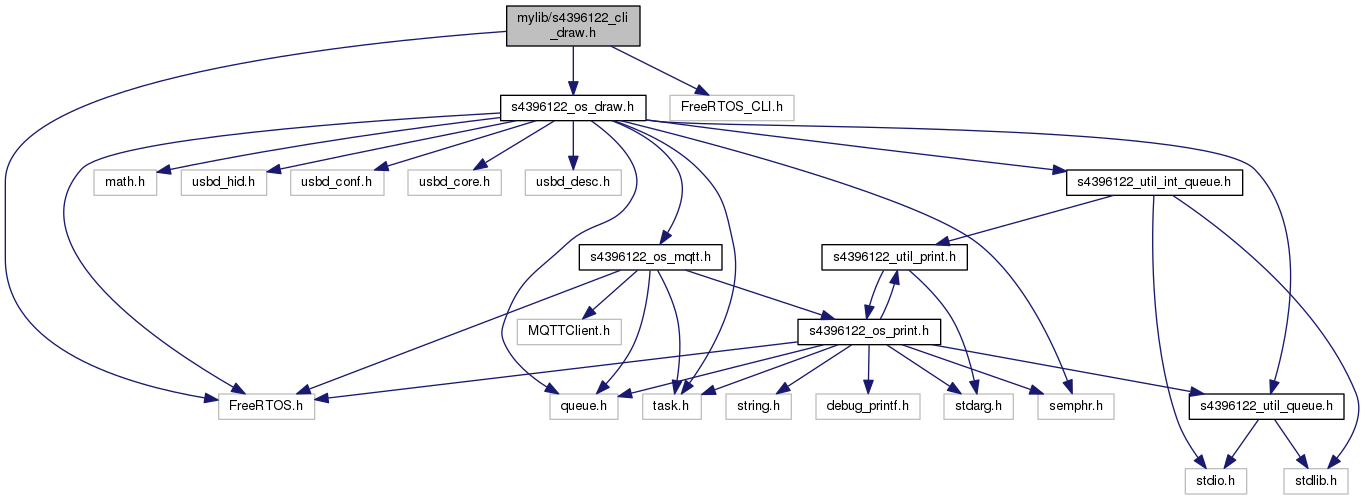
\includegraphics[width=350pt]{da/d5a/s4396122__cli__draw_8h__incl}
\end{center}
\end{figure}
This graph shows which files directly or indirectly include this file\+:\nopagebreak
\begin{figure}[H]
\begin{center}
\leavevmode
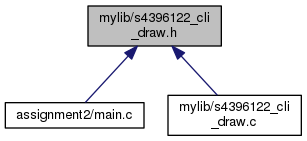
\includegraphics[width=302pt]{dd/d75/s4396122__cli__draw_8h__dep__incl}
\end{center}
\end{figure}
\subsection*{Functions}
\begin{DoxyCompactItemize}
\item 
void \hyperlink{s4396122__cli__draw_8h_ac046113876d482709dd25092711322ce}{s4396122\+\_\+cli\+\_\+draw\+\_\+init} ()\hypertarget{s4396122__cli__draw_8h_ac046113876d482709dd25092711322ce}{}\label{s4396122__cli__draw_8h_ac046113876d482709dd25092711322ce}

\begin{DoxyCompactList}\small\item\em Init function for the draw commands. Adds all the commands to Free\+R\+T\+OS. \end{DoxyCompactList}\end{DoxyCompactItemize}


\subsection{Detailed Description}
Provides drawing commands for C\+LI. 

\begin{DoxyAuthor}{Author}
Daniel Fitzmaurice -\/ 43961229 
\end{DoxyAuthor}
\begin{DoxyVersion}{Version}
1 
\end{DoxyVersion}
\begin{DoxyDate}{Date}
2017-\/05-\/31 
\end{DoxyDate}

\hypertarget{s4396122__cli__joystick_8c}{}\section{mylib/s4396122\+\_\+cli\+\_\+joystick.c File Reference}
\label{s4396122__cli__joystick_8c}\index{mylib/s4396122\+\_\+cli\+\_\+joystick.\+c@{mylib/s4396122\+\_\+cli\+\_\+joystick.\+c}}


Provides joystick commands for C\+LI.  


{\ttfamily \#include \char`\"{}s4396122\+\_\+cli\+\_\+joystick.\+h\char`\"{}}\\*
Include dependency graph for s4396122\+\_\+cli\+\_\+joystick.\+c\+:\nopagebreak
\begin{figure}[H]
\begin{center}
\leavevmode
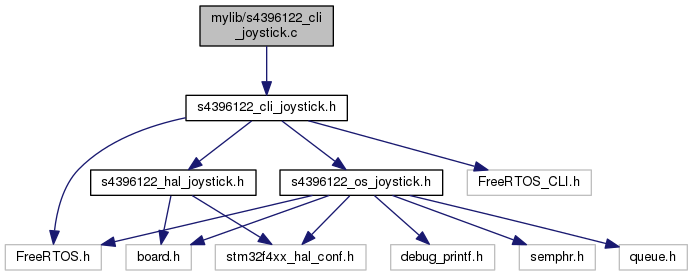
\includegraphics[width=350pt]{d7/d92/s4396122__cli__joystick_8c__incl}
\end{center}
\end{figure}
\subsection*{Functions}
\begin{DoxyCompactItemize}
\item 
void \hyperlink{s4396122__cli__joystick_8c_a3c5d12dc9250d5381efd75052843df38}{s4396122\+\_\+cli\+\_\+joystick\+\_\+init} ()\hypertarget{s4396122__cli__joystick_8c_a3c5d12dc9250d5381efd75052843df38}{}\label{s4396122__cli__joystick_8c_a3c5d12dc9250d5381efd75052843df38}

\begin{DoxyCompactList}\small\item\em Init function for the joystick commands. Adds all the commands to Free\+R\+T\+OS. \end{DoxyCompactList}\end{DoxyCompactItemize}
\subsection*{Variables}
\begin{DoxyCompactItemize}
\item 
C\+L\+I\+\_\+\+Command\+\_\+\+Definition\+\_\+t \hyperlink{s4396122__cli__joystick_8c_a969f540204313581bfbc2b9b812ab743}{x\+Joystick}
\begin{DoxyCompactList}\small\item\em C\+LI struct for the joystick command. \end{DoxyCompactList}\end{DoxyCompactItemize}


\subsection{Detailed Description}
Provides joystick commands for C\+LI. 

\begin{DoxyAuthor}{Author}
Daniel Fitzmaurice -\/ 43961229 
\end{DoxyAuthor}
\begin{DoxyVersion}{Version}
1 
\end{DoxyVersion}
\begin{DoxyDate}{Date}
2017-\/05-\/31 
\end{DoxyDate}


\subsection{Variable Documentation}
\index{s4396122\+\_\+cli\+\_\+joystick.\+c@{s4396122\+\_\+cli\+\_\+joystick.\+c}!x\+Joystick@{x\+Joystick}}
\index{x\+Joystick@{x\+Joystick}!s4396122\+\_\+cli\+\_\+joystick.\+c@{s4396122\+\_\+cli\+\_\+joystick.\+c}}
\subsubsection[{\texorpdfstring{x\+Joystick}{xJoystick}}]{\setlength{\rightskip}{0pt plus 5cm}C\+L\+I\+\_\+\+Command\+\_\+\+Definition\+\_\+t x\+Joystick}\hypertarget{s4396122__cli__joystick_8c_a969f540204313581bfbc2b9b812ab743}{}\label{s4396122__cli__joystick_8c_a969f540204313581bfbc2b9b812ab743}
{\bfseries Initial value\+:}
\begin{DoxyCode}
= \{
    \textcolor{stringliteral}{"joystick"},
    \textcolor{stringliteral}{"joystick:\(\backslash\)n Return the joystick vector.\(\backslash\)n\(\backslash\)n"},
    prvJoystickCommand,
    0
\}
\end{DoxyCode}


C\+LI struct for the joystick command. 


\hypertarget{s4396122__cli__joystick_8h}{}\section{mylib/s4396122\+\_\+cli\+\_\+joystick.h File Reference}
\label{s4396122__cli__joystick_8h}\index{mylib/s4396122\+\_\+cli\+\_\+joystick.\+h@{mylib/s4396122\+\_\+cli\+\_\+joystick.\+h}}


Provides joystick commands for C\+LI.  


{\ttfamily \#include \char`\"{}Free\+R\+T\+O\+S.\+h\char`\"{}}\\*
{\ttfamily \#include \char`\"{}Free\+R\+T\+O\+S\+\_\+\+C\+L\+I.\+h\char`\"{}}\\*
{\ttfamily \#include \char`\"{}s4396122\+\_\+os\+\_\+joystick.\+h\char`\"{}}\\*
{\ttfamily \#include \char`\"{}s4396122\+\_\+hal\+\_\+joystick.\+h\char`\"{}}\\*
Include dependency graph for s4396122\+\_\+cli\+\_\+joystick.\+h\+:\nopagebreak
\begin{figure}[H]
\begin{center}
\leavevmode
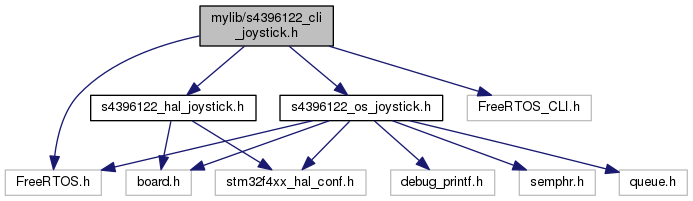
\includegraphics[width=350pt]{df/d26/s4396122__cli__joystick_8h__incl}
\end{center}
\end{figure}
This graph shows which files directly or indirectly include this file\+:\nopagebreak
\begin{figure}[H]
\begin{center}
\leavevmode
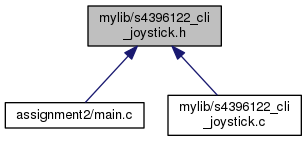
\includegraphics[width=302pt]{d6/d5c/s4396122__cli__joystick_8h__dep__incl}
\end{center}
\end{figure}
\subsection*{Functions}
\begin{DoxyCompactItemize}
\item 
void \hyperlink{s4396122__cli__joystick_8h_a3c5d12dc9250d5381efd75052843df38}{s4396122\+\_\+cli\+\_\+joystick\+\_\+init} ()\hypertarget{s4396122__cli__joystick_8h_a3c5d12dc9250d5381efd75052843df38}{}\label{s4396122__cli__joystick_8h_a3c5d12dc9250d5381efd75052843df38}

\begin{DoxyCompactList}\small\item\em Init function for the joystick commands. Adds all the commands to Free\+R\+T\+OS. \end{DoxyCompactList}\end{DoxyCompactItemize}


\subsection{Detailed Description}
Provides joystick commands for C\+LI. 

\begin{DoxyAuthor}{Author}
Daniel Fitzmaurice -\/ 43961229 
\end{DoxyAuthor}
\begin{DoxyVersion}{Version}
1 
\end{DoxyVersion}
\begin{DoxyDate}{Date}
2017-\/05-\/31 
\end{DoxyDate}

\hypertarget{s4396122__hal__accel_8c}{}\section{mylib/s4396122\+\_\+hal\+\_\+accel.c File Reference}
\label{s4396122__hal__accel_8c}\index{mylib/s4396122\+\_\+hal\+\_\+accel.\+c@{mylib/s4396122\+\_\+hal\+\_\+accel.\+c}}


Library for accessing and controlling the accelerometer.  


{\ttfamily \#include \char`\"{}s4396122\+\_\+hal\+\_\+accel.\+h\char`\"{}}\\*
Include dependency graph for s4396122\+\_\+hal\+\_\+accel.\+c\+:\nopagebreak
\begin{figure}[H]
\begin{center}
\leavevmode
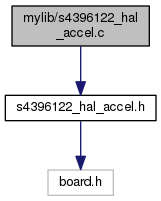
\includegraphics[width=193pt]{d7/d77/s4396122__hal__accel_8c__incl}
\end{center}
\end{figure}
\subsection*{Functions}
\begin{DoxyCompactItemize}
\item 
int \hyperlink{s4396122__hal__accel_8c_a4727344fadd3035818b45c6b949eb5b5}{read\+Register} (int addr)
\begin{DoxyCompactList}\small\item\em Reads a particular register from the I2C device. \end{DoxyCompactList}\item 
void \hyperlink{s4396122__hal__accel_8c_a32e56f6498515d5b74755c79948f5062}{s4396122\+\_\+hal\+\_\+accel\+\_\+init} ()\hypertarget{s4396122__hal__accel_8c_a32e56f6498515d5b74755c79948f5062}{}\label{s4396122__hal__accel_8c_a32e56f6498515d5b74755c79948f5062}

\begin{DoxyCompactList}\small\item\em Inits the accelerometer and any required hardware. \end{DoxyCompactList}\item 
struct \hyperlink{structPortLand}{Port\+Land} \hyperlink{s4396122__hal__accel_8c_a7c6ddaf7d43db64f178bcf2f416d4ad6}{s4396122\+\_\+hal\+\_\+accel\+\_\+get\+\_\+pl} ()
\begin{DoxyCompactList}\small\item\em Returns the result if the system is portrait or landscape. \end{DoxyCompactList}\end{DoxyCompactItemize}
\subsection*{Variables}
\begin{DoxyCompactItemize}
\item 
I2\+C\+\_\+\+Handle\+Type\+Def \hyperlink{s4396122__hal__accel_8c_a55a03c76876b7a442bac67ab50bcbc11}{I2\+C\+Handle}\hypertarget{s4396122__hal__accel_8c_a55a03c76876b7a442bac67ab50bcbc11}{}\label{s4396122__hal__accel_8c_a55a03c76876b7a442bac67ab50bcbc11}

\begin{DoxyCompactList}\small\item\em Handler for the I2C interface. \end{DoxyCompactList}\end{DoxyCompactItemize}


\subsection{Detailed Description}
Library for accessing and controlling the accelerometer. 

\begin{DoxyAuthor}{Author}
Daniel Fitzmaurice -\/ 43961229 
\end{DoxyAuthor}
\begin{DoxyVersion}{Version}
1 
\end{DoxyVersion}
\begin{DoxyDate}{Date}
2017-\/05-\/31 
\end{DoxyDate}


\subsection{Function Documentation}
\index{s4396122\+\_\+hal\+\_\+accel.\+c@{s4396122\+\_\+hal\+\_\+accel.\+c}!read\+Register@{read\+Register}}
\index{read\+Register@{read\+Register}!s4396122\+\_\+hal\+\_\+accel.\+c@{s4396122\+\_\+hal\+\_\+accel.\+c}}
\subsubsection[{\texorpdfstring{read\+Register(int addr)}{readRegister(int addr)}}]{\setlength{\rightskip}{0pt plus 5cm}int read\+Register (
\begin{DoxyParamCaption}
\item[{int}]{addr}
\end{DoxyParamCaption}
)}\hypertarget{s4396122__hal__accel_8c_a4727344fadd3035818b45c6b949eb5b5}{}\label{s4396122__hal__accel_8c_a4727344fadd3035818b45c6b949eb5b5}


Reads a particular register from the I2C device. 


\begin{DoxyParams}{Parameters}
{\em addr} & Register address to read from\\
\hline
\end{DoxyParams}
\begin{DoxyReturn}{Returns}
value read from the register 
\end{DoxyReturn}
\index{s4396122\+\_\+hal\+\_\+accel.\+c@{s4396122\+\_\+hal\+\_\+accel.\+c}!s4396122\+\_\+hal\+\_\+accel\+\_\+get\+\_\+pl@{s4396122\+\_\+hal\+\_\+accel\+\_\+get\+\_\+pl}}
\index{s4396122\+\_\+hal\+\_\+accel\+\_\+get\+\_\+pl@{s4396122\+\_\+hal\+\_\+accel\+\_\+get\+\_\+pl}!s4396122\+\_\+hal\+\_\+accel.\+c@{s4396122\+\_\+hal\+\_\+accel.\+c}}
\subsubsection[{\texorpdfstring{s4396122\+\_\+hal\+\_\+accel\+\_\+get\+\_\+pl()}{s4396122_hal_accel_get_pl()}}]{\setlength{\rightskip}{0pt plus 5cm}struct {\bf Port\+Land} s4396122\+\_\+hal\+\_\+accel\+\_\+get\+\_\+pl (
\begin{DoxyParamCaption}
{}
\end{DoxyParamCaption}
)}\hypertarget{s4396122__hal__accel_8c_a7c6ddaf7d43db64f178bcf2f416d4ad6}{}\label{s4396122__hal__accel_8c_a7c6ddaf7d43db64f178bcf2f416d4ad6}


Returns the result if the system is portrait or landscape. 

\begin{DoxyReturn}{Returns}
Struct containing the result if the system is landscape or portrait 
\end{DoxyReturn}


Here is the call graph for this function\+:\nopagebreak
\begin{figure}[H]
\begin{center}
\leavevmode
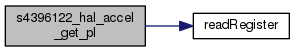
\includegraphics[width=293pt]{df/d63/s4396122__hal__accel_8c_a7c6ddaf7d43db64f178bcf2f416d4ad6_cgraph}
\end{center}
\end{figure}



\hypertarget{s4396122__hal__accel_8h}{}\section{mylib/s4396122\+\_\+hal\+\_\+accel.h File Reference}
\label{s4396122__hal__accel_8h}\index{mylib/s4396122\+\_\+hal\+\_\+accel.\+h@{mylib/s4396122\+\_\+hal\+\_\+accel.\+h}}


Library for accessing and controlling the accelerometer.  


{\ttfamily \#include \char`\"{}board.\+h\char`\"{}}\\*
Include dependency graph for s4396122\+\_\+hal\+\_\+accel.\+h\+:\nopagebreak
\begin{figure}[H]
\begin{center}
\leavevmode
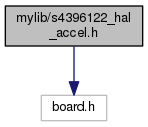
\includegraphics[width=183pt]{df/dfd/s4396122__hal__accel_8h__incl}
\end{center}
\end{figure}
This graph shows which files directly or indirectly include this file\+:\nopagebreak
\begin{figure}[H]
\begin{center}
\leavevmode
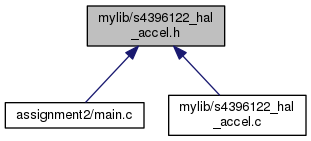
\includegraphics[width=306pt]{d9/da8/s4396122__hal__accel_8h__dep__incl}
\end{center}
\end{figure}
\subsection*{Data Structures}
\begin{DoxyCompactItemize}
\item 
struct \hyperlink{structPortLand}{Port\+Land}
\begin{DoxyCompactList}\small\item\em structure for containing the result of the pl register of the accelerometer \end{DoxyCompactList}\end{DoxyCompactItemize}
\subsection*{Macros}
\begin{DoxyCompactItemize}
\item 
\#define \hyperlink{s4396122__hal__accel_8h_a93e08213230ba022b1e70ea9e0b162a3}{M\+M\+A8452\+Q\+\_\+\+A\+D\+D\+R\+E\+SS}~(0x1\+D $<$$<$ 1)\hypertarget{s4396122__hal__accel_8h_a93e08213230ba022b1e70ea9e0b162a3}{}\label{s4396122__hal__accel_8h_a93e08213230ba022b1e70ea9e0b162a3}

\begin{DoxyCompactList}\small\item\em Address of the accelerometer. \end{DoxyCompactList}\end{DoxyCompactItemize}
\subsection*{Functions}
\begin{DoxyCompactItemize}
\item 
void \hyperlink{s4396122__hal__accel_8h_a32e56f6498515d5b74755c79948f5062}{s4396122\+\_\+hal\+\_\+accel\+\_\+init} ()\hypertarget{s4396122__hal__accel_8h_a32e56f6498515d5b74755c79948f5062}{}\label{s4396122__hal__accel_8h_a32e56f6498515d5b74755c79948f5062}

\begin{DoxyCompactList}\small\item\em Inits the accelerometer and any required hardware. \end{DoxyCompactList}\item 
struct \hyperlink{structPortLand}{Port\+Land} \hyperlink{s4396122__hal__accel_8h_a7c6ddaf7d43db64f178bcf2f416d4ad6}{s4396122\+\_\+hal\+\_\+accel\+\_\+get\+\_\+pl} ()
\begin{DoxyCompactList}\small\item\em Returns the result if the system is portrait or landscape. \end{DoxyCompactList}\end{DoxyCompactItemize}


\subsection{Detailed Description}
Library for accessing and controlling the accelerometer. 

\begin{DoxyAuthor}{Author}
Daniel Fitzmaurice -\/ 43961229 
\end{DoxyAuthor}
\begin{DoxyVersion}{Version}
1 
\end{DoxyVersion}
\begin{DoxyDate}{Date}
2017-\/05-\/31 
\end{DoxyDate}


\subsection{Function Documentation}
\index{s4396122\+\_\+hal\+\_\+accel.\+h@{s4396122\+\_\+hal\+\_\+accel.\+h}!s4396122\+\_\+hal\+\_\+accel\+\_\+get\+\_\+pl@{s4396122\+\_\+hal\+\_\+accel\+\_\+get\+\_\+pl}}
\index{s4396122\+\_\+hal\+\_\+accel\+\_\+get\+\_\+pl@{s4396122\+\_\+hal\+\_\+accel\+\_\+get\+\_\+pl}!s4396122\+\_\+hal\+\_\+accel.\+h@{s4396122\+\_\+hal\+\_\+accel.\+h}}
\subsubsection[{\texorpdfstring{s4396122\+\_\+hal\+\_\+accel\+\_\+get\+\_\+pl()}{s4396122_hal_accel_get_pl()}}]{\setlength{\rightskip}{0pt plus 5cm}struct {\bf Port\+Land} s4396122\+\_\+hal\+\_\+accel\+\_\+get\+\_\+pl (
\begin{DoxyParamCaption}
{}
\end{DoxyParamCaption}
)}\hypertarget{s4396122__hal__accel_8h_a7c6ddaf7d43db64f178bcf2f416d4ad6}{}\label{s4396122__hal__accel_8h_a7c6ddaf7d43db64f178bcf2f416d4ad6}


Returns the result if the system is portrait or landscape. 

\begin{DoxyReturn}{Returns}
Struct containing the result if the system is landscape or portrait 
\end{DoxyReturn}


Here is the call graph for this function\+:\nopagebreak
\begin{figure}[H]
\begin{center}
\leavevmode
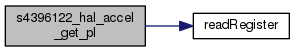
\includegraphics[width=293pt]{d6/d4a/s4396122__hal__accel_8h_a7c6ddaf7d43db64f178bcf2f416d4ad6_cgraph}
\end{center}
\end{figure}



\hypertarget{s4396122__hal__hamming_8c}{}\section{mylib/s4396122\+\_\+hal\+\_\+hamming.c File Reference}
\label{s4396122__hal__hamming_8c}\index{mylib/s4396122\+\_\+hal\+\_\+hamming.\+c@{mylib/s4396122\+\_\+hal\+\_\+hamming.\+c}}


Library for encoding and decoding of hamming codes.  


{\ttfamily \#include \char`\"{}s4396122\+\_\+hal\+\_\+hamming.\+h\char`\"{}}\\*
Include dependency graph for s4396122\+\_\+hal\+\_\+hamming.\+c\+:\nopagebreak
\begin{figure}[H]
\begin{center}
\leavevmode
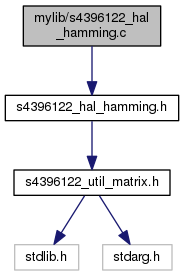
\includegraphics[width=210pt]{d9/de5/s4396122__hal__hamming_8c__incl}
\end{center}
\end{figure}
\subsection*{Functions}
\begin{DoxyCompactItemize}
\item 
int \hyperlink{s4396122__hal__hamming_8c_ae47065534a17887b005d74d2308a1192}{modulate\+\_\+matrix} (int in)
\begin{DoxyCompactList}\small\item\em To be executed from within a matrix, applies mod 2 to every element in the matrix. \end{DoxyCompactList}\item 
void \hyperlink{s4396122__hal__hamming_8c_a762a36d0dbdeb6574f24f8b52ac33cbd}{s4396122\+\_\+hal\+\_\+hamming\+\_\+init} ()\hypertarget{s4396122__hal__hamming_8c_a762a36d0dbdeb6574f24f8b52ac33cbd}{}\label{s4396122__hal__hamming_8c_a762a36d0dbdeb6574f24f8b52ac33cbd}

\begin{DoxyCompactList}\small\item\em Initializes the Generator and Hamming matrix into memory for quick and easy access later. \end{DoxyCompactList}\item 
unsigned int \hyperlink{s4396122__hal__hamming_8c_a871d8329fa2b4bcc418acb7e0ecde547}{s4396122\+\_\+hal\+\_\+hamming\+\_\+encode} (unsigned int in)
\begin{DoxyCompactList}\small\item\em Encodes one nibble of data and returns the hamming encoded nibble. \end{DoxyCompactList}\item 
unsigned int \hyperlink{s4396122__hal__hamming_8c_ae0aac21fb3c2577bb3f945fddccc967d}{s4396122\+\_\+hal\+\_\+hamming\+\_\+decode} (unsigned int in)
\begin{DoxyCompactList}\small\item\em Decodes one nibble of data and returns the data corrected data if any one bit errors exist. \end{DoxyCompactList}\end{DoxyCompactItemize}


\subsection{Detailed Description}
Library for encoding and decoding of hamming codes. 

\begin{DoxyAuthor}{Author}
Daniel Fitzmaurice -\/ 43961229 
\end{DoxyAuthor}
\begin{DoxyVersion}{Version}
1 
\end{DoxyVersion}
\begin{DoxyDate}{Date}
2017-\/05-\/31 
\end{DoxyDate}


\subsection{Function Documentation}
\index{s4396122\+\_\+hal\+\_\+hamming.\+c@{s4396122\+\_\+hal\+\_\+hamming.\+c}!modulate\+\_\+matrix@{modulate\+\_\+matrix}}
\index{modulate\+\_\+matrix@{modulate\+\_\+matrix}!s4396122\+\_\+hal\+\_\+hamming.\+c@{s4396122\+\_\+hal\+\_\+hamming.\+c}}
\subsubsection[{\texorpdfstring{modulate\+\_\+matrix(int in)}{modulate_matrix(int in)}}]{\setlength{\rightskip}{0pt plus 5cm}int modulate\+\_\+matrix (
\begin{DoxyParamCaption}
\item[{int}]{in}
\end{DoxyParamCaption}
)}\hypertarget{s4396122__hal__hamming_8c_ae47065534a17887b005d74d2308a1192}{}\label{s4396122__hal__hamming_8c_ae47065534a17887b005d74d2308a1192}


To be executed from within a matrix, applies mod 2 to every element in the matrix. 


\begin{DoxyParams}{Parameters}
{\em in} & The current value in the matrix \\
\hline
\end{DoxyParams}
\begin{DoxyReturn}{Returns}
The new value in the matrix 
\end{DoxyReturn}
\index{s4396122\+\_\+hal\+\_\+hamming.\+c@{s4396122\+\_\+hal\+\_\+hamming.\+c}!s4396122\+\_\+hal\+\_\+hamming\+\_\+decode@{s4396122\+\_\+hal\+\_\+hamming\+\_\+decode}}
\index{s4396122\+\_\+hal\+\_\+hamming\+\_\+decode@{s4396122\+\_\+hal\+\_\+hamming\+\_\+decode}!s4396122\+\_\+hal\+\_\+hamming.\+c@{s4396122\+\_\+hal\+\_\+hamming.\+c}}
\subsubsection[{\texorpdfstring{s4396122\+\_\+hal\+\_\+hamming\+\_\+decode(unsigned int in)}{s4396122_hal_hamming_decode(unsigned int in)}}]{\setlength{\rightskip}{0pt plus 5cm}unsigned int s4396122\+\_\+hal\+\_\+hamming\+\_\+decode (
\begin{DoxyParamCaption}
\item[{unsigned int}]{in}
\end{DoxyParamCaption}
)}\hypertarget{s4396122__hal__hamming_8c_ae0aac21fb3c2577bb3f945fddccc967d}{}\label{s4396122__hal__hamming_8c_ae0aac21fb3c2577bb3f945fddccc967d}


Decodes one nibble of data and returns the data corrected data if any one bit errors exist. 


\begin{DoxyParams}{Parameters}
{\em in} & Hamming encoded data \\
\hline
\end{DoxyParams}
\begin{DoxyReturn}{Returns}
The decoded data with any error corrections. If there is 2 errors then 0x\+FF is returned 
\end{DoxyReturn}


Here is the call graph for this function\+:\nopagebreak
\begin{figure}[H]
\begin{center}
\leavevmode
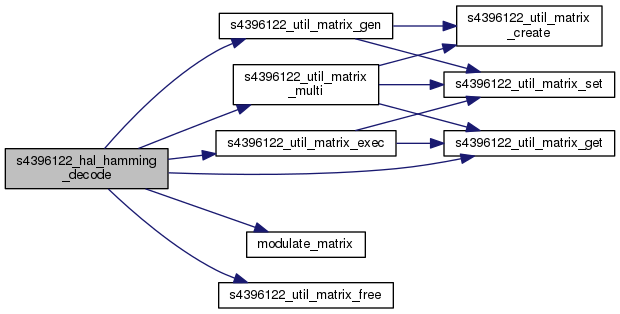
\includegraphics[width=350pt]{d3/d4a/s4396122__hal__hamming_8c_ae0aac21fb3c2577bb3f945fddccc967d_cgraph}
\end{center}
\end{figure}


\index{s4396122\+\_\+hal\+\_\+hamming.\+c@{s4396122\+\_\+hal\+\_\+hamming.\+c}!s4396122\+\_\+hal\+\_\+hamming\+\_\+encode@{s4396122\+\_\+hal\+\_\+hamming\+\_\+encode}}
\index{s4396122\+\_\+hal\+\_\+hamming\+\_\+encode@{s4396122\+\_\+hal\+\_\+hamming\+\_\+encode}!s4396122\+\_\+hal\+\_\+hamming.\+c@{s4396122\+\_\+hal\+\_\+hamming.\+c}}
\subsubsection[{\texorpdfstring{s4396122\+\_\+hal\+\_\+hamming\+\_\+encode(unsigned int in)}{s4396122_hal_hamming_encode(unsigned int in)}}]{\setlength{\rightskip}{0pt plus 5cm}unsigned int s4396122\+\_\+hal\+\_\+hamming\+\_\+encode (
\begin{DoxyParamCaption}
\item[{unsigned int}]{in}
\end{DoxyParamCaption}
)}\hypertarget{s4396122__hal__hamming_8c_a871d8329fa2b4bcc418acb7e0ecde547}{}\label{s4396122__hal__hamming_8c_a871d8329fa2b4bcc418acb7e0ecde547}


Encodes one nibble of data and returns the hamming encoded nibble. 


\begin{DoxyParams}{Parameters}
{\em in} & Nibble to be encoded \\
\hline
\end{DoxyParams}
\begin{DoxyReturn}{Returns}
Encoded nibble of data 
\end{DoxyReturn}


Here is the call graph for this function\+:\nopagebreak
\begin{figure}[H]
\begin{center}
\leavevmode
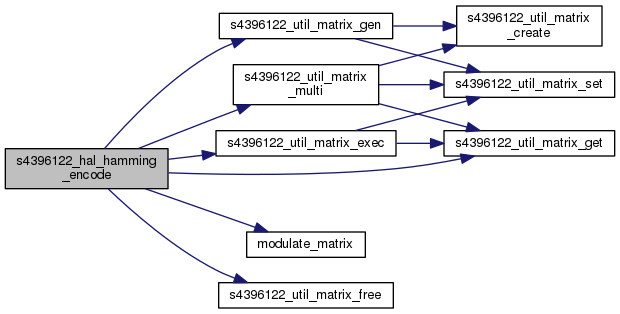
\includegraphics[width=350pt]{d3/d4a/s4396122__hal__hamming_8c_a871d8329fa2b4bcc418acb7e0ecde547_cgraph}
\end{center}
\end{figure}



\hypertarget{s4396122__hal__hamming_8h}{}\section{mylib/s4396122\+\_\+hal\+\_\+hamming.h File Reference}
\label{s4396122__hal__hamming_8h}\index{mylib/s4396122\+\_\+hal\+\_\+hamming.\+h@{mylib/s4396122\+\_\+hal\+\_\+hamming.\+h}}


Library for encoding and decoding of hamming codes.  


{\ttfamily \#include \char`\"{}s4396122\+\_\+util\+\_\+matrix.\+h\char`\"{}}\\*
Include dependency graph for s4396122\+\_\+hal\+\_\+hamming.\+h\+:\nopagebreak
\begin{figure}[H]
\begin{center}
\leavevmode
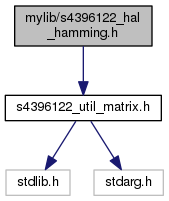
\includegraphics[width=199pt]{dc/d03/s4396122__hal__hamming_8h__incl}
\end{center}
\end{figure}
This graph shows which files directly or indirectly include this file\+:\nopagebreak
\begin{figure}[H]
\begin{center}
\leavevmode
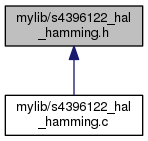
\includegraphics[width=183pt]{d2/da9/s4396122__hal__hamming_8h__dep__incl}
\end{center}
\end{figure}
\subsection*{Functions}
\begin{DoxyCompactItemize}
\item 
void \hyperlink{s4396122__hal__hamming_8h_a762a36d0dbdeb6574f24f8b52ac33cbd}{s4396122\+\_\+hal\+\_\+hamming\+\_\+init} ()\hypertarget{s4396122__hal__hamming_8h_a762a36d0dbdeb6574f24f8b52ac33cbd}{}\label{s4396122__hal__hamming_8h_a762a36d0dbdeb6574f24f8b52ac33cbd}

\begin{DoxyCompactList}\small\item\em Initializes the Generator and Hamming matrix into memory for quick and easy access later. \end{DoxyCompactList}\item 
unsigned int \hyperlink{s4396122__hal__hamming_8h_a871d8329fa2b4bcc418acb7e0ecde547}{s4396122\+\_\+hal\+\_\+hamming\+\_\+encode} (unsigned int in)
\begin{DoxyCompactList}\small\item\em Encodes one nibble of data and returns the hamming encoded nibble. \end{DoxyCompactList}\item 
unsigned int \hyperlink{s4396122__hal__hamming_8h_ae0aac21fb3c2577bb3f945fddccc967d}{s4396122\+\_\+hal\+\_\+hamming\+\_\+decode} (unsigned int in)
\begin{DoxyCompactList}\small\item\em Decodes one nibble of data and returns the data corrected data if any one bit errors exist. \end{DoxyCompactList}\end{DoxyCompactItemize}
\subsection*{Variables}
\begin{DoxyCompactItemize}
\item 
\hyperlink{structMatrix}{Matrix} $\ast$ \hyperlink{s4396122__hal__hamming_8h_aa08cc6ac70b1cf2ecb03802ef0d0325d}{G\+Encoder}\hypertarget{s4396122__hal__hamming_8h_aa08cc6ac70b1cf2ecb03802ef0d0325d}{}\label{s4396122__hal__hamming_8h_aa08cc6ac70b1cf2ecb03802ef0d0325d}

\begin{DoxyCompactList}\small\item\em \hyperlink{structMatrix}{Matrix} containing the G encoding. \end{DoxyCompactList}\item 
\hyperlink{structMatrix}{Matrix} $\ast$ \hyperlink{s4396122__hal__hamming_8h_a93f22af89671b4709be33b7ea81a01e0}{H\+Decoder}\hypertarget{s4396122__hal__hamming_8h_a93f22af89671b4709be33b7ea81a01e0}{}\label{s4396122__hal__hamming_8h_a93f22af89671b4709be33b7ea81a01e0}

\begin{DoxyCompactList}\small\item\em \hyperlink{structMatrix}{Matrix} containing the H decoding. \end{DoxyCompactList}\end{DoxyCompactItemize}


\subsection{Detailed Description}
Library for encoding and decoding of hamming codes. 

\begin{DoxyAuthor}{Author}
Daniel Fitzmaurice -\/ 43961229 
\end{DoxyAuthor}
\begin{DoxyVersion}{Version}
1 
\end{DoxyVersion}
\begin{DoxyDate}{Date}
2017-\/05-\/31 
\end{DoxyDate}


\subsection{Function Documentation}
\index{s4396122\+\_\+hal\+\_\+hamming.\+h@{s4396122\+\_\+hal\+\_\+hamming.\+h}!s4396122\+\_\+hal\+\_\+hamming\+\_\+decode@{s4396122\+\_\+hal\+\_\+hamming\+\_\+decode}}
\index{s4396122\+\_\+hal\+\_\+hamming\+\_\+decode@{s4396122\+\_\+hal\+\_\+hamming\+\_\+decode}!s4396122\+\_\+hal\+\_\+hamming.\+h@{s4396122\+\_\+hal\+\_\+hamming.\+h}}
\subsubsection[{\texorpdfstring{s4396122\+\_\+hal\+\_\+hamming\+\_\+decode(unsigned int in)}{s4396122_hal_hamming_decode(unsigned int in)}}]{\setlength{\rightskip}{0pt plus 5cm}unsigned int s4396122\+\_\+hal\+\_\+hamming\+\_\+decode (
\begin{DoxyParamCaption}
\item[{unsigned int}]{in}
\end{DoxyParamCaption}
)}\hypertarget{s4396122__hal__hamming_8h_ae0aac21fb3c2577bb3f945fddccc967d}{}\label{s4396122__hal__hamming_8h_ae0aac21fb3c2577bb3f945fddccc967d}


Decodes one nibble of data and returns the data corrected data if any one bit errors exist. 


\begin{DoxyParams}{Parameters}
{\em in} & Hamming encoded data \\
\hline
\end{DoxyParams}
\begin{DoxyReturn}{Returns}
The decoded data with any error corrections. If there is 2 errors then 0x\+FF is returned 
\end{DoxyReturn}


Here is the call graph for this function\+:\nopagebreak
\begin{figure}[H]
\begin{center}
\leavevmode
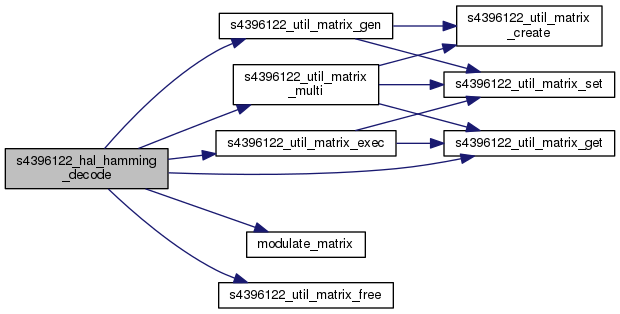
\includegraphics[width=350pt]{db/d9b/s4396122__hal__hamming_8h_ae0aac21fb3c2577bb3f945fddccc967d_cgraph}
\end{center}
\end{figure}


\index{s4396122\+\_\+hal\+\_\+hamming.\+h@{s4396122\+\_\+hal\+\_\+hamming.\+h}!s4396122\+\_\+hal\+\_\+hamming\+\_\+encode@{s4396122\+\_\+hal\+\_\+hamming\+\_\+encode}}
\index{s4396122\+\_\+hal\+\_\+hamming\+\_\+encode@{s4396122\+\_\+hal\+\_\+hamming\+\_\+encode}!s4396122\+\_\+hal\+\_\+hamming.\+h@{s4396122\+\_\+hal\+\_\+hamming.\+h}}
\subsubsection[{\texorpdfstring{s4396122\+\_\+hal\+\_\+hamming\+\_\+encode(unsigned int in)}{s4396122_hal_hamming_encode(unsigned int in)}}]{\setlength{\rightskip}{0pt plus 5cm}unsigned int s4396122\+\_\+hal\+\_\+hamming\+\_\+encode (
\begin{DoxyParamCaption}
\item[{unsigned int}]{in}
\end{DoxyParamCaption}
)}\hypertarget{s4396122__hal__hamming_8h_a871d8329fa2b4bcc418acb7e0ecde547}{}\label{s4396122__hal__hamming_8h_a871d8329fa2b4bcc418acb7e0ecde547}


Encodes one nibble of data and returns the hamming encoded nibble. 


\begin{DoxyParams}{Parameters}
{\em in} & Nibble to be encoded \\
\hline
\end{DoxyParams}
\begin{DoxyReturn}{Returns}
Encoded nibble of data 
\end{DoxyReturn}


Here is the call graph for this function\+:\nopagebreak
\begin{figure}[H]
\begin{center}
\leavevmode
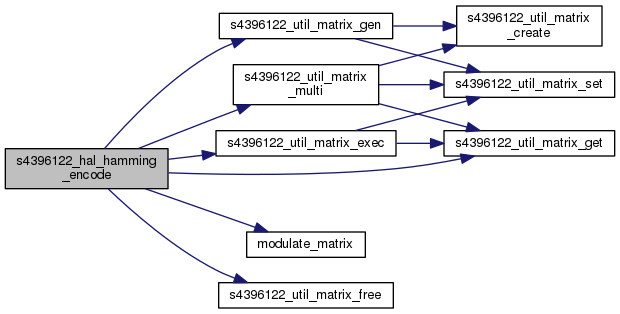
\includegraphics[width=350pt]{db/d9b/s4396122__hal__hamming_8h_a871d8329fa2b4bcc418acb7e0ecde547_cgraph}
\end{center}
\end{figure}



\hypertarget{s4396122__hal__ir_8c}{}\section{mylib/s4396122\+\_\+hal\+\_\+ir.c File Reference}
\label{s4396122__hal__ir_8c}\index{mylib/s4396122\+\_\+hal\+\_\+ir.\+c@{mylib/s4396122\+\_\+hal\+\_\+ir.\+c}}


Control library for the IR transmitter and receiver.  


{\ttfamily \#include \char`\"{}s4396122\+\_\+hal\+\_\+ir.\+h\char`\"{}}\\*
Include dependency graph for s4396122\+\_\+hal\+\_\+ir.\+c\+:\nopagebreak
\begin{figure}[H]
\begin{center}
\leavevmode
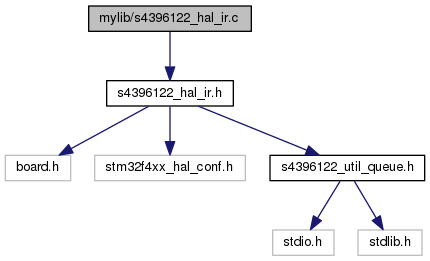
\includegraphics[width=350pt]{d5/d0e/s4396122__hal__ir_8c__incl}
\end{center}
\end{figure}
\subsection*{Functions}
\begin{DoxyCompactItemize}
\item 
void \hyperlink{s4396122__hal__ir_8c_a79383d1eb7a6461c1ee7748a84c6acae}{s4396122\+\_\+hal\+\_\+ir\+\_\+interrupt} ()\hypertarget{s4396122__hal__ir_8c_a79383d1eb7a6461c1ee7748a84c6acae}{}\label{s4396122__hal__ir_8c_a79383d1eb7a6461c1ee7748a84c6acae}

\begin{DoxyCompactList}\small\item\em Handles the interrupt for the ir input. The timings will be stored in a queue for processing later on. \end{DoxyCompactList}\item 
void \hyperlink{s4396122__hal__ir_8c_ad77fb83f56d03670d3365052699eaadb}{s4396122\+\_\+hal\+\_\+ir\+\_\+init} ()\hypertarget{s4396122__hal__ir_8c_ad77fb83f56d03670d3365052699eaadb}{}\label{s4396122__hal__ir_8c_ad77fb83f56d03670d3365052699eaadb}

\begin{DoxyCompactList}\small\item\em Initializes the hardware for the ir transmitter. This will also turn the carrier signal on. Pin D8 is the logic pin and D1 is the carrier signal. \end{DoxyCompactList}\item 
void \hyperlink{s4396122__hal__ir_8c_acf1c32d6e4e958b01b3f2db410b63312}{irhal\+\_\+carrier} (int state)
\begin{DoxyCompactList}\small\item\em Turns on or off the carrier signal. \end{DoxyCompactList}\item 
\hyperlink{structQueue}{Queue} $\ast$ \hyperlink{s4396122__hal__ir_8c_a32206e24b83574e02595e1edc1132db1}{s4396122\+\_\+hal\+\_\+ir\+\_\+get\+\_\+queue} ()
\begin{DoxyCompactList}\small\item\em Gets the I\+R\+Queue and returns it for referencing to external libraries and functions. \end{DoxyCompactList}\end{DoxyCompactItemize}
\subsection*{Variables}
\begin{DoxyCompactItemize}
\item 
T\+I\+M\+\_\+\+Handle\+Type\+Def \hyperlink{s4396122__hal__ir_8c_a0b2cba495b01a94a7df3e44146dd9468}{T\+I\+M\+\_\+\+Init}\hypertarget{s4396122__hal__ir_8c_a0b2cba495b01a94a7df3e44146dd9468}{}\label{s4396122__hal__ir_8c_a0b2cba495b01a94a7df3e44146dd9468}

\begin{DoxyCompactList}\small\item\em Local definition of modulation wave timer. \end{DoxyCompactList}\item 
T\+I\+M\+\_\+\+Handle\+Type\+Def \hyperlink{s4396122__hal__ir_8c_a171a80a903e9c2af570c876421cb205b}{I\+R\+\_\+\+Input\+\_\+\+Init}\hypertarget{s4396122__hal__ir_8c_a171a80a903e9c2af570c876421cb205b}{}\label{s4396122__hal__ir_8c_a171a80a903e9c2af570c876421cb205b}

\begin{DoxyCompactList}\small\item\em Keep as a local definition. \end{DoxyCompactList}\end{DoxyCompactItemize}


\subsection{Detailed Description}
Control library for the IR transmitter and receiver. 

\begin{DoxyAuthor}{Author}
Daniel Fitzmaurice -\/ 43961229 
\end{DoxyAuthor}
\begin{DoxyVersion}{Version}
1 
\end{DoxyVersion}
\begin{DoxyDate}{Date}
2017-\/05-\/31 
\end{DoxyDate}


\subsection{Function Documentation}
\index{s4396122\+\_\+hal\+\_\+ir.\+c@{s4396122\+\_\+hal\+\_\+ir.\+c}!irhal\+\_\+carrier@{irhal\+\_\+carrier}}
\index{irhal\+\_\+carrier@{irhal\+\_\+carrier}!s4396122\+\_\+hal\+\_\+ir.\+c@{s4396122\+\_\+hal\+\_\+ir.\+c}}
\subsubsection[{\texorpdfstring{irhal\+\_\+carrier(int state)}{irhal_carrier(int state)}}]{\setlength{\rightskip}{0pt plus 5cm}void irhal\+\_\+carrier (
\begin{DoxyParamCaption}
\item[{int}]{state}
\end{DoxyParamCaption}
)}\hypertarget{s4396122__hal__ir_8c_acf1c32d6e4e958b01b3f2db410b63312}{}\label{s4396122__hal__ir_8c_acf1c32d6e4e958b01b3f2db410b63312}


Turns on or off the carrier signal. 


\begin{DoxyParams}{Parameters}
{\em state} & (1 = turns on the signal), (0 = turns off the signal) \\
\hline
\end{DoxyParams}
\index{s4396122\+\_\+hal\+\_\+ir.\+c@{s4396122\+\_\+hal\+\_\+ir.\+c}!s4396122\+\_\+hal\+\_\+ir\+\_\+get\+\_\+queue@{s4396122\+\_\+hal\+\_\+ir\+\_\+get\+\_\+queue}}
\index{s4396122\+\_\+hal\+\_\+ir\+\_\+get\+\_\+queue@{s4396122\+\_\+hal\+\_\+ir\+\_\+get\+\_\+queue}!s4396122\+\_\+hal\+\_\+ir.\+c@{s4396122\+\_\+hal\+\_\+ir.\+c}}
\subsubsection[{\texorpdfstring{s4396122\+\_\+hal\+\_\+ir\+\_\+get\+\_\+queue()}{s4396122_hal_ir_get_queue()}}]{\setlength{\rightskip}{0pt plus 5cm}{\bf Queue}$\ast$ s4396122\+\_\+hal\+\_\+ir\+\_\+get\+\_\+queue (
\begin{DoxyParamCaption}
{}
\end{DoxyParamCaption}
)}\hypertarget{s4396122__hal__ir_8c_a32206e24b83574e02595e1edc1132db1}{}\label{s4396122__hal__ir_8c_a32206e24b83574e02595e1edc1132db1}


Gets the I\+R\+Queue and returns it for referencing to external libraries and functions. 

\begin{DoxyReturn}{Returns}
The I\+R\+Queue which contains all the current IR data 
\end{DoxyReturn}

\hypertarget{s4396122__hal__ir_8h}{}\section{mylib/s4396122\+\_\+hal\+\_\+ir.h File Reference}
\label{s4396122__hal__ir_8h}\index{mylib/s4396122\+\_\+hal\+\_\+ir.\+h@{mylib/s4396122\+\_\+hal\+\_\+ir.\+h}}


Control library for the IR transmitter and receiver.  


{\ttfamily \#include $<$board.\+h$>$}\\*
{\ttfamily \#include $<$stm32f4xx\+\_\+hal\+\_\+conf.\+h$>$}\\*
{\ttfamily \#include \char`\"{}s4396122\+\_\+util\+\_\+queue.\+h\char`\"{}}\\*
Include dependency graph for s4396122\+\_\+hal\+\_\+ir.\+h\+:\nopagebreak
\begin{figure}[H]
\begin{center}
\leavevmode
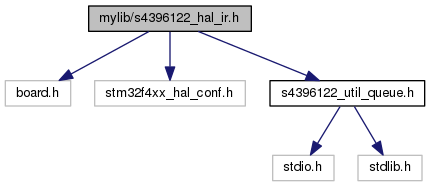
\includegraphics[width=350pt]{dd/d55/s4396122__hal__ir_8h__incl}
\end{center}
\end{figure}
This graph shows which files directly or indirectly include this file\+:\nopagebreak
\begin{figure}[H]
\begin{center}
\leavevmode
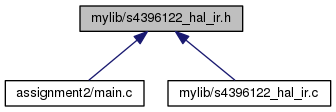
\includegraphics[width=324pt]{d4/dd6/s4396122__hal__ir_8h__dep__incl}
\end{center}
\end{figure}
\subsection*{Macros}
\begin{DoxyCompactItemize}
\item 
\#define \hyperlink{s4396122__hal__ir_8h_ac204c66fe38e31f6c97cb3e55bf855a1}{s4396122\+\_\+hal\+\_\+ir\+\_\+carrieron}()~\hyperlink{s4396122__hal__ir_8h_acf1c32d6e4e958b01b3f2db410b63312}{irhal\+\_\+carrier}(1);\hypertarget{s4396122__hal__ir_8h_ac204c66fe38e31f6c97cb3e55bf855a1}{}\label{s4396122__hal__ir_8h_ac204c66fe38e31f6c97cb3e55bf855a1}

\begin{DoxyCompactList}\small\item\em Enables the ir carrier signal. \end{DoxyCompactList}\item 
\#define \hyperlink{s4396122__hal__ir_8h_af0d86b14938113b4b4f34854ae5daa77}{s4396122\+\_\+hal\+\_\+ir\+\_\+carrieroff}()~\hyperlink{s4396122__hal__ir_8h_acf1c32d6e4e958b01b3f2db410b63312}{irhal\+\_\+carrier}(0);\hypertarget{s4396122__hal__ir_8h_af0d86b14938113b4b4f34854ae5daa77}{}\label{s4396122__hal__ir_8h_af0d86b14938113b4b4f34854ae5daa77}

\begin{DoxyCompactList}\small\item\em Disables the ir carrier signal. \end{DoxyCompactList}\item 
\#define \hyperlink{s4396122__hal__ir_8h_a383244214b904e714ae4cb593f148928}{s4396122\+\_\+hal\+\_\+ir\+\_\+datamodulation\+\_\+set}()~H\+A\+L\+\_\+\+G\+P\+I\+O\+\_\+\+Write\+Pin(B\+R\+D\+\_\+\+D8\+\_\+\+G\+P\+I\+O\+\_\+\+P\+O\+RT, B\+R\+D\+\_\+\+D8\+\_\+\+P\+IN, 1);\hypertarget{s4396122__hal__ir_8h_a383244214b904e714ae4cb593f148928}{}\label{s4396122__hal__ir_8h_a383244214b904e714ae4cb593f148928}

\begin{DoxyCompactList}\small\item\em Sets the ir output to high. \end{DoxyCompactList}\item 
\#define \hyperlink{s4396122__hal__ir_8h_ab980c052ef97ebbc8cd3a624c0f14a53}{s4396122\+\_\+hal\+\_\+ir\+\_\+datamodulation\+\_\+cli}()~H\+A\+L\+\_\+\+G\+P\+I\+O\+\_\+\+Write\+Pin(B\+R\+D\+\_\+\+D8\+\_\+\+G\+P\+I\+O\+\_\+\+P\+O\+RT, B\+R\+D\+\_\+\+D8\+\_\+\+P\+IN, 0);\hypertarget{s4396122__hal__ir_8h_ab980c052ef97ebbc8cd3a624c0f14a53}{}\label{s4396122__hal__ir_8h_ab980c052ef97ebbc8cd3a624c0f14a53}

\begin{DoxyCompactList}\small\item\em Sets the ir output to low. \end{DoxyCompactList}\end{DoxyCompactItemize}
\subsection*{Functions}
\begin{DoxyCompactItemize}
\item 
void \hyperlink{s4396122__hal__ir_8h_ad77fb83f56d03670d3365052699eaadb}{s4396122\+\_\+hal\+\_\+ir\+\_\+init} ()\hypertarget{s4396122__hal__ir_8h_ad77fb83f56d03670d3365052699eaadb}{}\label{s4396122__hal__ir_8h_ad77fb83f56d03670d3365052699eaadb}

\begin{DoxyCompactList}\small\item\em Initializes the hardware for the ir transmitter. This will also turn the carrier signal on. Pin D8 is the logic pin and D1 is the carrier signal. \end{DoxyCompactList}\item 
void \hyperlink{s4396122__hal__ir_8h_acf1c32d6e4e958b01b3f2db410b63312}{irhal\+\_\+carrier} (int state)
\begin{DoxyCompactList}\small\item\em Turns on or off the carrier signal. \end{DoxyCompactList}\item 
\hyperlink{structQueue}{Queue} $\ast$ \hyperlink{s4396122__hal__ir_8h_a32206e24b83574e02595e1edc1132db1}{s4396122\+\_\+hal\+\_\+ir\+\_\+get\+\_\+queue} ()
\begin{DoxyCompactList}\small\item\em Gets the I\+R\+Queue and returns it for referencing to external libraries and functions. \end{DoxyCompactList}\end{DoxyCompactItemize}
\subsection*{Variables}
\begin{DoxyCompactItemize}
\item 
\hyperlink{structQueue}{Queue} $\ast$ \hyperlink{s4396122__hal__ir_8h_a3df1ce450db429c97f247271d0a8e6cb}{I\+R\+Queue}\hypertarget{s4396122__hal__ir_8h_a3df1ce450db429c97f247271d0a8e6cb}{}\label{s4396122__hal__ir_8h_a3df1ce450db429c97f247271d0a8e6cb}

\begin{DoxyCompactList}\small\item\em Global variable for storing and accessing the IR data. \end{DoxyCompactList}\end{DoxyCompactItemize}


\subsection{Detailed Description}
Control library for the IR transmitter and receiver. 

\begin{DoxyAuthor}{Author}
Daniel Fitzmaurice -\/ 43961229 
\end{DoxyAuthor}
\begin{DoxyVersion}{Version}
1 
\end{DoxyVersion}
\begin{DoxyDate}{Date}
2017-\/05-\/31 
\end{DoxyDate}


\subsection{Function Documentation}
\index{s4396122\+\_\+hal\+\_\+ir.\+h@{s4396122\+\_\+hal\+\_\+ir.\+h}!irhal\+\_\+carrier@{irhal\+\_\+carrier}}
\index{irhal\+\_\+carrier@{irhal\+\_\+carrier}!s4396122\+\_\+hal\+\_\+ir.\+h@{s4396122\+\_\+hal\+\_\+ir.\+h}}
\subsubsection[{\texorpdfstring{irhal\+\_\+carrier(int state)}{irhal_carrier(int state)}}]{\setlength{\rightskip}{0pt plus 5cm}void irhal\+\_\+carrier (
\begin{DoxyParamCaption}
\item[{int}]{state}
\end{DoxyParamCaption}
)}\hypertarget{s4396122__hal__ir_8h_acf1c32d6e4e958b01b3f2db410b63312}{}\label{s4396122__hal__ir_8h_acf1c32d6e4e958b01b3f2db410b63312}


Turns on or off the carrier signal. 


\begin{DoxyParams}{Parameters}
{\em state} & (1 = turns on the signal), (0 = turns off the signal) \\
\hline
\end{DoxyParams}
\index{s4396122\+\_\+hal\+\_\+ir.\+h@{s4396122\+\_\+hal\+\_\+ir.\+h}!s4396122\+\_\+hal\+\_\+ir\+\_\+get\+\_\+queue@{s4396122\+\_\+hal\+\_\+ir\+\_\+get\+\_\+queue}}
\index{s4396122\+\_\+hal\+\_\+ir\+\_\+get\+\_\+queue@{s4396122\+\_\+hal\+\_\+ir\+\_\+get\+\_\+queue}!s4396122\+\_\+hal\+\_\+ir.\+h@{s4396122\+\_\+hal\+\_\+ir.\+h}}
\subsubsection[{\texorpdfstring{s4396122\+\_\+hal\+\_\+ir\+\_\+get\+\_\+queue()}{s4396122_hal_ir_get_queue()}}]{\setlength{\rightskip}{0pt plus 5cm}{\bf Queue}$\ast$ s4396122\+\_\+hal\+\_\+ir\+\_\+get\+\_\+queue (
\begin{DoxyParamCaption}
{}
\end{DoxyParamCaption}
)}\hypertarget{s4396122__hal__ir_8h_a32206e24b83574e02595e1edc1132db1}{}\label{s4396122__hal__ir_8h_a32206e24b83574e02595e1edc1132db1}


Gets the I\+R\+Queue and returns it for referencing to external libraries and functions. 

\begin{DoxyReturn}{Returns}
The I\+R\+Queue which contains all the current IR data 
\end{DoxyReturn}

\hypertarget{s4396122__hal__ircoms_8c}{}\section{mylib/s4396122\+\_\+hal\+\_\+ircoms.c File Reference}
\label{s4396122__hal__ircoms_8c}\index{mylib/s4396122\+\_\+hal\+\_\+ircoms.\+c@{mylib/s4396122\+\_\+hal\+\_\+ircoms.\+c}}


Library for encoding and decoding of data to manchester waveforms.  


{\ttfamily \#include \char`\"{}s4396122\+\_\+hal\+\_\+ircoms.\+h\char`\"{}}\\*
Include dependency graph for s4396122\+\_\+hal\+\_\+ircoms.\+c\+:\nopagebreak
\begin{figure}[H]
\begin{center}
\leavevmode
\includegraphics[width=199pt]{dd/d4d/s4396122__hal__ircoms_8c__incl}
\end{center}
\end{figure}
\subsection*{Functions}
\begin{DoxyCompactItemize}
\item 
void \hyperlink{s4396122__hal__ircoms_8c_af6db5d5da986be74c8d4f49a30df2acd}{manchester\+\_\+encode} (\hyperlink{structQueue}{Queue} $\ast$q, unsigned int bit)
\begin{DoxyCompactList}\small\item\em Encodes a bit into a \hyperlink{structQueue}{Queue}. \end{DoxyCompactList}\item 
\hyperlink{structQueue}{Queue} $\ast$ \hyperlink{s4396122__hal__ircoms_8c_af335092b42755a4eb0a17bf29e496d54}{s4396122\+\_\+hal\+\_\+ircoms\+\_\+encode} (unsigned int hamming\+Code)
\begin{DoxyCompactList}\small\item\em Encodes a byte of data into a \hyperlink{structQueue}{Queue} of manchester waveform. \end{DoxyCompactList}\item 
int \hyperlink{s4396122__hal__ircoms_8c_a4f68da46bb9058a63a6b1cc238ca3743}{manchester\+\_\+decode} (\hyperlink{structQueue}{Queue} $\ast$in\+Queue)
\begin{DoxyCompactList}\small\item\em Decodes one group of bits and returns the result. \end{DoxyCompactList}\item 
unsigned int \hyperlink{s4396122__hal__ircoms_8c_ad0c503052637583ddd3ac840d9e4791a}{s4396122\+\_\+hal\+\_\+ircoms\+\_\+decode} (\hyperlink{structQueue}{Queue} $\ast$in\+Queue)
\begin{DoxyCompactList}\small\item\em Decodes a \hyperlink{structQueue}{Queue} of manchester bits and returns an int of the decoded \hyperlink{structQueue}{Queue}. \end{DoxyCompactList}\end{DoxyCompactItemize}


\subsection{Detailed Description}
Library for encoding and decoding of data to manchester waveforms. 

\begin{DoxyAuthor}{Author}
Daniel Fitzmaurice -\/ 43961229 
\end{DoxyAuthor}
\begin{DoxyVersion}{Version}
1 
\end{DoxyVersion}
\begin{DoxyDate}{Date}
2017-\/05-\/31 
\end{DoxyDate}


\subsection{Function Documentation}
\index{s4396122\+\_\+hal\+\_\+ircoms.\+c@{s4396122\+\_\+hal\+\_\+ircoms.\+c}!manchester\+\_\+decode@{manchester\+\_\+decode}}
\index{manchester\+\_\+decode@{manchester\+\_\+decode}!s4396122\+\_\+hal\+\_\+ircoms.\+c@{s4396122\+\_\+hal\+\_\+ircoms.\+c}}
\subsubsection[{\texorpdfstring{manchester\+\_\+decode(\+Queue $\ast$in\+Queue)}{manchester_decode(Queue *inQueue)}}]{\setlength{\rightskip}{0pt plus 5cm}int manchester\+\_\+decode (
\begin{DoxyParamCaption}
\item[{{\bf Queue} $\ast$}]{in\+Queue}
\end{DoxyParamCaption}
)}\hypertarget{s4396122__hal__ircoms_8c_a4f68da46bb9058a63a6b1cc238ca3743}{}\label{s4396122__hal__ircoms_8c_a4f68da46bb9058a63a6b1cc238ca3743}


Decodes one group of bits and returns the result. 


\begin{DoxyParams}{Parameters}
{\em in\+Queue} & \hyperlink{structQueue}{Queue} to extract bits from \\
\hline
\end{DoxyParams}
\begin{DoxyReturn}{Returns}
Either 1 or 0 based on the bits decoded 
\end{DoxyReturn}


Here is the call graph for this function\+:\nopagebreak
\begin{figure}[H]
\begin{center}
\leavevmode
\includegraphics[width=349pt]{d0/da1/s4396122__hal__ircoms_8c_a4f68da46bb9058a63a6b1cc238ca3743_cgraph}
\end{center}
\end{figure}


\index{s4396122\+\_\+hal\+\_\+ircoms.\+c@{s4396122\+\_\+hal\+\_\+ircoms.\+c}!manchester\+\_\+encode@{manchester\+\_\+encode}}
\index{manchester\+\_\+encode@{manchester\+\_\+encode}!s4396122\+\_\+hal\+\_\+ircoms.\+c@{s4396122\+\_\+hal\+\_\+ircoms.\+c}}
\subsubsection[{\texorpdfstring{manchester\+\_\+encode(\+Queue $\ast$q, unsigned int bit)}{manchester_encode(Queue *q, unsigned int bit)}}]{\setlength{\rightskip}{0pt plus 5cm}void manchester\+\_\+encode (
\begin{DoxyParamCaption}
\item[{{\bf Queue} $\ast$}]{q, }
\item[{unsigned int}]{bit}
\end{DoxyParamCaption}
)}\hypertarget{s4396122__hal__ircoms_8c_af6db5d5da986be74c8d4f49a30df2acd}{}\label{s4396122__hal__ircoms_8c_af6db5d5da986be74c8d4f49a30df2acd}


Encodes a bit into a \hyperlink{structQueue}{Queue}. 


\begin{DoxyParams}{Parameters}
{\em q} & \hyperlink{structQueue}{Queue} to add the encoded bit to \\
\hline
{\em bit} & Bit to be encoded \\
\hline
\end{DoxyParams}


Here is the call graph for this function\+:\nopagebreak
\begin{figure}[H]
\begin{center}
\leavevmode
\includegraphics[width=350pt]{d0/da1/s4396122__hal__ircoms_8c_af6db5d5da986be74c8d4f49a30df2acd_cgraph}
\end{center}
\end{figure}


\index{s4396122\+\_\+hal\+\_\+ircoms.\+c@{s4396122\+\_\+hal\+\_\+ircoms.\+c}!s4396122\+\_\+hal\+\_\+ircoms\+\_\+decode@{s4396122\+\_\+hal\+\_\+ircoms\+\_\+decode}}
\index{s4396122\+\_\+hal\+\_\+ircoms\+\_\+decode@{s4396122\+\_\+hal\+\_\+ircoms\+\_\+decode}!s4396122\+\_\+hal\+\_\+ircoms.\+c@{s4396122\+\_\+hal\+\_\+ircoms.\+c}}
\subsubsection[{\texorpdfstring{s4396122\+\_\+hal\+\_\+ircoms\+\_\+decode(\+Queue $\ast$in\+Queue)}{s4396122_hal_ircoms_decode(Queue *inQueue)}}]{\setlength{\rightskip}{0pt plus 5cm}unsigned int s4396122\+\_\+hal\+\_\+ircoms\+\_\+decode (
\begin{DoxyParamCaption}
\item[{{\bf Queue} $\ast$}]{in\+Queue}
\end{DoxyParamCaption}
)}\hypertarget{s4396122__hal__ircoms_8c_ad0c503052637583ddd3ac840d9e4791a}{}\label{s4396122__hal__ircoms_8c_ad0c503052637583ddd3ac840d9e4791a}


Decodes a \hyperlink{structQueue}{Queue} of manchester bits and returns an int of the decoded \hyperlink{structQueue}{Queue}. 


\begin{DoxyParams}{Parameters}
{\em in\+Queue} & \hyperlink{structQueue}{Queue} to be decoded \\
\hline
\end{DoxyParams}
\begin{DoxyReturn}{Returns}
Decoded int of the queue 
\end{DoxyReturn}


Here is the call graph for this function\+:\nopagebreak
\begin{figure}[H]
\begin{center}
\leavevmode
\includegraphics[width=350pt]{d0/da1/s4396122__hal__ircoms_8c_ad0c503052637583ddd3ac840d9e4791a_cgraph}
\end{center}
\end{figure}


\index{s4396122\+\_\+hal\+\_\+ircoms.\+c@{s4396122\+\_\+hal\+\_\+ircoms.\+c}!s4396122\+\_\+hal\+\_\+ircoms\+\_\+encode@{s4396122\+\_\+hal\+\_\+ircoms\+\_\+encode}}
\index{s4396122\+\_\+hal\+\_\+ircoms\+\_\+encode@{s4396122\+\_\+hal\+\_\+ircoms\+\_\+encode}!s4396122\+\_\+hal\+\_\+ircoms.\+c@{s4396122\+\_\+hal\+\_\+ircoms.\+c}}
\subsubsection[{\texorpdfstring{s4396122\+\_\+hal\+\_\+ircoms\+\_\+encode(unsigned int hamming\+Code)}{s4396122_hal_ircoms_encode(unsigned int hammingCode)}}]{\setlength{\rightskip}{0pt plus 5cm}{\bf Queue}$\ast$ s4396122\+\_\+hal\+\_\+ircoms\+\_\+encode (
\begin{DoxyParamCaption}
\item[{unsigned int}]{hamming\+Code}
\end{DoxyParamCaption}
)}\hypertarget{s4396122__hal__ircoms_8c_af335092b42755a4eb0a17bf29e496d54}{}\label{s4396122__hal__ircoms_8c_af335092b42755a4eb0a17bf29e496d54}


Encodes a byte of data into a \hyperlink{structQueue}{Queue} of manchester waveform. 


\begin{DoxyParams}{Parameters}
{\em hamming\+Code} & Data to be encoded \\
\hline
\end{DoxyParams}
\begin{DoxyReturn}{Returns}
Resulting \hyperlink{structQueue}{Queue} with manchester coding 
\end{DoxyReturn}


Here is the call graph for this function\+:\nopagebreak
\begin{figure}[H]
\begin{center}
\leavevmode
\includegraphics[width=350pt]{d0/da1/s4396122__hal__ircoms_8c_af335092b42755a4eb0a17bf29e496d54_cgraph}
\end{center}
\end{figure}



\hypertarget{s4396122__hal__ircoms_8h}{}\section{mylib/s4396122\+\_\+hal\+\_\+ircoms.h File Reference}
\label{s4396122__hal__ircoms_8h}\index{mylib/s4396122\+\_\+hal\+\_\+ircoms.\+h@{mylib/s4396122\+\_\+hal\+\_\+ircoms.\+h}}


Library for encoding and decoding of data to manchester waveforms.  


{\ttfamily \#include \char`\"{}s4396122\+\_\+util\+\_\+queue.\+h\char`\"{}}\\*
Include dependency graph for s4396122\+\_\+hal\+\_\+ircoms.\+h\+:\nopagebreak
\begin{figure}[H]
\begin{center}
\leavevmode
\includegraphics[width=196pt]{d3/dea/s4396122__hal__ircoms_8h__incl}
\end{center}
\end{figure}
This graph shows which files directly or indirectly include this file\+:\nopagebreak
\begin{figure}[H]
\begin{center}
\leavevmode
\includegraphics[width=183pt]{dc/d35/s4396122__hal__ircoms_8h__dep__incl}
\end{center}
\end{figure}
\subsection*{Macros}
\begin{DoxyCompactItemize}
\item 
\#define \hyperlink{s4396122__hal__ircoms_8h_a3c05a66cc3faf055cb416cdf1f68e1d2}{M\+A\+N\+C\+H\+E\+S\+T\+E\+R\+\_\+\+B\+Y\+T\+E\+\_\+\+S\+I\+ZE}~11\hypertarget{s4396122__hal__ircoms_8h_a3c05a66cc3faf055cb416cdf1f68e1d2}{}\label{s4396122__hal__ircoms_8h_a3c05a66cc3faf055cb416cdf1f68e1d2}

\begin{DoxyCompactList}\small\item\em Number of manchester bits in a byte. \end{DoxyCompactList}\item 
\#define \hyperlink{s4396122__hal__ircoms_8h_a0289ff3fa63ed12d8f5c765ebfede75d}{M\+A\+N\+C\+H\+E\+S\+T\+E\+R\+\_\+\+E\+N\+C\+O\+D\+E\+D\+\_\+\+S\+I\+ZE}~\hyperlink{s4396122__hal__ircoms_8h_a3c05a66cc3faf055cb416cdf1f68e1d2}{M\+A\+N\+C\+H\+E\+S\+T\+E\+R\+\_\+\+B\+Y\+T\+E\+\_\+\+S\+I\+ZE} $\ast$ 4\hypertarget{s4396122__hal__ircoms_8h_a0289ff3fa63ed12d8f5c765ebfede75d}{}\label{s4396122__hal__ircoms_8h_a0289ff3fa63ed12d8f5c765ebfede75d}

\begin{DoxyCompactList}\small\item\em Number of bits in a hamming encoded manchester byte. \end{DoxyCompactList}\end{DoxyCompactItemize}
\subsection*{Functions}
\begin{DoxyCompactItemize}
\item 
\hyperlink{structQueue}{Queue} $\ast$ \hyperlink{s4396122__hal__ircoms_8h_af335092b42755a4eb0a17bf29e496d54}{s4396122\+\_\+hal\+\_\+ircoms\+\_\+encode} (unsigned int hamming\+Code)
\begin{DoxyCompactList}\small\item\em Encodes a byte of data into a \hyperlink{structQueue}{Queue} of manchester waveform. \end{DoxyCompactList}\item 
unsigned int \hyperlink{s4396122__hal__ircoms_8h_ad0c503052637583ddd3ac840d9e4791a}{s4396122\+\_\+hal\+\_\+ircoms\+\_\+decode} (\hyperlink{structQueue}{Queue} $\ast$in\+Queue)
\begin{DoxyCompactList}\small\item\em Decodes a \hyperlink{structQueue}{Queue} of manchester bits and returns an int of the decoded \hyperlink{structQueue}{Queue}. \end{DoxyCompactList}\end{DoxyCompactItemize}


\subsection{Detailed Description}
Library for encoding and decoding of data to manchester waveforms. 

\begin{DoxyAuthor}{Author}
Daniel Fitzmaurice -\/ 43961229 
\end{DoxyAuthor}
\begin{DoxyVersion}{Version}
1 
\end{DoxyVersion}
\begin{DoxyDate}{Date}
2017-\/05-\/31 
\end{DoxyDate}


\subsection{Function Documentation}
\index{s4396122\+\_\+hal\+\_\+ircoms.\+h@{s4396122\+\_\+hal\+\_\+ircoms.\+h}!s4396122\+\_\+hal\+\_\+ircoms\+\_\+decode@{s4396122\+\_\+hal\+\_\+ircoms\+\_\+decode}}
\index{s4396122\+\_\+hal\+\_\+ircoms\+\_\+decode@{s4396122\+\_\+hal\+\_\+ircoms\+\_\+decode}!s4396122\+\_\+hal\+\_\+ircoms.\+h@{s4396122\+\_\+hal\+\_\+ircoms.\+h}}
\subsubsection[{\texorpdfstring{s4396122\+\_\+hal\+\_\+ircoms\+\_\+decode(\+Queue $\ast$in\+Queue)}{s4396122_hal_ircoms_decode(Queue *inQueue)}}]{\setlength{\rightskip}{0pt plus 5cm}unsigned int s4396122\+\_\+hal\+\_\+ircoms\+\_\+decode (
\begin{DoxyParamCaption}
\item[{{\bf Queue} $\ast$}]{in\+Queue}
\end{DoxyParamCaption}
)}\hypertarget{s4396122__hal__ircoms_8h_ad0c503052637583ddd3ac840d9e4791a}{}\label{s4396122__hal__ircoms_8h_ad0c503052637583ddd3ac840d9e4791a}


Decodes a \hyperlink{structQueue}{Queue} of manchester bits and returns an int of the decoded \hyperlink{structQueue}{Queue}. 


\begin{DoxyParams}{Parameters}
{\em in\+Queue} & \hyperlink{structQueue}{Queue} to be decoded \\
\hline
\end{DoxyParams}
\begin{DoxyReturn}{Returns}
Decoded int of the queue 
\end{DoxyReturn}


Here is the call graph for this function\+:\nopagebreak
\begin{figure}[H]
\begin{center}
\leavevmode
\includegraphics[width=350pt]{d5/d5f/s4396122__hal__ircoms_8h_ad0c503052637583ddd3ac840d9e4791a_cgraph}
\end{center}
\end{figure}


\index{s4396122\+\_\+hal\+\_\+ircoms.\+h@{s4396122\+\_\+hal\+\_\+ircoms.\+h}!s4396122\+\_\+hal\+\_\+ircoms\+\_\+encode@{s4396122\+\_\+hal\+\_\+ircoms\+\_\+encode}}
\index{s4396122\+\_\+hal\+\_\+ircoms\+\_\+encode@{s4396122\+\_\+hal\+\_\+ircoms\+\_\+encode}!s4396122\+\_\+hal\+\_\+ircoms.\+h@{s4396122\+\_\+hal\+\_\+ircoms.\+h}}
\subsubsection[{\texorpdfstring{s4396122\+\_\+hal\+\_\+ircoms\+\_\+encode(unsigned int hamming\+Code)}{s4396122_hal_ircoms_encode(unsigned int hammingCode)}}]{\setlength{\rightskip}{0pt plus 5cm}{\bf Queue}$\ast$ s4396122\+\_\+hal\+\_\+ircoms\+\_\+encode (
\begin{DoxyParamCaption}
\item[{unsigned int}]{hamming\+Code}
\end{DoxyParamCaption}
)}\hypertarget{s4396122__hal__ircoms_8h_af335092b42755a4eb0a17bf29e496d54}{}\label{s4396122__hal__ircoms_8h_af335092b42755a4eb0a17bf29e496d54}


Encodes a byte of data into a \hyperlink{structQueue}{Queue} of manchester waveform. 


\begin{DoxyParams}{Parameters}
{\em hamming\+Code} & Data to be encoded \\
\hline
\end{DoxyParams}
\begin{DoxyReturn}{Returns}
Resulting \hyperlink{structQueue}{Queue} with manchester coding 
\end{DoxyReturn}


Here is the call graph for this function\+:\nopagebreak
\begin{figure}[H]
\begin{center}
\leavevmode
\includegraphics[width=350pt]{d5/d5f/s4396122__hal__ircoms_8h_af335092b42755a4eb0a17bf29e496d54_cgraph}
\end{center}
\end{figure}



\hypertarget{s4396122__hal__irremote_8c}{}\section{mylib/s4396122\+\_\+hal\+\_\+irremote.c File Reference}
\label{s4396122__hal__irremote_8c}\index{mylib/s4396122\+\_\+hal\+\_\+irremote.\+c@{mylib/s4396122\+\_\+hal\+\_\+irremote.\+c}}


Library for processing and reporting of the irremote.  


{\ttfamily \#include \char`\"{}s4396122\+\_\+hal\+\_\+irremote.\+h\char`\"{}}\\*
Include dependency graph for s4396122\+\_\+hal\+\_\+irremote.\+c\+:\nopagebreak
\begin{figure}[H]
\begin{center}
\leavevmode
\includegraphics[width=350pt]{db/d5f/s4396122__hal__irremote_8c__incl}
\end{center}
\end{figure}
\subsection*{Functions}
\begin{DoxyCompactItemize}
\item 
void \hyperlink{s4396122__hal__irremote_8c_a2418be11cb3fc07d0d66a026accc4452}{s4396122\+\_\+hal\+\_\+irremote\+\_\+init} ()\hypertarget{s4396122__hal__irremote_8c_a2418be11cb3fc07d0d66a026accc4452}{}\label{s4396122__hal__irremote_8c_a2418be11cb3fc07d0d66a026accc4452}

\begin{DoxyCompactList}\small\item\em Initializes the pins and timers needed for the irremote. \end{DoxyCompactList}\item 
void \hyperlink{s4396122__hal__irremote_8c_ad97ed52adab214a43817926a886c1694}{s4396122\+\_\+hal\+\_\+irremote\+\_\+process} (\hyperlink{structQueue}{Queue} $\ast$\hyperlink{s4396122__hal__ir_8h_a3df1ce450db429c97f247271d0a8e6cb}{I\+R\+Queue})\hypertarget{s4396122__hal__irremote_8c_ad97ed52adab214a43817926a886c1694}{}\label{s4396122__hal__irremote_8c_ad97ed52adab214a43817926a886c1694}

\begin{DoxyCompactList}\small\item\em Processes an data stored inside the I\+R\+Queue and calculates the ir address and command. \end{DoxyCompactList}\item 
int \hyperlink{s4396122__hal__irremote_8c_ad81e5511ebf45d585af9846ea994b514}{s4396122\+\_\+hal\+\_\+irremote\+\_\+get\+\_\+input} ()
\begin{DoxyCompactList}\small\item\em Returns the IR Command that was last received and sets the message to 0, can only be used once per command. \end{DoxyCompactList}\item 
int \hyperlink{s4396122__hal__irremote_8c_a8ca9bca01e1e0173ca8214c9bab87445}{s4396122\+\_\+hal\+\_\+irremote\+\_\+input\+\_\+available} ()
\begin{DoxyCompactList}\small\item\em Checks if there a IR message command pending to be read. \end{DoxyCompactList}\item 
char \hyperlink{s4396122__hal__irremote_8c_a2782b44c130017999c330b33e2506439}{s4396122\+\_\+hal\+\_\+irremote\+\_\+get\+\_\+char} ()
\begin{DoxyCompactList}\small\item\em Reads the IR message command and transforms it to a character symbolized by the remote. \end{DoxyCompactList}\end{DoxyCompactItemize}
\subsection*{Variables}
\begin{DoxyCompactItemize}
\item 
int \hyperlink{s4396122__hal__irremote_8c_a18f57d8c8a58796297e5e3477103d3cd}{transmition\+State}\hypertarget{s4396122__hal__irremote_8c_a18f57d8c8a58796297e5e3477103d3cd}{}\label{s4396122__hal__irremote_8c_a18f57d8c8a58796297e5e3477103d3cd}

\begin{DoxyCompactList}\small\item\em Used to keep track of the position in the ir code. \end{DoxyCompactList}\item 
int \hyperlink{s4396122__hal__irremote_8c_a4d96a06f1567e33f118fbb2d1cd916c6}{I\+Raddress}\hypertarget{s4396122__hal__irremote_8c_a4d96a06f1567e33f118fbb2d1cd916c6}{}\label{s4396122__hal__irremote_8c_a4d96a06f1567e33f118fbb2d1cd916c6}

\begin{DoxyCompactList}\small\item\em Address of the ir remote. \end{DoxyCompactList}\item 
int \hyperlink{s4396122__hal__irremote_8c_a0ff34c04e901dd34ff4385a535ca37f4}{I\+Rcommand}\hypertarget{s4396122__hal__irremote_8c_a0ff34c04e901dd34ff4385a535ca37f4}{}\label{s4396122__hal__irremote_8c_a0ff34c04e901dd34ff4385a535ca37f4}

\begin{DoxyCompactList}\small\item\em Last received ir command. \end{DoxyCompactList}\item 
int \hyperlink{s4396122__hal__irremote_8c_aacdb098385c6c4d67a6ebbebc8dab058}{new\+I\+R\+Message}\hypertarget{s4396122__hal__irremote_8c_aacdb098385c6c4d67a6ebbebc8dab058}{}\label{s4396122__hal__irremote_8c_aacdb098385c6c4d67a6ebbebc8dab058}

\begin{DoxyCompactList}\small\item\em If there is a new IR message waiting. \end{DoxyCompactList}\end{DoxyCompactItemize}


\subsection{Detailed Description}
Library for processing and reporting of the irremote. 

\begin{DoxyAuthor}{Author}
Daniel Fitzmaurice -\/ 43961229 
\end{DoxyAuthor}
\begin{DoxyVersion}{Version}
1 
\end{DoxyVersion}
\begin{DoxyDate}{Date}
2017-\/05-\/31 
\end{DoxyDate}


\subsection{Function Documentation}
\index{s4396122\+\_\+hal\+\_\+irremote.\+c@{s4396122\+\_\+hal\+\_\+irremote.\+c}!s4396122\+\_\+hal\+\_\+irremote\+\_\+get\+\_\+char@{s4396122\+\_\+hal\+\_\+irremote\+\_\+get\+\_\+char}}
\index{s4396122\+\_\+hal\+\_\+irremote\+\_\+get\+\_\+char@{s4396122\+\_\+hal\+\_\+irremote\+\_\+get\+\_\+char}!s4396122\+\_\+hal\+\_\+irremote.\+c@{s4396122\+\_\+hal\+\_\+irremote.\+c}}
\subsubsection[{\texorpdfstring{s4396122\+\_\+hal\+\_\+irremote\+\_\+get\+\_\+char()}{s4396122_hal_irremote_get_char()}}]{\setlength{\rightskip}{0pt plus 5cm}char s4396122\+\_\+hal\+\_\+irremote\+\_\+get\+\_\+char (
\begin{DoxyParamCaption}
{}
\end{DoxyParamCaption}
)}\hypertarget{s4396122__hal__irremote_8c_a2782b44c130017999c330b33e2506439}{}\label{s4396122__hal__irremote_8c_a2782b44c130017999c330b33e2506439}


Reads the IR message command and transforms it to a character symbolized by the remote. 

\begin{DoxyReturn}{Returns}
A character mapped to the irremote 
\end{DoxyReturn}


Here is the call graph for this function\+:\nopagebreak
\begin{figure}[H]
\begin{center}
\leavevmode
\includegraphics[width=350pt]{d9/ded/s4396122__hal__irremote_8c_a2782b44c130017999c330b33e2506439_cgraph}
\end{center}
\end{figure}


\index{s4396122\+\_\+hal\+\_\+irremote.\+c@{s4396122\+\_\+hal\+\_\+irremote.\+c}!s4396122\+\_\+hal\+\_\+irremote\+\_\+get\+\_\+input@{s4396122\+\_\+hal\+\_\+irremote\+\_\+get\+\_\+input}}
\index{s4396122\+\_\+hal\+\_\+irremote\+\_\+get\+\_\+input@{s4396122\+\_\+hal\+\_\+irremote\+\_\+get\+\_\+input}!s4396122\+\_\+hal\+\_\+irremote.\+c@{s4396122\+\_\+hal\+\_\+irremote.\+c}}
\subsubsection[{\texorpdfstring{s4396122\+\_\+hal\+\_\+irremote\+\_\+get\+\_\+input()}{s4396122_hal_irremote_get_input()}}]{\setlength{\rightskip}{0pt plus 5cm}int s4396122\+\_\+hal\+\_\+irremote\+\_\+get\+\_\+input (
\begin{DoxyParamCaption}
{}
\end{DoxyParamCaption}
)}\hypertarget{s4396122__hal__irremote_8c_ad81e5511ebf45d585af9846ea994b514}{}\label{s4396122__hal__irremote_8c_ad81e5511ebf45d585af9846ea994b514}


Returns the IR Command that was last received and sets the message to 0, can only be used once per command. 

\begin{DoxyReturn}{Returns}
the IR Message that was last unread 
\end{DoxyReturn}
\index{s4396122\+\_\+hal\+\_\+irremote.\+c@{s4396122\+\_\+hal\+\_\+irremote.\+c}!s4396122\+\_\+hal\+\_\+irremote\+\_\+input\+\_\+available@{s4396122\+\_\+hal\+\_\+irremote\+\_\+input\+\_\+available}}
\index{s4396122\+\_\+hal\+\_\+irremote\+\_\+input\+\_\+available@{s4396122\+\_\+hal\+\_\+irremote\+\_\+input\+\_\+available}!s4396122\+\_\+hal\+\_\+irremote.\+c@{s4396122\+\_\+hal\+\_\+irremote.\+c}}
\subsubsection[{\texorpdfstring{s4396122\+\_\+hal\+\_\+irremote\+\_\+input\+\_\+available()}{s4396122_hal_irremote_input_available()}}]{\setlength{\rightskip}{0pt plus 5cm}int s4396122\+\_\+hal\+\_\+irremote\+\_\+input\+\_\+available (
\begin{DoxyParamCaption}
{}
\end{DoxyParamCaption}
)}\hypertarget{s4396122__hal__irremote_8c_a8ca9bca01e1e0173ca8214c9bab87445}{}\label{s4396122__hal__irremote_8c_a8ca9bca01e1e0173ca8214c9bab87445}


Checks if there a IR message command pending to be read. 

\begin{DoxyReturn}{Returns}
0 if there is no message, otherwise there is a message 
\end{DoxyReturn}

\hypertarget{s4396122__hal__irremote_8h}{}\section{mylib/s4396122\+\_\+hal\+\_\+irremote.h File Reference}
\label{s4396122__hal__irremote_8h}\index{mylib/s4396122\+\_\+hal\+\_\+irremote.\+h@{mylib/s4396122\+\_\+hal\+\_\+irremote.\+h}}


Library for processing and reporting of the irremote.  


{\ttfamily \#include $<$board.\+h$>$}\\*
{\ttfamily \#include $<$stm32f4xx\+\_\+hal\+\_\+conf.\+h$>$}\\*
{\ttfamily \#include \char`\"{}s4396122\+\_\+hal\+\_\+util.\+h\char`\"{}}\\*
{\ttfamily \#include \char`\"{}s4396122\+\_\+util\+\_\+queue.\+h\char`\"{}}\\*
{\ttfamily \#include $<$stdlib.\+h$>$}\\*
Include dependency graph for s4396122\+\_\+hal\+\_\+irremote.\+h\+:\nopagebreak
\begin{figure}[H]
\begin{center}
\leavevmode
\includegraphics[width=350pt]{d3/d02/s4396122__hal__irremote_8h__incl}
\end{center}
\end{figure}
This graph shows which files directly or indirectly include this file\+:\nopagebreak
\begin{figure}[H]
\begin{center}
\leavevmode
\includegraphics[width=306pt]{df/d91/s4396122__hal__irremote_8h__dep__incl}
\end{center}
\end{figure}
\subsection*{Functions}
\begin{DoxyCompactItemize}
\item 
void \hyperlink{s4396122__hal__irremote_8h_a2418be11cb3fc07d0d66a026accc4452}{s4396122\+\_\+hal\+\_\+irremote\+\_\+init} ()\hypertarget{s4396122__hal__irremote_8h_a2418be11cb3fc07d0d66a026accc4452}{}\label{s4396122__hal__irremote_8h_a2418be11cb3fc07d0d66a026accc4452}

\begin{DoxyCompactList}\small\item\em Initializes the pins and timers needed for the irremote. \end{DoxyCompactList}\item 
int \hyperlink{s4396122__hal__irremote_8h_a8ca9bca01e1e0173ca8214c9bab87445}{s4396122\+\_\+hal\+\_\+irremote\+\_\+input\+\_\+available} ()
\begin{DoxyCompactList}\small\item\em Checks if there a IR message command pending to be read. \end{DoxyCompactList}\item 
void \hyperlink{s4396122__hal__irremote_8h_a95af72463fed78c94df2d515b3309f4e}{s4396122\+\_\+hal\+\_\+irremote\+\_\+process} (\hyperlink{structQueue}{Queue} $\ast$ir\+Queue)\hypertarget{s4396122__hal__irremote_8h_a95af72463fed78c94df2d515b3309f4e}{}\label{s4396122__hal__irremote_8h_a95af72463fed78c94df2d515b3309f4e}

\begin{DoxyCompactList}\small\item\em Processes an data stored inside the I\+R\+Queue and calculates the ir address and command. \end{DoxyCompactList}\item 
char \hyperlink{s4396122__hal__irremote_8h_a2782b44c130017999c330b33e2506439}{s4396122\+\_\+hal\+\_\+irremote\+\_\+get\+\_\+char} ()
\begin{DoxyCompactList}\small\item\em Reads the IR message command and transforms it to a character symbolized by the remote. \end{DoxyCompactList}\end{DoxyCompactItemize}


\subsection{Detailed Description}
Library for processing and reporting of the irremote. 

\begin{DoxyAuthor}{Author}
Daniel Fitzmaurice -\/ 43961229 
\end{DoxyAuthor}
\begin{DoxyVersion}{Version}
1 
\end{DoxyVersion}
\begin{DoxyDate}{Date}
2017-\/05-\/31 
\end{DoxyDate}


\subsection{Function Documentation}
\index{s4396122\+\_\+hal\+\_\+irremote.\+h@{s4396122\+\_\+hal\+\_\+irremote.\+h}!s4396122\+\_\+hal\+\_\+irremote\+\_\+get\+\_\+char@{s4396122\+\_\+hal\+\_\+irremote\+\_\+get\+\_\+char}}
\index{s4396122\+\_\+hal\+\_\+irremote\+\_\+get\+\_\+char@{s4396122\+\_\+hal\+\_\+irremote\+\_\+get\+\_\+char}!s4396122\+\_\+hal\+\_\+irremote.\+h@{s4396122\+\_\+hal\+\_\+irremote.\+h}}
\subsubsection[{\texorpdfstring{s4396122\+\_\+hal\+\_\+irremote\+\_\+get\+\_\+char()}{s4396122_hal_irremote_get_char()}}]{\setlength{\rightskip}{0pt plus 5cm}char s4396122\+\_\+hal\+\_\+irremote\+\_\+get\+\_\+char (
\begin{DoxyParamCaption}
{}
\end{DoxyParamCaption}
)}\hypertarget{s4396122__hal__irremote_8h_a2782b44c130017999c330b33e2506439}{}\label{s4396122__hal__irremote_8h_a2782b44c130017999c330b33e2506439}


Reads the IR message command and transforms it to a character symbolized by the remote. 

\begin{DoxyReturn}{Returns}
A character mapped to the irremote 
\end{DoxyReturn}


Here is the call graph for this function\+:\nopagebreak
\begin{figure}[H]
\begin{center}
\leavevmode
\includegraphics[width=350pt]{de/d96/s4396122__hal__irremote_8h_a2782b44c130017999c330b33e2506439_cgraph}
\end{center}
\end{figure}


\index{s4396122\+\_\+hal\+\_\+irremote.\+h@{s4396122\+\_\+hal\+\_\+irremote.\+h}!s4396122\+\_\+hal\+\_\+irremote\+\_\+input\+\_\+available@{s4396122\+\_\+hal\+\_\+irremote\+\_\+input\+\_\+available}}
\index{s4396122\+\_\+hal\+\_\+irremote\+\_\+input\+\_\+available@{s4396122\+\_\+hal\+\_\+irremote\+\_\+input\+\_\+available}!s4396122\+\_\+hal\+\_\+irremote.\+h@{s4396122\+\_\+hal\+\_\+irremote.\+h}}
\subsubsection[{\texorpdfstring{s4396122\+\_\+hal\+\_\+irremote\+\_\+input\+\_\+available()}{s4396122_hal_irremote_input_available()}}]{\setlength{\rightskip}{0pt plus 5cm}int s4396122\+\_\+hal\+\_\+irremote\+\_\+input\+\_\+available (
\begin{DoxyParamCaption}
{}
\end{DoxyParamCaption}
)}\hypertarget{s4396122__hal__irremote_8h_a8ca9bca01e1e0173ca8214c9bab87445}{}\label{s4396122__hal__irremote_8h_a8ca9bca01e1e0173ca8214c9bab87445}


Checks if there a IR message command pending to be read. 

\begin{DoxyReturn}{Returns}
0 if there is no message, otherwise there is a message 
\end{DoxyReturn}

\hypertarget{s4396122__hal__joystick_8c}{}\section{mylib/s4396122\+\_\+hal\+\_\+joystick.c File Reference}
\label{s4396122__hal__joystick_8c}\index{mylib/s4396122\+\_\+hal\+\_\+joystick.\+c@{mylib/s4396122\+\_\+hal\+\_\+joystick.\+c}}


Control library for the IR transmitter and receiver.  


{\ttfamily \#include \char`\"{}s4396122\+\_\+hal\+\_\+joystick.\+h\char`\"{}}\\*
Include dependency graph for s4396122\+\_\+hal\+\_\+joystick.\+c\+:\nopagebreak
\begin{figure}[H]
\begin{center}
\leavevmode
\includegraphics[width=260pt]{d8/deb/s4396122__hal__joystick_8c__incl}
\end{center}
\end{figure}
\subsection*{Functions}
\begin{DoxyCompactItemize}
\item 
void \hyperlink{s4396122__hal__joystick_8c_a86b1b90556d8e0f77ef373da4c94ed4e}{s4396122\+\_\+hal\+\_\+joystick\+\_\+init} ()\hypertarget{s4396122__hal__joystick_8c_a86b1b90556d8e0f77ef373da4c94ed4e}{}\label{s4396122__hal__joystick_8c_a86b1b90556d8e0f77ef373da4c94ed4e}

\begin{DoxyCompactList}\small\item\em Initializes the joystick hardware and sets A0 as the input for the x of the joystick. \end{DoxyCompactList}\item 
int \hyperlink{s4396122__hal__joystick_8c_a1d18925b22193e410d72da8fcb857314}{joystick\+\_\+read} (A\+D\+C\+\_\+\+Handle\+Type\+Def adc)
\begin{DoxyCompactList}\small\item\em Reads the joystick value from the A\+DC Handler and returns the read value, ranging from 0 to 4096. \end{DoxyCompactList}\end{DoxyCompactItemize}


\subsection{Detailed Description}
Control library for the IR transmitter and receiver. 

\begin{DoxyAuthor}{Author}
Daniel Fitzmaurice -\/ 43961229 
\end{DoxyAuthor}
\begin{DoxyVersion}{Version}
1 
\end{DoxyVersion}
\begin{DoxyDate}{Date}
2017-\/05-\/31 
\end{DoxyDate}


\subsection{Function Documentation}
\index{s4396122\+\_\+hal\+\_\+joystick.\+c@{s4396122\+\_\+hal\+\_\+joystick.\+c}!joystick\+\_\+read@{joystick\+\_\+read}}
\index{joystick\+\_\+read@{joystick\+\_\+read}!s4396122\+\_\+hal\+\_\+joystick.\+c@{s4396122\+\_\+hal\+\_\+joystick.\+c}}
\subsubsection[{\texorpdfstring{joystick\+\_\+read(\+A\+D\+C\+\_\+\+Handle\+Type\+Def adc)}{joystick_read(ADC_HandleTypeDef adc)}}]{\setlength{\rightskip}{0pt plus 5cm}int joystick\+\_\+read (
\begin{DoxyParamCaption}
\item[{A\+D\+C\+\_\+\+Handle\+Type\+Def}]{adc}
\end{DoxyParamCaption}
)}\hypertarget{s4396122__hal__joystick_8c_a1d18925b22193e410d72da8fcb857314}{}\label{s4396122__hal__joystick_8c_a1d18925b22193e410d72da8fcb857314}


Reads the joystick value from the A\+DC Handler and returns the read value, ranging from 0 to 4096. 


\begin{DoxyParams}{Parameters}
{\em adc} & The Handler to read the joystick value from \\
\hline
\end{DoxyParams}
\begin{DoxyReturn}{Returns}
The value read from 0 to 4096 
\end{DoxyReturn}

\hypertarget{s4396122__hal__joystick_8h}{}\section{mylib/s4396122\+\_\+hal\+\_\+joystick.h File Reference}
\label{s4396122__hal__joystick_8h}\index{mylib/s4396122\+\_\+hal\+\_\+joystick.\+h@{mylib/s4396122\+\_\+hal\+\_\+joystick.\+h}}


Library for the reading the joystick input.  


{\ttfamily \#include $<$board.\+h$>$}\\*
{\ttfamily \#include $<$stm32f4xx\+\_\+hal\+\_\+conf.\+h$>$}\\*
Include dependency graph for s4396122\+\_\+hal\+\_\+joystick.\+h\+:\nopagebreak
\begin{figure}[H]
\begin{center}
\leavevmode
\includegraphics[width=260pt]{de/d10/s4396122__hal__joystick_8h__incl}
\end{center}
\end{figure}
This graph shows which files directly or indirectly include this file\+:\nopagebreak
\begin{figure}[H]
\begin{center}
\leavevmode
\includegraphics[width=350pt]{d3/d88/s4396122__hal__joystick_8h__dep__incl}
\end{center}
\end{figure}
\subsection*{Macros}
\begin{DoxyCompactItemize}
\item 
\#define \hyperlink{s4396122__hal__joystick_8h_ad8b28f5876c191f8b81e127dcf7e60aa}{s4396122\+\_\+hal\+\_\+joystick\+\_\+x\+\_\+read}()~\hyperlink{s4396122__hal__joystick_8h_a1d18925b22193e410d72da8fcb857314}{joystick\+\_\+read}(\hyperlink{s4396122__hal__joystick_8h_a4bd889596c47897085edea6b9f026f81}{x\+Adc\+Handle})\hypertarget{s4396122__hal__joystick_8h_ad8b28f5876c191f8b81e127dcf7e60aa}{}\label{s4396122__hal__joystick_8h_ad8b28f5876c191f8b81e127dcf7e60aa}

\begin{DoxyCompactList}\small\item\em Returns the joystick x value. \end{DoxyCompactList}\item 
\#define \hyperlink{s4396122__hal__joystick_8h_ac18559ac6f0b5c7b3a7a9d723f48ea80}{s4396122\+\_\+hal\+\_\+joystick\+\_\+y\+\_\+read}()~\hyperlink{s4396122__hal__joystick_8h_a1d18925b22193e410d72da8fcb857314}{joystick\+\_\+read}(\hyperlink{s4396122__hal__joystick_8h_a02cc9134ce2c1bbe2b51a3e75cd133bb}{y\+Adc\+Handle})\hypertarget{s4396122__hal__joystick_8h_ac18559ac6f0b5c7b3a7a9d723f48ea80}{}\label{s4396122__hal__joystick_8h_ac18559ac6f0b5c7b3a7a9d723f48ea80}

\begin{DoxyCompactList}\small\item\em Returns the joystick y value. \end{DoxyCompactList}\end{DoxyCompactItemize}
\subsection*{Functions}
\begin{DoxyCompactItemize}
\item 
void \hyperlink{s4396122__hal__joystick_8h_a86b1b90556d8e0f77ef373da4c94ed4e}{s4396122\+\_\+hal\+\_\+joystick\+\_\+init} ()\hypertarget{s4396122__hal__joystick_8h_a86b1b90556d8e0f77ef373da4c94ed4e}{}\label{s4396122__hal__joystick_8h_a86b1b90556d8e0f77ef373da4c94ed4e}

\begin{DoxyCompactList}\small\item\em Initializes the joystick hardware and sets A0 as the input for the x of the joystick. \end{DoxyCompactList}\item 
int \hyperlink{s4396122__hal__joystick_8h_a1d18925b22193e410d72da8fcb857314}{joystick\+\_\+read} (A\+D\+C\+\_\+\+Handle\+Type\+Def adc)
\begin{DoxyCompactList}\small\item\em Reads the joystick value from the A\+DC Handler and returns the read value, ranging from 0 to 4096. \end{DoxyCompactList}\end{DoxyCompactItemize}
\subsection*{Variables}
\begin{DoxyCompactItemize}
\item 
A\+D\+C\+\_\+\+Handle\+Type\+Def \hyperlink{s4396122__hal__joystick_8h_a4bd889596c47897085edea6b9f026f81}{x\+Adc\+Handle}\hypertarget{s4396122__hal__joystick_8h_a4bd889596c47897085edea6b9f026f81}{}\label{s4396122__hal__joystick_8h_a4bd889596c47897085edea6b9f026f81}

\begin{DoxyCompactList}\small\item\em The adc handler for the x input. \end{DoxyCompactList}\item 
A\+D\+C\+\_\+\+Handle\+Type\+Def \hyperlink{s4396122__hal__joystick_8h_a02cc9134ce2c1bbe2b51a3e75cd133bb}{y\+Adc\+Handle}\hypertarget{s4396122__hal__joystick_8h_a02cc9134ce2c1bbe2b51a3e75cd133bb}{}\label{s4396122__hal__joystick_8h_a02cc9134ce2c1bbe2b51a3e75cd133bb}

\begin{DoxyCompactList}\small\item\em the adc handler for the y input \end{DoxyCompactList}\end{DoxyCompactItemize}


\subsection{Detailed Description}
Library for the reading the joystick input. 

\begin{DoxyAuthor}{Author}
Daniel Fitzmaurice -\/ 43961229 
\end{DoxyAuthor}
\begin{DoxyVersion}{Version}
1 
\end{DoxyVersion}
\begin{DoxyDate}{Date}
2017-\/05-\/31 
\end{DoxyDate}


\subsection{Function Documentation}
\index{s4396122\+\_\+hal\+\_\+joystick.\+h@{s4396122\+\_\+hal\+\_\+joystick.\+h}!joystick\+\_\+read@{joystick\+\_\+read}}
\index{joystick\+\_\+read@{joystick\+\_\+read}!s4396122\+\_\+hal\+\_\+joystick.\+h@{s4396122\+\_\+hal\+\_\+joystick.\+h}}
\subsubsection[{\texorpdfstring{joystick\+\_\+read(\+A\+D\+C\+\_\+\+Handle\+Type\+Def adc)}{joystick_read(ADC_HandleTypeDef adc)}}]{\setlength{\rightskip}{0pt plus 5cm}int joystick\+\_\+read (
\begin{DoxyParamCaption}
\item[{A\+D\+C\+\_\+\+Handle\+Type\+Def}]{adc}
\end{DoxyParamCaption}
)}\hypertarget{s4396122__hal__joystick_8h_a1d18925b22193e410d72da8fcb857314}{}\label{s4396122__hal__joystick_8h_a1d18925b22193e410d72da8fcb857314}


Reads the joystick value from the A\+DC Handler and returns the read value, ranging from 0 to 4096. 


\begin{DoxyParams}{Parameters}
{\em adc} & The Handler to read the joystick value from \\
\hline
\end{DoxyParams}
\begin{DoxyReturn}{Returns}
The value read from 0 to 4096 
\end{DoxyReturn}

\hypertarget{s4396122__hal__ledbar_8c}{}\section{mylib/s4396122\+\_\+hal\+\_\+ledbar.c File Reference}
\label{s4396122__hal__ledbar_8c}\index{mylib/s4396122\+\_\+hal\+\_\+ledbar.\+c@{mylib/s4396122\+\_\+hal\+\_\+ledbar.\+c}}


L\+ED Light Bar peripheral driver.  


{\ttfamily \#include \char`\"{}s4396122\+\_\+hal\+\_\+ledbar.\+h\char`\"{}}\\*
Include dependency graph for s4396122\+\_\+hal\+\_\+ledbar.\+c\+:\nopagebreak
\begin{figure}[H]
\begin{center}
\leavevmode
\includegraphics[width=260pt]{d4/d95/s4396122__hal__ledbar_8c__incl}
\end{center}
\end{figure}
\subsection*{Functions}
\begin{DoxyCompactItemize}
\item 
void \hyperlink{s4396122__hal__ledbar_8c_af847042d7794422beb0457971b05712e}{ledbar\+\_\+seg\+\_\+set} (int segment, unsigned char segment\+\_\+value)
\begin{DoxyCompactList}\small\item\em Write an individual bit to the light bar. \end{DoxyCompactList}\item 
void \hyperlink{s4396122__hal__ledbar_8c_a8b52a7e034c7f019413915c03aa23d4f}{s4396122\+\_\+hal\+\_\+ledbar\+\_\+init} ()\hypertarget{s4396122__hal__ledbar_8c_a8b52a7e034c7f019413915c03aa23d4f}{}\label{s4396122__hal__ledbar_8c_a8b52a7e034c7f019413915c03aa23d4f}

\begin{DoxyCompactList}\small\item\em Initialize the IO pins for the L\+ED bar. \end{DoxyCompactList}\item 
void \hyperlink{s4396122__hal__ledbar_8c_acdc4a825e209eec52aaa3e18d4713221}{s4396122\+\_\+hal\+\_\+ledbar\+\_\+write} (unsigned short value)
\begin{DoxyCompactList}\small\item\em Writes the numeric value to the L\+ED bar. \end{DoxyCompactList}\end{DoxyCompactItemize}


\subsection{Detailed Description}
L\+ED Light Bar peripheral driver. 

\begin{DoxyAuthor}{Author}
Daniel Fitzmaurice -\/ 43961229 
\end{DoxyAuthor}
\begin{DoxyVersion}{Version}
1 
\end{DoxyVersion}
\begin{DoxyDate}{Date}
2017-\/05-\/31 
\end{DoxyDate}


\subsection{Function Documentation}
\index{s4396122\+\_\+hal\+\_\+ledbar.\+c@{s4396122\+\_\+hal\+\_\+ledbar.\+c}!ledbar\+\_\+seg\+\_\+set@{ledbar\+\_\+seg\+\_\+set}}
\index{ledbar\+\_\+seg\+\_\+set@{ledbar\+\_\+seg\+\_\+set}!s4396122\+\_\+hal\+\_\+ledbar.\+c@{s4396122\+\_\+hal\+\_\+ledbar.\+c}}
\subsubsection[{\texorpdfstring{ledbar\+\_\+seg\+\_\+set(int segment, unsigned char segment\+\_\+value)}{ledbar_seg_set(int segment, unsigned char segment_value)}}]{\setlength{\rightskip}{0pt plus 5cm}void ledbar\+\_\+seg\+\_\+set (
\begin{DoxyParamCaption}
\item[{int}]{segment, }
\item[{unsigned char}]{segment\+\_\+value}
\end{DoxyParamCaption}
)}\hypertarget{s4396122__hal__ledbar_8c_af847042d7794422beb0457971b05712e}{}\label{s4396122__hal__ledbar_8c_af847042d7794422beb0457971b05712e}


Write an individual bit to the light bar. 


\begin{DoxyParams}{Parameters}
{\em segment} & The position bit to write to \\
\hline
{\em segment\+\_\+value} & Value to write (should be 1 or 0) \\
\hline
\end{DoxyParams}
\index{s4396122\+\_\+hal\+\_\+ledbar.\+c@{s4396122\+\_\+hal\+\_\+ledbar.\+c}!s4396122\+\_\+hal\+\_\+ledbar\+\_\+write@{s4396122\+\_\+hal\+\_\+ledbar\+\_\+write}}
\index{s4396122\+\_\+hal\+\_\+ledbar\+\_\+write@{s4396122\+\_\+hal\+\_\+ledbar\+\_\+write}!s4396122\+\_\+hal\+\_\+ledbar.\+c@{s4396122\+\_\+hal\+\_\+ledbar.\+c}}
\subsubsection[{\texorpdfstring{s4396122\+\_\+hal\+\_\+ledbar\+\_\+write(unsigned short value)}{s4396122_hal_ledbar_write(unsigned short value)}}]{\setlength{\rightskip}{0pt plus 5cm}void s4396122\+\_\+hal\+\_\+ledbar\+\_\+write (
\begin{DoxyParamCaption}
\item[{unsigned short}]{value}
\end{DoxyParamCaption}
)}\hypertarget{s4396122__hal__ledbar_8c_acdc4a825e209eec52aaa3e18d4713221}{}\label{s4396122__hal__ledbar_8c_acdc4a825e209eec52aaa3e18d4713221}


Writes the numeric value to the L\+ED bar. 


\begin{DoxyParams}{Parameters}
{\em value} & The value to be written to the light bar \\
\hline
\end{DoxyParams}


Here is the call graph for this function\+:\nopagebreak
\begin{figure}[H]
\begin{center}
\leavevmode
\includegraphics[width=307pt]{db/dfa/s4396122__hal__ledbar_8c_acdc4a825e209eec52aaa3e18d4713221_cgraph}
\end{center}
\end{figure}



\hypertarget{s4396122__hal__ledbar_8h}{}\section{mylib/s4396122\+\_\+hal\+\_\+ledbar.h File Reference}
\label{s4396122__hal__ledbar_8h}\index{mylib/s4396122\+\_\+hal\+\_\+ledbar.\+h@{mylib/s4396122\+\_\+hal\+\_\+ledbar.\+h}}


L\+ED Light Bar peripheral drive.  


{\ttfamily \#include \char`\"{}board.\+h\char`\"{}}\\*
{\ttfamily \#include $<$stm32f4xx\+\_\+hal\+\_\+conf.\+h$>$}\\*
Include dependency graph for s4396122\+\_\+hal\+\_\+ledbar.\+h\+:\nopagebreak
\begin{figure}[H]
\begin{center}
\leavevmode
\includegraphics[width=260pt]{d9/d89/s4396122__hal__ledbar_8h__incl}
\end{center}
\end{figure}
This graph shows which files directly or indirectly include this file\+:\nopagebreak
\begin{figure}[H]
\begin{center}
\leavevmode
\includegraphics[width=183pt]{d2/da9/s4396122__hal__ledbar_8h__dep__incl}
\end{center}
\end{figure}
\subsection*{Functions}
\begin{DoxyCompactItemize}
\item 
void \hyperlink{s4396122__hal__ledbar_8h_a8b52a7e034c7f019413915c03aa23d4f}{s4396122\+\_\+hal\+\_\+ledbar\+\_\+init} ()\hypertarget{s4396122__hal__ledbar_8h_a8b52a7e034c7f019413915c03aa23d4f}{}\label{s4396122__hal__ledbar_8h_a8b52a7e034c7f019413915c03aa23d4f}

\begin{DoxyCompactList}\small\item\em Initialize the IO pins for the L\+ED bar. \end{DoxyCompactList}\item 
void \hyperlink{s4396122__hal__ledbar_8h_acdc4a825e209eec52aaa3e18d4713221}{s4396122\+\_\+hal\+\_\+ledbar\+\_\+write} (unsigned short value)
\begin{DoxyCompactList}\small\item\em Writes the numeric value to the L\+ED bar. \end{DoxyCompactList}\end{DoxyCompactItemize}


\subsection{Detailed Description}
L\+ED Light Bar peripheral drive. 

\begin{DoxyAuthor}{Author}
Daniel Fitzmaurice -\/ 43961229 
\end{DoxyAuthor}
\begin{DoxyVersion}{Version}
1 
\end{DoxyVersion}
\begin{DoxyDate}{Date}
2017-\/05-\/31 
\end{DoxyDate}


\subsection{Function Documentation}
\index{s4396122\+\_\+hal\+\_\+ledbar.\+h@{s4396122\+\_\+hal\+\_\+ledbar.\+h}!s4396122\+\_\+hal\+\_\+ledbar\+\_\+write@{s4396122\+\_\+hal\+\_\+ledbar\+\_\+write}}
\index{s4396122\+\_\+hal\+\_\+ledbar\+\_\+write@{s4396122\+\_\+hal\+\_\+ledbar\+\_\+write}!s4396122\+\_\+hal\+\_\+ledbar.\+h@{s4396122\+\_\+hal\+\_\+ledbar.\+h}}
\subsubsection[{\texorpdfstring{s4396122\+\_\+hal\+\_\+ledbar\+\_\+write(unsigned short value)}{s4396122_hal_ledbar_write(unsigned short value)}}]{\setlength{\rightskip}{0pt plus 5cm}void s4396122\+\_\+hal\+\_\+ledbar\+\_\+write (
\begin{DoxyParamCaption}
\item[{unsigned short}]{value}
\end{DoxyParamCaption}
)}\hypertarget{s4396122__hal__ledbar_8h_acdc4a825e209eec52aaa3e18d4713221}{}\label{s4396122__hal__ledbar_8h_acdc4a825e209eec52aaa3e18d4713221}


Writes the numeric value to the L\+ED bar. 


\begin{DoxyParams}{Parameters}
{\em value} & The value to be written to the light bar \\
\hline
\end{DoxyParams}


Here is the call graph for this function\+:\nopagebreak
\begin{figure}[H]
\begin{center}
\leavevmode
\includegraphics[width=307pt]{d9/d1a/s4396122__hal__ledbar_8h_acdc4a825e209eec52aaa3e18d4713221_cgraph}
\end{center}
\end{figure}



\hypertarget{s4396122__hal__pantilt_8c}{}\section{mylib/s4396122\+\_\+hal\+\_\+pantilt.c File Reference}
\label{s4396122__hal__pantilt_8c}\index{mylib/s4396122\+\_\+hal\+\_\+pantilt.\+c@{mylib/s4396122\+\_\+hal\+\_\+pantilt.\+c}}


Pan and Tilt control system.  


{\ttfamily \#include \char`\"{}s4396122\+\_\+hal\+\_\+pantilt.\+h\char`\"{}}\\*
Include dependency graph for s4396122\+\_\+hal\+\_\+pantilt.\+c\+:\nopagebreak
\begin{figure}[H]
\begin{center}
\leavevmode
\includegraphics[width=260pt]{df/df0/s4396122__hal__pantilt_8c__incl}
\end{center}
\end{figure}
\subsection*{Functions}
\begin{DoxyCompactItemize}
\item 
void \hyperlink{s4396122__hal__pantilt_8c_ac4270095fc7c8ed4f65266fca030ad67}{s4396122\+\_\+hal\+\_\+pantilt\+\_\+init} ()\hypertarget{s4396122__hal__pantilt_8c_ac4270095fc7c8ed4f65266fca030ad67}{}\label{s4396122__hal__pantilt_8c_ac4270095fc7c8ed4f65266fca030ad67}

\begin{DoxyCompactList}\small\item\em Initializes all the hardware pins and the server. \end{DoxyCompactList}\item 
void \hyperlink{s4396122__hal__pantilt_8c_a101940c5e04a0221cc1de4217af61541}{s4396122\+\_\+hal\+\_\+pantilt\+\_\+deinit} ()\hypertarget{s4396122__hal__pantilt_8c_a101940c5e04a0221cc1de4217af61541}{}\label{s4396122__hal__pantilt_8c_a101940c5e04a0221cc1de4217af61541}

\begin{DoxyCompactList}\small\item\em De\+Initializes the pantilt peripherals. This includes; stopping the pwm, deinit the pwm, and deinit the G\+P\+IO pins. \end{DoxyCompactList}\item 
void \hyperlink{s4396122__hal__pantilt_8c_a360069bc61450ad8f2167425d3d2ce27}{pantilt\+\_\+angle\+\_\+write} (int type, int angle)
\begin{DoxyCompactList}\small\item\em Writes the angle to the server for pan or tilt. \end{DoxyCompactList}\item 
int \hyperlink{s4396122__hal__pantilt_8c_a8c92c6c14ee4060106cc4390e16aff6c}{pantilt\+\_\+angle\+\_\+read} (int type)
\begin{DoxyCompactList}\small\item\em Reads the angle from the server for pan or tilt. \end{DoxyCompactList}\end{DoxyCompactItemize}


\subsection{Detailed Description}
Pan and Tilt control system. 

\begin{DoxyAuthor}{Author}
Daniel Fitzmaurice -\/ 43961229 
\end{DoxyAuthor}
\begin{DoxyVersion}{Version}
1 
\end{DoxyVersion}
\begin{DoxyDate}{Date}
2017-\/05-\/31 
\end{DoxyDate}


\subsection{Function Documentation}
\index{s4396122\+\_\+hal\+\_\+pantilt.\+c@{s4396122\+\_\+hal\+\_\+pantilt.\+c}!pantilt\+\_\+angle\+\_\+read@{pantilt\+\_\+angle\+\_\+read}}
\index{pantilt\+\_\+angle\+\_\+read@{pantilt\+\_\+angle\+\_\+read}!s4396122\+\_\+hal\+\_\+pantilt.\+c@{s4396122\+\_\+hal\+\_\+pantilt.\+c}}
\subsubsection[{\texorpdfstring{pantilt\+\_\+angle\+\_\+read(int type)}{pantilt_angle_read(int type)}}]{\setlength{\rightskip}{0pt plus 5cm}int pantilt\+\_\+angle\+\_\+read (
\begin{DoxyParamCaption}
\item[{int}]{type}
\end{DoxyParamCaption}
)}\hypertarget{s4396122__hal__pantilt_8c_a8c92c6c14ee4060106cc4390e16aff6c}{}\label{s4396122__hal__pantilt_8c_a8c92c6c14ee4060106cc4390e16aff6c}


Reads the angle from the server for pan or tilt. 


\begin{DoxyParams}{Parameters}
{\em type} & Controls whether the pan or tilt should be affected by the value (0 = pan, 1 = tilt) \\
\hline
\end{DoxyParams}
\begin{DoxyReturn}{Returns}
The angle read from the server (from either pan or tilt) 
\end{DoxyReturn}
\index{s4396122\+\_\+hal\+\_\+pantilt.\+c@{s4396122\+\_\+hal\+\_\+pantilt.\+c}!pantilt\+\_\+angle\+\_\+write@{pantilt\+\_\+angle\+\_\+write}}
\index{pantilt\+\_\+angle\+\_\+write@{pantilt\+\_\+angle\+\_\+write}!s4396122\+\_\+hal\+\_\+pantilt.\+c@{s4396122\+\_\+hal\+\_\+pantilt.\+c}}
\subsubsection[{\texorpdfstring{pantilt\+\_\+angle\+\_\+write(int type, int angle)}{pantilt_angle_write(int type, int angle)}}]{\setlength{\rightskip}{0pt plus 5cm}void pantilt\+\_\+angle\+\_\+write (
\begin{DoxyParamCaption}
\item[{int}]{type, }
\item[{int}]{angle}
\end{DoxyParamCaption}
)}\hypertarget{s4396122__hal__pantilt_8c_a360069bc61450ad8f2167425d3d2ce27}{}\label{s4396122__hal__pantilt_8c_a360069bc61450ad8f2167425d3d2ce27}


Writes the angle to the server for pan or tilt. 


\begin{DoxyParams}{Parameters}
{\em type} & Controls whether the pan or tilt should be affected by the value (0 = pan, 1 = tilt) \\
\hline
{\em angle} & The angle to set the pan/tilt to \\
\hline
\end{DoxyParams}

\hypertarget{s4396122__hal__pantilt_8h}{}\section{mylib/s4396122\+\_\+hal\+\_\+pantilt.h File Reference}
\label{s4396122__hal__pantilt_8h}\index{mylib/s4396122\+\_\+hal\+\_\+pantilt.\+h@{mylib/s4396122\+\_\+hal\+\_\+pantilt.\+h}}


Pan and Tilt control system.  


{\ttfamily \#include $<$board.\+h$>$}\\*
{\ttfamily \#include $<$stm32f4xx\+\_\+hal\+\_\+conf.\+h$>$}\\*
Include dependency graph for s4396122\+\_\+hal\+\_\+pantilt.\+h\+:\nopagebreak
\begin{figure}[H]
\begin{center}
\leavevmode
\includegraphics[width=260pt]{d3/d55/s4396122__hal__pantilt_8h__incl}
\end{center}
\end{figure}
This graph shows which files directly or indirectly include this file\+:\nopagebreak
\begin{figure}[H]
\begin{center}
\leavevmode
\includegraphics[width=342pt]{dc/d03/s4396122__hal__pantilt_8h__dep__incl}
\end{center}
\end{figure}
\subsection*{Macros}
\begin{DoxyCompactItemize}
\item 
\#define \hyperlink{s4396122__hal__pantilt_8h_a0aac52da0a18c9492c4149a99b01fc48}{s4396122\+\_\+hal\+\_\+pantilt\+\_\+pan\+\_\+write}(angle)~\hyperlink{s4396122__hal__pantilt_8c_a360069bc61450ad8f2167425d3d2ce27}{pantilt\+\_\+angle\+\_\+write}(0, angle)\hypertarget{s4396122__hal__pantilt_8h_a0aac52da0a18c9492c4149a99b01fc48}{}\label{s4396122__hal__pantilt_8h_a0aac52da0a18c9492c4149a99b01fc48}

\begin{DoxyCompactList}\small\item\em Sets the pan angle. \end{DoxyCompactList}\item 
\#define \hyperlink{s4396122__hal__pantilt_8h_a2739166e944a89718826a5f4c42980ab}{s4396122\+\_\+hal\+\_\+pantilt\+\_\+pan\+\_\+read}()~\hyperlink{s4396122__hal__pantilt_8c_a8c92c6c14ee4060106cc4390e16aff6c}{pantilt\+\_\+angle\+\_\+read}(0)\hypertarget{s4396122__hal__pantilt_8h_a2739166e944a89718826a5f4c42980ab}{}\label{s4396122__hal__pantilt_8h_a2739166e944a89718826a5f4c42980ab}

\begin{DoxyCompactList}\small\item\em Gets the pan angle. \end{DoxyCompactList}\item 
\#define \hyperlink{s4396122__hal__pantilt_8h_afb392cb43393c84c512b7f2eb3656c30}{s4396122\+\_\+hal\+\_\+pantilt\+\_\+tilt\+\_\+write}(angle)~\hyperlink{s4396122__hal__pantilt_8c_a360069bc61450ad8f2167425d3d2ce27}{pantilt\+\_\+angle\+\_\+write}(1, angle)\hypertarget{s4396122__hal__pantilt_8h_afb392cb43393c84c512b7f2eb3656c30}{}\label{s4396122__hal__pantilt_8h_afb392cb43393c84c512b7f2eb3656c30}

\begin{DoxyCompactList}\small\item\em Sets the tilt angle. \end{DoxyCompactList}\item 
\#define \hyperlink{s4396122__hal__pantilt_8h_a363949161fe9fe6d5ca3f629d8bd647b}{s4396122\+\_\+hal\+\_\+pantilt\+\_\+tilt\+\_\+read}()~\hyperlink{s4396122__hal__pantilt_8c_a8c92c6c14ee4060106cc4390e16aff6c}{pantilt\+\_\+angle\+\_\+read}(1)\hypertarget{s4396122__hal__pantilt_8h_a363949161fe9fe6d5ca3f629d8bd647b}{}\label{s4396122__hal__pantilt_8h_a363949161fe9fe6d5ca3f629d8bd647b}

\begin{DoxyCompactList}\small\item\em Gets the tilt angle. \end{DoxyCompactList}\end{DoxyCompactItemize}
\subsection*{Functions}
\begin{DoxyCompactItemize}
\item 
void \hyperlink{s4396122__hal__pantilt_8h_ac4270095fc7c8ed4f65266fca030ad67}{s4396122\+\_\+hal\+\_\+pantilt\+\_\+init} ()\hypertarget{s4396122__hal__pantilt_8h_ac4270095fc7c8ed4f65266fca030ad67}{}\label{s4396122__hal__pantilt_8h_ac4270095fc7c8ed4f65266fca030ad67}

\begin{DoxyCompactList}\small\item\em Initializes all the hardware pins and the server. \end{DoxyCompactList}\item 
void \hyperlink{s4396122__hal__pantilt_8h_a101940c5e04a0221cc1de4217af61541}{s4396122\+\_\+hal\+\_\+pantilt\+\_\+deinit} ()\hypertarget{s4396122__hal__pantilt_8h_a101940c5e04a0221cc1de4217af61541}{}\label{s4396122__hal__pantilt_8h_a101940c5e04a0221cc1de4217af61541}

\begin{DoxyCompactList}\small\item\em De\+Initializes the pantilt peripherals. This includes; stopping the pwm, deinit the pwm, and deinit the G\+P\+IO pins. \end{DoxyCompactList}\end{DoxyCompactItemize}
\subsection*{Variables}
\begin{DoxyCompactItemize}
\item 
T\+I\+M\+\_\+\+Handle\+Type\+Def \hyperlink{s4396122__hal__pantilt_8h_a5f252faf70a20182b1bcddfd215fcb68}{T\+I\+M\+\_\+\+Pan\+Tilt}\hypertarget{s4396122__hal__pantilt_8h_a5f252faf70a20182b1bcddfd215fcb68}{}\label{s4396122__hal__pantilt_8h_a5f252faf70a20182b1bcddfd215fcb68}

\begin{DoxyCompactList}\small\item\em Used to store the information for the pan servo. \end{DoxyCompactList}\end{DoxyCompactItemize}


\subsection{Detailed Description}
Pan and Tilt control system. 

\begin{DoxyAuthor}{Author}
Daniel Fitzmaurice -\/ 43961229 
\end{DoxyAuthor}
\begin{DoxyVersion}{Version}
1 
\end{DoxyVersion}
\begin{DoxyDate}{Date}
2017-\/05-\/31 
\end{DoxyDate}

\hypertarget{s4396122__hal__sysmon_8c}{}\section{mylib/s4396122\+\_\+hal\+\_\+sysmon.c File Reference}
\label{s4396122__hal__sysmon_8c}\index{mylib/s4396122\+\_\+hal\+\_\+sysmon.\+c@{mylib/s4396122\+\_\+hal\+\_\+sysmon.\+c}}


Library for interface between 3 LA channels and the np2.  


{\ttfamily \#include \char`\"{}s4396122\+\_\+hal\+\_\+sysmon.\+h\char`\"{}}\\*
Include dependency graph for s4396122\+\_\+hal\+\_\+sysmon.\+c\+:\nopagebreak
\begin{figure}[H]
\begin{center}
\leavevmode
\includegraphics[width=260pt]{d5/d03/s4396122__hal__sysmon_8c__incl}
\end{center}
\end{figure}
\subsection*{Functions}
\begin{DoxyCompactItemize}
\item 
void \hyperlink{s4396122__hal__sysmon_8c_a633fd8a05b7215dfa005bb4ec0a5af70}{s4396122\+\_\+hal\+\_\+sysmon\+\_\+init} ()\hypertarget{s4396122__hal__sysmon_8c_a633fd8a05b7215dfa005bb4ec0a5af70}{}\label{s4396122__hal__sysmon_8c_a633fd8a05b7215dfa005bb4ec0a5af70}

\begin{DoxyCompactList}\small\item\em Initializes the sysmon pins for interface. \end{DoxyCompactList}\end{DoxyCompactItemize}


\subsection{Detailed Description}
Library for interface between 3 LA channels and the np2. 

\begin{DoxyAuthor}{Author}
Daniel Fitzmaurice -\/ 43961229 
\end{DoxyAuthor}
\begin{DoxyVersion}{Version}
1 
\end{DoxyVersion}
\begin{DoxyDate}{Date}
2017-\/05-\/31 
\end{DoxyDate}

\hypertarget{s4396122__hal__sysmon_8h}{}\section{mylib/s4396122\+\_\+hal\+\_\+sysmon.h File Reference}
\label{s4396122__hal__sysmon_8h}\index{mylib/s4396122\+\_\+hal\+\_\+sysmon.\+h@{mylib/s4396122\+\_\+hal\+\_\+sysmon.\+h}}


Library for interface between 3 LA channels and the np2.  


{\ttfamily \#include $<$board.\+h$>$}\\*
{\ttfamily \#include $<$stm32f4xx\+\_\+hal\+\_\+conf.\+h$>$}\\*
Include dependency graph for s4396122\+\_\+hal\+\_\+sysmon.\+h\+:\nopagebreak
\begin{figure}[H]
\begin{center}
\leavevmode
\includegraphics[width=260pt]{de/d44/s4396122__hal__sysmon_8h__incl}
\end{center}
\end{figure}
This graph shows which files directly or indirectly include this file\+:\nopagebreak
\begin{figure}[H]
\begin{center}
\leavevmode
\includegraphics[width=342pt]{df/d55/s4396122__hal__sysmon_8h__dep__incl}
\end{center}
\end{figure}
\subsection*{Macros}
\begin{DoxyCompactItemize}
\item 
\#define \hyperlink{s4396122__hal__sysmon_8h_a5b9a6ac594383fd65dccb3c061d1d1a9}{L\+A\+\_\+\+C\+H\+A\+N\+N\+E\+L\+\_\+0\+\_\+\+P\+O\+RT}~B\+R\+D\+\_\+\+D9\+\_\+\+G\+P\+I\+O\+\_\+\+P\+O\+RT\hypertarget{s4396122__hal__sysmon_8h_a5b9a6ac594383fd65dccb3c061d1d1a9}{}\label{s4396122__hal__sysmon_8h_a5b9a6ac594383fd65dccb3c061d1d1a9}

\begin{DoxyCompactList}\small\item\em LA Channel 0 Port definition. \end{DoxyCompactList}\item 
\#define \hyperlink{s4396122__hal__sysmon_8h_a1925e4633909d0c66982ed95e17b5c1e}{L\+A\+\_\+\+C\+H\+A\+N\+N\+E\+L\+\_\+0\+\_\+\+P\+IN}~B\+R\+D\+\_\+\+D9\+\_\+\+P\+IN\hypertarget{s4396122__hal__sysmon_8h_a1925e4633909d0c66982ed95e17b5c1e}{}\label{s4396122__hal__sysmon_8h_a1925e4633909d0c66982ed95e17b5c1e}

\begin{DoxyCompactList}\small\item\em LA Channel 0 Pin definition. \end{DoxyCompactList}\item 
\#define \hyperlink{s4396122__hal__sysmon_8h_a14899242f5280b2f263591a96349135c}{L\+A\+\_\+\+C\+H\+A\+N\+N\+E\+L\+\_\+1\+\_\+\+P\+O\+RT}~B\+R\+D\+\_\+\+D10\+\_\+\+G\+P\+I\+O\+\_\+\+P\+O\+RT\hypertarget{s4396122__hal__sysmon_8h_a14899242f5280b2f263591a96349135c}{}\label{s4396122__hal__sysmon_8h_a14899242f5280b2f263591a96349135c}

\begin{DoxyCompactList}\small\item\em LA Channel 1 Port definition. \end{DoxyCompactList}\item 
\#define \hyperlink{s4396122__hal__sysmon_8h_af473b9d5c9756abe7424d1101b8729e3}{L\+A\+\_\+\+C\+H\+A\+N\+N\+E\+L\+\_\+1\+\_\+\+P\+IN}~B\+R\+D\+\_\+\+D10\+\_\+\+P\+IN\hypertarget{s4396122__hal__sysmon_8h_af473b9d5c9756abe7424d1101b8729e3}{}\label{s4396122__hal__sysmon_8h_af473b9d5c9756abe7424d1101b8729e3}

\begin{DoxyCompactList}\small\item\em LA Channel 1 Pin definition. \end{DoxyCompactList}\item 
\#define \hyperlink{s4396122__hal__sysmon_8h_aca887a1839aef55740ea1034b6b55f4b}{L\+A\+\_\+\+C\+H\+A\+N\+N\+E\+L\+\_\+2\+\_\+\+P\+O\+RT}~B\+R\+D\+\_\+\+D12\+\_\+\+G\+P\+I\+O\+\_\+\+P\+O\+RT\hypertarget{s4396122__hal__sysmon_8h_aca887a1839aef55740ea1034b6b55f4b}{}\label{s4396122__hal__sysmon_8h_aca887a1839aef55740ea1034b6b55f4b}

\begin{DoxyCompactList}\small\item\em LA Channel 2 Port definition. \end{DoxyCompactList}\item 
\#define \hyperlink{s4396122__hal__sysmon_8h_a8744842bcbc44f02ad17683898b4ffe1}{L\+A\+\_\+\+C\+H\+A\+N\+N\+E\+L\+\_\+2\+\_\+\+P\+IN}~B\+R\+D\+\_\+\+D12\+\_\+\+P\+IN\hypertarget{s4396122__hal__sysmon_8h_a8744842bcbc44f02ad17683898b4ffe1}{}\label{s4396122__hal__sysmon_8h_a8744842bcbc44f02ad17683898b4ffe1}

\begin{DoxyCompactList}\small\item\em LA Channel 2 Pin definition. \end{DoxyCompactList}\item 
\#define \hyperlink{s4396122__hal__sysmon_8h_aeffba0949061b95c85d0c391f20fee5e}{s4396122\+\_\+hal\+\_\+sysmon\+\_\+chan0\+\_\+clr}()~H\+A\+L\+\_\+\+G\+P\+I\+O\+\_\+\+Write\+Pin(\hyperlink{s4396122__hal__sysmon_8h_a5b9a6ac594383fd65dccb3c061d1d1a9}{L\+A\+\_\+\+C\+H\+A\+N\+N\+E\+L\+\_\+0\+\_\+\+P\+O\+RT}, \hyperlink{s4396122__hal__sysmon_8h_a1925e4633909d0c66982ed95e17b5c1e}{L\+A\+\_\+\+C\+H\+A\+N\+N\+E\+L\+\_\+0\+\_\+\+P\+IN}, 0)\hypertarget{s4396122__hal__sysmon_8h_aeffba0949061b95c85d0c391f20fee5e}{}\label{s4396122__hal__sysmon_8h_aeffba0949061b95c85d0c391f20fee5e}

\begin{DoxyCompactList}\small\item\em Sets channel 0 low. \end{DoxyCompactList}\item 
\#define \hyperlink{s4396122__hal__sysmon_8h_ab20e659e53747e0298b7354f52c1934a}{s4396122\+\_\+hal\+\_\+sysmon\+\_\+chan0\+\_\+set}()~H\+A\+L\+\_\+\+G\+P\+I\+O\+\_\+\+Write\+Pin(\hyperlink{s4396122__hal__sysmon_8h_a5b9a6ac594383fd65dccb3c061d1d1a9}{L\+A\+\_\+\+C\+H\+A\+N\+N\+E\+L\+\_\+0\+\_\+\+P\+O\+RT}, \hyperlink{s4396122__hal__sysmon_8h_a1925e4633909d0c66982ed95e17b5c1e}{L\+A\+\_\+\+C\+H\+A\+N\+N\+E\+L\+\_\+0\+\_\+\+P\+IN}, 1)\hypertarget{s4396122__hal__sysmon_8h_ab20e659e53747e0298b7354f52c1934a}{}\label{s4396122__hal__sysmon_8h_ab20e659e53747e0298b7354f52c1934a}

\begin{DoxyCompactList}\small\item\em Sets channel 0 high. \end{DoxyCompactList}\item 
\#define \hyperlink{s4396122__hal__sysmon_8h_a84c97e88b5a980887e035e016a64a247}{s4396122\+\_\+hal\+\_\+sysmon\+\_\+chan1\+\_\+clr}()~H\+A\+L\+\_\+\+G\+P\+I\+O\+\_\+\+Write\+Pin(\hyperlink{s4396122__hal__sysmon_8h_a14899242f5280b2f263591a96349135c}{L\+A\+\_\+\+C\+H\+A\+N\+N\+E\+L\+\_\+1\+\_\+\+P\+O\+RT}, \hyperlink{s4396122__hal__sysmon_8h_af473b9d5c9756abe7424d1101b8729e3}{L\+A\+\_\+\+C\+H\+A\+N\+N\+E\+L\+\_\+1\+\_\+\+P\+IN}, 0)\hypertarget{s4396122__hal__sysmon_8h_a84c97e88b5a980887e035e016a64a247}{}\label{s4396122__hal__sysmon_8h_a84c97e88b5a980887e035e016a64a247}

\begin{DoxyCompactList}\small\item\em Sets channel 1 low. \end{DoxyCompactList}\item 
\#define \hyperlink{s4396122__hal__sysmon_8h_a20da25c45b7b9c0caeea675ee196bd2d}{s4396122\+\_\+hal\+\_\+sysmon\+\_\+chan1\+\_\+set}()~H\+A\+L\+\_\+\+G\+P\+I\+O\+\_\+\+Write\+Pin(\hyperlink{s4396122__hal__sysmon_8h_a14899242f5280b2f263591a96349135c}{L\+A\+\_\+\+C\+H\+A\+N\+N\+E\+L\+\_\+1\+\_\+\+P\+O\+RT}, \hyperlink{s4396122__hal__sysmon_8h_af473b9d5c9756abe7424d1101b8729e3}{L\+A\+\_\+\+C\+H\+A\+N\+N\+E\+L\+\_\+1\+\_\+\+P\+IN}, 1)\hypertarget{s4396122__hal__sysmon_8h_a20da25c45b7b9c0caeea675ee196bd2d}{}\label{s4396122__hal__sysmon_8h_a20da25c45b7b9c0caeea675ee196bd2d}

\begin{DoxyCompactList}\small\item\em Sets channel 1 high. \end{DoxyCompactList}\item 
\#define \hyperlink{s4396122__hal__sysmon_8h_ad75ba5073e019c53fc3077d47b21f024}{s4396122\+\_\+hal\+\_\+sysmon\+\_\+chan2\+\_\+clr}()~H\+A\+L\+\_\+\+G\+P\+I\+O\+\_\+\+Write\+Pin(\hyperlink{s4396122__hal__sysmon_8h_aca887a1839aef55740ea1034b6b55f4b}{L\+A\+\_\+\+C\+H\+A\+N\+N\+E\+L\+\_\+2\+\_\+\+P\+O\+RT}, \hyperlink{s4396122__hal__sysmon_8h_a8744842bcbc44f02ad17683898b4ffe1}{L\+A\+\_\+\+C\+H\+A\+N\+N\+E\+L\+\_\+2\+\_\+\+P\+IN}, 0)\hypertarget{s4396122__hal__sysmon_8h_ad75ba5073e019c53fc3077d47b21f024}{}\label{s4396122__hal__sysmon_8h_ad75ba5073e019c53fc3077d47b21f024}

\begin{DoxyCompactList}\small\item\em Sets channel 2 low. \end{DoxyCompactList}\item 
\#define \hyperlink{s4396122__hal__sysmon_8h_a15e3a4f706f56a31a08c5d4464d37b61}{s4396122\+\_\+hal\+\_\+sysmon\+\_\+chan2\+\_\+set}()~H\+A\+L\+\_\+\+G\+P\+I\+O\+\_\+\+Write\+Pin(\hyperlink{s4396122__hal__sysmon_8h_aca887a1839aef55740ea1034b6b55f4b}{L\+A\+\_\+\+C\+H\+A\+N\+N\+E\+L\+\_\+2\+\_\+\+P\+O\+RT}, \hyperlink{s4396122__hal__sysmon_8h_a8744842bcbc44f02ad17683898b4ffe1}{L\+A\+\_\+\+C\+H\+A\+N\+N\+E\+L\+\_\+2\+\_\+\+P\+IN}, 1)\hypertarget{s4396122__hal__sysmon_8h_a15e3a4f706f56a31a08c5d4464d37b61}{}\label{s4396122__hal__sysmon_8h_a15e3a4f706f56a31a08c5d4464d37b61}

\begin{DoxyCompactList}\small\item\em Sets channel 2 high. \end{DoxyCompactList}\end{DoxyCompactItemize}
\subsection*{Functions}
\begin{DoxyCompactItemize}
\item 
void \hyperlink{s4396122__hal__sysmon_8h_a633fd8a05b7215dfa005bb4ec0a5af70}{s4396122\+\_\+hal\+\_\+sysmon\+\_\+init} ()\hypertarget{s4396122__hal__sysmon_8h_a633fd8a05b7215dfa005bb4ec0a5af70}{}\label{s4396122__hal__sysmon_8h_a633fd8a05b7215dfa005bb4ec0a5af70}

\begin{DoxyCompactList}\small\item\em Initializes the sysmon pins for interface. \end{DoxyCompactList}\end{DoxyCompactItemize}


\subsection{Detailed Description}
Library for interface between 3 LA channels and the np2. 

\begin{DoxyAuthor}{Author}
Daniel Fitzmaurice -\/ 43961229 
\end{DoxyAuthor}
\begin{DoxyVersion}{Version}
1 
\end{DoxyVersion}
\begin{DoxyDate}{Date}
2017-\/05-\/31 
\end{DoxyDate}

\hypertarget{s4396122__hal__tcp_8c}{}\section{mylib/s4396122\+\_\+hal\+\_\+tcp.c File Reference}
\label{s4396122__hal__tcp_8c}\index{mylib/s4396122\+\_\+hal\+\_\+tcp.\+c@{mylib/s4396122\+\_\+hal\+\_\+tcp.\+c}}


Library for reading and writing to a tcp connection.  


{\ttfamily \#include \char`\"{}s4396122\+\_\+hal\+\_\+tcp.\+h\char`\"{}}\\*
Include dependency graph for s4396122\+\_\+hal\+\_\+tcp.\+c\+:\nopagebreak
\begin{figure}[H]
\begin{center}
\leavevmode
\includegraphics[width=350pt]{da/d49/s4396122__hal__tcp_8c__incl}
\end{center}
\end{figure}
\subsection*{Functions}
\begin{DoxyCompactItemize}
\item 
void \hyperlink{s4396122__hal__tcp_8c_a69aa6be333d430df2c75e8c71e0c639c}{s4396122\+\_\+hal\+\_\+tcp\+\_\+init} ()\hypertarget{s4396122__hal__tcp_8c_a69aa6be333d430df2c75e8c71e0c639c}{}\label{s4396122__hal__tcp_8c_a69aa6be333d430df2c75e8c71e0c639c}

\begin{DoxyCompactList}\small\item\em Initiates the tcp server preferences. \end{DoxyCompactList}\item 
struct \hyperlink{structtcpConnection}{tcp\+Connection} \hyperlink{s4396122__hal__tcp_8c_a50ad7015f817c1d886bad465c14c2d59}{s4396122\+\_\+hal\+\_\+tcp\+\_\+accept} ()
\begin{DoxyCompactList}\small\item\em Blocking, accepts a network tcp connection. \end{DoxyCompactList}\item 
void \hyperlink{s4396122__hal__tcp_8c_a1e78bac1a938c52bbb03966f23c77830}{s4396122\+\_\+hal\+\_\+tcp\+\_\+read} (struct \hyperlink{structtcpConnection}{tcp\+Connection} $\ast$conn, void($\ast$f)(\hyperlink{structIntQueue}{Int\+Queue} $\ast$))
\begin{DoxyCompactList}\small\item\em Blocking, reads input from the tcp struct connection, calls the function parsed with an \hyperlink{structIntQueue}{Int\+Queue} of the input captured until a newline. \end{DoxyCompactList}\item 
void \hyperlink{s4396122__hal__tcp_8c_aec990b849d10fe998ac863b557909be5}{s4396122\+\_\+hal\+\_\+tcp\+\_\+print} (struct \hyperlink{structtcpConnection}{tcp\+Connection} $\ast$conn, \hyperlink{structIntQueue}{Int\+Queue} $\ast$message)
\begin{DoxyCompactList}\small\item\em Prints data to the tcp connection. \end{DoxyCompactList}\end{DoxyCompactItemize}
\subsection*{Variables}
\begin{DoxyCompactItemize}
\item 
int \hyperlink{s4396122__hal__tcp_8c_a5903d0b282fc5eae503de618f896b5e1}{sock}\hypertarget{s4396122__hal__tcp_8c_a5903d0b282fc5eae503de618f896b5e1}{}\label{s4396122__hal__tcp_8c_a5903d0b282fc5eae503de618f896b5e1}

\begin{DoxyCompactList}\small\item\em Server socket file descriptor. \end{DoxyCompactList}\end{DoxyCompactItemize}


\subsection{Detailed Description}
Library for reading and writing to a tcp connection. 

\begin{DoxyAuthor}{Author}
Daniel Fitzmaurice -\/ 43961229 
\end{DoxyAuthor}
\begin{DoxyVersion}{Version}
1 
\end{DoxyVersion}
\begin{DoxyDate}{Date}
2017-\/04-\/30 
\end{DoxyDate}


\subsection{Function Documentation}
\index{s4396122\+\_\+hal\+\_\+tcp.\+c@{s4396122\+\_\+hal\+\_\+tcp.\+c}!s4396122\+\_\+hal\+\_\+tcp\+\_\+accept@{s4396122\+\_\+hal\+\_\+tcp\+\_\+accept}}
\index{s4396122\+\_\+hal\+\_\+tcp\+\_\+accept@{s4396122\+\_\+hal\+\_\+tcp\+\_\+accept}!s4396122\+\_\+hal\+\_\+tcp.\+c@{s4396122\+\_\+hal\+\_\+tcp.\+c}}
\subsubsection[{\texorpdfstring{s4396122\+\_\+hal\+\_\+tcp\+\_\+accept()}{s4396122_hal_tcp_accept()}}]{\setlength{\rightskip}{0pt plus 5cm}struct {\bf tcp\+Connection} s4396122\+\_\+hal\+\_\+tcp\+\_\+accept (
\begin{DoxyParamCaption}
{}
\end{DoxyParamCaption}
)}\hypertarget{s4396122__hal__tcp_8c_a50ad7015f817c1d886bad465c14c2d59}{}\label{s4396122__hal__tcp_8c_a50ad7015f817c1d886bad465c14c2d59}


Blocking, accepts a network tcp connection. 

\begin{DoxyReturn}{Returns}
struct containing information about the tcp connection 
\end{DoxyReturn}


Here is the call graph for this function\+:\nopagebreak
\begin{figure}[H]
\begin{center}
\leavevmode
\includegraphics[width=350pt]{df/d90/s4396122__hal__tcp_8c_a50ad7015f817c1d886bad465c14c2d59_cgraph}
\end{center}
\end{figure}


\index{s4396122\+\_\+hal\+\_\+tcp.\+c@{s4396122\+\_\+hal\+\_\+tcp.\+c}!s4396122\+\_\+hal\+\_\+tcp\+\_\+print@{s4396122\+\_\+hal\+\_\+tcp\+\_\+print}}
\index{s4396122\+\_\+hal\+\_\+tcp\+\_\+print@{s4396122\+\_\+hal\+\_\+tcp\+\_\+print}!s4396122\+\_\+hal\+\_\+tcp.\+c@{s4396122\+\_\+hal\+\_\+tcp.\+c}}
\subsubsection[{\texorpdfstring{s4396122\+\_\+hal\+\_\+tcp\+\_\+print(struct tcp\+Connection $\ast$conn, Int\+Queue $\ast$message)}{s4396122_hal_tcp_print(struct tcpConnection *conn, IntQueue *message)}}]{\setlength{\rightskip}{0pt plus 5cm}void s4396122\+\_\+hal\+\_\+tcp\+\_\+print (
\begin{DoxyParamCaption}
\item[{struct {\bf tcp\+Connection} $\ast$}]{conn, }
\item[{{\bf Int\+Queue} $\ast$}]{message}
\end{DoxyParamCaption}
)}\hypertarget{s4396122__hal__tcp_8c_aec990b849d10fe998ac863b557909be5}{}\label{s4396122__hal__tcp_8c_aec990b849d10fe998ac863b557909be5}


Prints data to the tcp connection. 


\begin{DoxyParams}{Parameters}
{\em conn} & Connection to be printed to \\
\hline
{\em message} & Message to be sent \\
\hline
\end{DoxyParams}


Here is the call graph for this function\+:\nopagebreak
\begin{figure}[H]
\begin{center}
\leavevmode
\includegraphics[width=350pt]{df/d90/s4396122__hal__tcp_8c_aec990b849d10fe998ac863b557909be5_cgraph}
\end{center}
\end{figure}


\index{s4396122\+\_\+hal\+\_\+tcp.\+c@{s4396122\+\_\+hal\+\_\+tcp.\+c}!s4396122\+\_\+hal\+\_\+tcp\+\_\+read@{s4396122\+\_\+hal\+\_\+tcp\+\_\+read}}
\index{s4396122\+\_\+hal\+\_\+tcp\+\_\+read@{s4396122\+\_\+hal\+\_\+tcp\+\_\+read}!s4396122\+\_\+hal\+\_\+tcp.\+c@{s4396122\+\_\+hal\+\_\+tcp.\+c}}
\subsubsection[{\texorpdfstring{s4396122\+\_\+hal\+\_\+tcp\+\_\+read(struct tcp\+Connection $\ast$conn, void($\ast$f)(\+Int\+Queue $\ast$))}{s4396122_hal_tcp_read(struct tcpConnection *conn, void(*f)(IntQueue *))}}]{\setlength{\rightskip}{0pt plus 5cm}void s4396122\+\_\+hal\+\_\+tcp\+\_\+read (
\begin{DoxyParamCaption}
\item[{struct {\bf tcp\+Connection} $\ast$}]{conn, }
\item[{void($\ast$)({\bf Int\+Queue} $\ast$)}]{f}
\end{DoxyParamCaption}
)}\hypertarget{s4396122__hal__tcp_8c_a1e78bac1a938c52bbb03966f23c77830}{}\label{s4396122__hal__tcp_8c_a1e78bac1a938c52bbb03966f23c77830}


Blocking, reads input from the tcp struct connection, calls the function parsed with an \hyperlink{structIntQueue}{Int\+Queue} of the input captured until a newline. 


\begin{DoxyParams}{Parameters}
{\em conn} & Connection to read from \\
\hline
{\em f} & Function to be called when newline received \\
\hline
\end{DoxyParams}


Here is the call graph for this function\+:\nopagebreak
\begin{figure}[H]
\begin{center}
\leavevmode
\includegraphics[width=350pt]{df/d90/s4396122__hal__tcp_8c_a1e78bac1a938c52bbb03966f23c77830_cgraph}
\end{center}
\end{figure}



\hypertarget{s4396122__hal__tcp_8h}{}\section{mylib/s4396122\+\_\+hal\+\_\+tcp.h File Reference}
\label{s4396122__hal__tcp_8h}\index{mylib/s4396122\+\_\+hal\+\_\+tcp.\+h@{mylib/s4396122\+\_\+hal\+\_\+tcp.\+h}}


Library for reading and writing to a tcp connection.  


{\ttfamily \#include \char`\"{}Free\+R\+T\+O\+S.\+h\char`\"{}}\\*
{\ttfamily \#include \char`\"{}netconfig.\+h\char`\"{}}\\*
{\ttfamily \#include \char`\"{}task.\+h\char`\"{}}\\*
{\ttfamily \#include \char`\"{}s4396122\+\_\+util\+\_\+print.\+h\char`\"{}}\\*
{\ttfamily \#include \char`\"{}s4396122\+\_\+util\+\_\+int\+\_\+queue.\+h\char`\"{}}\\*
{\ttfamily \#include \char`\"{}tcpip.\+h\char`\"{}}\\*
{\ttfamily \#include \char`\"{}lwip/opt.\+h\char`\"{}}\\*
{\ttfamily \#include \char`\"{}lwip/api.\+h\char`\"{}}\\*
{\ttfamily \#include \char`\"{}lwip/sys.\+h\char`\"{}}\\*
{\ttfamily \#include \char`\"{}lwip/sockets.\+h\char`\"{}}\\*
{\ttfamily \#include $<$stdio.\+h$>$}\\*
{\ttfamily \#include $<$stdlib.\+h$>$}\\*
{\ttfamily \#include $<$errno.\+h$>$}\\*
Include dependency graph for s4396122\+\_\+hal\+\_\+tcp.\+h\+:\nopagebreak
\begin{figure}[H]
\begin{center}
\leavevmode
\includegraphics[width=350pt]{d4/d7b/s4396122__hal__tcp_8h__incl}
\end{center}
\end{figure}
This graph shows which files directly or indirectly include this file\+:\nopagebreak
\begin{figure}[H]
\begin{center}
\leavevmode
\includegraphics[width=306pt]{df/dfc/s4396122__hal__tcp_8h__dep__incl}
\end{center}
\end{figure}
\subsection*{Data Structures}
\begin{DoxyCompactItemize}
\item 
struct \hyperlink{structtcpConnection}{tcp\+Connection}
\begin{DoxyCompactList}\small\item\em Structure containing all the information required for a network connection. \end{DoxyCompactList}\end{DoxyCompactItemize}
\subsection*{Macros}
\begin{DoxyCompactItemize}
\item 
\#define \hyperlink{s4396122__hal__tcp_8h_a596b30559e82390b0ea615fad75ea0d6}{T\+C\+P\+\_\+\+S\+O\+C\+K\+E\+T\+\_\+\+P\+O\+RT}~10\hypertarget{s4396122__hal__tcp_8h_a596b30559e82390b0ea615fad75ea0d6}{}\label{s4396122__hal__tcp_8h_a596b30559e82390b0ea615fad75ea0d6}

\begin{DoxyCompactList}\small\item\em Port to bound server to. \end{DoxyCompactList}\end{DoxyCompactItemize}
\subsection*{Functions}
\begin{DoxyCompactItemize}
\item 
void \hyperlink{s4396122__hal__tcp_8h_a69aa6be333d430df2c75e8c71e0c639c}{s4396122\+\_\+hal\+\_\+tcp\+\_\+init} ()\hypertarget{s4396122__hal__tcp_8h_a69aa6be333d430df2c75e8c71e0c639c}{}\label{s4396122__hal__tcp_8h_a69aa6be333d430df2c75e8c71e0c639c}

\begin{DoxyCompactList}\small\item\em Initiates the tcp server preferences. \end{DoxyCompactList}\item 
struct \hyperlink{structtcpConnection}{tcp\+Connection} \hyperlink{s4396122__hal__tcp_8h_a50ad7015f817c1d886bad465c14c2d59}{s4396122\+\_\+hal\+\_\+tcp\+\_\+accept} ()
\begin{DoxyCompactList}\small\item\em Blocking, accepts a network tcp connection. \end{DoxyCompactList}\item 
void \hyperlink{s4396122__hal__tcp_8h_a1e78bac1a938c52bbb03966f23c77830}{s4396122\+\_\+hal\+\_\+tcp\+\_\+read} (struct \hyperlink{structtcpConnection}{tcp\+Connection} $\ast$conn, void($\ast$f)(\hyperlink{structIntQueue}{Int\+Queue} $\ast$))
\begin{DoxyCompactList}\small\item\em Blocking, reads input from the tcp struct connection, calls the function parsed with an \hyperlink{structIntQueue}{Int\+Queue} of the input captured until a newline. \end{DoxyCompactList}\item 
void \hyperlink{s4396122__hal__tcp_8h_aec990b849d10fe998ac863b557909be5}{s4396122\+\_\+hal\+\_\+tcp\+\_\+print} (struct \hyperlink{structtcpConnection}{tcp\+Connection} $\ast$conn, \hyperlink{structIntQueue}{Int\+Queue} $\ast$message)
\begin{DoxyCompactList}\small\item\em Prints data to the tcp connection. \end{DoxyCompactList}\end{DoxyCompactItemize}


\subsection{Detailed Description}
Library for reading and writing to a tcp connection. 

\begin{DoxyAuthor}{Author}
Daniel Fitzmaurice -\/ 43961229 
\end{DoxyAuthor}
\begin{DoxyVersion}{Version}
1 
\end{DoxyVersion}
\begin{DoxyDate}{Date}
2017-\/04-\/30 
\end{DoxyDate}


\subsection{Function Documentation}
\index{s4396122\+\_\+hal\+\_\+tcp.\+h@{s4396122\+\_\+hal\+\_\+tcp.\+h}!s4396122\+\_\+hal\+\_\+tcp\+\_\+accept@{s4396122\+\_\+hal\+\_\+tcp\+\_\+accept}}
\index{s4396122\+\_\+hal\+\_\+tcp\+\_\+accept@{s4396122\+\_\+hal\+\_\+tcp\+\_\+accept}!s4396122\+\_\+hal\+\_\+tcp.\+h@{s4396122\+\_\+hal\+\_\+tcp.\+h}}
\subsubsection[{\texorpdfstring{s4396122\+\_\+hal\+\_\+tcp\+\_\+accept()}{s4396122_hal_tcp_accept()}}]{\setlength{\rightskip}{0pt plus 5cm}struct {\bf tcp\+Connection} s4396122\+\_\+hal\+\_\+tcp\+\_\+accept (
\begin{DoxyParamCaption}
{}
\end{DoxyParamCaption}
)}\hypertarget{s4396122__hal__tcp_8h_a50ad7015f817c1d886bad465c14c2d59}{}\label{s4396122__hal__tcp_8h_a50ad7015f817c1d886bad465c14c2d59}


Blocking, accepts a network tcp connection. 

\begin{DoxyReturn}{Returns}
struct containing information about the tcp connection 
\end{DoxyReturn}


Here is the call graph for this function\+:\nopagebreak
\begin{figure}[H]
\begin{center}
\leavevmode
\includegraphics[width=350pt]{d9/dde/s4396122__hal__tcp_8h_a50ad7015f817c1d886bad465c14c2d59_cgraph}
\end{center}
\end{figure}


\index{s4396122\+\_\+hal\+\_\+tcp.\+h@{s4396122\+\_\+hal\+\_\+tcp.\+h}!s4396122\+\_\+hal\+\_\+tcp\+\_\+print@{s4396122\+\_\+hal\+\_\+tcp\+\_\+print}}
\index{s4396122\+\_\+hal\+\_\+tcp\+\_\+print@{s4396122\+\_\+hal\+\_\+tcp\+\_\+print}!s4396122\+\_\+hal\+\_\+tcp.\+h@{s4396122\+\_\+hal\+\_\+tcp.\+h}}
\subsubsection[{\texorpdfstring{s4396122\+\_\+hal\+\_\+tcp\+\_\+print(struct tcp\+Connection $\ast$conn, Int\+Queue $\ast$message)}{s4396122_hal_tcp_print(struct tcpConnection *conn, IntQueue *message)}}]{\setlength{\rightskip}{0pt plus 5cm}void s4396122\+\_\+hal\+\_\+tcp\+\_\+print (
\begin{DoxyParamCaption}
\item[{struct {\bf tcp\+Connection} $\ast$}]{conn, }
\item[{{\bf Int\+Queue} $\ast$}]{message}
\end{DoxyParamCaption}
)}\hypertarget{s4396122__hal__tcp_8h_aec990b849d10fe998ac863b557909be5}{}\label{s4396122__hal__tcp_8h_aec990b849d10fe998ac863b557909be5}


Prints data to the tcp connection. 


\begin{DoxyParams}{Parameters}
{\em conn} & Connection to be printed to \\
\hline
{\em message} & Message to be sent \\
\hline
\end{DoxyParams}


Here is the call graph for this function\+:\nopagebreak
\begin{figure}[H]
\begin{center}
\leavevmode
\includegraphics[width=350pt]{d9/dde/s4396122__hal__tcp_8h_aec990b849d10fe998ac863b557909be5_cgraph}
\end{center}
\end{figure}


\index{s4396122\+\_\+hal\+\_\+tcp.\+h@{s4396122\+\_\+hal\+\_\+tcp.\+h}!s4396122\+\_\+hal\+\_\+tcp\+\_\+read@{s4396122\+\_\+hal\+\_\+tcp\+\_\+read}}
\index{s4396122\+\_\+hal\+\_\+tcp\+\_\+read@{s4396122\+\_\+hal\+\_\+tcp\+\_\+read}!s4396122\+\_\+hal\+\_\+tcp.\+h@{s4396122\+\_\+hal\+\_\+tcp.\+h}}
\subsubsection[{\texorpdfstring{s4396122\+\_\+hal\+\_\+tcp\+\_\+read(struct tcp\+Connection $\ast$conn, void($\ast$f)(\+Int\+Queue $\ast$))}{s4396122_hal_tcp_read(struct tcpConnection *conn, void(*f)(IntQueue *))}}]{\setlength{\rightskip}{0pt plus 5cm}void s4396122\+\_\+hal\+\_\+tcp\+\_\+read (
\begin{DoxyParamCaption}
\item[{struct {\bf tcp\+Connection} $\ast$}]{conn, }
\item[{void($\ast$)({\bf Int\+Queue} $\ast$)}]{f}
\end{DoxyParamCaption}
)}\hypertarget{s4396122__hal__tcp_8h_a1e78bac1a938c52bbb03966f23c77830}{}\label{s4396122__hal__tcp_8h_a1e78bac1a938c52bbb03966f23c77830}


Blocking, reads input from the tcp struct connection, calls the function parsed with an \hyperlink{structIntQueue}{Int\+Queue} of the input captured until a newline. 


\begin{DoxyParams}{Parameters}
{\em conn} & Connection to read from \\
\hline
{\em f} & Function to be called when newline received \\
\hline
\end{DoxyParams}


Here is the call graph for this function\+:\nopagebreak
\begin{figure}[H]
\begin{center}
\leavevmode
\includegraphics[width=350pt]{d9/dde/s4396122__hal__tcp_8h_a1e78bac1a938c52bbb03966f23c77830_cgraph}
\end{center}
\end{figure}



\hypertarget{s4396122__hal__util_8c}{}\section{mylib/s4396122\+\_\+hal\+\_\+util.c File Reference}
\label{s4396122__hal__util_8c}\index{mylib/s4396122\+\_\+hal\+\_\+util.\+c@{mylib/s4396122\+\_\+hal\+\_\+util.\+c}}


External library for utility functions and contants.  


{\ttfamily \#include \char`\"{}s4396122\+\_\+hal\+\_\+util.\+h\char`\"{}}\\*
Include dependency graph for s4396122\+\_\+hal\+\_\+util.\+c\+:\nopagebreak
\begin{figure}[H]
\begin{center}
\leavevmode
\includegraphics[width=183pt]{d7/dfd/s4396122__hal__util_8c__incl}
\end{center}
\end{figure}
\subsection*{Functions}
\begin{DoxyCompactItemize}
\item 
int \hyperlink{s4396122__hal__util_8c_a3b35225944a2b195a274b99fb6d6d113}{map} (int test, int old\+Min, int old\+Max, int new\+Min, int new\+Max)
\begin{DoxyCompactList}\small\item\em Linear Maps an integer to a new value using min and max of old variables (based on the Arduino map function) \end{DoxyCompactList}\item 
int \hyperlink{s4396122__hal__util_8c_a7074e7fca134e7857b2f3179e960a58e}{approx} (int test, int expected, int range)
\begin{DoxyCompactList}\small\item\em Checks to see if the test value is within the expected range. \end{DoxyCompactList}\end{DoxyCompactItemize}


\subsection{Detailed Description}
External library for utility functions and contants. 

\begin{DoxyAuthor}{Author}
Daniel Fitzmaurice -\/ 43961229 
\end{DoxyAuthor}
\begin{DoxyVersion}{Version}
1 
\end{DoxyVersion}
\begin{DoxyDate}{Date}
2017-\/05-\/31 
\end{DoxyDate}


\subsection{Function Documentation}
\index{s4396122\+\_\+hal\+\_\+util.\+c@{s4396122\+\_\+hal\+\_\+util.\+c}!approx@{approx}}
\index{approx@{approx}!s4396122\+\_\+hal\+\_\+util.\+c@{s4396122\+\_\+hal\+\_\+util.\+c}}
\subsubsection[{\texorpdfstring{approx(int test, int expected, int range)}{approx(int test, int expected, int range)}}]{\setlength{\rightskip}{0pt plus 5cm}int approx (
\begin{DoxyParamCaption}
\item[{int}]{test, }
\item[{int}]{expected, }
\item[{int}]{range}
\end{DoxyParamCaption}
)}\hypertarget{s4396122__hal__util_8c_a7074e7fca134e7857b2f3179e960a58e}{}\label{s4396122__hal__util_8c_a7074e7fca134e7857b2f3179e960a58e}


Checks to see if the test value is within the expected range. 


\begin{DoxyParams}{Parameters}
{\em test} & The value to be tested on \\
\hline
{\em expected} & The expected value \\
\hline
{\em range} & The range for the value to be tested within \\
\hline
\end{DoxyParams}
\begin{DoxyReturn}{Returns}
Returns true if the test value is within the range of the expected value 
\end{DoxyReturn}
\index{s4396122\+\_\+hal\+\_\+util.\+c@{s4396122\+\_\+hal\+\_\+util.\+c}!map@{map}}
\index{map@{map}!s4396122\+\_\+hal\+\_\+util.\+c@{s4396122\+\_\+hal\+\_\+util.\+c}}
\subsubsection[{\texorpdfstring{map(int test, int old\+Min, int old\+Max, int new\+Min, int new\+Max)}{map(int test, int oldMin, int oldMax, int newMin, int newMax)}}]{\setlength{\rightskip}{0pt plus 5cm}int map (
\begin{DoxyParamCaption}
\item[{int}]{test, }
\item[{int}]{old\+Min, }
\item[{int}]{old\+Max, }
\item[{int}]{new\+Min, }
\item[{int}]{new\+Max}
\end{DoxyParamCaption}
)}\hypertarget{s4396122__hal__util_8c_a3b35225944a2b195a274b99fb6d6d113}{}\label{s4396122__hal__util_8c_a3b35225944a2b195a274b99fb6d6d113}


Linear Maps an integer to a new value using min and max of old variables (based on the Arduino map function) 


\begin{DoxyParams}{Parameters}
{\em test} & The integer to be mapped \\
\hline
{\em old\+Min} & The existing minimum value \\
\hline
{\em old\+Max} & The existing maximum value \\
\hline
{\em new\+Min} & The new minimum value \\
\hline
{\em new\+Max} & The new maximum value \\
\hline
\end{DoxyParams}
\begin{DoxyReturn}{Returns}
The value that has been mapped 
\end{DoxyReturn}

\hypertarget{s4396122__hal__util_8h}{}\section{mylib/s4396122\+\_\+hal\+\_\+util.h File Reference}
\label{s4396122__hal__util_8h}\index{mylib/s4396122\+\_\+hal\+\_\+util.\+h@{mylib/s4396122\+\_\+hal\+\_\+util.\+h}}


External library for utility functions and constants.  


This graph shows which files directly or indirectly include this file\+:\nopagebreak
\begin{figure}[H]
\begin{center}
\leavevmode
\includegraphics[width=350pt]{d1/d59/s4396122__hal__util_8h__dep__incl}
\end{center}
\end{figure}
\subsection*{Functions}
\begin{DoxyCompactItemize}
\item 
int \hyperlink{s4396122__hal__util_8h_a3b35225944a2b195a274b99fb6d6d113}{map} (int test, int old\+Min, int old\+Max, int new\+Min, int new\+Max)
\begin{DoxyCompactList}\small\item\em Linear Maps an integer to a new value using min and max of old variables (based on the Arduino map function) \end{DoxyCompactList}\item 
int \hyperlink{s4396122__hal__util_8h_a7074e7fca134e7857b2f3179e960a58e}{approx} (int test, int expected, int range)
\begin{DoxyCompactList}\small\item\em Checks to see if the test value is within the expected range. \end{DoxyCompactList}\end{DoxyCompactItemize}


\subsection{Detailed Description}
External library for utility functions and constants. 

\begin{DoxyAuthor}{Author}
Daniel Fitzmaurice -\/ 43961229 
\end{DoxyAuthor}
\begin{DoxyVersion}{Version}
1 
\end{DoxyVersion}
\begin{DoxyDate}{Date}
2017-\/05-\/31 
\end{DoxyDate}


\subsection{Function Documentation}
\index{s4396122\+\_\+hal\+\_\+util.\+h@{s4396122\+\_\+hal\+\_\+util.\+h}!approx@{approx}}
\index{approx@{approx}!s4396122\+\_\+hal\+\_\+util.\+h@{s4396122\+\_\+hal\+\_\+util.\+h}}
\subsubsection[{\texorpdfstring{approx(int test, int expected, int range)}{approx(int test, int expected, int range)}}]{\setlength{\rightskip}{0pt plus 5cm}int approx (
\begin{DoxyParamCaption}
\item[{int}]{test, }
\item[{int}]{expected, }
\item[{int}]{range}
\end{DoxyParamCaption}
)}\hypertarget{s4396122__hal__util_8h_a7074e7fca134e7857b2f3179e960a58e}{}\label{s4396122__hal__util_8h_a7074e7fca134e7857b2f3179e960a58e}


Checks to see if the test value is within the expected range. 


\begin{DoxyParams}{Parameters}
{\em test} & The value to be tested on \\
\hline
{\em expected} & The expected value \\
\hline
{\em range} & The range for the value to be tested within \\
\hline
\end{DoxyParams}
\begin{DoxyReturn}{Returns}
Returns true if the test value is within the range of the expected value 
\end{DoxyReturn}
\index{s4396122\+\_\+hal\+\_\+util.\+h@{s4396122\+\_\+hal\+\_\+util.\+h}!map@{map}}
\index{map@{map}!s4396122\+\_\+hal\+\_\+util.\+h@{s4396122\+\_\+hal\+\_\+util.\+h}}
\subsubsection[{\texorpdfstring{map(int test, int old\+Min, int old\+Max, int new\+Min, int new\+Max)}{map(int test, int oldMin, int oldMax, int newMin, int newMax)}}]{\setlength{\rightskip}{0pt plus 5cm}int map (
\begin{DoxyParamCaption}
\item[{int}]{test, }
\item[{int}]{old\+Min, }
\item[{int}]{old\+Max, }
\item[{int}]{new\+Min, }
\item[{int}]{new\+Max}
\end{DoxyParamCaption}
)}\hypertarget{s4396122__hal__util_8h_a3b35225944a2b195a274b99fb6d6d113}{}\label{s4396122__hal__util_8h_a3b35225944a2b195a274b99fb6d6d113}


Linear Maps an integer to a new value using min and max of old variables (based on the Arduino map function) 


\begin{DoxyParams}{Parameters}
{\em test} & The integer to be mapped \\
\hline
{\em old\+Min} & The existing minimum value \\
\hline
{\em old\+Max} & The existing maximum value \\
\hline
{\em new\+Min} & The new minimum value \\
\hline
{\em new\+Max} & The new maximum value \\
\hline
\end{DoxyParams}
\begin{DoxyReturn}{Returns}
The value that has been mapped 
\end{DoxyReturn}

\hypertarget{s4396122__os__draw_8c}{}\section{mylib/s4396122\+\_\+os\+\_\+draw.c File Reference}
\label{s4396122__os__draw_8c}\index{mylib/s4396122\+\_\+os\+\_\+draw.\+c@{mylib/s4396122\+\_\+os\+\_\+draw.\+c}}


Library for drawing using paint.  


{\ttfamily \#include \char`\"{}s4396122\+\_\+os\+\_\+draw.\+h\char`\"{}}\\*
Include dependency graph for s4396122\+\_\+os\+\_\+draw.\+c\+:\nopagebreak
\begin{figure}[H]
\begin{center}
\leavevmode
\includegraphics[width=350pt]{db/da1/s4396122__os__draw_8c__incl}
\end{center}
\end{figure}
\subsection*{Functions}
\begin{DoxyCompactItemize}
\item 
void \hyperlink{s4396122__os__draw_8c_a36ae5384e2ebf83ea88baf4aade7a617}{s4396122\+\_\+\+Drawer\+Task} ()\hypertarget{s4396122__os__draw_8c_a36ae5384e2ebf83ea88baf4aade7a617}{}\label{s4396122__os__draw_8c_a36ae5384e2ebf83ea88baf4aade7a617}

\begin{DoxyCompactList}\small\item\em Task that handles drawing on the screen. \end{DoxyCompactList}\item 
void \hyperlink{s4396122__os__draw_8c_afbbb2120716d72b55bc086c2b989b75e}{s4396122\+\_\+os\+\_\+draw\+\_\+init} ()\hypertarget{s4396122__os__draw_8c_afbbb2120716d72b55bc086c2b989b75e}{}\label{s4396122__os__draw_8c_afbbb2120716d72b55bc086c2b989b75e}

\begin{DoxyCompactList}\small\item\em Initializes the drawing tasks and sets the defaults values. \end{DoxyCompactList}\item 
void \hyperlink{s4396122__os__draw_8c_a7bc1b8f6decce7742922e4f990a36461}{s4396122\+\_\+os\+\_\+draw\+\_\+add\+\_\+char} (int x, int y, char c)
\begin{DoxyCompactList}\small\item\em Adds a char to the display. \end{DoxyCompactList}\item 
void \hyperlink{s4396122__os__draw_8c_a40ba50ba5201c004cd734ee1d231112f}{s4396122\+\_\+os\+\_\+draw\+\_\+add\+\_\+poly} (int x, int y, int length, int degree)
\begin{DoxyCompactList}\small\item\em Adds a polygon to the display. \end{DoxyCompactList}\item 
void \hyperlink{s4396122__os__draw_8c_a0fd78e44a19ab769afe5e658ef36351a}{s4396122\+\_\+os\+\_\+draw\+\_\+add\+\_\+line} (int x1, int y1, int x2, int y2)
\begin{DoxyCompactList}\small\item\em Draws a line on the display, respects display ratio and display orientation. \end{DoxyCompactList}\item 
void \hyperlink{s4396122__os__draw_8c_aa03364889c7c17bc7b1f8029a29020cc}{s4396122\+\_\+os\+\_\+draw\+\_\+add\+\_\+relative\+\_\+line} (int x, int y, int width, int height)
\begin{DoxyCompactList}\small\item\em Draws a line on the display, respects display ratio and display orientation. \end{DoxyCompactList}\item 
void \hyperlink{s4396122__os__draw_8c_a8f94ed5084bedc0dc98fc25b1c75e18b}{s4396122\+\_\+os\+\_\+draw\+\_\+change\+\_\+pen\+\_\+color} (enum \hyperlink{s4396122__os__draw_8h_a5fbae3ca85fb9acf7a146955bc6b69c4}{Mouse\+Color} c)
\begin{DoxyCompactList}\small\item\em Changes the pen colour to match the parameter. \end{DoxyCompactList}\item 
void \hyperlink{s4396122__os__draw_8c_aebf8fbb2efcd23b444ed749293739395}{s4396122\+\_\+os\+\_\+draw\+\_\+change\+\_\+pen\+\_\+type} (enum \hyperlink{s4396122__os__draw_8h_a1a15f1712ba14a6877038ffe9c6f7708}{Mouse\+Type} t)
\begin{DoxyCompactList}\small\item\em Changes the pen type to match the parameter. \end{DoxyCompactList}\item 
void \hyperlink{s4396122__os__draw_8c_af7db83af2c137dcfc0be2a4acf9fd9a7}{s4396122\+\_\+os\+\_\+draw\+\_\+redraw} ()\hypertarget{s4396122__os__draw_8c_af7db83af2c137dcfc0be2a4acf9fd9a7}{}\label{s4396122__os__draw_8c_af7db83af2c137dcfc0be2a4acf9fd9a7}

\begin{DoxyCompactList}\small\item\em Renders the entire draw\+List \hyperlink{structQueue}{Queue} into the mouse\+Queue for the s4396122\+\_\+\+Drawer\+Task to execute on the display. \end{DoxyCompactList}\item 
void \hyperlink{s4396122__os__draw_8c_a1fd5b859e1426d8e4ce9f933c6c299f9}{s4396122\+\_\+os\+\_\+draw\+\_\+reset} ()\hypertarget{s4396122__os__draw_8c_a1fd5b859e1426d8e4ce9f933c6c299f9}{}\label{s4396122__os__draw_8c_a1fd5b859e1426d8e4ce9f933c6c299f9}

\begin{DoxyCompactList}\small\item\em Clears all the content on the screen. \end{DoxyCompactList}\item 
void \hyperlink{s4396122__os__draw_8c_a447b5c7a8bd3e0a90ab234c668f91345}{s4396122\+\_\+os\+\_\+draw\+\_\+remove\+\_\+top} ()\hypertarget{s4396122__os__draw_8c_a447b5c7a8bd3e0a90ab234c668f91345}{}\label{s4396122__os__draw_8c_a447b5c7a8bd3e0a90ab234c668f91345}

\begin{DoxyCompactList}\small\item\em Removes the last added item to the draw\+List \hyperlink{structQueue}{Queue}. \end{DoxyCompactList}\item 
void \hyperlink{s4396122__os__draw_8c_a611858e5e69fe15e1605c5ab4cb5af06}{s4396122\+\_\+os\+\_\+draw\+\_\+move\+\_\+mouse} (int x\+Movement, int y\+Movement)
\begin{DoxyCompactList}\small\item\em Moves the cursor to the provided location. \end{DoxyCompactList}\item 
void \hyperlink{s4396122__os__draw_8c_a7ea73c99676636e17a5f1c14b75636f2}{s4396122\+\_\+os\+\_\+draw\+\_\+mouse\+\_\+button} (int left\+Mouse)
\begin{DoxyCompactList}\small\item\em Sets whether the mouse button is down or up. \end{DoxyCompactList}\item 
void \hyperlink{s4396122__os__draw_8c_a09bb906ae04f27725ad746a6b8d12ddd}{s4396122\+\_\+os\+\_\+draw\+\_\+add\+\_\+temp\+\_\+char} (char c)
\begin{DoxyCompactList}\small\item\em Sets the temp\+Char to the character c and if not enabled, also enables the temp\+Char. \end{DoxyCompactList}\item 
void \hyperlink{s4396122__os__draw_8c_afb76086361c24ad30baddcef7f7b1014}{s4396122\+\_\+os\+\_\+draw\+\_\+move\+\_\+temp\+\_\+char} (int x, int y)
\begin{DoxyCompactList}\small\item\em Moves the temp\+Char relative to it\textquotesingle{}s current coordinate. \end{DoxyCompactList}\item 
void \hyperlink{s4396122__os__draw_8c_aafd301c523c50a11600db1b3ccdec0e5}{s4396122\+\_\+os\+\_\+draw\+\_\+commit\+\_\+temp\+\_\+char} ()\hypertarget{s4396122__os__draw_8c_aafd301c523c50a11600db1b3ccdec0e5}{}\label{s4396122__os__draw_8c_aafd301c523c50a11600db1b3ccdec0e5}

\begin{DoxyCompactList}\small\item\em Commits the temp\+Char to be apart of draw\+List. \end{DoxyCompactList}\item 
void \hyperlink{s4396122__os__draw_8c_a301ecad13de4aef4700e719817e4caea}{s4396122\+\_\+os\+\_\+draw\+\_\+move\+\_\+origin} (int x, int y)
\begin{DoxyCompactList}\small\item\em Moves the origin of the canvas. \end{DoxyCompactList}\item 
void \hyperlink{s4396122__os__draw_8c_a8bf64f76d739a6ead40e5622358aa0fc}{s4396122\+\_\+os\+\_\+draw\+\_\+set\+\_\+orientation} (int orient)
\begin{DoxyCompactList}\small\item\em Sets the canvas orientation. \end{DoxyCompactList}\end{DoxyCompactItemize}
\subsection*{Variables}
\begin{DoxyCompactItemize}
\item 
int \hyperlink{s4396122__os__draw_8c_abe7831925da28c4d622bbf0b186509ff}{O\+S\+\_\+\+D\+R\+A\+W\+\_\+\+C\+A\+N\+V\+A\+S\+\_\+\+O\+F\+F\+S\+E\+T\+\_\+X} = \hyperlink{s4396122__os__draw_8h_a029fd5c862ab8ee4b80a2e180ab8f691}{O\+S\+\_\+\+D\+R\+A\+W\+\_\+\+C\+A\+N\+V\+A\+S\+\_\+\+O\+R\+I\+G\+I\+N\+A\+L\+\_\+\+O\+F\+F\+S\+E\+T\+\_\+X}
\begin{DoxyCompactList}\small\item\em The canvas offset for the x position. \end{DoxyCompactList}\item 
int \hyperlink{s4396122__os__draw_8c_a0efc621ab5aaafccbec3d1f89001f1b9}{O\+S\+\_\+\+D\+R\+A\+W\+\_\+\+C\+A\+N\+V\+A\+S\+\_\+\+O\+F\+F\+S\+E\+T\+\_\+Y} = \hyperlink{s4396122__os__draw_8h_a6b9a149cbe14581566049e535d64e2b4}{O\+S\+\_\+\+D\+R\+A\+W\+\_\+\+C\+A\+N\+V\+A\+S\+\_\+\+O\+R\+I\+G\+I\+N\+A\+L\+\_\+\+O\+F\+F\+S\+E\+T\+\_\+Y}
\begin{DoxyCompactList}\small\item\em The canvas offset for the y position. \end{DoxyCompactList}\item 
\hyperlink{structQueue}{Queue} $\ast$ \hyperlink{s4396122__os__draw_8c_aa5e13eb087755a9c4e5de90ec35d6771}{draw\+List}
\item 
Semaphore\+Handle\+\_\+t \hyperlink{s4396122__os__draw_8c_a3501ba2c7b9c78291a9d09723e2b7a9c}{s4396122\+\_\+\+Semaphore\+Draw\+List}\hypertarget{s4396122__os__draw_8c_a3501ba2c7b9c78291a9d09723e2b7a9c}{}\label{s4396122__os__draw_8c_a3501ba2c7b9c78291a9d09723e2b7a9c}

\begin{DoxyCompactList}\small\item\em Semaphore to restrict access to draw\+List one at a time. \end{DoxyCompactList}\item 
\hyperlink{structQueue}{Queue} $\ast$ \hyperlink{s4396122__os__draw_8c_a18d28fcad859f740d1be883235ecb576}{mouse\+Queue}\hypertarget{s4396122__os__draw_8c_a18d28fcad859f740d1be883235ecb576}{}\label{s4396122__os__draw_8c_a18d28fcad859f740d1be883235ecb576}

\begin{DoxyCompactList}\small\item\em A \hyperlink{structQueue}{Queue} of all the mouse commands that need to be executed. \end{DoxyCompactList}\item 
Semaphore\+Handle\+\_\+t \hyperlink{s4396122__os__draw_8c_a92f34c3bdedfe771f9f746b418b6d439}{s4396122\+\_\+\+Semaphore\+Mouse\+Queue}\hypertarget{s4396122__os__draw_8c_a92f34c3bdedfe771f9f746b418b6d439}{}\label{s4396122__os__draw_8c_a92f34c3bdedfe771f9f746b418b6d439}

\begin{DoxyCompactList}\small\item\em Semaphore to restrict access to the mouse\+Queue one at a time. \end{DoxyCompactList}\item 
int \hyperlink{s4396122__os__draw_8c_a97da5032eb015ea1ce0a2b50415f6ae1}{update\+Draw}\hypertarget{s4396122__os__draw_8c_a97da5032eb015ea1ce0a2b50415f6ae1}{}\label{s4396122__os__draw_8c_a97da5032eb015ea1ce0a2b50415f6ae1}

\begin{DoxyCompactList}\small\item\em The canvas has data to be drawn. \end{DoxyCompactList}\item 
U\+S\+B\+D\+\_\+\+Handle\+Type\+Def \hyperlink{s4396122__os__draw_8c_ae06d0f2dda085ca6b44e2b63c78eda20}{hid\+Device}\hypertarget{s4396122__os__draw_8c_ae06d0f2dda085ca6b44e2b63c78eda20}{}\label{s4396122__os__draw_8c_ae06d0f2dda085ca6b44e2b63c78eda20}

\begin{DoxyCompactList}\small\item\em The H\+ID Handler for the mouse. \end{DoxyCompactList}\item 
int \hyperlink{s4396122__os__draw_8c_a75d9cdf40f9edba85461b8755ed4f2f4}{left\+Mouse\+State}\hypertarget{s4396122__os__draw_8c_a75d9cdf40f9edba85461b8755ed4f2f4}{}\label{s4396122__os__draw_8c_a75d9cdf40f9edba85461b8755ed4f2f4}

\begin{DoxyCompactList}\small\item\em The last mouse click state. \end{DoxyCompactList}\item 
int \hyperlink{s4396122__os__draw_8c_adb95de0bbc14aa90e950f6202e808936}{last\+MouseX}\hypertarget{s4396122__os__draw_8c_adb95de0bbc14aa90e950f6202e808936}{}\label{s4396122__os__draw_8c_adb95de0bbc14aa90e950f6202e808936}

\begin{DoxyCompactList}\small\item\em The last mouse X coord. \end{DoxyCompactList}\item 
int \hyperlink{s4396122__os__draw_8c_ac2f8c3e4d684eb70ff04d48977f771a7}{last\+MouseY}\hypertarget{s4396122__os__draw_8c_ac2f8c3e4d684eb70ff04d48977f771a7}{}\label{s4396122__os__draw_8c_ac2f8c3e4d684eb70ff04d48977f771a7}

\begin{DoxyCompactList}\small\item\em The last mouse Y coord. \end{DoxyCompactList}\item 
enum \hyperlink{s4396122__os__draw_8h_a5fbae3ca85fb9acf7a146955bc6b69c4}{Mouse\+Color} \hyperlink{s4396122__os__draw_8c_a69c082412fe0835897208dcb0474721d}{current\+Color}\hypertarget{s4396122__os__draw_8c_a69c082412fe0835897208dcb0474721d}{}\label{s4396122__os__draw_8c_a69c082412fe0835897208dcb0474721d}

\begin{DoxyCompactList}\small\item\em The current pen colour. \end{DoxyCompactList}\item 
enum \hyperlink{s4396122__os__draw_8h_a1a15f1712ba14a6877038ffe9c6f7708}{Mouse\+Type} \hyperlink{s4396122__os__draw_8c_a3bfe9b506b5643ce35691b13344436e1}{current\+Type}\hypertarget{s4396122__os__draw_8c_a3bfe9b506b5643ce35691b13344436e1}{}\label{s4396122__os__draw_8c_a3bfe9b506b5643ce35691b13344436e1}

\begin{DoxyCompactList}\small\item\em The current pen type. \end{DoxyCompactList}\item 
struct \hyperlink{structDrawCmd}{Draw\+Cmd} \hyperlink{s4396122__os__draw_8c_a60ddacd94b6efdbbd0686bbd01da9679}{temp\+Char}\hypertarget{s4396122__os__draw_8c_a60ddacd94b6efdbbd0686bbd01da9679}{}\label{s4396122__os__draw_8c_a60ddacd94b6efdbbd0686bbd01da9679}

\begin{DoxyCompactList}\small\item\em Temporary char to be drawn (typically the ir character) \end{DoxyCompactList}\item 
int \hyperlink{s4396122__os__draw_8c_a4f68bda578594c30958fdf01deddb496}{current\+Orient}\hypertarget{s4396122__os__draw_8c_a4f68bda578594c30958fdf01deddb496}{}\label{s4396122__os__draw_8c_a4f68bda578594c30958fdf01deddb496}

\begin{DoxyCompactList}\small\item\em The current display orientation. \end{DoxyCompactList}\item 
char \hyperlink{s4396122__os__draw_8c_a1aad46f807d9b00935bd31f7f9d615ec}{s4396122\+\_\+os\+\_\+draw\+\_\+number\+\_\+to\+\_\+segment} \mbox{[}$\,$\mbox{]}
\begin{DoxyCompactList}\small\item\em Used to convert a number to a segment representation. \end{DoxyCompactList}\item 
char \hyperlink{s4396122__os__draw_8c_a4c99d9a67af286ab6dd08344a83e855d}{s4396122\+\_\+os\+\_\+draw\+\_\+letter\+\_\+to\+\_\+segment} \mbox{[}$\,$\mbox{]}
\begin{DoxyCompactList}\small\item\em Used to convert a letter to a segment representation. \end{DoxyCompactList}\end{DoxyCompactItemize}


\subsection{Detailed Description}
Library for drawing using paint. 

\begin{DoxyAuthor}{Author}
Daniel Fitzmaurice -\/ 43961229 
\end{DoxyAuthor}
\begin{DoxyVersion}{Version}
1 
\end{DoxyVersion}
\begin{DoxyDate}{Date}
2017-\/05-\/31 
\end{DoxyDate}


\subsection{Function Documentation}
\index{s4396122\+\_\+os\+\_\+draw.\+c@{s4396122\+\_\+os\+\_\+draw.\+c}!s4396122\+\_\+os\+\_\+draw\+\_\+add\+\_\+char@{s4396122\+\_\+os\+\_\+draw\+\_\+add\+\_\+char}}
\index{s4396122\+\_\+os\+\_\+draw\+\_\+add\+\_\+char@{s4396122\+\_\+os\+\_\+draw\+\_\+add\+\_\+char}!s4396122\+\_\+os\+\_\+draw.\+c@{s4396122\+\_\+os\+\_\+draw.\+c}}
\subsubsection[{\texorpdfstring{s4396122\+\_\+os\+\_\+draw\+\_\+add\+\_\+char(int x, int y, char c)}{s4396122_os_draw_add_char(int x, int y, char c)}}]{\setlength{\rightskip}{0pt plus 5cm}void s4396122\+\_\+os\+\_\+draw\+\_\+add\+\_\+char (
\begin{DoxyParamCaption}
\item[{int}]{x, }
\item[{int}]{y, }
\item[{char}]{c}
\end{DoxyParamCaption}
)}\hypertarget{s4396122__os__draw_8c_a7bc1b8f6decce7742922e4f990a36461}{}\label{s4396122__os__draw_8c_a7bc1b8f6decce7742922e4f990a36461}


Adds a char to the display. 


\begin{DoxyParams}{Parameters}
{\em x} & X coord of top left corner to draw to \\
\hline
{\em y} & Y coord of top left corner to draw to \\
\hline
{\em c} & character segment to add \\
\hline
\end{DoxyParams}


Here is the call graph for this function\+:\nopagebreak
\begin{figure}[H]
\begin{center}
\leavevmode
\includegraphics[width=350pt]{df/d92/s4396122__os__draw_8c_a7bc1b8f6decce7742922e4f990a36461_cgraph}
\end{center}
\end{figure}


\index{s4396122\+\_\+os\+\_\+draw.\+c@{s4396122\+\_\+os\+\_\+draw.\+c}!s4396122\+\_\+os\+\_\+draw\+\_\+add\+\_\+line@{s4396122\+\_\+os\+\_\+draw\+\_\+add\+\_\+line}}
\index{s4396122\+\_\+os\+\_\+draw\+\_\+add\+\_\+line@{s4396122\+\_\+os\+\_\+draw\+\_\+add\+\_\+line}!s4396122\+\_\+os\+\_\+draw.\+c@{s4396122\+\_\+os\+\_\+draw.\+c}}
\subsubsection[{\texorpdfstring{s4396122\+\_\+os\+\_\+draw\+\_\+add\+\_\+line(int x1, int y1, int x2, int y2)}{s4396122_os_draw_add_line(int x1, int y1, int x2, int y2)}}]{\setlength{\rightskip}{0pt plus 5cm}void s4396122\+\_\+os\+\_\+draw\+\_\+add\+\_\+line (
\begin{DoxyParamCaption}
\item[{int}]{x1, }
\item[{int}]{y1, }
\item[{int}]{x2, }
\item[{int}]{y2}
\end{DoxyParamCaption}
)}\hypertarget{s4396122__os__draw_8c_a0fd78e44a19ab769afe5e658ef36351a}{}\label{s4396122__os__draw_8c_a0fd78e44a19ab769afe5e658ef36351a}


Draws a line on the display, respects display ratio and display orientation. 


\begin{DoxyParams}{Parameters}
{\em x1} & Line origin \\
\hline
{\em y1} & Line origin \\
\hline
{\em x2} & Line end point \\
\hline
{\em y2} & Line end point \\
\hline
\end{DoxyParams}


Here is the call graph for this function\+:\nopagebreak
\begin{figure}[H]
\begin{center}
\leavevmode
\includegraphics[width=350pt]{df/d92/s4396122__os__draw_8c_a0fd78e44a19ab769afe5e658ef36351a_cgraph}
\end{center}
\end{figure}


\index{s4396122\+\_\+os\+\_\+draw.\+c@{s4396122\+\_\+os\+\_\+draw.\+c}!s4396122\+\_\+os\+\_\+draw\+\_\+add\+\_\+poly@{s4396122\+\_\+os\+\_\+draw\+\_\+add\+\_\+poly}}
\index{s4396122\+\_\+os\+\_\+draw\+\_\+add\+\_\+poly@{s4396122\+\_\+os\+\_\+draw\+\_\+add\+\_\+poly}!s4396122\+\_\+os\+\_\+draw.\+c@{s4396122\+\_\+os\+\_\+draw.\+c}}
\subsubsection[{\texorpdfstring{s4396122\+\_\+os\+\_\+draw\+\_\+add\+\_\+poly(int x, int y, int length, int degree)}{s4396122_os_draw_add_poly(int x, int y, int length, int degree)}}]{\setlength{\rightskip}{0pt plus 5cm}void s4396122\+\_\+os\+\_\+draw\+\_\+add\+\_\+poly (
\begin{DoxyParamCaption}
\item[{int}]{x, }
\item[{int}]{y, }
\item[{int}]{length, }
\item[{int}]{degree}
\end{DoxyParamCaption}
)}\hypertarget{s4396122__os__draw_8c_a40ba50ba5201c004cd734ee1d231112f}{}\label{s4396122__os__draw_8c_a40ba50ba5201c004cd734ee1d231112f}


Adds a polygon to the display. 


\begin{DoxyParams}{Parameters}
{\em x} & X coord of top left corner to draw to \\
\hline
{\em y} & Y coord of top left corner to draw to \\
\hline
{\em length} & Length of the sides \\
\hline
{\em degree} & Number of sides to draw \\
\hline
\end{DoxyParams}


Here is the call graph for this function\+:\nopagebreak
\begin{figure}[H]
\begin{center}
\leavevmode
\includegraphics[width=350pt]{df/d92/s4396122__os__draw_8c_a40ba50ba5201c004cd734ee1d231112f_cgraph}
\end{center}
\end{figure}


\index{s4396122\+\_\+os\+\_\+draw.\+c@{s4396122\+\_\+os\+\_\+draw.\+c}!s4396122\+\_\+os\+\_\+draw\+\_\+add\+\_\+relative\+\_\+line@{s4396122\+\_\+os\+\_\+draw\+\_\+add\+\_\+relative\+\_\+line}}
\index{s4396122\+\_\+os\+\_\+draw\+\_\+add\+\_\+relative\+\_\+line@{s4396122\+\_\+os\+\_\+draw\+\_\+add\+\_\+relative\+\_\+line}!s4396122\+\_\+os\+\_\+draw.\+c@{s4396122\+\_\+os\+\_\+draw.\+c}}
\subsubsection[{\texorpdfstring{s4396122\+\_\+os\+\_\+draw\+\_\+add\+\_\+relative\+\_\+line(int x, int y, int width, int height)}{s4396122_os_draw_add_relative_line(int x, int y, int width, int height)}}]{\setlength{\rightskip}{0pt plus 5cm}void s4396122\+\_\+os\+\_\+draw\+\_\+add\+\_\+relative\+\_\+line (
\begin{DoxyParamCaption}
\item[{int}]{x, }
\item[{int}]{y, }
\item[{int}]{width, }
\item[{int}]{height}
\end{DoxyParamCaption}
)}\hypertarget{s4396122__os__draw_8c_aa03364889c7c17bc7b1f8029a29020cc}{}\label{s4396122__os__draw_8c_aa03364889c7c17bc7b1f8029a29020cc}


Draws a line on the display, respects display ratio and display orientation. 


\begin{DoxyParams}{Parameters}
{\em x} & Line start point \\
\hline
{\em y} & Line start point \\
\hline
{\em width} & Width of the line \\
\hline
{\em height} & Height of the line \\
\hline
\end{DoxyParams}


Here is the call graph for this function\+:\nopagebreak
\begin{figure}[H]
\begin{center}
\leavevmode
\includegraphics[width=350pt]{df/d92/s4396122__os__draw_8c_aa03364889c7c17bc7b1f8029a29020cc_cgraph}
\end{center}
\end{figure}


\index{s4396122\+\_\+os\+\_\+draw.\+c@{s4396122\+\_\+os\+\_\+draw.\+c}!s4396122\+\_\+os\+\_\+draw\+\_\+add\+\_\+temp\+\_\+char@{s4396122\+\_\+os\+\_\+draw\+\_\+add\+\_\+temp\+\_\+char}}
\index{s4396122\+\_\+os\+\_\+draw\+\_\+add\+\_\+temp\+\_\+char@{s4396122\+\_\+os\+\_\+draw\+\_\+add\+\_\+temp\+\_\+char}!s4396122\+\_\+os\+\_\+draw.\+c@{s4396122\+\_\+os\+\_\+draw.\+c}}
\subsubsection[{\texorpdfstring{s4396122\+\_\+os\+\_\+draw\+\_\+add\+\_\+temp\+\_\+char(char c)}{s4396122_os_draw_add_temp_char(char c)}}]{\setlength{\rightskip}{0pt plus 5cm}void s4396122\+\_\+os\+\_\+draw\+\_\+add\+\_\+temp\+\_\+char (
\begin{DoxyParamCaption}
\item[{char}]{c}
\end{DoxyParamCaption}
)}\hypertarget{s4396122__os__draw_8c_a09bb906ae04f27725ad746a6b8d12ddd}{}\label{s4396122__os__draw_8c_a09bb906ae04f27725ad746a6b8d12ddd}


Sets the temp\+Char to the character c and if not enabled, also enables the temp\+Char. 


\begin{DoxyParams}{Parameters}
{\em c} & Character segment map to be drawn \\
\hline
\end{DoxyParams}


Here is the call graph for this function\+:\nopagebreak
\begin{figure}[H]
\begin{center}
\leavevmode
\includegraphics[width=350pt]{df/d92/s4396122__os__draw_8c_a09bb906ae04f27725ad746a6b8d12ddd_cgraph}
\end{center}
\end{figure}


\index{s4396122\+\_\+os\+\_\+draw.\+c@{s4396122\+\_\+os\+\_\+draw.\+c}!s4396122\+\_\+os\+\_\+draw\+\_\+change\+\_\+pen\+\_\+color@{s4396122\+\_\+os\+\_\+draw\+\_\+change\+\_\+pen\+\_\+color}}
\index{s4396122\+\_\+os\+\_\+draw\+\_\+change\+\_\+pen\+\_\+color@{s4396122\+\_\+os\+\_\+draw\+\_\+change\+\_\+pen\+\_\+color}!s4396122\+\_\+os\+\_\+draw.\+c@{s4396122\+\_\+os\+\_\+draw.\+c}}
\subsubsection[{\texorpdfstring{s4396122\+\_\+os\+\_\+draw\+\_\+change\+\_\+pen\+\_\+color(enum Mouse\+Color c)}{s4396122_os_draw_change_pen_color(enum MouseColor c)}}]{\setlength{\rightskip}{0pt plus 5cm}void s4396122\+\_\+os\+\_\+draw\+\_\+change\+\_\+pen\+\_\+color (
\begin{DoxyParamCaption}
\item[{enum {\bf Mouse\+Color}}]{c}
\end{DoxyParamCaption}
)}\hypertarget{s4396122__os__draw_8c_a8f94ed5084bedc0dc98fc25b1c75e18b}{}\label{s4396122__os__draw_8c_a8f94ed5084bedc0dc98fc25b1c75e18b}


Changes the pen colour to match the parameter. 


\begin{DoxyParams}{Parameters}
{\em c} & New colour for the pen to be \\
\hline
\end{DoxyParams}
\index{s4396122\+\_\+os\+\_\+draw.\+c@{s4396122\+\_\+os\+\_\+draw.\+c}!s4396122\+\_\+os\+\_\+draw\+\_\+change\+\_\+pen\+\_\+type@{s4396122\+\_\+os\+\_\+draw\+\_\+change\+\_\+pen\+\_\+type}}
\index{s4396122\+\_\+os\+\_\+draw\+\_\+change\+\_\+pen\+\_\+type@{s4396122\+\_\+os\+\_\+draw\+\_\+change\+\_\+pen\+\_\+type}!s4396122\+\_\+os\+\_\+draw.\+c@{s4396122\+\_\+os\+\_\+draw.\+c}}
\subsubsection[{\texorpdfstring{s4396122\+\_\+os\+\_\+draw\+\_\+change\+\_\+pen\+\_\+type(enum Mouse\+Type t)}{s4396122_os_draw_change_pen_type(enum MouseType t)}}]{\setlength{\rightskip}{0pt plus 5cm}void s4396122\+\_\+os\+\_\+draw\+\_\+change\+\_\+pen\+\_\+type (
\begin{DoxyParamCaption}
\item[{enum {\bf Mouse\+Type}}]{t}
\end{DoxyParamCaption}
)}\hypertarget{s4396122__os__draw_8c_aebf8fbb2efcd23b444ed749293739395}{}\label{s4396122__os__draw_8c_aebf8fbb2efcd23b444ed749293739395}


Changes the pen type to match the parameter. 


\begin{DoxyParams}{Parameters}
{\em t} & New pen type for the pen to be \\
\hline
\end{DoxyParams}
\index{s4396122\+\_\+os\+\_\+draw.\+c@{s4396122\+\_\+os\+\_\+draw.\+c}!s4396122\+\_\+os\+\_\+draw\+\_\+mouse\+\_\+button@{s4396122\+\_\+os\+\_\+draw\+\_\+mouse\+\_\+button}}
\index{s4396122\+\_\+os\+\_\+draw\+\_\+mouse\+\_\+button@{s4396122\+\_\+os\+\_\+draw\+\_\+mouse\+\_\+button}!s4396122\+\_\+os\+\_\+draw.\+c@{s4396122\+\_\+os\+\_\+draw.\+c}}
\subsubsection[{\texorpdfstring{s4396122\+\_\+os\+\_\+draw\+\_\+mouse\+\_\+button(int left\+Mouse)}{s4396122_os_draw_mouse_button(int leftMouse)}}]{\setlength{\rightskip}{0pt plus 5cm}void s4396122\+\_\+os\+\_\+draw\+\_\+mouse\+\_\+button (
\begin{DoxyParamCaption}
\item[{int}]{left\+Mouse}
\end{DoxyParamCaption}
)}\hypertarget{s4396122__os__draw_8c_a7ea73c99676636e17a5f1c14b75636f2}{}\label{s4396122__os__draw_8c_a7ea73c99676636e17a5f1c14b75636f2}


Sets whether the mouse button is down or up. 


\begin{DoxyParams}{Parameters}
{\em left\+Mouse} & Sets the mouse button status \\
\hline
\end{DoxyParams}


Here is the call graph for this function\+:\nopagebreak
\begin{figure}[H]
\begin{center}
\leavevmode
\includegraphics[width=350pt]{df/d92/s4396122__os__draw_8c_a7ea73c99676636e17a5f1c14b75636f2_cgraph}
\end{center}
\end{figure}


\index{s4396122\+\_\+os\+\_\+draw.\+c@{s4396122\+\_\+os\+\_\+draw.\+c}!s4396122\+\_\+os\+\_\+draw\+\_\+move\+\_\+mouse@{s4396122\+\_\+os\+\_\+draw\+\_\+move\+\_\+mouse}}
\index{s4396122\+\_\+os\+\_\+draw\+\_\+move\+\_\+mouse@{s4396122\+\_\+os\+\_\+draw\+\_\+move\+\_\+mouse}!s4396122\+\_\+os\+\_\+draw.\+c@{s4396122\+\_\+os\+\_\+draw.\+c}}
\subsubsection[{\texorpdfstring{s4396122\+\_\+os\+\_\+draw\+\_\+move\+\_\+mouse(int x\+Movement, int y\+Movement)}{s4396122_os_draw_move_mouse(int xMovement, int yMovement)}}]{\setlength{\rightskip}{0pt plus 5cm}void s4396122\+\_\+os\+\_\+draw\+\_\+move\+\_\+mouse (
\begin{DoxyParamCaption}
\item[{int}]{x\+Movement, }
\item[{int}]{y\+Movement}
\end{DoxyParamCaption}
)}\hypertarget{s4396122__os__draw_8c_a611858e5e69fe15e1605c5ab4cb5af06}{}\label{s4396122__os__draw_8c_a611858e5e69fe15e1605c5ab4cb5af06}


Moves the cursor to the provided location. 


\begin{DoxyParams}{Parameters}
{\em x\+Movement} & X coord to move to \\
\hline
{\em y\+Movement} & Y coord to move to \\
\hline
\end{DoxyParams}


Here is the call graph for this function\+:\nopagebreak
\begin{figure}[H]
\begin{center}
\leavevmode
\includegraphics[width=350pt]{df/d92/s4396122__os__draw_8c_a611858e5e69fe15e1605c5ab4cb5af06_cgraph}
\end{center}
\end{figure}


\index{s4396122\+\_\+os\+\_\+draw.\+c@{s4396122\+\_\+os\+\_\+draw.\+c}!s4396122\+\_\+os\+\_\+draw\+\_\+move\+\_\+origin@{s4396122\+\_\+os\+\_\+draw\+\_\+move\+\_\+origin}}
\index{s4396122\+\_\+os\+\_\+draw\+\_\+move\+\_\+origin@{s4396122\+\_\+os\+\_\+draw\+\_\+move\+\_\+origin}!s4396122\+\_\+os\+\_\+draw.\+c@{s4396122\+\_\+os\+\_\+draw.\+c}}
\subsubsection[{\texorpdfstring{s4396122\+\_\+os\+\_\+draw\+\_\+move\+\_\+origin(int x, int y)}{s4396122_os_draw_move_origin(int x, int y)}}]{\setlength{\rightskip}{0pt plus 5cm}void s4396122\+\_\+os\+\_\+draw\+\_\+move\+\_\+origin (
\begin{DoxyParamCaption}
\item[{int}]{x, }
\item[{int}]{y}
\end{DoxyParamCaption}
)}\hypertarget{s4396122__os__draw_8c_a301ecad13de4aef4700e719817e4caea}{}\label{s4396122__os__draw_8c_a301ecad13de4aef4700e719817e4caea}


Moves the origin of the canvas. 


\begin{DoxyParams}{Parameters}
{\em x} & New X coordinate to set as the origin \\
\hline
{\em y} & New Y coordinate to set as the origin \\
\hline
\end{DoxyParams}


Here is the call graph for this function\+:\nopagebreak
\begin{figure}[H]
\begin{center}
\leavevmode
\includegraphics[width=350pt]{df/d92/s4396122__os__draw_8c_a301ecad13de4aef4700e719817e4caea_cgraph}
\end{center}
\end{figure}


\index{s4396122\+\_\+os\+\_\+draw.\+c@{s4396122\+\_\+os\+\_\+draw.\+c}!s4396122\+\_\+os\+\_\+draw\+\_\+move\+\_\+temp\+\_\+char@{s4396122\+\_\+os\+\_\+draw\+\_\+move\+\_\+temp\+\_\+char}}
\index{s4396122\+\_\+os\+\_\+draw\+\_\+move\+\_\+temp\+\_\+char@{s4396122\+\_\+os\+\_\+draw\+\_\+move\+\_\+temp\+\_\+char}!s4396122\+\_\+os\+\_\+draw.\+c@{s4396122\+\_\+os\+\_\+draw.\+c}}
\subsubsection[{\texorpdfstring{s4396122\+\_\+os\+\_\+draw\+\_\+move\+\_\+temp\+\_\+char(int x, int y)}{s4396122_os_draw_move_temp_char(int x, int y)}}]{\setlength{\rightskip}{0pt plus 5cm}void s4396122\+\_\+os\+\_\+draw\+\_\+move\+\_\+temp\+\_\+char (
\begin{DoxyParamCaption}
\item[{int}]{x, }
\item[{int}]{y}
\end{DoxyParamCaption}
)}\hypertarget{s4396122__os__draw_8c_afb76086361c24ad30baddcef7f7b1014}{}\label{s4396122__os__draw_8c_afb76086361c24ad30baddcef7f7b1014}


Moves the temp\+Char relative to it\textquotesingle{}s current coordinate. 


\begin{DoxyParams}{Parameters}
{\em x} & X coord relative value \\
\hline
{\em y} & Y coord relative value \\
\hline
\end{DoxyParams}


Here is the call graph for this function\+:\nopagebreak
\begin{figure}[H]
\begin{center}
\leavevmode
\includegraphics[width=350pt]{df/d92/s4396122__os__draw_8c_afb76086361c24ad30baddcef7f7b1014_cgraph}
\end{center}
\end{figure}


\index{s4396122\+\_\+os\+\_\+draw.\+c@{s4396122\+\_\+os\+\_\+draw.\+c}!s4396122\+\_\+os\+\_\+draw\+\_\+set\+\_\+orientation@{s4396122\+\_\+os\+\_\+draw\+\_\+set\+\_\+orientation}}
\index{s4396122\+\_\+os\+\_\+draw\+\_\+set\+\_\+orientation@{s4396122\+\_\+os\+\_\+draw\+\_\+set\+\_\+orientation}!s4396122\+\_\+os\+\_\+draw.\+c@{s4396122\+\_\+os\+\_\+draw.\+c}}
\subsubsection[{\texorpdfstring{s4396122\+\_\+os\+\_\+draw\+\_\+set\+\_\+orientation(int orient)}{s4396122_os_draw_set_orientation(int orient)}}]{\setlength{\rightskip}{0pt plus 5cm}void s4396122\+\_\+os\+\_\+draw\+\_\+set\+\_\+orientation (
\begin{DoxyParamCaption}
\item[{int}]{orient}
\end{DoxyParamCaption}
)}\hypertarget{s4396122__os__draw_8c_a8bf64f76d739a6ead40e5622358aa0fc}{}\label{s4396122__os__draw_8c_a8bf64f76d739a6ead40e5622358aa0fc}


Sets the canvas orientation. 


\begin{DoxyParams}{Parameters}
{\em orient} & New orientation for the display to be \\
\hline
\end{DoxyParams}


Here is the call graph for this function\+:\nopagebreak
\begin{figure}[H]
\begin{center}
\leavevmode
\includegraphics[width=350pt]{df/d92/s4396122__os__draw_8c_a8bf64f76d739a6ead40e5622358aa0fc_cgraph}
\end{center}
\end{figure}




\subsection{Variable Documentation}
\index{s4396122\+\_\+os\+\_\+draw.\+c@{s4396122\+\_\+os\+\_\+draw.\+c}!draw\+List@{draw\+List}}
\index{draw\+List@{draw\+List}!s4396122\+\_\+os\+\_\+draw.\+c@{s4396122\+\_\+os\+\_\+draw.\+c}}
\subsubsection[{\texorpdfstring{draw\+List}{drawList}}]{\setlength{\rightskip}{0pt plus 5cm}{\bf Queue}$\ast$ draw\+List}\hypertarget{s4396122__os__draw_8c_aa5e13eb087755a9c4e5de90ec35d6771}{}\label{s4396122__os__draw_8c_aa5e13eb087755a9c4e5de90ec35d6771}
A \hyperlink{structQueue}{Queue} of all the items that are added to the canvas \index{s4396122\+\_\+os\+\_\+draw.\+c@{s4396122\+\_\+os\+\_\+draw.\+c}!O\+S\+\_\+\+D\+R\+A\+W\+\_\+\+C\+A\+N\+V\+A\+S\+\_\+\+O\+F\+F\+S\+E\+T\+\_\+X@{O\+S\+\_\+\+D\+R\+A\+W\+\_\+\+C\+A\+N\+V\+A\+S\+\_\+\+O\+F\+F\+S\+E\+T\+\_\+X}}
\index{O\+S\+\_\+\+D\+R\+A\+W\+\_\+\+C\+A\+N\+V\+A\+S\+\_\+\+O\+F\+F\+S\+E\+T\+\_\+X@{O\+S\+\_\+\+D\+R\+A\+W\+\_\+\+C\+A\+N\+V\+A\+S\+\_\+\+O\+F\+F\+S\+E\+T\+\_\+X}!s4396122\+\_\+os\+\_\+draw.\+c@{s4396122\+\_\+os\+\_\+draw.\+c}}
\subsubsection[{\texorpdfstring{O\+S\+\_\+\+D\+R\+A\+W\+\_\+\+C\+A\+N\+V\+A\+S\+\_\+\+O\+F\+F\+S\+E\+T\+\_\+X}{OS_DRAW_CANVAS_OFFSET_X}}]{\setlength{\rightskip}{0pt plus 5cm}int O\+S\+\_\+\+D\+R\+A\+W\+\_\+\+C\+A\+N\+V\+A\+S\+\_\+\+O\+F\+F\+S\+E\+T\+\_\+X = {\bf O\+S\+\_\+\+D\+R\+A\+W\+\_\+\+C\+A\+N\+V\+A\+S\+\_\+\+O\+R\+I\+G\+I\+N\+A\+L\+\_\+\+O\+F\+F\+S\+E\+T\+\_\+X}}\hypertarget{s4396122__os__draw_8c_abe7831925da28c4d622bbf0b186509ff}{}\label{s4396122__os__draw_8c_abe7831925da28c4d622bbf0b186509ff}


The canvas offset for the x position. 

Variable to track the position of the x offset. \index{s4396122\+\_\+os\+\_\+draw.\+c@{s4396122\+\_\+os\+\_\+draw.\+c}!O\+S\+\_\+\+D\+R\+A\+W\+\_\+\+C\+A\+N\+V\+A\+S\+\_\+\+O\+F\+F\+S\+E\+T\+\_\+Y@{O\+S\+\_\+\+D\+R\+A\+W\+\_\+\+C\+A\+N\+V\+A\+S\+\_\+\+O\+F\+F\+S\+E\+T\+\_\+Y}}
\index{O\+S\+\_\+\+D\+R\+A\+W\+\_\+\+C\+A\+N\+V\+A\+S\+\_\+\+O\+F\+F\+S\+E\+T\+\_\+Y@{O\+S\+\_\+\+D\+R\+A\+W\+\_\+\+C\+A\+N\+V\+A\+S\+\_\+\+O\+F\+F\+S\+E\+T\+\_\+Y}!s4396122\+\_\+os\+\_\+draw.\+c@{s4396122\+\_\+os\+\_\+draw.\+c}}
\subsubsection[{\texorpdfstring{O\+S\+\_\+\+D\+R\+A\+W\+\_\+\+C\+A\+N\+V\+A\+S\+\_\+\+O\+F\+F\+S\+E\+T\+\_\+Y}{OS_DRAW_CANVAS_OFFSET_Y}}]{\setlength{\rightskip}{0pt plus 5cm}int O\+S\+\_\+\+D\+R\+A\+W\+\_\+\+C\+A\+N\+V\+A\+S\+\_\+\+O\+F\+F\+S\+E\+T\+\_\+Y = {\bf O\+S\+\_\+\+D\+R\+A\+W\+\_\+\+C\+A\+N\+V\+A\+S\+\_\+\+O\+R\+I\+G\+I\+N\+A\+L\+\_\+\+O\+F\+F\+S\+E\+T\+\_\+Y}}\hypertarget{s4396122__os__draw_8c_a0efc621ab5aaafccbec3d1f89001f1b9}{}\label{s4396122__os__draw_8c_a0efc621ab5aaafccbec3d1f89001f1b9}


The canvas offset for the y position. 

Variable to track the position of the y offset. \index{s4396122\+\_\+os\+\_\+draw.\+c@{s4396122\+\_\+os\+\_\+draw.\+c}!s4396122\+\_\+os\+\_\+draw\+\_\+letter\+\_\+to\+\_\+segment@{s4396122\+\_\+os\+\_\+draw\+\_\+letter\+\_\+to\+\_\+segment}}
\index{s4396122\+\_\+os\+\_\+draw\+\_\+letter\+\_\+to\+\_\+segment@{s4396122\+\_\+os\+\_\+draw\+\_\+letter\+\_\+to\+\_\+segment}!s4396122\+\_\+os\+\_\+draw.\+c@{s4396122\+\_\+os\+\_\+draw.\+c}}
\subsubsection[{\texorpdfstring{s4396122\+\_\+os\+\_\+draw\+\_\+letter\+\_\+to\+\_\+segment}{s4396122_os_draw_letter_to_segment}}]{\setlength{\rightskip}{0pt plus 5cm}char s4396122\+\_\+os\+\_\+draw\+\_\+letter\+\_\+to\+\_\+segment\mbox{[}$\,$\mbox{]}}\hypertarget{s4396122__os__draw_8c_a4c99d9a67af286ab6dd08344a83e855d}{}\label{s4396122__os__draw_8c_a4c99d9a67af286ab6dd08344a83e855d}
{\bfseries Initial value\+:}
\begin{DoxyCode}
= \{
    0x3F,   
    0x7C,   
    0x58,   
    0x7A,   
    0x5D,   
    0x1D,   
    0x6F,   
    0x3C,   
    0x22,   
    0x72,   
    0x1C,   
    0x54,   
    0x38,   
    0x38,   
    0x78,   
    0x1F,   
    0x2F,   
    0x18,   
    0x6D,   
    0x15,   
    0x70,   
    0x30,   
    0x70,   
    0x48,   
    0x6E,   
    0x5B    
\}
\end{DoxyCode}


Used to convert a letter to a segment representation. 

\index{s4396122\+\_\+os\+\_\+draw.\+c@{s4396122\+\_\+os\+\_\+draw.\+c}!s4396122\+\_\+os\+\_\+draw\+\_\+number\+\_\+to\+\_\+segment@{s4396122\+\_\+os\+\_\+draw\+\_\+number\+\_\+to\+\_\+segment}}
\index{s4396122\+\_\+os\+\_\+draw\+\_\+number\+\_\+to\+\_\+segment@{s4396122\+\_\+os\+\_\+draw\+\_\+number\+\_\+to\+\_\+segment}!s4396122\+\_\+os\+\_\+draw.\+c@{s4396122\+\_\+os\+\_\+draw.\+c}}
\subsubsection[{\texorpdfstring{s4396122\+\_\+os\+\_\+draw\+\_\+number\+\_\+to\+\_\+segment}{s4396122_os_draw_number_to_segment}}]{\setlength{\rightskip}{0pt plus 5cm}char s4396122\+\_\+os\+\_\+draw\+\_\+number\+\_\+to\+\_\+segment\mbox{[}$\,$\mbox{]}}\hypertarget{s4396122__os__draw_8c_a1aad46f807d9b00935bd31f7f9d615ec}{}\label{s4396122__os__draw_8c_a1aad46f807d9b00935bd31f7f9d615ec}
{\bfseries Initial value\+:}
\begin{DoxyCode}
= \{
    0x77,   
    0x22,   
    0x5B,   
    0x6B,   
    0x2E,   
    0x6D,   
    0x7D,   
    0x27,   
    0x7F,   
    0x6F    
\}
\end{DoxyCode}


Used to convert a number to a segment representation. 


\hypertarget{s4396122__os__draw_8h}{}\section{mylib/s4396122\+\_\+os\+\_\+draw.h File Reference}
\label{s4396122__os__draw_8h}\index{mylib/s4396122\+\_\+os\+\_\+draw.\+h@{mylib/s4396122\+\_\+os\+\_\+draw.\+h}}


Library for drawing using paint.  


{\ttfamily \#include \char`\"{}s4396122\+\_\+util\+\_\+int\+\_\+queue.\+h\char`\"{}}\\*
{\ttfamily \#include \char`\"{}s4396122\+\_\+util\+\_\+queue.\+h\char`\"{}}\\*
{\ttfamily \#include \char`\"{}s4396122\+\_\+os\+\_\+mqtt.\+h\char`\"{}}\\*
{\ttfamily \#include \char`\"{}Free\+R\+T\+O\+S.\+h\char`\"{}}\\*
{\ttfamily \#include \char`\"{}task.\+h\char`\"{}}\\*
{\ttfamily \#include \char`\"{}queue.\+h\char`\"{}}\\*
{\ttfamily \#include \char`\"{}semphr.\+h\char`\"{}}\\*
{\ttfamily \#include $<$math.\+h$>$}\\*
{\ttfamily \#include \char`\"{}usbd\+\_\+hid.\+h\char`\"{}}\\*
{\ttfamily \#include \char`\"{}usbd\+\_\+conf.\+h\char`\"{}}\\*
{\ttfamily \#include \char`\"{}usbd\+\_\+core.\+h\char`\"{}}\\*
{\ttfamily \#include \char`\"{}usbd\+\_\+desc.\+h\char`\"{}}\\*
Include dependency graph for s4396122\+\_\+os\+\_\+draw.\+h\+:\nopagebreak
\begin{figure}[H]
\begin{center}
\leavevmode
\includegraphics[width=350pt]{df/d52/s4396122__os__draw_8h__incl}
\end{center}
\end{figure}
This graph shows which files directly or indirectly include this file\+:\nopagebreak
\begin{figure}[H]
\begin{center}
\leavevmode
\includegraphics[width=350pt]{da/d92/s4396122__os__draw_8h__dep__incl}
\end{center}
\end{figure}
\subsection*{Data Structures}
\begin{DoxyCompactItemize}
\item 
struct \hyperlink{structMouseCommand}{Mouse\+Command}
\begin{DoxyCompactList}\small\item\em Simple mouse command struct used for basic things like mouse movement and mouse buttons. \end{DoxyCompactList}\item 
struct \hyperlink{structDrawChar}{Draw\+Char}
\begin{DoxyCompactList}\small\item\em Used to store information about a display character. \end{DoxyCompactList}\item 
struct \hyperlink{structDrawPoly}{Draw\+Poly}
\begin{DoxyCompactList}\small\item\em Used to store information about a display polygon. \end{DoxyCompactList}\item 
struct \hyperlink{structDrawCmd}{Draw\+Cmd}
\begin{DoxyCompactList}\small\item\em A general draw command that can be either character or polygon. \end{DoxyCompactList}\end{DoxyCompactItemize}
\subsection*{Macros}
\begin{DoxyCompactItemize}
\item 
\#define \hyperlink{s4396122__os__draw_8h_a01bdc641910206db5d3530e744cf06ba}{O\+S\+\_\+\+D\+R\+A\+W\+\_\+\+L\+I\+N\+E\+\_\+\+P\+A\+D\+D\+I\+NG}~1\hypertarget{s4396122__os__draw_8h_a01bdc641910206db5d3530e744cf06ba}{}\label{s4396122__os__draw_8h_a01bdc641910206db5d3530e744cf06ba}

\begin{DoxyCompactList}\small\item\em Space between characters. \end{DoxyCompactList}\item 
\#define \hyperlink{s4396122__os__draw_8h_ad010f6b8b462c1c723bd13a0d665cb6a}{O\+S\+\_\+\+D\+R\+A\+W\+\_\+\+L\+I\+N\+E\+\_\+\+L\+E\+N\+G\+TH}~7\hypertarget{s4396122__os__draw_8h_ad010f6b8b462c1c723bd13a0d665cb6a}{}\label{s4396122__os__draw_8h_ad010f6b8b462c1c723bd13a0d665cb6a}

\begin{DoxyCompactList}\small\item\em Length of a single line on a character. \end{DoxyCompactList}\item 
\#define \hyperlink{s4396122__os__draw_8h_ae6412665263f32dcd375502df01f303c}{O\+S\+\_\+\+D\+R\+A\+W\+\_\+\+L\+I\+N\+E\+\_\+\+W\+I\+D\+TH}~(\hyperlink{s4396122__os__draw_8h_ad010f6b8b462c1c723bd13a0d665cb6a}{O\+S\+\_\+\+D\+R\+A\+W\+\_\+\+L\+I\+N\+E\+\_\+\+L\+E\+N\+G\+TH} + \hyperlink{s4396122__os__draw_8h_a01bdc641910206db5d3530e744cf06ba}{O\+S\+\_\+\+D\+R\+A\+W\+\_\+\+L\+I\+N\+E\+\_\+\+P\+A\+D\+D\+I\+NG})\hypertarget{s4396122__os__draw_8h_ae6412665263f32dcd375502df01f303c}{}\label{s4396122__os__draw_8h_ae6412665263f32dcd375502df01f303c}

\begin{DoxyCompactList}\small\item\em The total width of a character plus padding. \end{DoxyCompactList}\item 
\#define \hyperlink{s4396122__os__draw_8h_a25213170b6760924e3b3114ec60ff140}{O\+S\+\_\+\+D\+R\+A\+W\+\_\+\+L\+I\+N\+E\+\_\+\+H\+E\+I\+G\+HT}~(\hyperlink{s4396122__os__draw_8h_ad010f6b8b462c1c723bd13a0d665cb6a}{O\+S\+\_\+\+D\+R\+A\+W\+\_\+\+L\+I\+N\+E\+\_\+\+L\+E\+N\+G\+TH} $\ast$ 2 + \hyperlink{s4396122__os__draw_8h_a01bdc641910206db5d3530e744cf06ba}{O\+S\+\_\+\+D\+R\+A\+W\+\_\+\+L\+I\+N\+E\+\_\+\+P\+A\+D\+D\+I\+NG})\hypertarget{s4396122__os__draw_8h_a25213170b6760924e3b3114ec60ff140}{}\label{s4396122__os__draw_8h_a25213170b6760924e3b3114ec60ff140}

\begin{DoxyCompactList}\small\item\em The total height of a character plus padding. \end{DoxyCompactList}\item 
\#define \hyperlink{s4396122__os__draw_8h_a029fd5c862ab8ee4b80a2e180ab8f691}{O\+S\+\_\+\+D\+R\+A\+W\+\_\+\+C\+A\+N\+V\+A\+S\+\_\+\+O\+R\+I\+G\+I\+N\+A\+L\+\_\+\+O\+F\+F\+S\+E\+T\+\_\+X}~1\hypertarget{s4396122__os__draw_8h_a029fd5c862ab8ee4b80a2e180ab8f691}{}\label{s4396122__os__draw_8h_a029fd5c862ab8ee4b80a2e180ab8f691}

\begin{DoxyCompactList}\small\item\em The original X canvas offset. \end{DoxyCompactList}\item 
\#define \hyperlink{s4396122__os__draw_8h_a6b9a149cbe14581566049e535d64e2b4}{O\+S\+\_\+\+D\+R\+A\+W\+\_\+\+C\+A\+N\+V\+A\+S\+\_\+\+O\+R\+I\+G\+I\+N\+A\+L\+\_\+\+O\+F\+F\+S\+E\+T\+\_\+Y}~18\hypertarget{s4396122__os__draw_8h_a6b9a149cbe14581566049e535d64e2b4}{}\label{s4396122__os__draw_8h_a6b9a149cbe14581566049e535d64e2b4}

\begin{DoxyCompactList}\small\item\em The original Y canvas offset. \end{DoxyCompactList}\item 
\#define \hyperlink{s4396122__os__draw_8h_a74fbcd487f52e243c28237c44938b8e1}{O\+S\+\_\+\+D\+R\+A\+W\+\_\+\+C\+A\+N\+V\+A\+S\+\_\+\+W\+I\+D\+TH}~125\hypertarget{s4396122__os__draw_8h_a74fbcd487f52e243c28237c44938b8e1}{}\label{s4396122__os__draw_8h_a74fbcd487f52e243c28237c44938b8e1}

\begin{DoxyCompactList}\small\item\em The width of the canvas. \end{DoxyCompactList}\item 
\#define \hyperlink{s4396122__os__draw_8h_afb115aa3a65efaf4950cd34bfdcfb2a9}{O\+S\+\_\+\+D\+R\+A\+W\+\_\+\+C\+A\+N\+V\+A\+S\+\_\+\+H\+E\+I\+G\+HT}~118\hypertarget{s4396122__os__draw_8h_afb115aa3a65efaf4950cd34bfdcfb2a9}{}\label{s4396122__os__draw_8h_afb115aa3a65efaf4950cd34bfdcfb2a9}

\begin{DoxyCompactList}\small\item\em The height of the canvas. \end{DoxyCompactList}\item 
\#define \hyperlink{s4396122__os__draw_8h_a343c4e335735d10ca571741bbb04f87c}{O\+S\+\_\+\+D\+R\+A\+W\+\_\+\+C\+A\+N\+V\+A\+S\+\_\+\+M\+U\+L\+T\+I\+\_\+\+F\+A\+C\+T\+OR}~(1.\+8)\hypertarget{s4396122__os__draw_8h_a343c4e335735d10ca571741bbb04f87c}{}\label{s4396122__os__draw_8h_a343c4e335735d10ca571741bbb04f87c}

\begin{DoxyCompactList}\small\item\em Multiplication factor for square relativity. \end{DoxyCompactList}\item 
\#define \hyperlink{s4396122__os__draw_8h_a3f3e6d972818a815b4ec83b562f16c02}{O\+S\+\_\+\+D\+R\+A\+W\+\_\+\+L\+A\+N\+D\+S\+C\+A\+PE}~1\hypertarget{s4396122__os__draw_8h_a3f3e6d972818a815b4ec83b562f16c02}{}\label{s4396122__os__draw_8h_a3f3e6d972818a815b4ec83b562f16c02}

\begin{DoxyCompactList}\small\item\em Landscape orientation. \end{DoxyCompactList}\item 
\#define \hyperlink{s4396122__os__draw_8h_a1777c69cf438ad545606c0bf712026e9}{O\+S\+\_\+\+D\+R\+A\+W\+\_\+\+P\+O\+R\+T\+R\+A\+IT}~0\hypertarget{s4396122__os__draw_8h_a1777c69cf438ad545606c0bf712026e9}{}\label{s4396122__os__draw_8h_a1777c69cf438ad545606c0bf712026e9}

\begin{DoxyCompactList}\small\item\em Portrait orientation. \end{DoxyCompactList}\item 
\#define \hyperlink{s4396122__os__draw_8h_a28bd7a4eb8f9e3bc423515267bd34ca8}{O\+S\+\_\+\+D\+R\+A\+W\+\_\+\+R\+E\+C\+T\+A\+N\+G\+L\+E\+\_\+X}~29\hypertarget{s4396122__os__draw_8h_a28bd7a4eb8f9e3bc423515267bd34ca8}{}\label{s4396122__os__draw_8h_a28bd7a4eb8f9e3bc423515267bd34ca8}

\begin{DoxyCompactList}\small\item\em X location of rectangle tool. \end{DoxyCompactList}\item 
\#define \hyperlink{s4396122__os__draw_8h_afa0864e21a0189a554144579c41c5cf3}{O\+S\+\_\+\+D\+R\+A\+W\+\_\+\+R\+E\+C\+T\+A\+N\+G\+L\+E\+\_\+Y}~7\hypertarget{s4396122__os__draw_8h_afa0864e21a0189a554144579c41c5cf3}{}\label{s4396122__os__draw_8h_afa0864e21a0189a554144579c41c5cf3}

\begin{DoxyCompactList}\small\item\em Y location of rectangle tool. \end{DoxyCompactList}\item 
\#define \hyperlink{s4396122__os__draw_8h_ab6fe724d0f276b92397ad5e757a30009}{O\+S\+\_\+\+D\+R\+A\+W\+\_\+\+P\+E\+N\+\_\+X}~16\hypertarget{s4396122__os__draw_8h_ab6fe724d0f276b92397ad5e757a30009}{}\label{s4396122__os__draw_8h_ab6fe724d0f276b92397ad5e757a30009}

\begin{DoxyCompactList}\small\item\em X location of pen tool. \end{DoxyCompactList}\item 
\#define \hyperlink{s4396122__os__draw_8h_a7deb2c915b5b42ee5d856cff6b108113}{O\+S\+\_\+\+D\+R\+A\+W\+\_\+\+P\+E\+N\+\_\+Y}~8\hypertarget{s4396122__os__draw_8h_a7deb2c915b5b42ee5d856cff6b108113}{}\label{s4396122__os__draw_8h_a7deb2c915b5b42ee5d856cff6b108113}

\begin{DoxyCompactList}\small\item\em Y location of pen tool. \end{DoxyCompactList}\item 
\#define \hyperlink{s4396122__os__draw_8h_a9ed46cdbd8794b0aeb570cb045f457e6}{O\+S\+\_\+\+D\+R\+A\+W\+\_\+\+C\+O\+L\+O\+R\+\_\+\+B\+L\+A\+C\+K\+\_\+X}~50\hypertarget{s4396122__os__draw_8h_a9ed46cdbd8794b0aeb570cb045f457e6}{}\label{s4396122__os__draw_8h_a9ed46cdbd8794b0aeb570cb045f457e6}

\begin{DoxyCompactList}\small\item\em X location of black colour. \end{DoxyCompactList}\item 
\#define \hyperlink{s4396122__os__draw_8h_a55314316f82e4807bf48c95ba2c96629}{O\+S\+\_\+\+D\+R\+A\+W\+\_\+\+C\+O\+L\+O\+R\+\_\+\+B\+L\+A\+C\+K\+\_\+Y}~7\hypertarget{s4396122__os__draw_8h_a55314316f82e4807bf48c95ba2c96629}{}\label{s4396122__os__draw_8h_a55314316f82e4807bf48c95ba2c96629}

\begin{DoxyCompactList}\small\item\em Y location of black colour. \end{DoxyCompactList}\item 
\#define \hyperlink{s4396122__os__draw_8h_af86fcfb0687332239af44e3227bdf963}{O\+S\+\_\+\+D\+R\+A\+W\+\_\+\+C\+O\+L\+O\+R\+\_\+\+W\+H\+I\+T\+E\+\_\+X}~50\hypertarget{s4396122__os__draw_8h_af86fcfb0687332239af44e3227bdf963}{}\label{s4396122__os__draw_8h_af86fcfb0687332239af44e3227bdf963}

\begin{DoxyCompactList}\small\item\em X location of white colour. \end{DoxyCompactList}\item 
\#define \hyperlink{s4396122__os__draw_8h_a017580456af7dba070556b9ecab36326}{O\+S\+\_\+\+D\+R\+A\+W\+\_\+\+C\+O\+L\+O\+R\+\_\+\+W\+H\+I\+T\+E\+\_\+Y}~10\hypertarget{s4396122__os__draw_8h_a017580456af7dba070556b9ecab36326}{}\label{s4396122__os__draw_8h_a017580456af7dba070556b9ecab36326}

\begin{DoxyCompactList}\small\item\em Y location of white colour. \end{DoxyCompactList}\item 
\#define \hyperlink{s4396122__os__draw_8h_a5f1ef907776db79504f59a1d64690f4b}{O\+S\+\_\+\+D\+R\+A\+W\+\_\+\+C\+O\+L\+O\+R\+\_\+\+R\+E\+D\+\_\+X}~55\hypertarget{s4396122__os__draw_8h_a5f1ef907776db79504f59a1d64690f4b}{}\label{s4396122__os__draw_8h_a5f1ef907776db79504f59a1d64690f4b}

\begin{DoxyCompactList}\small\item\em X location of red colour. \end{DoxyCompactList}\item 
\#define \hyperlink{s4396122__os__draw_8h_ad8001e8859a28ac50f9a462e4fd7e482}{O\+S\+\_\+\+D\+R\+A\+W\+\_\+\+C\+O\+L\+O\+R\+\_\+\+R\+E\+D\+\_\+Y}~7\hypertarget{s4396122__os__draw_8h_ad8001e8859a28ac50f9a462e4fd7e482}{}\label{s4396122__os__draw_8h_ad8001e8859a28ac50f9a462e4fd7e482}

\begin{DoxyCompactList}\small\item\em Y location of red colour. \end{DoxyCompactList}\item 
\#define \hyperlink{s4396122__os__draw_8h_a6f146ce03d534bc829dadbb191b85789}{O\+S\+\_\+\+D\+R\+A\+W\+\_\+\+C\+O\+L\+O\+R\+\_\+\+B\+L\+U\+E\+\_\+X}~62\hypertarget{s4396122__os__draw_8h_a6f146ce03d534bc829dadbb191b85789}{}\label{s4396122__os__draw_8h_a6f146ce03d534bc829dadbb191b85789}

\begin{DoxyCompactList}\small\item\em X location of blue colour. \end{DoxyCompactList}\item 
\#define \hyperlink{s4396122__os__draw_8h_ae0f34632f12a3a28aa7136eb532b8b5a}{O\+S\+\_\+\+D\+R\+A\+W\+\_\+\+C\+O\+L\+O\+R\+\_\+\+B\+L\+U\+E\+\_\+Y}~7\hypertarget{s4396122__os__draw_8h_ae0f34632f12a3a28aa7136eb532b8b5a}{}\label{s4396122__os__draw_8h_ae0f34632f12a3a28aa7136eb532b8b5a}

\begin{DoxyCompactList}\small\item\em Y location of blue colour. \end{DoxyCompactList}\item 
\#define \hyperlink{s4396122__os__draw_8h_acbb2f6fbf87e453da03677ea7670bed5}{O\+S\+\_\+\+D\+R\+A\+W\+\_\+\+C\+O\+L\+O\+R\+\_\+\+O\+R\+A\+N\+G\+E\+\_\+X}~56\hypertarget{s4396122__os__draw_8h_acbb2f6fbf87e453da03677ea7670bed5}{}\label{s4396122__os__draw_8h_acbb2f6fbf87e453da03677ea7670bed5}

\begin{DoxyCompactList}\small\item\em X location of orange colour. \end{DoxyCompactList}\item 
\#define \hyperlink{s4396122__os__draw_8h_a20fc2f6bd4e956611593a548df100540}{O\+S\+\_\+\+D\+R\+A\+W\+\_\+\+C\+O\+L\+O\+R\+\_\+\+O\+R\+A\+N\+G\+E\+\_\+Y}~7\hypertarget{s4396122__os__draw_8h_a20fc2f6bd4e956611593a548df100540}{}\label{s4396122__os__draw_8h_a20fc2f6bd4e956611593a548df100540}

\begin{DoxyCompactList}\small\item\em Y location of orange colour. \end{DoxyCompactList}\item 
\#define \hyperlink{s4396122__os__draw_8h_a94aea8aa5e035ce8be609dfbf70464ca}{O\+S\+\_\+\+D\+R\+A\+W\+\_\+\+M\+O\+V\+E\+\_\+\+A\+N\+D\+\_\+\+C\+L\+I\+CK}(x,  y)
\begin{DoxyCompactList}\small\item\em Way of easily declaring a simple mouse click at the coords (x, y) \end{DoxyCompactList}\item 
\#define \hyperlink{s4396122__os__draw_8h_a6f02a5c267f9f3486f26308e1ca2b931}{O\+S\+\_\+\+D\+R\+A\+W\+\_\+\+P\+O\+L\+Y\+\_\+\+M\+O\+DE}~1\hypertarget{s4396122__os__draw_8h_a6f02a5c267f9f3486f26308e1ca2b931}{}\label{s4396122__os__draw_8h_a6f02a5c267f9f3486f26308e1ca2b931}

\begin{DoxyCompactList}\small\item\em The mode for a command to be a polygon. \end{DoxyCompactList}\item 
\#define \hyperlink{s4396122__os__draw_8h_a3282de886e29048874d54d437c41a4d8}{O\+S\+\_\+\+D\+R\+A\+W\+\_\+\+C\+H\+A\+R\+\_\+\+M\+O\+DE}~2\hypertarget{s4396122__os__draw_8h_a3282de886e29048874d54d437c41a4d8}{}\label{s4396122__os__draw_8h_a3282de886e29048874d54d437c41a4d8}

\begin{DoxyCompactList}\small\item\em The mode for a command to be a character. \end{DoxyCompactList}\end{DoxyCompactItemize}
\subsection*{Enumerations}
\begin{DoxyCompactItemize}
\item 
enum \hyperlink{s4396122__os__draw_8h_a5fbae3ca85fb9acf7a146955bc6b69c4}{Mouse\+Color} \{ \\*
\hyperlink{s4396122__os__draw_8h_a5fbae3ca85fb9acf7a146955bc6b69c4af77fb67151d0c18d397069ad8c271ba3}{B\+L\+A\+CK}, 
\hyperlink{s4396122__os__draw_8h_a5fbae3ca85fb9acf7a146955bc6b69c4a283fc479650da98250635b9c3c0e7e50}{W\+H\+I\+TE}, 
\hyperlink{s4396122__os__draw_8h_a5fbae3ca85fb9acf7a146955bc6b69c4af80f9a890089d211842d59625e561f88}{R\+ED}, 
\hyperlink{s4396122__os__draw_8h_a5fbae3ca85fb9acf7a146955bc6b69c4a35d6719cb4d7577c031b3d79057a1b79}{B\+L\+UE}, 
\\*
\hyperlink{s4396122__os__draw_8h_a5fbae3ca85fb9acf7a146955bc6b69c4ace9ee4c1a6b777940c7f3a766a9a88d4}{O\+R\+A\+N\+GE}
 \}\begin{DoxyCompactList}\small\item\em Enum for controlling the pen colour. \end{DoxyCompactList}
\item 
enum \hyperlink{s4396122__os__draw_8h_a1a15f1712ba14a6877038ffe9c6f7708}{Mouse\+Type} \{ \hyperlink{s4396122__os__draw_8h_a1a15f1712ba14a6877038ffe9c6f7708ae552ab0a96c0384a6e918e726b7f6102}{R\+E\+C\+T\+A\+N\+G\+LE}, 
\hyperlink{s4396122__os__draw_8h_a1a15f1712ba14a6877038ffe9c6f7708a15e3b19cffd6a5fc6224a35d106bb3a5}{P\+EN}
 \}\begin{DoxyCompactList}\small\item\em Enum for controlling the pen type. \end{DoxyCompactList}
\end{DoxyCompactItemize}
\subsection*{Functions}
\begin{DoxyCompactItemize}
\item 
void \hyperlink{s4396122__os__draw_8h_a36ae5384e2ebf83ea88baf4aade7a617}{s4396122\+\_\+\+Drawer\+Task} ()\hypertarget{s4396122__os__draw_8h_a36ae5384e2ebf83ea88baf4aade7a617}{}\label{s4396122__os__draw_8h_a36ae5384e2ebf83ea88baf4aade7a617}

\begin{DoxyCompactList}\small\item\em Task that handles drawing on the screen. \end{DoxyCompactList}\item 
void \hyperlink{s4396122__os__draw_8h_afbbb2120716d72b55bc086c2b989b75e}{s4396122\+\_\+os\+\_\+draw\+\_\+init} ()\hypertarget{s4396122__os__draw_8h_afbbb2120716d72b55bc086c2b989b75e}{}\label{s4396122__os__draw_8h_afbbb2120716d72b55bc086c2b989b75e}

\begin{DoxyCompactList}\small\item\em Initializes the drawing tasks and sets the defaults values. \end{DoxyCompactList}\item 
void \hyperlink{s4396122__os__draw_8h_a7bc1b8f6decce7742922e4f990a36461}{s4396122\+\_\+os\+\_\+draw\+\_\+add\+\_\+char} (int x, int y, char c)
\begin{DoxyCompactList}\small\item\em Adds a char to the display. \end{DoxyCompactList}\item 
void \hyperlink{s4396122__os__draw_8h_a40ba50ba5201c004cd734ee1d231112f}{s4396122\+\_\+os\+\_\+draw\+\_\+add\+\_\+poly} (int x, int y, int length, int degree)
\begin{DoxyCompactList}\small\item\em Adds a polygon to the display. \end{DoxyCompactList}\item 
void \hyperlink{s4396122__os__draw_8h_a0fd78e44a19ab769afe5e658ef36351a}{s4396122\+\_\+os\+\_\+draw\+\_\+add\+\_\+line} (int x1, int y1, int x2, int y2)
\begin{DoxyCompactList}\small\item\em Draws a line on the display, respects display ratio and display orientation. \end{DoxyCompactList}\item 
void \hyperlink{s4396122__os__draw_8h_a76b0af14916f5b49dfb8935158b541ba}{s4396122\+\_\+os\+\_\+draw\+\_\+change\+\_\+pen\+\_\+color} (enum \hyperlink{s4396122__os__draw_8h_a5fbae3ca85fb9acf7a146955bc6b69c4}{Mouse\+Color})
\begin{DoxyCompactList}\small\item\em Changes the pen colour to match the parameter. \end{DoxyCompactList}\item 
void \hyperlink{s4396122__os__draw_8h_a9d8c35ef0d1ed85aef97a51fcc717e59}{s4396122\+\_\+os\+\_\+draw\+\_\+change\+\_\+pen\+\_\+type} (enum \hyperlink{s4396122__os__draw_8h_a1a15f1712ba14a6877038ffe9c6f7708}{Mouse\+Type})
\begin{DoxyCompactList}\small\item\em Changes the pen type to match the parameter. \end{DoxyCompactList}\item 
void \hyperlink{s4396122__os__draw_8h_af7db83af2c137dcfc0be2a4acf9fd9a7}{s4396122\+\_\+os\+\_\+draw\+\_\+redraw} ()\hypertarget{s4396122__os__draw_8h_af7db83af2c137dcfc0be2a4acf9fd9a7}{}\label{s4396122__os__draw_8h_af7db83af2c137dcfc0be2a4acf9fd9a7}

\begin{DoxyCompactList}\small\item\em Renders the entire draw\+List \hyperlink{structQueue}{Queue} into the mouse\+Queue for the s4396122\+\_\+\+Drawer\+Task to execute on the display. \end{DoxyCompactList}\item 
void \hyperlink{s4396122__os__draw_8h_a1fd5b859e1426d8e4ce9f933c6c299f9}{s4396122\+\_\+os\+\_\+draw\+\_\+reset} ()\hypertarget{s4396122__os__draw_8h_a1fd5b859e1426d8e4ce9f933c6c299f9}{}\label{s4396122__os__draw_8h_a1fd5b859e1426d8e4ce9f933c6c299f9}

\begin{DoxyCompactList}\small\item\em Clears all the content on the screen. \end{DoxyCompactList}\item 
void \hyperlink{s4396122__os__draw_8h_a447b5c7a8bd3e0a90ab234c668f91345}{s4396122\+\_\+os\+\_\+draw\+\_\+remove\+\_\+top} ()\hypertarget{s4396122__os__draw_8h_a447b5c7a8bd3e0a90ab234c668f91345}{}\label{s4396122__os__draw_8h_a447b5c7a8bd3e0a90ab234c668f91345}

\begin{DoxyCompactList}\small\item\em Removes the last added item to the draw\+List \hyperlink{structQueue}{Queue}. \end{DoxyCompactList}\item 
void \hyperlink{s4396122__os__draw_8h_a611858e5e69fe15e1605c5ab4cb5af06}{s4396122\+\_\+os\+\_\+draw\+\_\+move\+\_\+mouse} (int x\+Movement, int y\+Movement)
\begin{DoxyCompactList}\small\item\em Moves the cursor to the provided location. \end{DoxyCompactList}\item 
void \hyperlink{s4396122__os__draw_8h_a7ea73c99676636e17a5f1c14b75636f2}{s4396122\+\_\+os\+\_\+draw\+\_\+mouse\+\_\+button} (int left\+Mouse)
\begin{DoxyCompactList}\small\item\em Sets whether the mouse button is down or up. \end{DoxyCompactList}\item 
void \hyperlink{s4396122__os__draw_8h_a09bb906ae04f27725ad746a6b8d12ddd}{s4396122\+\_\+os\+\_\+draw\+\_\+add\+\_\+temp\+\_\+char} (char c)
\begin{DoxyCompactList}\small\item\em Sets the temp\+Char to the character c and if not enabled, also enables the temp\+Char. \end{DoxyCompactList}\item 
void \hyperlink{s4396122__os__draw_8h_afb76086361c24ad30baddcef7f7b1014}{s4396122\+\_\+os\+\_\+draw\+\_\+move\+\_\+temp\+\_\+char} (int x, int y)
\begin{DoxyCompactList}\small\item\em Moves the temp\+Char relative to it\textquotesingle{}s current coordinate. \end{DoxyCompactList}\item 
void \hyperlink{s4396122__os__draw_8h_aafd301c523c50a11600db1b3ccdec0e5}{s4396122\+\_\+os\+\_\+draw\+\_\+commit\+\_\+temp\+\_\+char} ()\hypertarget{s4396122__os__draw_8h_aafd301c523c50a11600db1b3ccdec0e5}{}\label{s4396122__os__draw_8h_aafd301c523c50a11600db1b3ccdec0e5}

\begin{DoxyCompactList}\small\item\em Commits the temp\+Char to be apart of draw\+List. \end{DoxyCompactList}\item 
void \hyperlink{s4396122__os__draw_8h_a301ecad13de4aef4700e719817e4caea}{s4396122\+\_\+os\+\_\+draw\+\_\+move\+\_\+origin} (int x, int y)
\begin{DoxyCompactList}\small\item\em Moves the origin of the canvas. \end{DoxyCompactList}\item 
void \hyperlink{s4396122__os__draw_8h_a8bf64f76d739a6ead40e5622358aa0fc}{s4396122\+\_\+os\+\_\+draw\+\_\+set\+\_\+orientation} (int orient)
\begin{DoxyCompactList}\small\item\em Sets the canvas orientation. \end{DoxyCompactList}\end{DoxyCompactItemize}
\subsection*{Variables}
\begin{DoxyCompactItemize}
\item 
int \hyperlink{s4396122__os__draw_8h_abe7831925da28c4d622bbf0b186509ff}{O\+S\+\_\+\+D\+R\+A\+W\+\_\+\+C\+A\+N\+V\+A\+S\+\_\+\+O\+F\+F\+S\+E\+T\+\_\+X}
\begin{DoxyCompactList}\small\item\em Variable to track the position of the x offset. \end{DoxyCompactList}\item 
int \hyperlink{s4396122__os__draw_8h_a0efc621ab5aaafccbec3d1f89001f1b9}{O\+S\+\_\+\+D\+R\+A\+W\+\_\+\+C\+A\+N\+V\+A\+S\+\_\+\+O\+F\+F\+S\+E\+T\+\_\+Y}
\begin{DoxyCompactList}\small\item\em Variable to track the position of the y offset. \end{DoxyCompactList}\item 
char \hyperlink{s4396122__os__draw_8h_ac5a1a3c1636471f81447e6e8a988b9de}{s4396122\+\_\+os\+\_\+draw\+\_\+number\+\_\+to\+\_\+segment} \mbox{[}10\mbox{]}\hypertarget{s4396122__os__draw_8h_ac5a1a3c1636471f81447e6e8a988b9de}{}\label{s4396122__os__draw_8h_ac5a1a3c1636471f81447e6e8a988b9de}

\begin{DoxyCompactList}\small\item\em Used to convert a number to a segment representation. \end{DoxyCompactList}\item 
char \hyperlink{s4396122__os__draw_8h_a400056b7f3436fe4898ede6f329baa06}{s4396122\+\_\+os\+\_\+draw\+\_\+letter\+\_\+to\+\_\+segment} \mbox{[}26\mbox{]}\hypertarget{s4396122__os__draw_8h_a400056b7f3436fe4898ede6f329baa06}{}\label{s4396122__os__draw_8h_a400056b7f3436fe4898ede6f329baa06}

\begin{DoxyCompactList}\small\item\em Used to convert a letter to a segment representation. \end{DoxyCompactList}\end{DoxyCompactItemize}


\subsection{Detailed Description}
Library for drawing using paint. 

\begin{DoxyAuthor}{Author}
Daniel Fitzmaurice -\/ 43961229 
\end{DoxyAuthor}
\begin{DoxyVersion}{Version}
1 
\end{DoxyVersion}
\begin{DoxyDate}{Date}
2017-\/05-\/31 
\end{DoxyDate}


\subsection{Macro Definition Documentation}
\index{s4396122\+\_\+os\+\_\+draw.\+h@{s4396122\+\_\+os\+\_\+draw.\+h}!O\+S\+\_\+\+D\+R\+A\+W\+\_\+\+M\+O\+V\+E\+\_\+\+A\+N\+D\+\_\+\+C\+L\+I\+CK@{O\+S\+\_\+\+D\+R\+A\+W\+\_\+\+M\+O\+V\+E\+\_\+\+A\+N\+D\+\_\+\+C\+L\+I\+CK}}
\index{O\+S\+\_\+\+D\+R\+A\+W\+\_\+\+M\+O\+V\+E\+\_\+\+A\+N\+D\+\_\+\+C\+L\+I\+CK@{O\+S\+\_\+\+D\+R\+A\+W\+\_\+\+M\+O\+V\+E\+\_\+\+A\+N\+D\+\_\+\+C\+L\+I\+CK}!s4396122\+\_\+os\+\_\+draw.\+h@{s4396122\+\_\+os\+\_\+draw.\+h}}
\subsubsection[{\texorpdfstring{O\+S\+\_\+\+D\+R\+A\+W\+\_\+\+M\+O\+V\+E\+\_\+\+A\+N\+D\+\_\+\+C\+L\+I\+CK}{OS_DRAW_MOVE_AND_CLICK}}]{\setlength{\rightskip}{0pt plus 5cm}\#define O\+S\+\_\+\+D\+R\+A\+W\+\_\+\+M\+O\+V\+E\+\_\+\+A\+N\+D\+\_\+\+C\+L\+I\+CK(
\begin{DoxyParamCaption}
\item[{}]{x, }
\item[{}]{y}
\end{DoxyParamCaption}
)}\hypertarget{s4396122__os__draw_8h_a94aea8aa5e035ce8be609dfbf70464ca}{}\label{s4396122__os__draw_8h_a94aea8aa5e035ce8be609dfbf70464ca}
{\bfseries Value\+:}
\begin{DoxyCode}
\hyperlink{s4396122__os__draw_8h_a7ea73c99676636e17a5f1c14b75636f2}{s4396122\_os\_draw\_mouse\_button}(0); \hyperlink{s4396122__os__draw_8h_a611858e5e69fe15e1605c5ab4cb5af06}{\(\backslash\)}
\hyperlink{s4396122__os__draw_8h_a611858e5e69fe15e1605c5ab4cb5af06}{    s4396122\_os\_draw\_move\_mouse}(x, y); 
      \hyperlink{s4396122__os__draw_8h_a7ea73c99676636e17a5f1c14b75636f2}{s4396122\_os\_draw\_mouse\_button}(1); \hyperlink{s4396122__os__draw_8h_a7ea73c99676636e17a5f1c14b75636f2}{\(\backslash\)}
\hyperlink{s4396122__os__draw_8h_a7ea73c99676636e17a5f1c14b75636f2}{    s4396122\_os\_draw\_mouse\_button}(0);
\end{DoxyCode}


Way of easily declaring a simple mouse click at the coords (x, y) 



\subsection{Enumeration Type Documentation}
\index{s4396122\+\_\+os\+\_\+draw.\+h@{s4396122\+\_\+os\+\_\+draw.\+h}!Mouse\+Color@{Mouse\+Color}}
\index{Mouse\+Color@{Mouse\+Color}!s4396122\+\_\+os\+\_\+draw.\+h@{s4396122\+\_\+os\+\_\+draw.\+h}}
\subsubsection[{\texorpdfstring{Mouse\+Color}{MouseColor}}]{\setlength{\rightskip}{0pt plus 5cm}enum {\bf Mouse\+Color}}\hypertarget{s4396122__os__draw_8h_a5fbae3ca85fb9acf7a146955bc6b69c4}{}\label{s4396122__os__draw_8h_a5fbae3ca85fb9acf7a146955bc6b69c4}


Enum for controlling the pen colour. 

\begin{Desc}
\item[Enumerator]\par
\begin{description}
\index{B\+L\+A\+CK@{B\+L\+A\+CK}!s4396122\+\_\+os\+\_\+draw.\+h@{s4396122\+\_\+os\+\_\+draw.\+h}}\index{s4396122\+\_\+os\+\_\+draw.\+h@{s4396122\+\_\+os\+\_\+draw.\+h}!B\+L\+A\+CK@{B\+L\+A\+CK}}\item[{\em 
B\+L\+A\+CK\hypertarget{s4396122__os__draw_8h_a5fbae3ca85fb9acf7a146955bc6b69c4af77fb67151d0c18d397069ad8c271ba3}{}\label{s4396122__os__draw_8h_a5fbae3ca85fb9acf7a146955bc6b69c4af77fb67151d0c18d397069ad8c271ba3}
}]Colour Black. \index{W\+H\+I\+TE@{W\+H\+I\+TE}!s4396122\+\_\+os\+\_\+draw.\+h@{s4396122\+\_\+os\+\_\+draw.\+h}}\index{s4396122\+\_\+os\+\_\+draw.\+h@{s4396122\+\_\+os\+\_\+draw.\+h}!W\+H\+I\+TE@{W\+H\+I\+TE}}\item[{\em 
W\+H\+I\+TE\hypertarget{s4396122__os__draw_8h_a5fbae3ca85fb9acf7a146955bc6b69c4a283fc479650da98250635b9c3c0e7e50}{}\label{s4396122__os__draw_8h_a5fbae3ca85fb9acf7a146955bc6b69c4a283fc479650da98250635b9c3c0e7e50}
}]Colour White. \index{R\+ED@{R\+ED}!s4396122\+\_\+os\+\_\+draw.\+h@{s4396122\+\_\+os\+\_\+draw.\+h}}\index{s4396122\+\_\+os\+\_\+draw.\+h@{s4396122\+\_\+os\+\_\+draw.\+h}!R\+ED@{R\+ED}}\item[{\em 
R\+ED\hypertarget{s4396122__os__draw_8h_a5fbae3ca85fb9acf7a146955bc6b69c4af80f9a890089d211842d59625e561f88}{}\label{s4396122__os__draw_8h_a5fbae3ca85fb9acf7a146955bc6b69c4af80f9a890089d211842d59625e561f88}
}]Colour Red. \index{B\+L\+UE@{B\+L\+UE}!s4396122\+\_\+os\+\_\+draw.\+h@{s4396122\+\_\+os\+\_\+draw.\+h}}\index{s4396122\+\_\+os\+\_\+draw.\+h@{s4396122\+\_\+os\+\_\+draw.\+h}!B\+L\+UE@{B\+L\+UE}}\item[{\em 
B\+L\+UE\hypertarget{s4396122__os__draw_8h_a5fbae3ca85fb9acf7a146955bc6b69c4a35d6719cb4d7577c031b3d79057a1b79}{}\label{s4396122__os__draw_8h_a5fbae3ca85fb9acf7a146955bc6b69c4a35d6719cb4d7577c031b3d79057a1b79}
}]Colour Blue. \index{O\+R\+A\+N\+GE@{O\+R\+A\+N\+GE}!s4396122\+\_\+os\+\_\+draw.\+h@{s4396122\+\_\+os\+\_\+draw.\+h}}\index{s4396122\+\_\+os\+\_\+draw.\+h@{s4396122\+\_\+os\+\_\+draw.\+h}!O\+R\+A\+N\+GE@{O\+R\+A\+N\+GE}}\item[{\em 
O\+R\+A\+N\+GE\hypertarget{s4396122__os__draw_8h_a5fbae3ca85fb9acf7a146955bc6b69c4ace9ee4c1a6b777940c7f3a766a9a88d4}{}\label{s4396122__os__draw_8h_a5fbae3ca85fb9acf7a146955bc6b69c4ace9ee4c1a6b777940c7f3a766a9a88d4}
}]Colour Orange. \end{description}
\end{Desc}
\index{s4396122\+\_\+os\+\_\+draw.\+h@{s4396122\+\_\+os\+\_\+draw.\+h}!Mouse\+Type@{Mouse\+Type}}
\index{Mouse\+Type@{Mouse\+Type}!s4396122\+\_\+os\+\_\+draw.\+h@{s4396122\+\_\+os\+\_\+draw.\+h}}
\subsubsection[{\texorpdfstring{Mouse\+Type}{MouseType}}]{\setlength{\rightskip}{0pt plus 5cm}enum {\bf Mouse\+Type}}\hypertarget{s4396122__os__draw_8h_a1a15f1712ba14a6877038ffe9c6f7708}{}\label{s4396122__os__draw_8h_a1a15f1712ba14a6877038ffe9c6f7708}


Enum for controlling the pen type. 

\begin{Desc}
\item[Enumerator]\par
\begin{description}
\index{R\+E\+C\+T\+A\+N\+G\+LE@{R\+E\+C\+T\+A\+N\+G\+LE}!s4396122\+\_\+os\+\_\+draw.\+h@{s4396122\+\_\+os\+\_\+draw.\+h}}\index{s4396122\+\_\+os\+\_\+draw.\+h@{s4396122\+\_\+os\+\_\+draw.\+h}!R\+E\+C\+T\+A\+N\+G\+LE@{R\+E\+C\+T\+A\+N\+G\+LE}}\item[{\em 
R\+E\+C\+T\+A\+N\+G\+LE\hypertarget{s4396122__os__draw_8h_a1a15f1712ba14a6877038ffe9c6f7708ae552ab0a96c0384a6e918e726b7f6102}{}\label{s4396122__os__draw_8h_a1a15f1712ba14a6877038ffe9c6f7708ae552ab0a96c0384a6e918e726b7f6102}
}]Rectangle tool. \index{P\+EN@{P\+EN}!s4396122\+\_\+os\+\_\+draw.\+h@{s4396122\+\_\+os\+\_\+draw.\+h}}\index{s4396122\+\_\+os\+\_\+draw.\+h@{s4396122\+\_\+os\+\_\+draw.\+h}!P\+EN@{P\+EN}}\item[{\em 
P\+EN\hypertarget{s4396122__os__draw_8h_a1a15f1712ba14a6877038ffe9c6f7708a15e3b19cffd6a5fc6224a35d106bb3a5}{}\label{s4396122__os__draw_8h_a1a15f1712ba14a6877038ffe9c6f7708a15e3b19cffd6a5fc6224a35d106bb3a5}
}]Pen tool. \end{description}
\end{Desc}


\subsection{Function Documentation}
\index{s4396122\+\_\+os\+\_\+draw.\+h@{s4396122\+\_\+os\+\_\+draw.\+h}!s4396122\+\_\+os\+\_\+draw\+\_\+add\+\_\+char@{s4396122\+\_\+os\+\_\+draw\+\_\+add\+\_\+char}}
\index{s4396122\+\_\+os\+\_\+draw\+\_\+add\+\_\+char@{s4396122\+\_\+os\+\_\+draw\+\_\+add\+\_\+char}!s4396122\+\_\+os\+\_\+draw.\+h@{s4396122\+\_\+os\+\_\+draw.\+h}}
\subsubsection[{\texorpdfstring{s4396122\+\_\+os\+\_\+draw\+\_\+add\+\_\+char(int x, int y, char c)}{s4396122_os_draw_add_char(int x, int y, char c)}}]{\setlength{\rightskip}{0pt plus 5cm}void s4396122\+\_\+os\+\_\+draw\+\_\+add\+\_\+char (
\begin{DoxyParamCaption}
\item[{int}]{x, }
\item[{int}]{y, }
\item[{char}]{c}
\end{DoxyParamCaption}
)}\hypertarget{s4396122__os__draw_8h_a7bc1b8f6decce7742922e4f990a36461}{}\label{s4396122__os__draw_8h_a7bc1b8f6decce7742922e4f990a36461}


Adds a char to the display. 


\begin{DoxyParams}{Parameters}
{\em x} & X coord of top left corner to draw to \\
\hline
{\em y} & Y coord of top left corner to draw to \\
\hline
{\em c} & character segment to add \\
\hline
\end{DoxyParams}


Here is the call graph for this function\+:\nopagebreak
\begin{figure}[H]
\begin{center}
\leavevmode
\includegraphics[width=350pt]{db/de1/s4396122__os__draw_8h_a7bc1b8f6decce7742922e4f990a36461_cgraph}
\end{center}
\end{figure}


\index{s4396122\+\_\+os\+\_\+draw.\+h@{s4396122\+\_\+os\+\_\+draw.\+h}!s4396122\+\_\+os\+\_\+draw\+\_\+add\+\_\+line@{s4396122\+\_\+os\+\_\+draw\+\_\+add\+\_\+line}}
\index{s4396122\+\_\+os\+\_\+draw\+\_\+add\+\_\+line@{s4396122\+\_\+os\+\_\+draw\+\_\+add\+\_\+line}!s4396122\+\_\+os\+\_\+draw.\+h@{s4396122\+\_\+os\+\_\+draw.\+h}}
\subsubsection[{\texorpdfstring{s4396122\+\_\+os\+\_\+draw\+\_\+add\+\_\+line(int x1, int y1, int x2, int y2)}{s4396122_os_draw_add_line(int x1, int y1, int x2, int y2)}}]{\setlength{\rightskip}{0pt plus 5cm}void s4396122\+\_\+os\+\_\+draw\+\_\+add\+\_\+line (
\begin{DoxyParamCaption}
\item[{int}]{x1, }
\item[{int}]{y1, }
\item[{int}]{x2, }
\item[{int}]{y2}
\end{DoxyParamCaption}
)}\hypertarget{s4396122__os__draw_8h_a0fd78e44a19ab769afe5e658ef36351a}{}\label{s4396122__os__draw_8h_a0fd78e44a19ab769afe5e658ef36351a}


Draws a line on the display, respects display ratio and display orientation. 


\begin{DoxyParams}{Parameters}
{\em x1} & Line origin \\
\hline
{\em y1} & Line origin \\
\hline
{\em x2} & Line end point \\
\hline
{\em y2} & Line end point \\
\hline
\end{DoxyParams}


Here is the call graph for this function\+:\nopagebreak
\begin{figure}[H]
\begin{center}
\leavevmode
\includegraphics[width=350pt]{db/de1/s4396122__os__draw_8h_a0fd78e44a19ab769afe5e658ef36351a_cgraph}
\end{center}
\end{figure}


\index{s4396122\+\_\+os\+\_\+draw.\+h@{s4396122\+\_\+os\+\_\+draw.\+h}!s4396122\+\_\+os\+\_\+draw\+\_\+add\+\_\+poly@{s4396122\+\_\+os\+\_\+draw\+\_\+add\+\_\+poly}}
\index{s4396122\+\_\+os\+\_\+draw\+\_\+add\+\_\+poly@{s4396122\+\_\+os\+\_\+draw\+\_\+add\+\_\+poly}!s4396122\+\_\+os\+\_\+draw.\+h@{s4396122\+\_\+os\+\_\+draw.\+h}}
\subsubsection[{\texorpdfstring{s4396122\+\_\+os\+\_\+draw\+\_\+add\+\_\+poly(int x, int y, int length, int degree)}{s4396122_os_draw_add_poly(int x, int y, int length, int degree)}}]{\setlength{\rightskip}{0pt plus 5cm}void s4396122\+\_\+os\+\_\+draw\+\_\+add\+\_\+poly (
\begin{DoxyParamCaption}
\item[{int}]{x, }
\item[{int}]{y, }
\item[{int}]{length, }
\item[{int}]{degree}
\end{DoxyParamCaption}
)}\hypertarget{s4396122__os__draw_8h_a40ba50ba5201c004cd734ee1d231112f}{}\label{s4396122__os__draw_8h_a40ba50ba5201c004cd734ee1d231112f}


Adds a polygon to the display. 


\begin{DoxyParams}{Parameters}
{\em x} & X coord of top left corner to draw to \\
\hline
{\em y} & Y coord of top left corner to draw to \\
\hline
{\em length} & Length of the sides \\
\hline
{\em degree} & Number of sides to draw \\
\hline
\end{DoxyParams}


Here is the call graph for this function\+:\nopagebreak
\begin{figure}[H]
\begin{center}
\leavevmode
\includegraphics[width=350pt]{db/de1/s4396122__os__draw_8h_a40ba50ba5201c004cd734ee1d231112f_cgraph}
\end{center}
\end{figure}


\index{s4396122\+\_\+os\+\_\+draw.\+h@{s4396122\+\_\+os\+\_\+draw.\+h}!s4396122\+\_\+os\+\_\+draw\+\_\+add\+\_\+temp\+\_\+char@{s4396122\+\_\+os\+\_\+draw\+\_\+add\+\_\+temp\+\_\+char}}
\index{s4396122\+\_\+os\+\_\+draw\+\_\+add\+\_\+temp\+\_\+char@{s4396122\+\_\+os\+\_\+draw\+\_\+add\+\_\+temp\+\_\+char}!s4396122\+\_\+os\+\_\+draw.\+h@{s4396122\+\_\+os\+\_\+draw.\+h}}
\subsubsection[{\texorpdfstring{s4396122\+\_\+os\+\_\+draw\+\_\+add\+\_\+temp\+\_\+char(char c)}{s4396122_os_draw_add_temp_char(char c)}}]{\setlength{\rightskip}{0pt plus 5cm}void s4396122\+\_\+os\+\_\+draw\+\_\+add\+\_\+temp\+\_\+char (
\begin{DoxyParamCaption}
\item[{char}]{c}
\end{DoxyParamCaption}
)}\hypertarget{s4396122__os__draw_8h_a09bb906ae04f27725ad746a6b8d12ddd}{}\label{s4396122__os__draw_8h_a09bb906ae04f27725ad746a6b8d12ddd}


Sets the temp\+Char to the character c and if not enabled, also enables the temp\+Char. 


\begin{DoxyParams}{Parameters}
{\em c} & Character segment map to be drawn \\
\hline
\end{DoxyParams}


Here is the call graph for this function\+:\nopagebreak
\begin{figure}[H]
\begin{center}
\leavevmode
\includegraphics[width=350pt]{db/de1/s4396122__os__draw_8h_a09bb906ae04f27725ad746a6b8d12ddd_cgraph}
\end{center}
\end{figure}


\index{s4396122\+\_\+os\+\_\+draw.\+h@{s4396122\+\_\+os\+\_\+draw.\+h}!s4396122\+\_\+os\+\_\+draw\+\_\+change\+\_\+pen\+\_\+color@{s4396122\+\_\+os\+\_\+draw\+\_\+change\+\_\+pen\+\_\+color}}
\index{s4396122\+\_\+os\+\_\+draw\+\_\+change\+\_\+pen\+\_\+color@{s4396122\+\_\+os\+\_\+draw\+\_\+change\+\_\+pen\+\_\+color}!s4396122\+\_\+os\+\_\+draw.\+h@{s4396122\+\_\+os\+\_\+draw.\+h}}
\subsubsection[{\texorpdfstring{s4396122\+\_\+os\+\_\+draw\+\_\+change\+\_\+pen\+\_\+color(enum Mouse\+Color)}{s4396122_os_draw_change_pen_color(enum MouseColor)}}]{\setlength{\rightskip}{0pt plus 5cm}void s4396122\+\_\+os\+\_\+draw\+\_\+change\+\_\+pen\+\_\+color (
\begin{DoxyParamCaption}
\item[{enum {\bf Mouse\+Color}}]{c}
\end{DoxyParamCaption}
)}\hypertarget{s4396122__os__draw_8h_a76b0af14916f5b49dfb8935158b541ba}{}\label{s4396122__os__draw_8h_a76b0af14916f5b49dfb8935158b541ba}


Changes the pen colour to match the parameter. 


\begin{DoxyParams}{Parameters}
{\em c} & New colour for the pen to be \\
\hline
\end{DoxyParams}
\index{s4396122\+\_\+os\+\_\+draw.\+h@{s4396122\+\_\+os\+\_\+draw.\+h}!s4396122\+\_\+os\+\_\+draw\+\_\+change\+\_\+pen\+\_\+type@{s4396122\+\_\+os\+\_\+draw\+\_\+change\+\_\+pen\+\_\+type}}
\index{s4396122\+\_\+os\+\_\+draw\+\_\+change\+\_\+pen\+\_\+type@{s4396122\+\_\+os\+\_\+draw\+\_\+change\+\_\+pen\+\_\+type}!s4396122\+\_\+os\+\_\+draw.\+h@{s4396122\+\_\+os\+\_\+draw.\+h}}
\subsubsection[{\texorpdfstring{s4396122\+\_\+os\+\_\+draw\+\_\+change\+\_\+pen\+\_\+type(enum Mouse\+Type)}{s4396122_os_draw_change_pen_type(enum MouseType)}}]{\setlength{\rightskip}{0pt plus 5cm}void s4396122\+\_\+os\+\_\+draw\+\_\+change\+\_\+pen\+\_\+type (
\begin{DoxyParamCaption}
\item[{enum {\bf Mouse\+Type}}]{t}
\end{DoxyParamCaption}
)}\hypertarget{s4396122__os__draw_8h_a9d8c35ef0d1ed85aef97a51fcc717e59}{}\label{s4396122__os__draw_8h_a9d8c35ef0d1ed85aef97a51fcc717e59}


Changes the pen type to match the parameter. 


\begin{DoxyParams}{Parameters}
{\em t} & New pen type for the pen to be \\
\hline
\end{DoxyParams}
\index{s4396122\+\_\+os\+\_\+draw.\+h@{s4396122\+\_\+os\+\_\+draw.\+h}!s4396122\+\_\+os\+\_\+draw\+\_\+mouse\+\_\+button@{s4396122\+\_\+os\+\_\+draw\+\_\+mouse\+\_\+button}}
\index{s4396122\+\_\+os\+\_\+draw\+\_\+mouse\+\_\+button@{s4396122\+\_\+os\+\_\+draw\+\_\+mouse\+\_\+button}!s4396122\+\_\+os\+\_\+draw.\+h@{s4396122\+\_\+os\+\_\+draw.\+h}}
\subsubsection[{\texorpdfstring{s4396122\+\_\+os\+\_\+draw\+\_\+mouse\+\_\+button(int left\+Mouse)}{s4396122_os_draw_mouse_button(int leftMouse)}}]{\setlength{\rightskip}{0pt plus 5cm}void s4396122\+\_\+os\+\_\+draw\+\_\+mouse\+\_\+button (
\begin{DoxyParamCaption}
\item[{int}]{left\+Mouse}
\end{DoxyParamCaption}
)}\hypertarget{s4396122__os__draw_8h_a7ea73c99676636e17a5f1c14b75636f2}{}\label{s4396122__os__draw_8h_a7ea73c99676636e17a5f1c14b75636f2}


Sets whether the mouse button is down or up. 


\begin{DoxyParams}{Parameters}
{\em left\+Mouse} & Sets the mouse button status \\
\hline
\end{DoxyParams}


Here is the call graph for this function\+:\nopagebreak
\begin{figure}[H]
\begin{center}
\leavevmode
\includegraphics[width=350pt]{db/de1/s4396122__os__draw_8h_a7ea73c99676636e17a5f1c14b75636f2_cgraph}
\end{center}
\end{figure}


\index{s4396122\+\_\+os\+\_\+draw.\+h@{s4396122\+\_\+os\+\_\+draw.\+h}!s4396122\+\_\+os\+\_\+draw\+\_\+move\+\_\+mouse@{s4396122\+\_\+os\+\_\+draw\+\_\+move\+\_\+mouse}}
\index{s4396122\+\_\+os\+\_\+draw\+\_\+move\+\_\+mouse@{s4396122\+\_\+os\+\_\+draw\+\_\+move\+\_\+mouse}!s4396122\+\_\+os\+\_\+draw.\+h@{s4396122\+\_\+os\+\_\+draw.\+h}}
\subsubsection[{\texorpdfstring{s4396122\+\_\+os\+\_\+draw\+\_\+move\+\_\+mouse(int x\+Movement, int y\+Movement)}{s4396122_os_draw_move_mouse(int xMovement, int yMovement)}}]{\setlength{\rightskip}{0pt plus 5cm}void s4396122\+\_\+os\+\_\+draw\+\_\+move\+\_\+mouse (
\begin{DoxyParamCaption}
\item[{int}]{x\+Movement, }
\item[{int}]{y\+Movement}
\end{DoxyParamCaption}
)}\hypertarget{s4396122__os__draw_8h_a611858e5e69fe15e1605c5ab4cb5af06}{}\label{s4396122__os__draw_8h_a611858e5e69fe15e1605c5ab4cb5af06}


Moves the cursor to the provided location. 


\begin{DoxyParams}{Parameters}
{\em x\+Movement} & X coord to move to \\
\hline
{\em y\+Movement} & Y coord to move to \\
\hline
\end{DoxyParams}


Here is the call graph for this function\+:\nopagebreak
\begin{figure}[H]
\begin{center}
\leavevmode
\includegraphics[width=350pt]{db/de1/s4396122__os__draw_8h_a611858e5e69fe15e1605c5ab4cb5af06_cgraph}
\end{center}
\end{figure}


\index{s4396122\+\_\+os\+\_\+draw.\+h@{s4396122\+\_\+os\+\_\+draw.\+h}!s4396122\+\_\+os\+\_\+draw\+\_\+move\+\_\+origin@{s4396122\+\_\+os\+\_\+draw\+\_\+move\+\_\+origin}}
\index{s4396122\+\_\+os\+\_\+draw\+\_\+move\+\_\+origin@{s4396122\+\_\+os\+\_\+draw\+\_\+move\+\_\+origin}!s4396122\+\_\+os\+\_\+draw.\+h@{s4396122\+\_\+os\+\_\+draw.\+h}}
\subsubsection[{\texorpdfstring{s4396122\+\_\+os\+\_\+draw\+\_\+move\+\_\+origin(int x, int y)}{s4396122_os_draw_move_origin(int x, int y)}}]{\setlength{\rightskip}{0pt plus 5cm}void s4396122\+\_\+os\+\_\+draw\+\_\+move\+\_\+origin (
\begin{DoxyParamCaption}
\item[{int}]{x, }
\item[{int}]{y}
\end{DoxyParamCaption}
)}\hypertarget{s4396122__os__draw_8h_a301ecad13de4aef4700e719817e4caea}{}\label{s4396122__os__draw_8h_a301ecad13de4aef4700e719817e4caea}


Moves the origin of the canvas. 


\begin{DoxyParams}{Parameters}
{\em x} & New X coordinate to set as the origin \\
\hline
{\em y} & New Y coordinate to set as the origin \\
\hline
\end{DoxyParams}


Here is the call graph for this function\+:\nopagebreak
\begin{figure}[H]
\begin{center}
\leavevmode
\includegraphics[width=350pt]{db/de1/s4396122__os__draw_8h_a301ecad13de4aef4700e719817e4caea_cgraph}
\end{center}
\end{figure}


\index{s4396122\+\_\+os\+\_\+draw.\+h@{s4396122\+\_\+os\+\_\+draw.\+h}!s4396122\+\_\+os\+\_\+draw\+\_\+move\+\_\+temp\+\_\+char@{s4396122\+\_\+os\+\_\+draw\+\_\+move\+\_\+temp\+\_\+char}}
\index{s4396122\+\_\+os\+\_\+draw\+\_\+move\+\_\+temp\+\_\+char@{s4396122\+\_\+os\+\_\+draw\+\_\+move\+\_\+temp\+\_\+char}!s4396122\+\_\+os\+\_\+draw.\+h@{s4396122\+\_\+os\+\_\+draw.\+h}}
\subsubsection[{\texorpdfstring{s4396122\+\_\+os\+\_\+draw\+\_\+move\+\_\+temp\+\_\+char(int x, int y)}{s4396122_os_draw_move_temp_char(int x, int y)}}]{\setlength{\rightskip}{0pt plus 5cm}void s4396122\+\_\+os\+\_\+draw\+\_\+move\+\_\+temp\+\_\+char (
\begin{DoxyParamCaption}
\item[{int}]{x, }
\item[{int}]{y}
\end{DoxyParamCaption}
)}\hypertarget{s4396122__os__draw_8h_afb76086361c24ad30baddcef7f7b1014}{}\label{s4396122__os__draw_8h_afb76086361c24ad30baddcef7f7b1014}


Moves the temp\+Char relative to it\textquotesingle{}s current coordinate. 


\begin{DoxyParams}{Parameters}
{\em x} & X coord relative value \\
\hline
{\em y} & Y coord relative value \\
\hline
\end{DoxyParams}


Here is the call graph for this function\+:\nopagebreak
\begin{figure}[H]
\begin{center}
\leavevmode
\includegraphics[width=350pt]{db/de1/s4396122__os__draw_8h_afb76086361c24ad30baddcef7f7b1014_cgraph}
\end{center}
\end{figure}


\index{s4396122\+\_\+os\+\_\+draw.\+h@{s4396122\+\_\+os\+\_\+draw.\+h}!s4396122\+\_\+os\+\_\+draw\+\_\+set\+\_\+orientation@{s4396122\+\_\+os\+\_\+draw\+\_\+set\+\_\+orientation}}
\index{s4396122\+\_\+os\+\_\+draw\+\_\+set\+\_\+orientation@{s4396122\+\_\+os\+\_\+draw\+\_\+set\+\_\+orientation}!s4396122\+\_\+os\+\_\+draw.\+h@{s4396122\+\_\+os\+\_\+draw.\+h}}
\subsubsection[{\texorpdfstring{s4396122\+\_\+os\+\_\+draw\+\_\+set\+\_\+orientation(int orient)}{s4396122_os_draw_set_orientation(int orient)}}]{\setlength{\rightskip}{0pt plus 5cm}void s4396122\+\_\+os\+\_\+draw\+\_\+set\+\_\+orientation (
\begin{DoxyParamCaption}
\item[{int}]{orient}
\end{DoxyParamCaption}
)}\hypertarget{s4396122__os__draw_8h_a8bf64f76d739a6ead40e5622358aa0fc}{}\label{s4396122__os__draw_8h_a8bf64f76d739a6ead40e5622358aa0fc}


Sets the canvas orientation. 


\begin{DoxyParams}{Parameters}
{\em orient} & New orientation for the display to be \\
\hline
\end{DoxyParams}


Here is the call graph for this function\+:\nopagebreak
\begin{figure}[H]
\begin{center}
\leavevmode
\includegraphics[width=350pt]{db/de1/s4396122__os__draw_8h_a8bf64f76d739a6ead40e5622358aa0fc_cgraph}
\end{center}
\end{figure}




\subsection{Variable Documentation}
\index{s4396122\+\_\+os\+\_\+draw.\+h@{s4396122\+\_\+os\+\_\+draw.\+h}!O\+S\+\_\+\+D\+R\+A\+W\+\_\+\+C\+A\+N\+V\+A\+S\+\_\+\+O\+F\+F\+S\+E\+T\+\_\+X@{O\+S\+\_\+\+D\+R\+A\+W\+\_\+\+C\+A\+N\+V\+A\+S\+\_\+\+O\+F\+F\+S\+E\+T\+\_\+X}}
\index{O\+S\+\_\+\+D\+R\+A\+W\+\_\+\+C\+A\+N\+V\+A\+S\+\_\+\+O\+F\+F\+S\+E\+T\+\_\+X@{O\+S\+\_\+\+D\+R\+A\+W\+\_\+\+C\+A\+N\+V\+A\+S\+\_\+\+O\+F\+F\+S\+E\+T\+\_\+X}!s4396122\+\_\+os\+\_\+draw.\+h@{s4396122\+\_\+os\+\_\+draw.\+h}}
\subsubsection[{\texorpdfstring{O\+S\+\_\+\+D\+R\+A\+W\+\_\+\+C\+A\+N\+V\+A\+S\+\_\+\+O\+F\+F\+S\+E\+T\+\_\+X}{OS_DRAW_CANVAS_OFFSET_X}}]{\setlength{\rightskip}{0pt plus 5cm}int O\+S\+\_\+\+D\+R\+A\+W\+\_\+\+C\+A\+N\+V\+A\+S\+\_\+\+O\+F\+F\+S\+E\+T\+\_\+X}\hypertarget{s4396122__os__draw_8h_abe7831925da28c4d622bbf0b186509ff}{}\label{s4396122__os__draw_8h_abe7831925da28c4d622bbf0b186509ff}


Variable to track the position of the x offset. 

Variable to track the position of the x offset. \index{s4396122\+\_\+os\+\_\+draw.\+h@{s4396122\+\_\+os\+\_\+draw.\+h}!O\+S\+\_\+\+D\+R\+A\+W\+\_\+\+C\+A\+N\+V\+A\+S\+\_\+\+O\+F\+F\+S\+E\+T\+\_\+Y@{O\+S\+\_\+\+D\+R\+A\+W\+\_\+\+C\+A\+N\+V\+A\+S\+\_\+\+O\+F\+F\+S\+E\+T\+\_\+Y}}
\index{O\+S\+\_\+\+D\+R\+A\+W\+\_\+\+C\+A\+N\+V\+A\+S\+\_\+\+O\+F\+F\+S\+E\+T\+\_\+Y@{O\+S\+\_\+\+D\+R\+A\+W\+\_\+\+C\+A\+N\+V\+A\+S\+\_\+\+O\+F\+F\+S\+E\+T\+\_\+Y}!s4396122\+\_\+os\+\_\+draw.\+h@{s4396122\+\_\+os\+\_\+draw.\+h}}
\subsubsection[{\texorpdfstring{O\+S\+\_\+\+D\+R\+A\+W\+\_\+\+C\+A\+N\+V\+A\+S\+\_\+\+O\+F\+F\+S\+E\+T\+\_\+Y}{OS_DRAW_CANVAS_OFFSET_Y}}]{\setlength{\rightskip}{0pt plus 5cm}int O\+S\+\_\+\+D\+R\+A\+W\+\_\+\+C\+A\+N\+V\+A\+S\+\_\+\+O\+F\+F\+S\+E\+T\+\_\+Y}\hypertarget{s4396122__os__draw_8h_a0efc621ab5aaafccbec3d1f89001f1b9}{}\label{s4396122__os__draw_8h_a0efc621ab5aaafccbec3d1f89001f1b9}


Variable to track the position of the y offset. 

Variable to track the position of the y offset. 
\hypertarget{s4396122__os__joystick_8c}{}\section{mylib/s4396122\+\_\+os\+\_\+joystick.c File Reference}
\label{s4396122__os__joystick_8c}\index{mylib/s4396122\+\_\+os\+\_\+joystick.\+c@{mylib/s4396122\+\_\+os\+\_\+joystick.\+c}}


Library for os interface to joystick peripheral.  


{\ttfamily \#include \char`\"{}s4396122\+\_\+os\+\_\+joystick.\+h\char`\"{}}\\*
Include dependency graph for s4396122\+\_\+os\+\_\+joystick.\+c\+:\nopagebreak
\begin{figure}[H]
\begin{center}
\leavevmode
\includegraphics[width=350pt]{d1/de6/s4396122__os__joystick_8c__incl}
\end{center}
\end{figure}
\subsection*{Functions}
\begin{DoxyCompactItemize}
\item 
void \hyperlink{s4396122__os__joystick_8c_a43219d65c08e5ccff3a2c7d9b4e401bb}{exti\+\_\+a2\+\_\+interrupt\+\_\+handler} ()\hypertarget{s4396122__os__joystick_8c_a43219d65c08e5ccff3a2c7d9b4e401bb}{}\label{s4396122__os__joystick_8c_a43219d65c08e5ccff3a2c7d9b4e401bb}

\begin{DoxyCompactList}\small\item\em Joystick Z input interrupt function. \end{DoxyCompactList}\item 
void \hyperlink{s4396122__os__joystick_8c_ad081af6c9cc4297de4ade506f51ac4e5}{s4396122\+\_\+os\+\_\+joystick\+\_\+init} ()\hypertarget{s4396122__os__joystick_8c_ad081af6c9cc4297de4ade506f51ac4e5}{}\label{s4396122__os__joystick_8c_ad081af6c9cc4297de4ade506f51ac4e5}

\begin{DoxyCompactList}\small\item\em Initializes the joystick peripherial. \end{DoxyCompactList}\end{DoxyCompactItemize}
\subsection*{Variables}
\begin{DoxyCompactItemize}
\item 
unsigned int \hyperlink{s4396122__os__joystick_8c_a1b6787a741f1091f5ca25a9ad69967b4}{last\+Interval}\hypertarget{s4396122__os__joystick_8c_a1b6787a741f1091f5ca25a9ad69967b4}{}\label{s4396122__os__joystick_8c_a1b6787a741f1091f5ca25a9ad69967b4}

\begin{DoxyCompactList}\small\item\em Used for Z Input debounce. \end{DoxyCompactList}\end{DoxyCompactItemize}


\subsection{Detailed Description}
Library for os interface to joystick peripheral. 

\begin{DoxyAuthor}{Author}
Daniel Fitzmaurice -\/ 43961229 
\end{DoxyAuthor}
\begin{DoxyVersion}{Version}
1 
\end{DoxyVersion}
\begin{DoxyDate}{Date}
2017-\/05-\/31 
\end{DoxyDate}

\hypertarget{s4396122__os__joystick_8h}{}\section{mylib/s4396122\+\_\+os\+\_\+joystick.h File Reference}
\label{s4396122__os__joystick_8h}\index{mylib/s4396122\+\_\+os\+\_\+joystick.\+h@{mylib/s4396122\+\_\+os\+\_\+joystick.\+h}}


Library for os interface to joystick peripheral.  


{\ttfamily \#include $<$board.\+h$>$}\\*
{\ttfamily \#include $<$stm32f4xx\+\_\+hal\+\_\+conf.\+h$>$}\\*
{\ttfamily \#include $<$debug\+\_\+printf.\+h$>$}\\*
{\ttfamily \#include \char`\"{}Free\+R\+T\+O\+S.\+h\char`\"{}}\\*
{\ttfamily \#include \char`\"{}semphr.\+h\char`\"{}}\\*
{\ttfamily \#include \char`\"{}queue.\+h\char`\"{}}\\*
Include dependency graph for s4396122\+\_\+os\+\_\+joystick.\+h\+:\nopagebreak
\begin{figure}[H]
\begin{center}
\leavevmode
\includegraphics[width=350pt]{d1/d87/s4396122__os__joystick_8h__incl}
\end{center}
\end{figure}
This graph shows which files directly or indirectly include this file\+:\nopagebreak
\begin{figure}[H]
\begin{center}
\leavevmode
\includegraphics[width=350pt]{d1/d27/s4396122__os__joystick_8h__dep__incl}
\end{center}
\end{figure}
\subsection*{Functions}
\begin{DoxyCompactItemize}
\item 
void \hyperlink{s4396122__os__joystick_8h_ad081af6c9cc4297de4ade506f51ac4e5}{s4396122\+\_\+os\+\_\+joystick\+\_\+init} ()\hypertarget{s4396122__os__joystick_8h_ad081af6c9cc4297de4ade506f51ac4e5}{}\label{s4396122__os__joystick_8h_ad081af6c9cc4297de4ade506f51ac4e5}

\begin{DoxyCompactList}\small\item\em Initializes the joystick peripherial. \end{DoxyCompactList}\end{DoxyCompactItemize}
\subsection*{Variables}
\begin{DoxyCompactItemize}
\item 
Semaphore\+Handle\+\_\+t \hyperlink{s4396122__os__joystick_8h_a6afa2d8eb75f1ac6b735d72c4870392c}{s4396122\+\_\+\+Semaphore\+JoystickZ}\hypertarget{s4396122__os__joystick_8h_a6afa2d8eb75f1ac6b735d72c4870392c}{}\label{s4396122__os__joystick_8h_a6afa2d8eb75f1ac6b735d72c4870392c}

\begin{DoxyCompactList}\small\item\em Semaphore for the joystick z input interrupt. \end{DoxyCompactList}\end{DoxyCompactItemize}


\subsection{Detailed Description}
Library for os interface to joystick peripheral. 

\begin{DoxyAuthor}{Author}
Daniel Fitzmaurice -\/ 43961229 
\end{DoxyAuthor}
\begin{DoxyVersion}{Version}
1 
\end{DoxyVersion}
\begin{DoxyDate}{Date}
2017-\/05-\/31 
\end{DoxyDate}

\hypertarget{s4396122__os__mqtt_8c}{}\section{mylib/s4396122\+\_\+os\+\_\+mqtt.c File Reference}
\label{s4396122__os__mqtt_8c}\index{mylib/s4396122\+\_\+os\+\_\+mqtt.\+c@{mylib/s4396122\+\_\+os\+\_\+mqtt.\+c}}


Library for publishing and subscribing to channels using mqtt.  


{\ttfamily \#include \char`\"{}s4396122\+\_\+os\+\_\+mqtt.\+h\char`\"{}}\\*
Include dependency graph for s4396122\+\_\+os\+\_\+mqtt.\+c\+:\nopagebreak
\begin{figure}[H]
\begin{center}
\leavevmode
\includegraphics[width=350pt]{d3/dc3/s4396122__os__mqtt_8c__incl}
\end{center}
\end{figure}
\subsection*{Functions}
\begin{DoxyCompactItemize}
\item 
void \hyperlink{s4396122__os__mqtt_8c_a21be94ef1c44155cdd303b5f8d54f326}{mqtt\+\_\+messagehandler} (Message\+Data $\ast$data)
\begin{DoxyCompactList}\small\item\em Message handler for incoming (published) messages. \end{DoxyCompactList}\item 
void \hyperlink{s4396122__os__mqtt_8c_a2429b9d8dea680083ea54f2cfccb6bc1}{s4396122\+\_\+os\+\_\+mqtt\+\_\+init} ()\hypertarget{s4396122__os__mqtt_8c_a2429b9d8dea680083ea54f2cfccb6bc1}{}\label{s4396122__os__mqtt_8c_a2429b9d8dea680083ea54f2cfccb6bc1}

\begin{DoxyCompactList}\small\item\em Initializes the M\+Q\+TT library peripherals. \end{DoxyCompactList}\item 
void \hyperlink{s4396122__os__mqtt_8c_aa72a5cc965675dc7f6dff97eb7a416c2}{connect\+\_\+network} (Network $\ast$n, char $\ast$addr, int port)
\begin{DoxyCompactList}\small\item\em Handles connecting to a network, this was adapted from the provided source. \end{DoxyCompactList}\item 
int \hyperlink{s4396122__os__mqtt_8c_a7e9a714786e3bc7197573a48a668bde2}{network\+\_\+read} (Network $\ast$n, char $\ast$\hyperlink{s4396122__os__print_8c_aad2786d594039e6f1ab082f7a9ea816f}{buffer}, int len, int timeout)
\begin{DoxyCompactList}\small\item\em Handles reading a packet of data from the input. This is overridden to prevent errors occurring. \end{DoxyCompactList}\item 
void \hyperlink{s4396122__os__mqtt_8c_a8ec1e36942e29195d0e8ace2d354c2fa}{M\+Q\+T\+T\+\_\+\+Task} (void)\hypertarget{s4396122__os__mqtt_8c_a8ec1e36942e29195d0e8ace2d354c2fa}{}\label{s4396122__os__mqtt_8c_a8ec1e36942e29195d0e8ace2d354c2fa}

\begin{DoxyCompactList}\small\item\em Task for handling M\+Q\+TT functionality. \end{DoxyCompactList}\item 
void \hyperlink{s4396122__os__mqtt_8c_a0a4ced61e78b0ca747a4a4803b8e7a39}{s4396122\+\_\+os\+\_\+mqtt\+\_\+publish} (char $\ast$in\+Topic, char $\ast$message)
\begin{DoxyCompactList}\small\item\em Publishes a message to the M\+Q\+TT server. \end{DoxyCompactList}\item 
void \hyperlink{s4396122__os__mqtt_8c_af9ea982b29cde3278778e6e802cfa850}{s4396122\+\_\+os\+\_\+mqtt\+\_\+set\+\_\+handler} (void($\ast$handler)(char $\ast$))
\begin{DoxyCompactList}\small\item\em Assigns the external message handler. \end{DoxyCompactList}\item 
void \hyperlink{s4396122__os__mqtt_8c_a0bcf9fb3b0386d280063e2eec3449a96}{s4396122\+\_\+os\+\_\+mqtt\+\_\+subscribe} (char $\ast$in\+Topic)
\begin{DoxyCompactList}\small\item\em Subscribes to a channel. \end{DoxyCompactList}\end{DoxyCompactItemize}
\subsection*{Variables}
\begin{DoxyCompactItemize}
\item 
Client \hyperlink{s4396122__os__mqtt_8c_afb3a99353e3c50b4339ceb1efd4e00b1}{client}\hypertarget{s4396122__os__mqtt_8c_afb3a99353e3c50b4339ceb1efd4e00b1}{}\label{s4396122__os__mqtt_8c_afb3a99353e3c50b4339ceb1efd4e00b1}

\begin{DoxyCompactList}\small\item\em Client connection to mqtt server. \end{DoxyCompactList}\item 
int \hyperlink{s4396122__os__mqtt_8c_a9709aefe4930807392898aecb0cb8a79}{connected} = 0\hypertarget{s4396122__os__mqtt_8c_a9709aefe4930807392898aecb0cb8a79}{}\label{s4396122__os__mqtt_8c_a9709aefe4930807392898aecb0cb8a79}

\begin{DoxyCompactList}\small\item\em If connected to mqtt server. \end{DoxyCompactList}\item 
void($\ast$ \hyperlink{s4396122__os__mqtt_8c_aa3d0ea604c1f6ca8fcad83b558b70b72}{msg\+Handler} )(char $\ast$)\hypertarget{s4396122__os__mqtt_8c_aa3d0ea604c1f6ca8fcad83b558b70b72}{}\label{s4396122__os__mqtt_8c_aa3d0ea604c1f6ca8fcad83b558b70b72}

\begin{DoxyCompactList}\small\item\em External handler for incoming messages. \end{DoxyCompactList}\end{DoxyCompactItemize}


\subsection{Detailed Description}
Library for publishing and subscribing to channels using mqtt. 

\begin{DoxyAuthor}{Author}
Daniel Fitzmaurice -\/ 43961229 
\end{DoxyAuthor}
\begin{DoxyVersion}{Version}
1 
\end{DoxyVersion}
\begin{DoxyDate}{Date}
2017-\/05-\/31 
\end{DoxyDate}


\subsection{Function Documentation}
\index{s4396122\+\_\+os\+\_\+mqtt.\+c@{s4396122\+\_\+os\+\_\+mqtt.\+c}!connect\+\_\+network@{connect\+\_\+network}}
\index{connect\+\_\+network@{connect\+\_\+network}!s4396122\+\_\+os\+\_\+mqtt.\+c@{s4396122\+\_\+os\+\_\+mqtt.\+c}}
\subsubsection[{\texorpdfstring{connect\+\_\+network(\+Network $\ast$n, char $\ast$addr, int port)}{connect_network(Network *n, char *addr, int port)}}]{\setlength{\rightskip}{0pt plus 5cm}void connect\+\_\+network (
\begin{DoxyParamCaption}
\item[{Network $\ast$}]{n, }
\item[{char $\ast$}]{addr, }
\item[{int}]{port}
\end{DoxyParamCaption}
)}\hypertarget{s4396122__os__mqtt_8c_aa72a5cc965675dc7f6dff97eb7a416c2}{}\label{s4396122__os__mqtt_8c_aa72a5cc965675dc7f6dff97eb7a416c2}


Handles connecting to a network, this was adapted from the provided source. 


\begin{DoxyParams}{Parameters}
{\em n} & Network structure to connect with \\
\hline
{\em addr} & Address to connect to \\
\hline
{\em port} & Port to connect on \\
\hline
\end{DoxyParams}
\index{s4396122\+\_\+os\+\_\+mqtt.\+c@{s4396122\+\_\+os\+\_\+mqtt.\+c}!mqtt\+\_\+messagehandler@{mqtt\+\_\+messagehandler}}
\index{mqtt\+\_\+messagehandler@{mqtt\+\_\+messagehandler}!s4396122\+\_\+os\+\_\+mqtt.\+c@{s4396122\+\_\+os\+\_\+mqtt.\+c}}
\subsubsection[{\texorpdfstring{mqtt\+\_\+messagehandler(\+Message\+Data $\ast$data)}{mqtt_messagehandler(MessageData *data)}}]{\setlength{\rightskip}{0pt plus 5cm}void mqtt\+\_\+messagehandler (
\begin{DoxyParamCaption}
\item[{Message\+Data $\ast$}]{data}
\end{DoxyParamCaption}
)}\hypertarget{s4396122__os__mqtt_8c_a21be94ef1c44155cdd303b5f8d54f326}{}\label{s4396122__os__mqtt_8c_a21be94ef1c44155cdd303b5f8d54f326}


Message handler for incoming (published) messages. 


\begin{DoxyParams}{Parameters}
{\em data} & Message\+Data struct pointer. Contains Qos info and payload \\
\hline
\end{DoxyParams}
\index{s4396122\+\_\+os\+\_\+mqtt.\+c@{s4396122\+\_\+os\+\_\+mqtt.\+c}!network\+\_\+read@{network\+\_\+read}}
\index{network\+\_\+read@{network\+\_\+read}!s4396122\+\_\+os\+\_\+mqtt.\+c@{s4396122\+\_\+os\+\_\+mqtt.\+c}}
\subsubsection[{\texorpdfstring{network\+\_\+read(\+Network $\ast$n, char $\ast$buffer, int len, int timeout)}{network_read(Network *n, char *buffer, int len, int timeout)}}]{\setlength{\rightskip}{0pt plus 5cm}int network\+\_\+read (
\begin{DoxyParamCaption}
\item[{Network $\ast$}]{n, }
\item[{char $\ast$}]{buffer, }
\item[{int}]{len, }
\item[{int}]{timeout}
\end{DoxyParamCaption}
)}\hypertarget{s4396122__os__mqtt_8c_a7e9a714786e3bc7197573a48a668bde2}{}\label{s4396122__os__mqtt_8c_a7e9a714786e3bc7197573a48a668bde2}


Handles reading a packet of data from the input. This is overridden to prevent errors occurring. 


\begin{DoxyParams}{Parameters}
{\em n} & Network connection to read from \\
\hline
{\em buffer} & Buffer to add input to \\
\hline
{\em len} & Amount of data to read \\
\hline
{\em timeout} & Not currently used\\
\hline
\end{DoxyParams}
\begin{DoxyReturn}{Returns}
Not currently used 
\end{DoxyReturn}
\index{s4396122\+\_\+os\+\_\+mqtt.\+c@{s4396122\+\_\+os\+\_\+mqtt.\+c}!s4396122\+\_\+os\+\_\+mqtt\+\_\+publish@{s4396122\+\_\+os\+\_\+mqtt\+\_\+publish}}
\index{s4396122\+\_\+os\+\_\+mqtt\+\_\+publish@{s4396122\+\_\+os\+\_\+mqtt\+\_\+publish}!s4396122\+\_\+os\+\_\+mqtt.\+c@{s4396122\+\_\+os\+\_\+mqtt.\+c}}
\subsubsection[{\texorpdfstring{s4396122\+\_\+os\+\_\+mqtt\+\_\+publish(char $\ast$in\+Topic, char $\ast$message)}{s4396122_os_mqtt_publish(char *inTopic, char *message)}}]{\setlength{\rightskip}{0pt plus 5cm}void s4396122\+\_\+os\+\_\+mqtt\+\_\+publish (
\begin{DoxyParamCaption}
\item[{char $\ast$}]{in\+Topic, }
\item[{char $\ast$}]{message}
\end{DoxyParamCaption}
)}\hypertarget{s4396122__os__mqtt_8c_a0a4ced61e78b0ca747a4a4803b8e7a39}{}\label{s4396122__os__mqtt_8c_a0a4ced61e78b0ca747a4a4803b8e7a39}


Publishes a message to the M\+Q\+TT server. 


\begin{DoxyParams}{Parameters}
{\em in\+Topic} & Topic to public the message under \\
\hline
{\em message} & Message to send \\
\hline
\end{DoxyParams}
\index{s4396122\+\_\+os\+\_\+mqtt.\+c@{s4396122\+\_\+os\+\_\+mqtt.\+c}!s4396122\+\_\+os\+\_\+mqtt\+\_\+set\+\_\+handler@{s4396122\+\_\+os\+\_\+mqtt\+\_\+set\+\_\+handler}}
\index{s4396122\+\_\+os\+\_\+mqtt\+\_\+set\+\_\+handler@{s4396122\+\_\+os\+\_\+mqtt\+\_\+set\+\_\+handler}!s4396122\+\_\+os\+\_\+mqtt.\+c@{s4396122\+\_\+os\+\_\+mqtt.\+c}}
\subsubsection[{\texorpdfstring{s4396122\+\_\+os\+\_\+mqtt\+\_\+set\+\_\+handler(void($\ast$handler)(char $\ast$))}{s4396122_os_mqtt_set_handler(void(*handler)(char *))}}]{\setlength{\rightskip}{0pt plus 5cm}void s4396122\+\_\+os\+\_\+mqtt\+\_\+set\+\_\+handler (
\begin{DoxyParamCaption}
\item[{void($\ast$)(char $\ast$)}]{handler}
\end{DoxyParamCaption}
)}\hypertarget{s4396122__os__mqtt_8c_af9ea982b29cde3278778e6e802cfa850}{}\label{s4396122__os__mqtt_8c_af9ea982b29cde3278778e6e802cfa850}


Assigns the external message handler. 


\begin{DoxyParams}{Parameters}
{\em handler} & New external handler to be assigned \\
\hline
\end{DoxyParams}
\index{s4396122\+\_\+os\+\_\+mqtt.\+c@{s4396122\+\_\+os\+\_\+mqtt.\+c}!s4396122\+\_\+os\+\_\+mqtt\+\_\+subscribe@{s4396122\+\_\+os\+\_\+mqtt\+\_\+subscribe}}
\index{s4396122\+\_\+os\+\_\+mqtt\+\_\+subscribe@{s4396122\+\_\+os\+\_\+mqtt\+\_\+subscribe}!s4396122\+\_\+os\+\_\+mqtt.\+c@{s4396122\+\_\+os\+\_\+mqtt.\+c}}
\subsubsection[{\texorpdfstring{s4396122\+\_\+os\+\_\+mqtt\+\_\+subscribe(char $\ast$in\+Topic)}{s4396122_os_mqtt_subscribe(char *inTopic)}}]{\setlength{\rightskip}{0pt plus 5cm}void s4396122\+\_\+os\+\_\+mqtt\+\_\+subscribe (
\begin{DoxyParamCaption}
\item[{char $\ast$}]{in\+Topic}
\end{DoxyParamCaption}
)}\hypertarget{s4396122__os__mqtt_8c_a0bcf9fb3b0386d280063e2eec3449a96}{}\label{s4396122__os__mqtt_8c_a0bcf9fb3b0386d280063e2eec3449a96}


Subscribes to a channel. 


\begin{DoxyParams}{Parameters}
{\em in\+Topic} & Channel to subscribe to \\
\hline
\end{DoxyParams}


Here is the call graph for this function\+:\nopagebreak
\begin{figure}[H]
\begin{center}
\leavevmode
\includegraphics[width=350pt]{db/d03/s4396122__os__mqtt_8c_a0bcf9fb3b0386d280063e2eec3449a96_cgraph}
\end{center}
\end{figure}



\hypertarget{s4396122__os__mqtt_8h}{}\section{mylib/s4396122\+\_\+os\+\_\+mqtt.h File Reference}
\label{s4396122__os__mqtt_8h}\index{mylib/s4396122\+\_\+os\+\_\+mqtt.\+h@{mylib/s4396122\+\_\+os\+\_\+mqtt.\+h}}


Library for publishing and subscribing to channels using mqtt.  


{\ttfamily \#include \char`\"{}Free\+R\+T\+O\+S.\+h\char`\"{}}\\*
{\ttfamily \#include \char`\"{}task.\+h\char`\"{}}\\*
{\ttfamily \#include \char`\"{}queue.\+h\char`\"{}}\\*
{\ttfamily \#include \char`\"{}M\+Q\+T\+T\+Client.\+h\char`\"{}}\\*
{\ttfamily \#include \char`\"{}s4396122\+\_\+os\+\_\+print.\+h\char`\"{}}\\*
Include dependency graph for s4396122\+\_\+os\+\_\+mqtt.\+h\+:\nopagebreak
\begin{figure}[H]
\begin{center}
\leavevmode
\includegraphics[width=350pt]{d3/d82/s4396122__os__mqtt_8h__incl}
\end{center}
\end{figure}
This graph shows which files directly or indirectly include this file\+:\nopagebreak
\begin{figure}[H]
\begin{center}
\leavevmode
\includegraphics[width=350pt]{df/d5d/s4396122__os__mqtt_8h__dep__incl}
\end{center}
\end{figure}
\subsection*{Macros}
\begin{DoxyCompactItemize}
\item 
\#define \hyperlink{s4396122__os__mqtt_8h_a80f123aac4c3ed5fd6b5525a3eeef82c}{mqtt\+Task\+\_\+\+P\+R\+I\+O\+R\+I\+TY}~(tsk\+I\+D\+L\+E\+\_\+\+P\+R\+I\+O\+R\+I\+TY + 2)\hypertarget{s4396122__os__mqtt_8h_a80f123aac4c3ed5fd6b5525a3eeef82c}{}\label{s4396122__os__mqtt_8h_a80f123aac4c3ed5fd6b5525a3eeef82c}

\begin{DoxyCompactList}\small\item\em M\+Q\+TT Task Priority. \end{DoxyCompactList}\item 
\#define \hyperlink{s4396122__os__mqtt_8h_a927c6e5c696f9f0eb9fcdecd85c05bea}{mqtt\+Task\+\_\+\+S\+T\+A\+C\+K\+\_\+\+S\+I\+ZE}~(config\+M\+I\+N\+I\+M\+A\+L\+\_\+\+S\+T\+A\+C\+K\+\_\+\+S\+I\+ZE $\ast$ 2)\hypertarget{s4396122__os__mqtt_8h_a927c6e5c696f9f0eb9fcdecd85c05bea}{}\label{s4396122__os__mqtt_8h_a927c6e5c696f9f0eb9fcdecd85c05bea}

\begin{DoxyCompactList}\small\item\em M\+Q\+TT Task Stack Size. \end{DoxyCompactList}\end{DoxyCompactItemize}
\subsection*{Functions}
\begin{DoxyCompactItemize}
\item 
void \hyperlink{s4396122__os__mqtt_8h_a2429b9d8dea680083ea54f2cfccb6bc1}{s4396122\+\_\+os\+\_\+mqtt\+\_\+init} ()\hypertarget{s4396122__os__mqtt_8h_a2429b9d8dea680083ea54f2cfccb6bc1}{}\label{s4396122__os__mqtt_8h_a2429b9d8dea680083ea54f2cfccb6bc1}

\begin{DoxyCompactList}\small\item\em Initializes the M\+Q\+TT library peripherals. \end{DoxyCompactList}\item 
void \hyperlink{s4396122__os__mqtt_8h_a188105721c7f768886e8303a29826cd5}{M\+Q\+T\+T\+\_\+\+Task} ()\hypertarget{s4396122__os__mqtt_8h_a188105721c7f768886e8303a29826cd5}{}\label{s4396122__os__mqtt_8h_a188105721c7f768886e8303a29826cd5}

\begin{DoxyCompactList}\small\item\em Task for handling M\+Q\+TT functionality. \end{DoxyCompactList}\item 
void \hyperlink{s4396122__os__mqtt_8h_ad68f5771b086b8e80250beb6416b93cb}{s4396122\+\_\+os\+\_\+mqtt\+\_\+publish} (char $\ast$topic, char $\ast$message)
\begin{DoxyCompactList}\small\item\em Publishes a message to the M\+Q\+TT server. \end{DoxyCompactList}\item 
void \hyperlink{s4396122__os__mqtt_8h_a283aec06c2ba2afc593fcbd2aab156b6}{s4396122\+\_\+os\+\_\+mqtt\+\_\+subscribe} (char $\ast$topic)
\begin{DoxyCompactList}\small\item\em Subscribes to a channel. \end{DoxyCompactList}\item 
void \hyperlink{s4396122__os__mqtt_8h_af9ea982b29cde3278778e6e802cfa850}{s4396122\+\_\+os\+\_\+mqtt\+\_\+set\+\_\+handler} (void($\ast$handler)(char $\ast$))
\begin{DoxyCompactList}\small\item\em Assigns the external message handler. \end{DoxyCompactList}\end{DoxyCompactItemize}


\subsection{Detailed Description}
Library for publishing and subscribing to channels using mqtt. 

\begin{DoxyAuthor}{Author}
Daniel Fitzmaurice -\/ 43961229 
\end{DoxyAuthor}
\begin{DoxyVersion}{Version}
1 
\end{DoxyVersion}
\begin{DoxyDate}{Date}
2017-\/05-\/31 
\end{DoxyDate}


\subsection{Function Documentation}
\index{s4396122\+\_\+os\+\_\+mqtt.\+h@{s4396122\+\_\+os\+\_\+mqtt.\+h}!s4396122\+\_\+os\+\_\+mqtt\+\_\+publish@{s4396122\+\_\+os\+\_\+mqtt\+\_\+publish}}
\index{s4396122\+\_\+os\+\_\+mqtt\+\_\+publish@{s4396122\+\_\+os\+\_\+mqtt\+\_\+publish}!s4396122\+\_\+os\+\_\+mqtt.\+h@{s4396122\+\_\+os\+\_\+mqtt.\+h}}
\subsubsection[{\texorpdfstring{s4396122\+\_\+os\+\_\+mqtt\+\_\+publish(char $\ast$topic, char $\ast$message)}{s4396122_os_mqtt_publish(char *topic, char *message)}}]{\setlength{\rightskip}{0pt plus 5cm}void s4396122\+\_\+os\+\_\+mqtt\+\_\+publish (
\begin{DoxyParamCaption}
\item[{char $\ast$}]{in\+Topic, }
\item[{char $\ast$}]{message}
\end{DoxyParamCaption}
)}\hypertarget{s4396122__os__mqtt_8h_ad68f5771b086b8e80250beb6416b93cb}{}\label{s4396122__os__mqtt_8h_ad68f5771b086b8e80250beb6416b93cb}


Publishes a message to the M\+Q\+TT server. 


\begin{DoxyParams}{Parameters}
{\em in\+Topic} & Topic to public the message under \\
\hline
{\em message} & Message to send \\
\hline
\end{DoxyParams}
\index{s4396122\+\_\+os\+\_\+mqtt.\+h@{s4396122\+\_\+os\+\_\+mqtt.\+h}!s4396122\+\_\+os\+\_\+mqtt\+\_\+set\+\_\+handler@{s4396122\+\_\+os\+\_\+mqtt\+\_\+set\+\_\+handler}}
\index{s4396122\+\_\+os\+\_\+mqtt\+\_\+set\+\_\+handler@{s4396122\+\_\+os\+\_\+mqtt\+\_\+set\+\_\+handler}!s4396122\+\_\+os\+\_\+mqtt.\+h@{s4396122\+\_\+os\+\_\+mqtt.\+h}}
\subsubsection[{\texorpdfstring{s4396122\+\_\+os\+\_\+mqtt\+\_\+set\+\_\+handler(void($\ast$handler)(char $\ast$))}{s4396122_os_mqtt_set_handler(void(*handler)(char *))}}]{\setlength{\rightskip}{0pt plus 5cm}void s4396122\+\_\+os\+\_\+mqtt\+\_\+set\+\_\+handler (
\begin{DoxyParamCaption}
\item[{void($\ast$)(char $\ast$)}]{handler}
\end{DoxyParamCaption}
)}\hypertarget{s4396122__os__mqtt_8h_af9ea982b29cde3278778e6e802cfa850}{}\label{s4396122__os__mqtt_8h_af9ea982b29cde3278778e6e802cfa850}


Assigns the external message handler. 


\begin{DoxyParams}{Parameters}
{\em handler} & New external handler to be assigned \\
\hline
\end{DoxyParams}
\index{s4396122\+\_\+os\+\_\+mqtt.\+h@{s4396122\+\_\+os\+\_\+mqtt.\+h}!s4396122\+\_\+os\+\_\+mqtt\+\_\+subscribe@{s4396122\+\_\+os\+\_\+mqtt\+\_\+subscribe}}
\index{s4396122\+\_\+os\+\_\+mqtt\+\_\+subscribe@{s4396122\+\_\+os\+\_\+mqtt\+\_\+subscribe}!s4396122\+\_\+os\+\_\+mqtt.\+h@{s4396122\+\_\+os\+\_\+mqtt.\+h}}
\subsubsection[{\texorpdfstring{s4396122\+\_\+os\+\_\+mqtt\+\_\+subscribe(char $\ast$topic)}{s4396122_os_mqtt_subscribe(char *topic)}}]{\setlength{\rightskip}{0pt plus 5cm}void s4396122\+\_\+os\+\_\+mqtt\+\_\+subscribe (
\begin{DoxyParamCaption}
\item[{char $\ast$}]{in\+Topic}
\end{DoxyParamCaption}
)}\hypertarget{s4396122__os__mqtt_8h_a283aec06c2ba2afc593fcbd2aab156b6}{}\label{s4396122__os__mqtt_8h_a283aec06c2ba2afc593fcbd2aab156b6}


Subscribes to a channel. 


\begin{DoxyParams}{Parameters}
{\em in\+Topic} & Channel to subscribe to \\
\hline
\end{DoxyParams}


Here is the call graph for this function\+:\nopagebreak
\begin{figure}[H]
\begin{center}
\leavevmode
\includegraphics[width=350pt]{d4/de9/s4396122__os__mqtt_8h_a283aec06c2ba2afc593fcbd2aab156b6_cgraph}
\end{center}
\end{figure}



\hypertarget{s4396122__os__pantilt_8c}{}\section{mylib/s4396122\+\_\+os\+\_\+pantilt.c File Reference}
\label{s4396122__os__pantilt_8c}\index{mylib/s4396122\+\_\+os\+\_\+pantilt.\+c@{mylib/s4396122\+\_\+os\+\_\+pantilt.\+c}}


OS functions for controlling the pantilt.  


{\ttfamily \#include \char`\"{}s4396122\+\_\+os\+\_\+pantilt.\+h\char`\"{}}\\*
Include dependency graph for s4396122\+\_\+os\+\_\+pantilt.\+c\+:\nopagebreak
\begin{figure}[H]
\begin{center}
\leavevmode
\includegraphics[width=350pt]{dd/dfd/s4396122__os__pantilt_8c__incl}
\end{center}
\end{figure}
\subsection*{Functions}
\begin{DoxyCompactItemize}
\item 
void \hyperlink{s4396122__os__pantilt_8c_a3bc3977e0827ee69a5d47d0b83bf162a}{s4396122\+\_\+\+Task\+Pan\+Tilt} ()\hypertarget{s4396122__os__pantilt_8c_a3bc3977e0827ee69a5d47d0b83bf162a}{}\label{s4396122__os__pantilt_8c_a3bc3977e0827ee69a5d47d0b83bf162a}

\begin{DoxyCompactList}\small\item\em Task for controlling the pantilt by reading the input from the semaphores and queues. \end{DoxyCompactList}\item 
void \hyperlink{s4396122__os__pantilt_8c_aaa4513841cd627778650fce28aa08900}{s4396122\+\_\+os\+\_\+pantilt\+\_\+init} ()\hypertarget{s4396122__os__pantilt_8c_aaa4513841cd627778650fce28aa08900}{}\label{s4396122__os__pantilt_8c_aaa4513841cd627778650fce28aa08900}

\begin{DoxyCompactList}\small\item\em Initializer for the pantilt. This also calls the hal init as well. \end{DoxyCompactList}\item 
void \hyperlink{s4396122__os__pantilt_8c_a624d13b2dacbb4e251b570649d878223}{s4396122\+\_\+os\+\_\+pantilt\+\_\+deinit} ()\hypertarget{s4396122__os__pantilt_8c_a624d13b2dacbb4e251b570649d878223}{}\label{s4396122__os__pantilt_8c_a624d13b2dacbb4e251b570649d878223}

\begin{DoxyCompactList}\small\item\em Deinitializes the pantilt os functions and calls the deinit for the hal pantilt as well. \end{DoxyCompactList}\end{DoxyCompactItemize}
\subsection*{Variables}
\begin{DoxyCompactItemize}
\item 
Task\+Handle\+\_\+t \hyperlink{s4396122__os__pantilt_8c_a03cd4598a79d8edcfacd63e49c3d0fc4}{s4396122\+\_\+\+Task\+Pan\+Tilt\+Handle}\hypertarget{s4396122__os__pantilt_8c_a03cd4598a79d8edcfacd63e49c3d0fc4}{}\label{s4396122__os__pantilt_8c_a03cd4598a79d8edcfacd63e49c3d0fc4}

\begin{DoxyCompactList}\small\item\em Pan\+Tilt Task Handle. \end{DoxyCompactList}\item 
int \hyperlink{s4396122__os__pantilt_8c_a07340e57e4d57336448a0f6d25ca4b9e}{metronome\+Mode} = 0\hypertarget{s4396122__os__pantilt_8c_a07340e57e4d57336448a0f6d25ca4b9e}{}\label{s4396122__os__pantilt_8c_a07340e57e4d57336448a0f6d25ca4b9e}

\begin{DoxyCompactList}\small\item\em If the Pan\+Tilt is in metronome\+Mode. \end{DoxyCompactList}\item 
int \hyperlink{s4396122__os__pantilt_8c_a04d9dcaf50400b61999131934a72fd12}{pan\+Val} = 0\hypertarget{s4396122__os__pantilt_8c_a04d9dcaf50400b61999131934a72fd12}{}\label{s4396122__os__pantilt_8c_a04d9dcaf50400b61999131934a72fd12}

\begin{DoxyCompactList}\small\item\em Current Pan Value. \end{DoxyCompactList}\item 
int \hyperlink{s4396122__os__pantilt_8c_a271a5f0833e1b44085f312c497a54a77}{tilt\+Val} = 0\hypertarget{s4396122__os__pantilt_8c_a271a5f0833e1b44085f312c497a54a77}{}\label{s4396122__os__pantilt_8c_a271a5f0833e1b44085f312c497a54a77}

\begin{DoxyCompactList}\small\item\em Current Tilt Value. \end{DoxyCompactList}\end{DoxyCompactItemize}


\subsection{Detailed Description}
OS functions for controlling the pantilt. 

\begin{DoxyAuthor}{Author}
Daniel Fitzmaurice -\/ 43961229 
\end{DoxyAuthor}
\begin{DoxyVersion}{Version}
1.\+0 
\end{DoxyVersion}
\begin{DoxyDate}{Date}
2017-\/04-\/30 
\end{DoxyDate}

\hypertarget{s4396122__os__pantilt_8h}{}\section{mylib/s4396122\+\_\+os\+\_\+pantilt.h File Reference}
\label{s4396122__os__pantilt_8h}\index{mylib/s4396122\+\_\+os\+\_\+pantilt.\+h@{mylib/s4396122\+\_\+os\+\_\+pantilt.\+h}}


OS library for controlling the pantilt.  


{\ttfamily \#include \char`\"{}s4396122\+\_\+hal\+\_\+pantilt.\+h\char`\"{}}\\*
{\ttfamily \#include \char`\"{}Free\+R\+T\+O\+S.\+h\char`\"{}}\\*
{\ttfamily \#include \char`\"{}task.\+h\char`\"{}}\\*
{\ttfamily \#include \char`\"{}queue.\+h\char`\"{}}\\*
{\ttfamily \#include \char`\"{}semphr.\+h\char`\"{}}\\*
{\ttfamily \#include \char`\"{}s4396122\+\_\+util\+\_\+print.\+h\char`\"{}}\\*
{\ttfamily \#include \char`\"{}s4396122\+\_\+hal\+\_\+util.\+h\char`\"{}}\\*
{\ttfamily \#include \char`\"{}s4396122\+\_\+hal\+\_\+sysmon.\+h\char`\"{}}\\*
Include dependency graph for s4396122\+\_\+os\+\_\+pantilt.\+h\+:\nopagebreak
\begin{figure}[H]
\begin{center}
\leavevmode
\includegraphics[width=350pt]{d8/d6d/s4396122__os__pantilt_8h__incl}
\end{center}
\end{figure}
This graph shows which files directly or indirectly include this file\+:\nopagebreak
\begin{figure}[H]
\begin{center}
\leavevmode
\includegraphics[width=220pt]{d8/db6/s4396122__os__pantilt_8h__dep__incl}
\end{center}
\end{figure}
\subsection*{Data Structures}
\begin{DoxyCompactItemize}
\item 
struct \hyperlink{structPanTiltMessage}{Pan\+Tilt\+Message}
\begin{DoxyCompactList}\small\item\em Used to store a pantilt command. \end{DoxyCompactList}\end{DoxyCompactItemize}
\subsection*{Macros}
\begin{DoxyCompactItemize}
\item 
\#define \hyperlink{s4396122__os__pantilt_8h_a6b8b0a0982692890b08d3dc51beeb562}{pantilt\+\_\+\+P\+R\+I\+O\+R\+I\+TY}~(tsk\+I\+D\+L\+E\+\_\+\+P\+R\+I\+O\+R\+I\+TY + 2)\hypertarget{s4396122__os__pantilt_8h_a6b8b0a0982692890b08d3dc51beeb562}{}\label{s4396122__os__pantilt_8h_a6b8b0a0982692890b08d3dc51beeb562}

\begin{DoxyCompactList}\small\item\em Pan\+Tilt Task Priority. \end{DoxyCompactList}\item 
\#define \hyperlink{s4396122__os__pantilt_8h_a0f9c7569a9070f15a4c38c373d053db5}{pantilt\+\_\+\+T\+A\+S\+K\+\_\+\+S\+T\+A\+C\+K\+\_\+\+S\+I\+ZE}~(config\+M\+I\+N\+I\+M\+A\+L\+\_\+\+S\+T\+A\+C\+K\+\_\+\+S\+I\+ZE $\ast$ 2)\hypertarget{s4396122__os__pantilt_8h_a0f9c7569a9070f15a4c38c373d053db5}{}\label{s4396122__os__pantilt_8h_a0f9c7569a9070f15a4c38c373d053db5}

\begin{DoxyCompactList}\small\item\em Pan\+Tilt Task Stack Size. \end{DoxyCompactList}\end{DoxyCompactItemize}
\subsection*{Functions}
\begin{DoxyCompactItemize}
\item 
void \hyperlink{s4396122__os__pantilt_8h_aaa4513841cd627778650fce28aa08900}{s4396122\+\_\+os\+\_\+pantilt\+\_\+init} ()\hypertarget{s4396122__os__pantilt_8h_aaa4513841cd627778650fce28aa08900}{}\label{s4396122__os__pantilt_8h_aaa4513841cd627778650fce28aa08900}

\begin{DoxyCompactList}\small\item\em Initializer for the pantilt. This also calls the hal init as well. \end{DoxyCompactList}\item 
void \hyperlink{s4396122__os__pantilt_8h_a624d13b2dacbb4e251b570649d878223}{s4396122\+\_\+os\+\_\+pantilt\+\_\+deinit} ()\hypertarget{s4396122__os__pantilt_8h_a624d13b2dacbb4e251b570649d878223}{}\label{s4396122__os__pantilt_8h_a624d13b2dacbb4e251b570649d878223}

\begin{DoxyCompactList}\small\item\em Deinitializes the pantilt os functions and calls the deinit for the hal pantilt as well. \end{DoxyCompactList}\end{DoxyCompactItemize}
\subsection*{Variables}
\begin{DoxyCompactItemize}
\item 
Queue\+Handle\+\_\+t \hyperlink{s4396122__os__pantilt_8h_afb74e401e25739e8ff0b7d782de7d12c}{s4396122\+\_\+\+Queue\+Pan\+Tilt}\hypertarget{s4396122__os__pantilt_8h_afb74e401e25739e8ff0b7d782de7d12c}{}\label{s4396122__os__pantilt_8h_afb74e401e25739e8ff0b7d782de7d12c}

\begin{DoxyCompactList}\small\item\em \hyperlink{structQueue}{Queue} containing Pan\+Tilt\+Messages. \end{DoxyCompactList}\item 
Semaphore\+Handle\+\_\+t \hyperlink{s4396122__os__pantilt_8h_a2541738c53cdf58590efc0dbd8d0d9d1}{s4396122\+\_\+\+Semaphore\+Pan\+Metronome}\hypertarget{s4396122__os__pantilt_8h_a2541738c53cdf58590efc0dbd8d0d9d1}{}\label{s4396122__os__pantilt_8h_a2541738c53cdf58590efc0dbd8d0d9d1}

\begin{DoxyCompactList}\small\item\em Semaphore to enable the Metronome\+Mode. \end{DoxyCompactList}\item 
Semaphore\+Handle\+\_\+t \hyperlink{s4396122__os__pantilt_8h_a3ac259e20e116b181299ef170380c0b7}{s4396122\+\_\+\+Semaphore\+Pan\+Left}\hypertarget{s4396122__os__pantilt_8h_a3ac259e20e116b181299ef170380c0b7}{}\label{s4396122__os__pantilt_8h_a3ac259e20e116b181299ef170380c0b7}

\begin{DoxyCompactList}\small\item\em Semaphore to Pan left. \end{DoxyCompactList}\item 
Semaphore\+Handle\+\_\+t \hyperlink{s4396122__os__pantilt_8h_a609ed1acf66c1310fabe002416d63369}{s4396122\+\_\+\+Semaphore\+Pan\+Right}\hypertarget{s4396122__os__pantilt_8h_a609ed1acf66c1310fabe002416d63369}{}\label{s4396122__os__pantilt_8h_a609ed1acf66c1310fabe002416d63369}

\begin{DoxyCompactList}\small\item\em Semaphore to Pan right. \end{DoxyCompactList}\item 
Semaphore\+Handle\+\_\+t \hyperlink{s4396122__os__pantilt_8h_afd04ade89dc3820fc1e3aa2f92a57525}{s4396122\+\_\+\+Semaphore\+Tilt\+Up}\hypertarget{s4396122__os__pantilt_8h_afd04ade89dc3820fc1e3aa2f92a57525}{}\label{s4396122__os__pantilt_8h_afd04ade89dc3820fc1e3aa2f92a57525}

\begin{DoxyCompactList}\small\item\em Semaphore to Tilt up. \end{DoxyCompactList}\item 
Semaphore\+Handle\+\_\+t \hyperlink{s4396122__os__pantilt_8h_a496b2d8e35571b462455305e53ef2447}{s4396122\+\_\+\+Semaphore\+Tilt\+Down}\hypertarget{s4396122__os__pantilt_8h_a496b2d8e35571b462455305e53ef2447}{}\label{s4396122__os__pantilt_8h_a496b2d8e35571b462455305e53ef2447}

\begin{DoxyCompactList}\small\item\em Semaphore to Tilt down. \end{DoxyCompactList}\end{DoxyCompactItemize}


\subsection{Detailed Description}
OS library for controlling the pantilt. 

\begin{DoxyAuthor}{Author}
Daniel Fitzmaurice -\/ 43961229 
\end{DoxyAuthor}
\begin{DoxyVersion}{Version}
1.\+0 
\end{DoxyVersion}
\begin{DoxyDate}{Date}
2017-\/04-\/30 
\end{DoxyDate}

\hypertarget{s4396122__os__print_8c}{}\section{mylib/s4396122\+\_\+os\+\_\+print.c File Reference}
\label{s4396122__os__print_8c}\index{mylib/s4396122\+\_\+os\+\_\+print.\+c@{mylib/s4396122\+\_\+os\+\_\+print.\+c}}


Library to make console printing easier and less direct task intensive.  


{\ttfamily \#include \char`\"{}s4396122\+\_\+os\+\_\+print.\+h\char`\"{}}\\*
Include dependency graph for s4396122\+\_\+os\+\_\+print.\+c\+:\nopagebreak
\begin{figure}[H]
\begin{center}
\leavevmode
\includegraphics[width=350pt]{d8/dd4/s4396122__os__print_8c__incl}
\end{center}
\end{figure}
\subsection*{Functions}
\begin{DoxyCompactItemize}
\item 
void \hyperlink{s4396122__os__print_8c_a275cb7d582e8f7eb86c9d49eff63d00a}{s4396122\+\_\+\+Task\+Print\+Serial} ()\hypertarget{s4396122__os__print_8c_a275cb7d582e8f7eb86c9d49eff63d00a}{}\label{s4396122__os__print_8c_a275cb7d582e8f7eb86c9d49eff63d00a}

\begin{DoxyCompactList}\small\item\em Task to empty and print the queues to the screen. \end{DoxyCompactList}\item 
void \hyperlink{s4396122__os__print_8c_a3648a33e24065e8b288920fa972742f4}{s4396122\+\_\+os\+\_\+print\+\_\+init} ()\hypertarget{s4396122__os__print_8c_a3648a33e24065e8b288920fa972742f4}{}\label{s4396122__os__print_8c_a3648a33e24065e8b288920fa972742f4}

\begin{DoxyCompactList}\small\item\em Initializes the print library. \end{DoxyCompactList}\item 
void \hyperlink{s4396122__os__print_8c_a8b1e4c78d3c9b46e28e36857a9dfc880}{s4396122\+\_\+os\+\_\+print} (char $\ast$format,...)
\begin{DoxyCompactList}\small\item\em Prints a message to the screen. \end{DoxyCompactList}\item 
void \hyperlink{s4396122__os__print_8c_a7aadccdb2b8229afed078e9ed3ad76fd}{s4396122\+\_\+os\+\_\+print\+\_\+add\+\_\+detail} (char $\ast$name, int $\ast$val)
\begin{DoxyCompactList}\small\item\em Adds a detail to the screen. \end{DoxyCompactList}\end{DoxyCompactItemize}
\subsection*{Variables}
\begin{DoxyCompactItemize}
\item 
Semaphore\+Handle\+\_\+t \hyperlink{s4396122__os__print_8c_a6160816db3a81d855b790f1e91925bee}{s4396122\+\_\+\+Semaphore\+Add\+Print}\hypertarget{s4396122__os__print_8c_a6160816db3a81d855b790f1e91925bee}{}\label{s4396122__os__print_8c_a6160816db3a81d855b790f1e91925bee}

\begin{DoxyCompactList}\small\item\em Semaphore to ensure single access of buffer. \end{DoxyCompactList}\item 
\hyperlink{structQueue}{Queue} $\ast$ \hyperlink{s4396122__os__print_8c_aad2786d594039e6f1ab082f7a9ea816f}{buffer}\hypertarget{s4396122__os__print_8c_aad2786d594039e6f1ab082f7a9ea816f}{}\label{s4396122__os__print_8c_aad2786d594039e6f1ab082f7a9ea816f}

\begin{DoxyCompactList}\small\item\em \hyperlink{structQueue}{Queue} of strings to be printed to the console. \end{DoxyCompactList}\item 
Semaphore\+Handle\+\_\+t \hyperlink{s4396122__os__print_8c_a9a82fcf98cfc54d5d0e9f33277e64500}{s4396122\+\_\+\+Semaphore\+Add\+Detail}\hypertarget{s4396122__os__print_8c_a9a82fcf98cfc54d5d0e9f33277e64500}{}\label{s4396122__os__print_8c_a9a82fcf98cfc54d5d0e9f33277e64500}

\begin{DoxyCompactList}\small\item\em Semaphore to ensure single access of details. \end{DoxyCompactList}\item 
\hyperlink{structQueue}{Queue} $\ast$ \hyperlink{s4396122__os__print_8c_a39f2d17cbf89c80daf16e425d474ba4b}{details}\hypertarget{s4396122__os__print_8c_a39f2d17cbf89c80daf16e425d474ba4b}{}\label{s4396122__os__print_8c_a39f2d17cbf89c80daf16e425d474ba4b}

\begin{DoxyCompactList}\small\item\em \hyperlink{structQueue}{Queue} of struct \hyperlink{structDisplayPair}{Display\+Pair} for details. \end{DoxyCompactList}\item 
Task\+Handle\+\_\+t \hyperlink{s4396122__os__print_8c_acb692de3d484560b3d19c0644286f62f}{s4396122\+\_\+\+Task\+Print\+Serial\+Handle}\hypertarget{s4396122__os__print_8c_acb692de3d484560b3d19c0644286f62f}{}\label{s4396122__os__print_8c_acb692de3d484560b3d19c0644286f62f}

\begin{DoxyCompactList}\small\item\em Task Handle for the printing task. \end{DoxyCompactList}\end{DoxyCompactItemize}


\subsection{Detailed Description}
Library to make console printing easier and less direct task intensive. 

\begin{DoxyAuthor}{Author}
Daniel Fitzmaurice -\/ 43961229 
\end{DoxyAuthor}
\begin{DoxyVersion}{Version}
1 
\end{DoxyVersion}
\begin{DoxyDate}{Date}
2017-\/05-\/31 
\end{DoxyDate}


\subsection{Function Documentation}
\index{s4396122\+\_\+os\+\_\+print.\+c@{s4396122\+\_\+os\+\_\+print.\+c}!s4396122\+\_\+os\+\_\+print@{s4396122\+\_\+os\+\_\+print}}
\index{s4396122\+\_\+os\+\_\+print@{s4396122\+\_\+os\+\_\+print}!s4396122\+\_\+os\+\_\+print.\+c@{s4396122\+\_\+os\+\_\+print.\+c}}
\subsubsection[{\texorpdfstring{s4396122\+\_\+os\+\_\+print(char $\ast$format,...)}{s4396122_os_print(char *format,...)}}]{\setlength{\rightskip}{0pt plus 5cm}void s4396122\+\_\+os\+\_\+print (
\begin{DoxyParamCaption}
\item[{char $\ast$}]{format, }
\item[{}]{...}
\end{DoxyParamCaption}
)}\hypertarget{s4396122__os__print_8c_a8b1e4c78d3c9b46e28e36857a9dfc880}{}\label{s4396122__os__print_8c_a8b1e4c78d3c9b46e28e36857a9dfc880}


Prints a message to the screen. 


\begin{DoxyParams}{Parameters}
{\em format} & Follows the same format as printf \\
\hline
{\em ...} & Data to follow similar to printf \\
\hline
\end{DoxyParams}


Here is the call graph for this function\+:\nopagebreak
\begin{figure}[H]
\begin{center}
\leavevmode
\includegraphics[width=348pt]{de/d1c/s4396122__os__print_8c_a8b1e4c78d3c9b46e28e36857a9dfc880_cgraph}
\end{center}
\end{figure}


\index{s4396122\+\_\+os\+\_\+print.\+c@{s4396122\+\_\+os\+\_\+print.\+c}!s4396122\+\_\+os\+\_\+print\+\_\+add\+\_\+detail@{s4396122\+\_\+os\+\_\+print\+\_\+add\+\_\+detail}}
\index{s4396122\+\_\+os\+\_\+print\+\_\+add\+\_\+detail@{s4396122\+\_\+os\+\_\+print\+\_\+add\+\_\+detail}!s4396122\+\_\+os\+\_\+print.\+c@{s4396122\+\_\+os\+\_\+print.\+c}}
\subsubsection[{\texorpdfstring{s4396122\+\_\+os\+\_\+print\+\_\+add\+\_\+detail(char $\ast$name, int $\ast$val)}{s4396122_os_print_add_detail(char *name, int *val)}}]{\setlength{\rightskip}{0pt plus 5cm}void s4396122\+\_\+os\+\_\+print\+\_\+add\+\_\+detail (
\begin{DoxyParamCaption}
\item[{char $\ast$}]{name, }
\item[{int $\ast$}]{val}
\end{DoxyParamCaption}
)}\hypertarget{s4396122__os__print_8c_a7aadccdb2b8229afed078e9ed3ad76fd}{}\label{s4396122__os__print_8c_a7aadccdb2b8229afed078e9ed3ad76fd}


Adds a detail to the screen. 


\begin{DoxyParams}{Parameters}
{\em name} & Name of detail to add \\
\hline
{\em val} & Pointer to integer to read from \\
\hline
\end{DoxyParams}


Here is the call graph for this function\+:\nopagebreak
\begin{figure}[H]
\begin{center}
\leavevmode
\includegraphics[width=350pt]{de/d1c/s4396122__os__print_8c_a7aadccdb2b8229afed078e9ed3ad76fd_cgraph}
\end{center}
\end{figure}



\hypertarget{s4396122__os__print_8h}{}\section{mylib/s4396122\+\_\+os\+\_\+print.h File Reference}
\label{s4396122__os__print_8h}\index{mylib/s4396122\+\_\+os\+\_\+print.\+h@{mylib/s4396122\+\_\+os\+\_\+print.\+h}}


Library to make console printing easier and less direct task intensive.  


{\ttfamily \#include \char`\"{}Free\+R\+T\+O\+S.\+h\char`\"{}}\\*
{\ttfamily \#include \char`\"{}task.\+h\char`\"{}}\\*
{\ttfamily \#include \char`\"{}queue.\+h\char`\"{}}\\*
{\ttfamily \#include \char`\"{}semphr.\+h\char`\"{}}\\*
{\ttfamily \#include \char`\"{}s4396122\+\_\+util\+\_\+print.\+h\char`\"{}}\\*
{\ttfamily \#include \char`\"{}string.\+h\char`\"{}}\\*
{\ttfamily \#include \char`\"{}s4396122\+\_\+util\+\_\+queue.\+h\char`\"{}}\\*
{\ttfamily \#include $<$stdarg.\+h$>$}\\*
{\ttfamily \#include $<$debug\+\_\+printf.\+h$>$}\\*
Include dependency graph for s4396122\+\_\+os\+\_\+print.\+h\+:\nopagebreak
\begin{figure}[H]
\begin{center}
\leavevmode
\includegraphics[width=350pt]{d4/ddf/s4396122__os__print_8h__incl}
\end{center}
\end{figure}
This graph shows which files directly or indirectly include this file\+:\nopagebreak
\begin{figure}[H]
\begin{center}
\leavevmode
\includegraphics[width=350pt]{dd/da3/s4396122__os__print_8h__dep__incl}
\end{center}
\end{figure}
\subsection*{Data Structures}
\begin{DoxyCompactItemize}
\item 
struct \hyperlink{structDisplayPair}{Display\+Pair}
\begin{DoxyCompactList}\small\item\em Used to display a pair of string and integer auto updating pairs at the top of the screen. \end{DoxyCompactList}\end{DoxyCompactItemize}
\subsection*{Macros}
\begin{DoxyCompactItemize}
\item 
\#define \hyperlink{s4396122__os__print_8h_aa7187597a3d6504418f5d4da67dde1de}{print\+\_\+\+P\+R\+I\+O\+R\+I\+TY}~(tsk\+I\+D\+L\+E\+\_\+\+P\+R\+I\+O\+R\+I\+TY + 6)\hypertarget{s4396122__os__print_8h_aa7187597a3d6504418f5d4da67dde1de}{}\label{s4396122__os__print_8h_aa7187597a3d6504418f5d4da67dde1de}

\begin{DoxyCompactList}\small\item\em Print Task Priority. \end{DoxyCompactList}\item 
\#define \hyperlink{s4396122__os__print_8h_a0eb3002e69c241c6065645d6a9838b27}{print\+\_\+\+T\+A\+S\+K\+\_\+\+S\+T\+A\+C\+K\+\_\+\+S\+I\+ZE}~(config\+M\+I\+N\+I\+M\+A\+L\+\_\+\+S\+T\+A\+C\+K\+\_\+\+S\+I\+ZE $\ast$ 2)\hypertarget{s4396122__os__print_8h_a0eb3002e69c241c6065645d6a9838b27}{}\label{s4396122__os__print_8h_a0eb3002e69c241c6065645d6a9838b27}

\begin{DoxyCompactList}\small\item\em Print Task Stack Size. \end{DoxyCompactList}\end{DoxyCompactItemize}
\subsection*{Functions}
\begin{DoxyCompactItemize}
\item 
void \hyperlink{s4396122__os__print_8h_a3648a33e24065e8b288920fa972742f4}{s4396122\+\_\+os\+\_\+print\+\_\+init} ()\hypertarget{s4396122__os__print_8h_a3648a33e24065e8b288920fa972742f4}{}\label{s4396122__os__print_8h_a3648a33e24065e8b288920fa972742f4}

\begin{DoxyCompactList}\small\item\em Initializes the print library. \end{DoxyCompactList}\item 
void \hyperlink{s4396122__os__print_8h_a7aadccdb2b8229afed078e9ed3ad76fd}{s4396122\+\_\+os\+\_\+print\+\_\+add\+\_\+detail} (char $\ast$name, int $\ast$val)
\begin{DoxyCompactList}\small\item\em Adds a detail to the screen. \end{DoxyCompactList}\item 
void \hyperlink{s4396122__os__print_8h_a8b1e4c78d3c9b46e28e36857a9dfc880}{s4396122\+\_\+os\+\_\+print} (char $\ast$format,...)
\begin{DoxyCompactList}\small\item\em Prints a message to the screen. \end{DoxyCompactList}\end{DoxyCompactItemize}


\subsection{Detailed Description}
Library to make console printing easier and less direct task intensive. 

\begin{DoxyAuthor}{Author}
Daniel Fitzmaurice -\/ 43961229 
\end{DoxyAuthor}
\begin{DoxyVersion}{Version}
1 
\end{DoxyVersion}
\begin{DoxyDate}{Date}
2017-\/05-\/31 
\end{DoxyDate}


\subsection{Function Documentation}
\index{s4396122\+\_\+os\+\_\+print.\+h@{s4396122\+\_\+os\+\_\+print.\+h}!s4396122\+\_\+os\+\_\+print@{s4396122\+\_\+os\+\_\+print}}
\index{s4396122\+\_\+os\+\_\+print@{s4396122\+\_\+os\+\_\+print}!s4396122\+\_\+os\+\_\+print.\+h@{s4396122\+\_\+os\+\_\+print.\+h}}
\subsubsection[{\texorpdfstring{s4396122\+\_\+os\+\_\+print(char $\ast$format,...)}{s4396122_os_print(char *format,...)}}]{\setlength{\rightskip}{0pt plus 5cm}void s4396122\+\_\+os\+\_\+print (
\begin{DoxyParamCaption}
\item[{char $\ast$}]{format, }
\item[{}]{...}
\end{DoxyParamCaption}
)}\hypertarget{s4396122__os__print_8h_a8b1e4c78d3c9b46e28e36857a9dfc880}{}\label{s4396122__os__print_8h_a8b1e4c78d3c9b46e28e36857a9dfc880}


Prints a message to the screen. 


\begin{DoxyParams}{Parameters}
{\em format} & Follows the same format as printf \\
\hline
{\em ...} & Data to follow similar to printf \\
\hline
\end{DoxyParams}


Here is the call graph for this function\+:\nopagebreak
\begin{figure}[H]
\begin{center}
\leavevmode
\includegraphics[width=348pt]{d5/d97/s4396122__os__print_8h_a8b1e4c78d3c9b46e28e36857a9dfc880_cgraph}
\end{center}
\end{figure}


\index{s4396122\+\_\+os\+\_\+print.\+h@{s4396122\+\_\+os\+\_\+print.\+h}!s4396122\+\_\+os\+\_\+print\+\_\+add\+\_\+detail@{s4396122\+\_\+os\+\_\+print\+\_\+add\+\_\+detail}}
\index{s4396122\+\_\+os\+\_\+print\+\_\+add\+\_\+detail@{s4396122\+\_\+os\+\_\+print\+\_\+add\+\_\+detail}!s4396122\+\_\+os\+\_\+print.\+h@{s4396122\+\_\+os\+\_\+print.\+h}}
\subsubsection[{\texorpdfstring{s4396122\+\_\+os\+\_\+print\+\_\+add\+\_\+detail(char $\ast$name, int $\ast$val)}{s4396122_os_print_add_detail(char *name, int *val)}}]{\setlength{\rightskip}{0pt plus 5cm}void s4396122\+\_\+os\+\_\+print\+\_\+add\+\_\+detail (
\begin{DoxyParamCaption}
\item[{char $\ast$}]{name, }
\item[{int $\ast$}]{val}
\end{DoxyParamCaption}
)}\hypertarget{s4396122__os__print_8h_a7aadccdb2b8229afed078e9ed3ad76fd}{}\label{s4396122__os__print_8h_a7aadccdb2b8229afed078e9ed3ad76fd}


Adds a detail to the screen. 


\begin{DoxyParams}{Parameters}
{\em name} & Name of detail to add \\
\hline
{\em val} & Pointer to integer to read from \\
\hline
\end{DoxyParams}


Here is the call graph for this function\+:\nopagebreak
\begin{figure}[H]
\begin{center}
\leavevmode
\includegraphics[width=350pt]{d5/d97/s4396122__os__print_8h_a7aadccdb2b8229afed078e9ed3ad76fd_cgraph}
\end{center}
\end{figure}



\hypertarget{s4396122__util__func__queue_8c}{}\section{mylib/s4396122\+\_\+util\+\_\+func\+\_\+queue.c File Reference}
\label{s4396122__util__func__queue_8c}\index{mylib/s4396122\+\_\+util\+\_\+func\+\_\+queue.\+c@{mylib/s4396122\+\_\+util\+\_\+func\+\_\+queue.\+c}}


Library for function queue / scheduler.  


{\ttfamily \#include \char`\"{}s4396122\+\_\+util\+\_\+func\+\_\+queue.\+h\char`\"{}}\\*
Include dependency graph for s4396122\+\_\+util\+\_\+func\+\_\+queue.\+c\+:\nopagebreak
\begin{figure}[H]
\begin{center}
\leavevmode
\includegraphics[width=314pt]{db/dc5/s4396122__util__func__queue_8c__incl}
\end{center}
\end{figure}
\subsection*{Functions}
\begin{DoxyCompactItemize}
\item 
\hyperlink{structFuncQueue}{Func\+Queue} $\ast$ \hyperlink{s4396122__util__func__queue_8c_ac56f277a9a7e75b1e372dce3e3abeef2}{s4396122\+\_\+util\+\_\+func\+\_\+queue\+\_\+create} ()
\begin{DoxyCompactList}\small\item\em Creates an empty function queue for use. \end{DoxyCompactList}\item 
void \hyperlink{s4396122__util__func__queue_8c_a0cc11368928f6c47902d152a09757f10}{s4396122\+\_\+util\+\_\+func\+\_\+queue\+\_\+add} (\hyperlink{structFuncQueue}{Func\+Queue} $\ast$\hyperlink{structqueue}{queue}, void($\ast$function)(void), int interval\+Time)
\begin{DoxyCompactList}\small\item\em Adds a function to the queue and sets the interval time for the function to be called. \end{DoxyCompactList}\item 
void \hyperlink{s4396122__util__func__queue_8c_a34901981697c5b7423d625b03a10d318}{s4396122\+\_\+util\+\_\+func\+\_\+queue\+\_\+tick} (\hyperlink{structFuncQueue}{Func\+Queue} $\ast$\hyperlink{structqueue}{queue})
\begin{DoxyCompactList}\small\item\em The tick function for the \hyperlink{structFuncQueue}{Func\+Queue}. This will execute any functions with the matched interval time. \end{DoxyCompactList}\item 
void \hyperlink{s4396122__util__func__queue_8c_adadedfbdfd6c171678eefc54aa539494}{s4396122\+\_\+util\+\_\+func\+\_\+queue\+\_\+pause} (\hyperlink{structFuncQueue}{Func\+Queue} $\ast$\hyperlink{structqueue}{queue}, int pos)
\begin{DoxyCompactList}\small\item\em Pauses the Function at position pos. \end{DoxyCompactList}\item 
void \hyperlink{s4396122__util__func__queue_8c_a4c7a5a3603d42403b277e29df6a8f33d}{s4396122\+\_\+util\+\_\+func\+\_\+queue\+\_\+resume} (\hyperlink{structFuncQueue}{Func\+Queue} $\ast$\hyperlink{structqueue}{queue}, int pos)
\begin{DoxyCompactList}\small\item\em Resumes the Function at position pos. \end{DoxyCompactList}\end{DoxyCompactItemize}


\subsection{Detailed Description}
Library for function queue / scheduler. 

\begin{DoxyAuthor}{Author}
Daniel Fitzmaurice -\/ 43961229 
\end{DoxyAuthor}
\begin{DoxyVersion}{Version}
1 
\end{DoxyVersion}
\begin{DoxyDate}{Date}
2017-\/05-\/31 
\end{DoxyDate}


\subsection{Function Documentation}
\index{s4396122\+\_\+util\+\_\+func\+\_\+queue.\+c@{s4396122\+\_\+util\+\_\+func\+\_\+queue.\+c}!s4396122\+\_\+util\+\_\+func\+\_\+queue\+\_\+add@{s4396122\+\_\+util\+\_\+func\+\_\+queue\+\_\+add}}
\index{s4396122\+\_\+util\+\_\+func\+\_\+queue\+\_\+add@{s4396122\+\_\+util\+\_\+func\+\_\+queue\+\_\+add}!s4396122\+\_\+util\+\_\+func\+\_\+queue.\+c@{s4396122\+\_\+util\+\_\+func\+\_\+queue.\+c}}
\subsubsection[{\texorpdfstring{s4396122\+\_\+util\+\_\+func\+\_\+queue\+\_\+add(\+Func\+Queue $\ast$queue, void($\ast$function)(void), int interval\+Time)}{s4396122_util_func_queue_add(FuncQueue *queue, void(*function)(void), int intervalTime)}}]{\setlength{\rightskip}{0pt plus 5cm}void s4396122\+\_\+util\+\_\+func\+\_\+queue\+\_\+add (
\begin{DoxyParamCaption}
\item[{{\bf Func\+Queue} $\ast$}]{queue, }
\item[{void($\ast$)(void)}]{function, }
\item[{int}]{interval\+Time}
\end{DoxyParamCaption}
)}\hypertarget{s4396122__util__func__queue_8c_a0cc11368928f6c47902d152a09757f10}{}\label{s4396122__util__func__queue_8c_a0cc11368928f6c47902d152a09757f10}


Adds a function to the queue and sets the interval time for the function to be called. 


\begin{DoxyParams}{Parameters}
{\em queue} & \hyperlink{structFuncQueue}{Func\+Queue} to add function and interval to \\
\hline
{\em function} & Function to be called after said interval time \\
\hline
{\em interval\+Time} & Timeout for function to be called after. It is possible for the function to be called after the time and not before \\
\hline
\end{DoxyParams}


Here is the call graph for this function\+:\nopagebreak
\begin{figure}[H]
\begin{center}
\leavevmode
\includegraphics[width=333pt]{d6/ddd/s4396122__util__func__queue_8c_a0cc11368928f6c47902d152a09757f10_cgraph}
\end{center}
\end{figure}


\index{s4396122\+\_\+util\+\_\+func\+\_\+queue.\+c@{s4396122\+\_\+util\+\_\+func\+\_\+queue.\+c}!s4396122\+\_\+util\+\_\+func\+\_\+queue\+\_\+create@{s4396122\+\_\+util\+\_\+func\+\_\+queue\+\_\+create}}
\index{s4396122\+\_\+util\+\_\+func\+\_\+queue\+\_\+create@{s4396122\+\_\+util\+\_\+func\+\_\+queue\+\_\+create}!s4396122\+\_\+util\+\_\+func\+\_\+queue.\+c@{s4396122\+\_\+util\+\_\+func\+\_\+queue.\+c}}
\subsubsection[{\texorpdfstring{s4396122\+\_\+util\+\_\+func\+\_\+queue\+\_\+create()}{s4396122_util_func_queue_create()}}]{\setlength{\rightskip}{0pt plus 5cm}{\bf Func\+Queue}$\ast$ s4396122\+\_\+util\+\_\+func\+\_\+queue\+\_\+create (
\begin{DoxyParamCaption}
{}
\end{DoxyParamCaption}
)}\hypertarget{s4396122__util__func__queue_8c_ac56f277a9a7e75b1e372dce3e3abeef2}{}\label{s4396122__util__func__queue_8c_ac56f277a9a7e75b1e372dce3e3abeef2}


Creates an empty function queue for use. 

\begin{DoxyReturn}{Returns}
Pointer to \hyperlink{structFuncQueue}{Func\+Queue} for use 
\end{DoxyReturn}


Here is the call graph for this function\+:\nopagebreak
\begin{figure}[H]
\begin{center}
\leavevmode
\includegraphics[width=312pt]{d6/ddd/s4396122__util__func__queue_8c_ac56f277a9a7e75b1e372dce3e3abeef2_cgraph}
\end{center}
\end{figure}


\index{s4396122\+\_\+util\+\_\+func\+\_\+queue.\+c@{s4396122\+\_\+util\+\_\+func\+\_\+queue.\+c}!s4396122\+\_\+util\+\_\+func\+\_\+queue\+\_\+pause@{s4396122\+\_\+util\+\_\+func\+\_\+queue\+\_\+pause}}
\index{s4396122\+\_\+util\+\_\+func\+\_\+queue\+\_\+pause@{s4396122\+\_\+util\+\_\+func\+\_\+queue\+\_\+pause}!s4396122\+\_\+util\+\_\+func\+\_\+queue.\+c@{s4396122\+\_\+util\+\_\+func\+\_\+queue.\+c}}
\subsubsection[{\texorpdfstring{s4396122\+\_\+util\+\_\+func\+\_\+queue\+\_\+pause(\+Func\+Queue $\ast$queue, int pos)}{s4396122_util_func_queue_pause(FuncQueue *queue, int pos)}}]{\setlength{\rightskip}{0pt plus 5cm}void s4396122\+\_\+util\+\_\+func\+\_\+queue\+\_\+pause (
\begin{DoxyParamCaption}
\item[{{\bf Func\+Queue} $\ast$}]{queue, }
\item[{int}]{pos}
\end{DoxyParamCaption}
)}\hypertarget{s4396122__util__func__queue_8c_adadedfbdfd6c171678eefc54aa539494}{}\label{s4396122__util__func__queue_8c_adadedfbdfd6c171678eefc54aa539494}


Pauses the Function at position pos. 


\begin{DoxyParams}{Parameters}
{\em queue} & The \hyperlink{structFuncQueue}{Func\+Queue} to access the element from \\
\hline
{\em pos} & Position to pause from \\
\hline
\end{DoxyParams}


Here is the call graph for this function\+:\nopagebreak
\begin{figure}[H]
\begin{center}
\leavevmode
\includegraphics[width=330pt]{d6/ddd/s4396122__util__func__queue_8c_adadedfbdfd6c171678eefc54aa539494_cgraph}
\end{center}
\end{figure}


\index{s4396122\+\_\+util\+\_\+func\+\_\+queue.\+c@{s4396122\+\_\+util\+\_\+func\+\_\+queue.\+c}!s4396122\+\_\+util\+\_\+func\+\_\+queue\+\_\+resume@{s4396122\+\_\+util\+\_\+func\+\_\+queue\+\_\+resume}}
\index{s4396122\+\_\+util\+\_\+func\+\_\+queue\+\_\+resume@{s4396122\+\_\+util\+\_\+func\+\_\+queue\+\_\+resume}!s4396122\+\_\+util\+\_\+func\+\_\+queue.\+c@{s4396122\+\_\+util\+\_\+func\+\_\+queue.\+c}}
\subsubsection[{\texorpdfstring{s4396122\+\_\+util\+\_\+func\+\_\+queue\+\_\+resume(\+Func\+Queue $\ast$queue, int pos)}{s4396122_util_func_queue_resume(FuncQueue *queue, int pos)}}]{\setlength{\rightskip}{0pt plus 5cm}void s4396122\+\_\+util\+\_\+func\+\_\+queue\+\_\+resume (
\begin{DoxyParamCaption}
\item[{{\bf Func\+Queue} $\ast$}]{queue, }
\item[{int}]{pos}
\end{DoxyParamCaption}
)}\hypertarget{s4396122__util__func__queue_8c_a4c7a5a3603d42403b277e29df6a8f33d}{}\label{s4396122__util__func__queue_8c_a4c7a5a3603d42403b277e29df6a8f33d}


Resumes the Function at position pos. 


\begin{DoxyParams}{Parameters}
{\em queue} & The \hyperlink{structFuncQueue}{Func\+Queue} to access the element from \\
\hline
{\em pos} & Position to resume from \\
\hline
\end{DoxyParams}


Here is the call graph for this function\+:\nopagebreak
\begin{figure}[H]
\begin{center}
\leavevmode
\includegraphics[width=330pt]{d6/ddd/s4396122__util__func__queue_8c_a4c7a5a3603d42403b277e29df6a8f33d_cgraph}
\end{center}
\end{figure}


\index{s4396122\+\_\+util\+\_\+func\+\_\+queue.\+c@{s4396122\+\_\+util\+\_\+func\+\_\+queue.\+c}!s4396122\+\_\+util\+\_\+func\+\_\+queue\+\_\+tick@{s4396122\+\_\+util\+\_\+func\+\_\+queue\+\_\+tick}}
\index{s4396122\+\_\+util\+\_\+func\+\_\+queue\+\_\+tick@{s4396122\+\_\+util\+\_\+func\+\_\+queue\+\_\+tick}!s4396122\+\_\+util\+\_\+func\+\_\+queue.\+c@{s4396122\+\_\+util\+\_\+func\+\_\+queue.\+c}}
\subsubsection[{\texorpdfstring{s4396122\+\_\+util\+\_\+func\+\_\+queue\+\_\+tick(\+Func\+Queue $\ast$queue)}{s4396122_util_func_queue_tick(FuncQueue *queue)}}]{\setlength{\rightskip}{0pt plus 5cm}void s4396122\+\_\+util\+\_\+func\+\_\+queue\+\_\+tick (
\begin{DoxyParamCaption}
\item[{{\bf Func\+Queue} $\ast$}]{queue}
\end{DoxyParamCaption}
)}\hypertarget{s4396122__util__func__queue_8c_a34901981697c5b7423d625b03a10d318}{}\label{s4396122__util__func__queue_8c_a34901981697c5b7423d625b03a10d318}


The tick function for the \hyperlink{structFuncQueue}{Func\+Queue}. This will execute any functions with the matched interval time. 


\begin{DoxyParams}{Parameters}
{\em queue} & The \hyperlink{structFuncQueue}{Func\+Queue} to interate through and run the functions from \\
\hline
\end{DoxyParams}


Here is the call graph for this function\+:\nopagebreak
\begin{figure}[H]
\begin{center}
\leavevmode
\includegraphics[width=335pt]{d6/ddd/s4396122__util__func__queue_8c_a34901981697c5b7423d625b03a10d318_cgraph}
\end{center}
\end{figure}



\hypertarget{s4396122__util__func__queue_8h}{}\section{mylib/s4396122\+\_\+util\+\_\+func\+\_\+queue.h File Reference}
\label{s4396122__util__func__queue_8h}\index{mylib/s4396122\+\_\+util\+\_\+func\+\_\+queue.\+h@{mylib/s4396122\+\_\+util\+\_\+func\+\_\+queue.\+h}}


Library for function queue / scheduler.  


{\ttfamily \#include $<$board.\+h$>$}\\*
{\ttfamily \#include $<$stdlib.\+h$>$}\\*
{\ttfamily \#include \char`\"{}s4396122\+\_\+util\+\_\+linkedlist.\+h\char`\"{}}\\*
Include dependency graph for s4396122\+\_\+util\+\_\+func\+\_\+queue.\+h\+:\nopagebreak
\begin{figure}[H]
\begin{center}
\leavevmode
\includegraphics[width=314pt]{db/d51/s4396122__util__func__queue_8h__incl}
\end{center}
\end{figure}
This graph shows which files directly or indirectly include this file\+:\nopagebreak
\begin{figure}[H]
\begin{center}
\leavevmode
\includegraphics[width=183pt]{d2/d72/s4396122__util__func__queue_8h__dep__incl}
\end{center}
\end{figure}
\subsection*{Data Structures}
\begin{DoxyCompactItemize}
\item 
struct \hyperlink{structfuncPair}{func\+Pair}
\begin{DoxyCompactList}\small\item\em Used to pair up a function to an interval. \end{DoxyCompactList}\item 
struct \hyperlink{structFuncQueue}{Func\+Queue}
\begin{DoxyCompactList}\small\item\em A struct containing all the required \hyperlink{structFuncQueue}{Func\+Queue} info. \end{DoxyCompactList}\end{DoxyCompactItemize}
\subsection*{Functions}
\begin{DoxyCompactItemize}
\item 
\hyperlink{structFuncQueue}{Func\+Queue} $\ast$ \hyperlink{s4396122__util__func__queue_8h_ac56f277a9a7e75b1e372dce3e3abeef2}{s4396122\+\_\+util\+\_\+func\+\_\+queue\+\_\+create} ()
\begin{DoxyCompactList}\small\item\em Creates an empty function queue for use. \end{DoxyCompactList}\item 
void \hyperlink{s4396122__util__func__queue_8h_a0cc11368928f6c47902d152a09757f10}{s4396122\+\_\+util\+\_\+func\+\_\+queue\+\_\+add} (\hyperlink{structFuncQueue}{Func\+Queue} $\ast$\hyperlink{structqueue}{queue}, void($\ast$function)(void), int interval\+Time)
\begin{DoxyCompactList}\small\item\em Adds a function to the queue and sets the interval time for the function to be called. \end{DoxyCompactList}\item 
void \hyperlink{s4396122__util__func__queue_8h_a34901981697c5b7423d625b03a10d318}{s4396122\+\_\+util\+\_\+func\+\_\+queue\+\_\+tick} (\hyperlink{structFuncQueue}{Func\+Queue} $\ast$\hyperlink{structqueue}{queue})
\begin{DoxyCompactList}\small\item\em The tick function for the \hyperlink{structFuncQueue}{Func\+Queue}. This will execute any functions with the matched interval time. \end{DoxyCompactList}\item 
void \hyperlink{s4396122__util__func__queue_8h_adadedfbdfd6c171678eefc54aa539494}{s4396122\+\_\+util\+\_\+func\+\_\+queue\+\_\+pause} (\hyperlink{structFuncQueue}{Func\+Queue} $\ast$\hyperlink{structqueue}{queue}, int pos)
\begin{DoxyCompactList}\small\item\em Pauses the Function at position pos. \end{DoxyCompactList}\item 
void \hyperlink{s4396122__util__func__queue_8h_a4c7a5a3603d42403b277e29df6a8f33d}{s4396122\+\_\+util\+\_\+func\+\_\+queue\+\_\+resume} (\hyperlink{structFuncQueue}{Func\+Queue} $\ast$\hyperlink{structqueue}{queue}, int pos)
\begin{DoxyCompactList}\small\item\em Resumes the Function at position pos. \end{DoxyCompactList}\end{DoxyCompactItemize}


\subsection{Detailed Description}
Library for function queue / scheduler. 

\begin{DoxyAuthor}{Author}
Daniel Fitzmaurice -\/ 43961229 
\end{DoxyAuthor}
\begin{DoxyVersion}{Version}
1 
\end{DoxyVersion}
\begin{DoxyDate}{Date}
2017-\/05-\/31 
\end{DoxyDate}


\subsection{Function Documentation}
\index{s4396122\+\_\+util\+\_\+func\+\_\+queue.\+h@{s4396122\+\_\+util\+\_\+func\+\_\+queue.\+h}!s4396122\+\_\+util\+\_\+func\+\_\+queue\+\_\+add@{s4396122\+\_\+util\+\_\+func\+\_\+queue\+\_\+add}}
\index{s4396122\+\_\+util\+\_\+func\+\_\+queue\+\_\+add@{s4396122\+\_\+util\+\_\+func\+\_\+queue\+\_\+add}!s4396122\+\_\+util\+\_\+func\+\_\+queue.\+h@{s4396122\+\_\+util\+\_\+func\+\_\+queue.\+h}}
\subsubsection[{\texorpdfstring{s4396122\+\_\+util\+\_\+func\+\_\+queue\+\_\+add(\+Func\+Queue $\ast$queue, void($\ast$function)(void), int interval\+Time)}{s4396122_util_func_queue_add(FuncQueue *queue, void(*function)(void), int intervalTime)}}]{\setlength{\rightskip}{0pt plus 5cm}void s4396122\+\_\+util\+\_\+func\+\_\+queue\+\_\+add (
\begin{DoxyParamCaption}
\item[{{\bf Func\+Queue} $\ast$}]{queue, }
\item[{void($\ast$)(void)}]{function, }
\item[{int}]{interval\+Time}
\end{DoxyParamCaption}
)}\hypertarget{s4396122__util__func__queue_8h_a0cc11368928f6c47902d152a09757f10}{}\label{s4396122__util__func__queue_8h_a0cc11368928f6c47902d152a09757f10}


Adds a function to the queue and sets the interval time for the function to be called. 


\begin{DoxyParams}{Parameters}
{\em queue} & \hyperlink{structFuncQueue}{Func\+Queue} to add function and interval to \\
\hline
{\em function} & Function to be called after said interval time \\
\hline
{\em interval\+Time} & Timeout for function to be called after. It is possible for the function to be called after the time and not before \\
\hline
\end{DoxyParams}


Here is the call graph for this function\+:\nopagebreak
\begin{figure}[H]
\begin{center}
\leavevmode
\includegraphics[width=333pt]{d4/d80/s4396122__util__func__queue_8h_a0cc11368928f6c47902d152a09757f10_cgraph}
\end{center}
\end{figure}


\index{s4396122\+\_\+util\+\_\+func\+\_\+queue.\+h@{s4396122\+\_\+util\+\_\+func\+\_\+queue.\+h}!s4396122\+\_\+util\+\_\+func\+\_\+queue\+\_\+create@{s4396122\+\_\+util\+\_\+func\+\_\+queue\+\_\+create}}
\index{s4396122\+\_\+util\+\_\+func\+\_\+queue\+\_\+create@{s4396122\+\_\+util\+\_\+func\+\_\+queue\+\_\+create}!s4396122\+\_\+util\+\_\+func\+\_\+queue.\+h@{s4396122\+\_\+util\+\_\+func\+\_\+queue.\+h}}
\subsubsection[{\texorpdfstring{s4396122\+\_\+util\+\_\+func\+\_\+queue\+\_\+create()}{s4396122_util_func_queue_create()}}]{\setlength{\rightskip}{0pt plus 5cm}{\bf Func\+Queue}$\ast$ s4396122\+\_\+util\+\_\+func\+\_\+queue\+\_\+create (
\begin{DoxyParamCaption}
{}
\end{DoxyParamCaption}
)}\hypertarget{s4396122__util__func__queue_8h_ac56f277a9a7e75b1e372dce3e3abeef2}{}\label{s4396122__util__func__queue_8h_ac56f277a9a7e75b1e372dce3e3abeef2}


Creates an empty function queue for use. 

\begin{DoxyReturn}{Returns}
Pointer to \hyperlink{structFuncQueue}{Func\+Queue} for use 
\end{DoxyReturn}


Here is the call graph for this function\+:\nopagebreak
\begin{figure}[H]
\begin{center}
\leavevmode
\includegraphics[width=312pt]{d4/d80/s4396122__util__func__queue_8h_ac56f277a9a7e75b1e372dce3e3abeef2_cgraph}
\end{center}
\end{figure}


\index{s4396122\+\_\+util\+\_\+func\+\_\+queue.\+h@{s4396122\+\_\+util\+\_\+func\+\_\+queue.\+h}!s4396122\+\_\+util\+\_\+func\+\_\+queue\+\_\+pause@{s4396122\+\_\+util\+\_\+func\+\_\+queue\+\_\+pause}}
\index{s4396122\+\_\+util\+\_\+func\+\_\+queue\+\_\+pause@{s4396122\+\_\+util\+\_\+func\+\_\+queue\+\_\+pause}!s4396122\+\_\+util\+\_\+func\+\_\+queue.\+h@{s4396122\+\_\+util\+\_\+func\+\_\+queue.\+h}}
\subsubsection[{\texorpdfstring{s4396122\+\_\+util\+\_\+func\+\_\+queue\+\_\+pause(\+Func\+Queue $\ast$queue, int pos)}{s4396122_util_func_queue_pause(FuncQueue *queue, int pos)}}]{\setlength{\rightskip}{0pt plus 5cm}void s4396122\+\_\+util\+\_\+func\+\_\+queue\+\_\+pause (
\begin{DoxyParamCaption}
\item[{{\bf Func\+Queue} $\ast$}]{queue, }
\item[{int}]{pos}
\end{DoxyParamCaption}
)}\hypertarget{s4396122__util__func__queue_8h_adadedfbdfd6c171678eefc54aa539494}{}\label{s4396122__util__func__queue_8h_adadedfbdfd6c171678eefc54aa539494}


Pauses the Function at position pos. 


\begin{DoxyParams}{Parameters}
{\em queue} & The \hyperlink{structFuncQueue}{Func\+Queue} to access the element from \\
\hline
{\em pos} & Position to pause from \\
\hline
\end{DoxyParams}


Here is the call graph for this function\+:\nopagebreak
\begin{figure}[H]
\begin{center}
\leavevmode
\includegraphics[width=330pt]{d4/d80/s4396122__util__func__queue_8h_adadedfbdfd6c171678eefc54aa539494_cgraph}
\end{center}
\end{figure}


\index{s4396122\+\_\+util\+\_\+func\+\_\+queue.\+h@{s4396122\+\_\+util\+\_\+func\+\_\+queue.\+h}!s4396122\+\_\+util\+\_\+func\+\_\+queue\+\_\+resume@{s4396122\+\_\+util\+\_\+func\+\_\+queue\+\_\+resume}}
\index{s4396122\+\_\+util\+\_\+func\+\_\+queue\+\_\+resume@{s4396122\+\_\+util\+\_\+func\+\_\+queue\+\_\+resume}!s4396122\+\_\+util\+\_\+func\+\_\+queue.\+h@{s4396122\+\_\+util\+\_\+func\+\_\+queue.\+h}}
\subsubsection[{\texorpdfstring{s4396122\+\_\+util\+\_\+func\+\_\+queue\+\_\+resume(\+Func\+Queue $\ast$queue, int pos)}{s4396122_util_func_queue_resume(FuncQueue *queue, int pos)}}]{\setlength{\rightskip}{0pt plus 5cm}void s4396122\+\_\+util\+\_\+func\+\_\+queue\+\_\+resume (
\begin{DoxyParamCaption}
\item[{{\bf Func\+Queue} $\ast$}]{queue, }
\item[{int}]{pos}
\end{DoxyParamCaption}
)}\hypertarget{s4396122__util__func__queue_8h_a4c7a5a3603d42403b277e29df6a8f33d}{}\label{s4396122__util__func__queue_8h_a4c7a5a3603d42403b277e29df6a8f33d}


Resumes the Function at position pos. 


\begin{DoxyParams}{Parameters}
{\em queue} & The \hyperlink{structFuncQueue}{Func\+Queue} to access the element from \\
\hline
{\em pos} & Position to resume from \\
\hline
\end{DoxyParams}


Here is the call graph for this function\+:\nopagebreak
\begin{figure}[H]
\begin{center}
\leavevmode
\includegraphics[width=330pt]{d4/d80/s4396122__util__func__queue_8h_a4c7a5a3603d42403b277e29df6a8f33d_cgraph}
\end{center}
\end{figure}


\index{s4396122\+\_\+util\+\_\+func\+\_\+queue.\+h@{s4396122\+\_\+util\+\_\+func\+\_\+queue.\+h}!s4396122\+\_\+util\+\_\+func\+\_\+queue\+\_\+tick@{s4396122\+\_\+util\+\_\+func\+\_\+queue\+\_\+tick}}
\index{s4396122\+\_\+util\+\_\+func\+\_\+queue\+\_\+tick@{s4396122\+\_\+util\+\_\+func\+\_\+queue\+\_\+tick}!s4396122\+\_\+util\+\_\+func\+\_\+queue.\+h@{s4396122\+\_\+util\+\_\+func\+\_\+queue.\+h}}
\subsubsection[{\texorpdfstring{s4396122\+\_\+util\+\_\+func\+\_\+queue\+\_\+tick(\+Func\+Queue $\ast$queue)}{s4396122_util_func_queue_tick(FuncQueue *queue)}}]{\setlength{\rightskip}{0pt plus 5cm}void s4396122\+\_\+util\+\_\+func\+\_\+queue\+\_\+tick (
\begin{DoxyParamCaption}
\item[{{\bf Func\+Queue} $\ast$}]{queue}
\end{DoxyParamCaption}
)}\hypertarget{s4396122__util__func__queue_8h_a34901981697c5b7423d625b03a10d318}{}\label{s4396122__util__func__queue_8h_a34901981697c5b7423d625b03a10d318}


The tick function for the \hyperlink{structFuncQueue}{Func\+Queue}. This will execute any functions with the matched interval time. 


\begin{DoxyParams}{Parameters}
{\em queue} & The \hyperlink{structFuncQueue}{Func\+Queue} to interate through and run the functions from \\
\hline
\end{DoxyParams}


Here is the call graph for this function\+:\nopagebreak
\begin{figure}[H]
\begin{center}
\leavevmode
\includegraphics[width=335pt]{d4/d80/s4396122__util__func__queue_8h_a34901981697c5b7423d625b03a10d318_cgraph}
\end{center}
\end{figure}



\hypertarget{s4396122__util__int__queue_8c}{}\section{mylib/s4396122\+\_\+util\+\_\+int\+\_\+queue.c File Reference}
\label{s4396122__util__int__queue_8c}\index{mylib/s4396122\+\_\+util\+\_\+int\+\_\+queue.\+c@{mylib/s4396122\+\_\+util\+\_\+int\+\_\+queue.\+c}}


Library for easily creating and managing a \hyperlink{structQueue}{Queue} of integers.  


{\ttfamily \#include \char`\"{}s4396122\+\_\+util\+\_\+int\+\_\+queue.\+h\char`\"{}}\\*
Include dependency graph for s4396122\+\_\+util\+\_\+int\+\_\+queue.\+c\+:\nopagebreak
\begin{figure}[H]
\begin{center}
\leavevmode
\includegraphics[width=350pt]{dd/d92/s4396122__util__int__queue_8c__incl}
\end{center}
\end{figure}
\subsection*{Functions}
\begin{DoxyCompactItemize}
\item 
\hyperlink{structIntQueue}{Int\+Queue} $\ast$ \hyperlink{s4396122__util__int__queue_8c_a32ee4c1f5cca5d9e7a2c06703ecf9420}{s4396122\+\_\+util\+\_\+int\+\_\+queue\+\_\+create} ()
\begin{DoxyCompactList}\small\item\em Creates an integer queue. \end{DoxyCompactList}\item 
int \hyperlink{s4396122__util__int__queue_8c_a4c84e70fd57d2b467c323efb9917ee3e}{s4396122\+\_\+util\+\_\+int\+\_\+queue\+\_\+size} (\hyperlink{structIntQueue}{Int\+Queue} $\ast$q)
\begin{DoxyCompactList}\small\item\em Gets the size of the queue. \end{DoxyCompactList}\item 
void \hyperlink{s4396122__util__int__queue_8c_a8ca4183218e74008d2d1a949cb4cb9e4}{s4396122\+\_\+util\+\_\+int\+\_\+queue\+\_\+push} (\hyperlink{structIntQueue}{Int\+Queue} $\ast$q, int d)
\begin{DoxyCompactList}\small\item\em Pushes an element into the tail of the queue. \end{DoxyCompactList}\item 
int \hyperlink{s4396122__util__int__queue_8c_a609d3acea96c09ccdc57c7da23659fc9}{s4396122\+\_\+util\+\_\+int\+\_\+queue\+\_\+pop} (\hyperlink{structIntQueue}{Int\+Queue} $\ast$q)
\begin{DoxyCompactList}\small\item\em Pops an element from the head of the queue. \end{DoxyCompactList}\item 
void \hyperlink{s4396122__util__int__queue_8c_a80a0b7728809b2e3eb95db4da3edbc1f}{s4396122\+\_\+util\+\_\+int\+\_\+queue\+\_\+free} (\hyperlink{structIntQueue}{Int\+Queue} $\ast$q)
\begin{DoxyCompactList}\small\item\em Frees the whole queue from memory, as well as all the elements inside. \end{DoxyCompactList}\item 
void \hyperlink{s4396122__util__int__queue_8c_a233370ae16db84550905e6e382d1d1b7}{s4396122\+\_\+util\+\_\+int\+\_\+queue\+\_\+from\+\_\+string} (\hyperlink{structIntQueue}{Int\+Queue} $\ast$q, char $\ast$message)
\begin{DoxyCompactList}\small\item\em Appends a string to the end of the \hyperlink{structIntQueue}{Int\+Queue}. \end{DoxyCompactList}\item 
void \hyperlink{s4396122__util__int__queue_8c_ad77884f0e022ac7b3b3855315fdcfd56}{s4396122\+\_\+util\+\_\+int\+\_\+queue\+\_\+to\+\_\+string} (\hyperlink{structIntQueue}{Int\+Queue} $\ast$q, char $\ast$\hyperlink{s4396122__os__print_8c_aad2786d594039e6f1ab082f7a9ea816f}{buffer})
\begin{DoxyCompactList}\small\item\em Converts \hyperlink{structQueue}{Queue} to string. \end{DoxyCompactList}\item 
int \hyperlink{s4396122__util__int__queue_8c_aafe008ef5adc0fd8c4f5c015afee9599}{s4396122\+\_\+util\+\_\+int\+\_\+queue\+\_\+to\+\_\+integer} (\hyperlink{structIntQueue}{Int\+Queue} $\ast$q)
\begin{DoxyCompactList}\small\item\em Converts an \hyperlink{structIntQueue}{Int\+Queue} of char ints to int. \end{DoxyCompactList}\end{DoxyCompactItemize}


\subsection{Detailed Description}
Library for easily creating and managing a \hyperlink{structQueue}{Queue} of integers. 

\begin{DoxyAuthor}{Author}
Daniel Fitzmaurice -\/ 43961229 
\end{DoxyAuthor}
\begin{DoxyVersion}{Version}
1.\+0 
\end{DoxyVersion}
\begin{DoxyDate}{Date}
2017-\/04-\/30 
\end{DoxyDate}


\subsection{Function Documentation}
\index{s4396122\+\_\+util\+\_\+int\+\_\+queue.\+c@{s4396122\+\_\+util\+\_\+int\+\_\+queue.\+c}!s4396122\+\_\+util\+\_\+int\+\_\+queue\+\_\+create@{s4396122\+\_\+util\+\_\+int\+\_\+queue\+\_\+create}}
\index{s4396122\+\_\+util\+\_\+int\+\_\+queue\+\_\+create@{s4396122\+\_\+util\+\_\+int\+\_\+queue\+\_\+create}!s4396122\+\_\+util\+\_\+int\+\_\+queue.\+c@{s4396122\+\_\+util\+\_\+int\+\_\+queue.\+c}}
\subsubsection[{\texorpdfstring{s4396122\+\_\+util\+\_\+int\+\_\+queue\+\_\+create()}{s4396122_util_int_queue_create()}}]{\setlength{\rightskip}{0pt plus 5cm}{\bf Int\+Queue}$\ast$ s4396122\+\_\+util\+\_\+int\+\_\+queue\+\_\+create (
\begin{DoxyParamCaption}
{}
\end{DoxyParamCaption}
)}\hypertarget{s4396122__util__int__queue_8c_a32ee4c1f5cca5d9e7a2c06703ecf9420}{}\label{s4396122__util__int__queue_8c_a32ee4c1f5cca5d9e7a2c06703ecf9420}


Creates an integer queue. 

\begin{DoxyReturn}{Returns}
Returns a struct containing all the required information about the queue 
\end{DoxyReturn}
\index{s4396122\+\_\+util\+\_\+int\+\_\+queue.\+c@{s4396122\+\_\+util\+\_\+int\+\_\+queue.\+c}!s4396122\+\_\+util\+\_\+int\+\_\+queue\+\_\+free@{s4396122\+\_\+util\+\_\+int\+\_\+queue\+\_\+free}}
\index{s4396122\+\_\+util\+\_\+int\+\_\+queue\+\_\+free@{s4396122\+\_\+util\+\_\+int\+\_\+queue\+\_\+free}!s4396122\+\_\+util\+\_\+int\+\_\+queue.\+c@{s4396122\+\_\+util\+\_\+int\+\_\+queue.\+c}}
\subsubsection[{\texorpdfstring{s4396122\+\_\+util\+\_\+int\+\_\+queue\+\_\+free(\+Int\+Queue $\ast$q)}{s4396122_util_int_queue_free(IntQueue *q)}}]{\setlength{\rightskip}{0pt plus 5cm}void s4396122\+\_\+util\+\_\+int\+\_\+queue\+\_\+free (
\begin{DoxyParamCaption}
\item[{{\bf Int\+Queue} $\ast$}]{q}
\end{DoxyParamCaption}
)}\hypertarget{s4396122__util__int__queue_8c_a80a0b7728809b2e3eb95db4da3edbc1f}{}\label{s4396122__util__int__queue_8c_a80a0b7728809b2e3eb95db4da3edbc1f}


Frees the whole queue from memory, as well as all the elements inside. 


\begin{DoxyParams}{Parameters}
{\em q} & \hyperlink{structQueue}{Queue} to be freed \\
\hline
\end{DoxyParams}


Here is the call graph for this function\+:\nopagebreak
\begin{figure}[H]
\begin{center}
\leavevmode
\includegraphics[width=350pt]{d4/d68/s4396122__util__int__queue_8c_a80a0b7728809b2e3eb95db4da3edbc1f_cgraph}
\end{center}
\end{figure}


\index{s4396122\+\_\+util\+\_\+int\+\_\+queue.\+c@{s4396122\+\_\+util\+\_\+int\+\_\+queue.\+c}!s4396122\+\_\+util\+\_\+int\+\_\+queue\+\_\+from\+\_\+string@{s4396122\+\_\+util\+\_\+int\+\_\+queue\+\_\+from\+\_\+string}}
\index{s4396122\+\_\+util\+\_\+int\+\_\+queue\+\_\+from\+\_\+string@{s4396122\+\_\+util\+\_\+int\+\_\+queue\+\_\+from\+\_\+string}!s4396122\+\_\+util\+\_\+int\+\_\+queue.\+c@{s4396122\+\_\+util\+\_\+int\+\_\+queue.\+c}}
\subsubsection[{\texorpdfstring{s4396122\+\_\+util\+\_\+int\+\_\+queue\+\_\+from\+\_\+string(\+Int\+Queue $\ast$q, char $\ast$message)}{s4396122_util_int_queue_from_string(IntQueue *q, char *message)}}]{\setlength{\rightskip}{0pt plus 5cm}void s4396122\+\_\+util\+\_\+int\+\_\+queue\+\_\+from\+\_\+string (
\begin{DoxyParamCaption}
\item[{{\bf Int\+Queue} $\ast$}]{q, }
\item[{char $\ast$}]{message}
\end{DoxyParamCaption}
)}\hypertarget{s4396122__util__int__queue_8c_a233370ae16db84550905e6e382d1d1b7}{}\label{s4396122__util__int__queue_8c_a233370ae16db84550905e6e382d1d1b7}


Appends a string to the end of the \hyperlink{structIntQueue}{Int\+Queue}. 


\begin{DoxyParams}{Parameters}
{\em q} & \hyperlink{structIntQueue}{Int\+Queue} to add string to \\
\hline
{\em message} & String to add to the end of the \hyperlink{structIntQueue}{Int\+Queue} \\
\hline
\end{DoxyParams}


Here is the call graph for this function\+:\nopagebreak
\begin{figure}[H]
\begin{center}
\leavevmode
\includegraphics[width=350pt]{d4/d68/s4396122__util__int__queue_8c_a233370ae16db84550905e6e382d1d1b7_cgraph}
\end{center}
\end{figure}


\index{s4396122\+\_\+util\+\_\+int\+\_\+queue.\+c@{s4396122\+\_\+util\+\_\+int\+\_\+queue.\+c}!s4396122\+\_\+util\+\_\+int\+\_\+queue\+\_\+pop@{s4396122\+\_\+util\+\_\+int\+\_\+queue\+\_\+pop}}
\index{s4396122\+\_\+util\+\_\+int\+\_\+queue\+\_\+pop@{s4396122\+\_\+util\+\_\+int\+\_\+queue\+\_\+pop}!s4396122\+\_\+util\+\_\+int\+\_\+queue.\+c@{s4396122\+\_\+util\+\_\+int\+\_\+queue.\+c}}
\subsubsection[{\texorpdfstring{s4396122\+\_\+util\+\_\+int\+\_\+queue\+\_\+pop(\+Int\+Queue $\ast$q)}{s4396122_util_int_queue_pop(IntQueue *q)}}]{\setlength{\rightskip}{0pt plus 5cm}int s4396122\+\_\+util\+\_\+int\+\_\+queue\+\_\+pop (
\begin{DoxyParamCaption}
\item[{{\bf Int\+Queue} $\ast$}]{q}
\end{DoxyParamCaption}
)}\hypertarget{s4396122__util__int__queue_8c_a609d3acea96c09ccdc57c7da23659fc9}{}\label{s4396122__util__int__queue_8c_a609d3acea96c09ccdc57c7da23659fc9}


Pops an element from the head of the queue. 


\begin{DoxyParams}{Parameters}
{\em q} & \hyperlink{structQueue}{Queue} for the data to be popped from\\
\hline
\end{DoxyParams}
\begin{DoxyReturn}{Returns}
integer from the head of the queue 
\end{DoxyReturn}
\index{s4396122\+\_\+util\+\_\+int\+\_\+queue.\+c@{s4396122\+\_\+util\+\_\+int\+\_\+queue.\+c}!s4396122\+\_\+util\+\_\+int\+\_\+queue\+\_\+push@{s4396122\+\_\+util\+\_\+int\+\_\+queue\+\_\+push}}
\index{s4396122\+\_\+util\+\_\+int\+\_\+queue\+\_\+push@{s4396122\+\_\+util\+\_\+int\+\_\+queue\+\_\+push}!s4396122\+\_\+util\+\_\+int\+\_\+queue.\+c@{s4396122\+\_\+util\+\_\+int\+\_\+queue.\+c}}
\subsubsection[{\texorpdfstring{s4396122\+\_\+util\+\_\+int\+\_\+queue\+\_\+push(\+Int\+Queue $\ast$q, int d)}{s4396122_util_int_queue_push(IntQueue *q, int d)}}]{\setlength{\rightskip}{0pt plus 5cm}void s4396122\+\_\+util\+\_\+int\+\_\+queue\+\_\+push (
\begin{DoxyParamCaption}
\item[{{\bf Int\+Queue} $\ast$}]{q, }
\item[{int}]{d}
\end{DoxyParamCaption}
)}\hypertarget{s4396122__util__int__queue_8c_a8ca4183218e74008d2d1a949cb4cb9e4}{}\label{s4396122__util__int__queue_8c_a8ca4183218e74008d2d1a949cb4cb9e4}


Pushes an element into the tail of the queue. 


\begin{DoxyParams}{Parameters}
{\em q} & \hyperlink{structQueue}{Queue} to push the data to \\
\hline
{\em d} & Data to be added to the queue \\
\hline
\end{DoxyParams}
\index{s4396122\+\_\+util\+\_\+int\+\_\+queue.\+c@{s4396122\+\_\+util\+\_\+int\+\_\+queue.\+c}!s4396122\+\_\+util\+\_\+int\+\_\+queue\+\_\+size@{s4396122\+\_\+util\+\_\+int\+\_\+queue\+\_\+size}}
\index{s4396122\+\_\+util\+\_\+int\+\_\+queue\+\_\+size@{s4396122\+\_\+util\+\_\+int\+\_\+queue\+\_\+size}!s4396122\+\_\+util\+\_\+int\+\_\+queue.\+c@{s4396122\+\_\+util\+\_\+int\+\_\+queue.\+c}}
\subsubsection[{\texorpdfstring{s4396122\+\_\+util\+\_\+int\+\_\+queue\+\_\+size(\+Int\+Queue $\ast$q)}{s4396122_util_int_queue_size(IntQueue *q)}}]{\setlength{\rightskip}{0pt plus 5cm}int s4396122\+\_\+util\+\_\+int\+\_\+queue\+\_\+size (
\begin{DoxyParamCaption}
\item[{{\bf Int\+Queue} $\ast$}]{q}
\end{DoxyParamCaption}
)}\hypertarget{s4396122__util__int__queue_8c_a4c84e70fd57d2b467c323efb9917ee3e}{}\label{s4396122__util__int__queue_8c_a4c84e70fd57d2b467c323efb9917ee3e}


Gets the size of the queue. 


\begin{DoxyParams}{Parameters}
{\em q} & \hyperlink{structQueue}{Queue} to check the size of\\
\hline
\end{DoxyParams}
\begin{DoxyReturn}{Returns}
integer representing the size of the queue 
\end{DoxyReturn}
\index{s4396122\+\_\+util\+\_\+int\+\_\+queue.\+c@{s4396122\+\_\+util\+\_\+int\+\_\+queue.\+c}!s4396122\+\_\+util\+\_\+int\+\_\+queue\+\_\+to\+\_\+integer@{s4396122\+\_\+util\+\_\+int\+\_\+queue\+\_\+to\+\_\+integer}}
\index{s4396122\+\_\+util\+\_\+int\+\_\+queue\+\_\+to\+\_\+integer@{s4396122\+\_\+util\+\_\+int\+\_\+queue\+\_\+to\+\_\+integer}!s4396122\+\_\+util\+\_\+int\+\_\+queue.\+c@{s4396122\+\_\+util\+\_\+int\+\_\+queue.\+c}}
\subsubsection[{\texorpdfstring{s4396122\+\_\+util\+\_\+int\+\_\+queue\+\_\+to\+\_\+integer(\+Int\+Queue $\ast$q)}{s4396122_util_int_queue_to_integer(IntQueue *q)}}]{\setlength{\rightskip}{0pt plus 5cm}int s4396122\+\_\+util\+\_\+int\+\_\+queue\+\_\+to\+\_\+integer (
\begin{DoxyParamCaption}
\item[{{\bf Int\+Queue} $\ast$}]{q}
\end{DoxyParamCaption}
)}\hypertarget{s4396122__util__int__queue_8c_aafe008ef5adc0fd8c4f5c015afee9599}{}\label{s4396122__util__int__queue_8c_aafe008ef5adc0fd8c4f5c015afee9599}


Converts an \hyperlink{structIntQueue}{Int\+Queue} of char ints to int. 


\begin{DoxyParams}{Parameters}
{\em q} & \hyperlink{structIntQueue}{Int\+Queue} to read from\\
\hline
\end{DoxyParams}
\begin{DoxyReturn}{Returns}
resulting integer 
\end{DoxyReturn}


Here is the call graph for this function\+:\nopagebreak
\begin{figure}[H]
\begin{center}
\leavevmode
\includegraphics[width=350pt]{d4/d68/s4396122__util__int__queue_8c_aafe008ef5adc0fd8c4f5c015afee9599_cgraph}
\end{center}
\end{figure}


\index{s4396122\+\_\+util\+\_\+int\+\_\+queue.\+c@{s4396122\+\_\+util\+\_\+int\+\_\+queue.\+c}!s4396122\+\_\+util\+\_\+int\+\_\+queue\+\_\+to\+\_\+string@{s4396122\+\_\+util\+\_\+int\+\_\+queue\+\_\+to\+\_\+string}}
\index{s4396122\+\_\+util\+\_\+int\+\_\+queue\+\_\+to\+\_\+string@{s4396122\+\_\+util\+\_\+int\+\_\+queue\+\_\+to\+\_\+string}!s4396122\+\_\+util\+\_\+int\+\_\+queue.\+c@{s4396122\+\_\+util\+\_\+int\+\_\+queue.\+c}}
\subsubsection[{\texorpdfstring{s4396122\+\_\+util\+\_\+int\+\_\+queue\+\_\+to\+\_\+string(\+Int\+Queue $\ast$q, char $\ast$buffer)}{s4396122_util_int_queue_to_string(IntQueue *q, char *buffer)}}]{\setlength{\rightskip}{0pt plus 5cm}void s4396122\+\_\+util\+\_\+int\+\_\+queue\+\_\+to\+\_\+string (
\begin{DoxyParamCaption}
\item[{{\bf Int\+Queue} $\ast$}]{q, }
\item[{char $\ast$}]{buffer}
\end{DoxyParamCaption}
)}\hypertarget{s4396122__util__int__queue_8c_ad77884f0e022ac7b3b3855315fdcfd56}{}\label{s4396122__util__int__queue_8c_ad77884f0e022ac7b3b3855315fdcfd56}


Converts \hyperlink{structQueue}{Queue} to string. 


\begin{DoxyParams}{Parameters}
{\em q} & \hyperlink{structQueue}{Queue} to get elements from \\
\hline
{\em buffer} & String to write to. Buffer must be big enough to support the whole string \\
\hline
\end{DoxyParams}


Here is the call graph for this function\+:\nopagebreak
\begin{figure}[H]
\begin{center}
\leavevmode
\includegraphics[width=350pt]{d4/d68/s4396122__util__int__queue_8c_ad77884f0e022ac7b3b3855315fdcfd56_cgraph}
\end{center}
\end{figure}



\hypertarget{s4396122__util__int__queue_8h}{}\section{mylib/s4396122\+\_\+util\+\_\+int\+\_\+queue.h File Reference}
\label{s4396122__util__int__queue_8h}\index{mylib/s4396122\+\_\+util\+\_\+int\+\_\+queue.\+h@{mylib/s4396122\+\_\+util\+\_\+int\+\_\+queue.\+h}}


Library for easily creating and managing a \hyperlink{structQueue}{Queue} of integers.  


{\ttfamily \#include $<$stdio.\+h$>$}\\*
{\ttfamily \#include $<$stdlib.\+h$>$}\\*
{\ttfamily \#include \char`\"{}s4396122\+\_\+util\+\_\+print.\+h\char`\"{}}\\*
Include dependency graph for s4396122\+\_\+util\+\_\+int\+\_\+queue.\+h\+:\nopagebreak
\begin{figure}[H]
\begin{center}
\leavevmode
\includegraphics[width=350pt]{d2/d26/s4396122__util__int__queue_8h__incl}
\end{center}
\end{figure}
This graph shows which files directly or indirectly include this file\+:\nopagebreak
\begin{figure}[H]
\begin{center}
\leavevmode
\includegraphics[width=350pt]{de/d8b/s4396122__util__int__queue_8h__dep__incl}
\end{center}
\end{figure}
\subsection*{Data Structures}
\begin{DoxyCompactItemize}
\item 
struct \hyperlink{structintQueue}{int\+Queue}
\begin{DoxyCompactList}\small\item\em Individual \hyperlink{structIntQueue}{Int\+Queue} element. \end{DoxyCompactList}\item 
struct \hyperlink{structIntQueue}{Int\+Queue}
\begin{DoxyCompactList}\small\item\em The overall \hyperlink{structIntQueue}{Int\+Queue} structure. \end{DoxyCompactList}\end{DoxyCompactItemize}
\subsection*{Functions}
\begin{DoxyCompactItemize}
\item 
\hyperlink{structIntQueue}{Int\+Queue} $\ast$ \hyperlink{s4396122__util__int__queue_8h_a32ee4c1f5cca5d9e7a2c06703ecf9420}{s4396122\+\_\+util\+\_\+int\+\_\+queue\+\_\+create} ()
\begin{DoxyCompactList}\small\item\em Creates an integer queue. \end{DoxyCompactList}\item 
int \hyperlink{s4396122__util__int__queue_8h_a4c84e70fd57d2b467c323efb9917ee3e}{s4396122\+\_\+util\+\_\+int\+\_\+queue\+\_\+size} (\hyperlink{structIntQueue}{Int\+Queue} $\ast$q)
\begin{DoxyCompactList}\small\item\em Gets the size of the queue. \end{DoxyCompactList}\item 
void \hyperlink{s4396122__util__int__queue_8h_a8ca4183218e74008d2d1a949cb4cb9e4}{s4396122\+\_\+util\+\_\+int\+\_\+queue\+\_\+push} (\hyperlink{structIntQueue}{Int\+Queue} $\ast$q, int d)
\begin{DoxyCompactList}\small\item\em Pushes an element into the tail of the queue. \end{DoxyCompactList}\item 
int \hyperlink{s4396122__util__int__queue_8h_a609d3acea96c09ccdc57c7da23659fc9}{s4396122\+\_\+util\+\_\+int\+\_\+queue\+\_\+pop} (\hyperlink{structIntQueue}{Int\+Queue} $\ast$q)
\begin{DoxyCompactList}\small\item\em Pops an element from the head of the queue. \end{DoxyCompactList}\item 
void \hyperlink{s4396122__util__int__queue_8h_a80a0b7728809b2e3eb95db4da3edbc1f}{s4396122\+\_\+util\+\_\+int\+\_\+queue\+\_\+free} (\hyperlink{structIntQueue}{Int\+Queue} $\ast$q)
\begin{DoxyCompactList}\small\item\em Frees the whole queue from memory, as well as all the elements inside. \end{DoxyCompactList}\item 
void \hyperlink{s4396122__util__int__queue_8h_a233370ae16db84550905e6e382d1d1b7}{s4396122\+\_\+util\+\_\+int\+\_\+queue\+\_\+from\+\_\+string} (\hyperlink{structIntQueue}{Int\+Queue} $\ast$q, char $\ast$message)
\begin{DoxyCompactList}\small\item\em Appends a string to the end of the \hyperlink{structIntQueue}{Int\+Queue}. \end{DoxyCompactList}\item 
void \hyperlink{s4396122__util__int__queue_8h_ad77884f0e022ac7b3b3855315fdcfd56}{s4396122\+\_\+util\+\_\+int\+\_\+queue\+\_\+to\+\_\+string} (\hyperlink{structIntQueue}{Int\+Queue} $\ast$q, char $\ast$\hyperlink{s4396122__os__print_8c_aad2786d594039e6f1ab082f7a9ea816f}{buffer})
\begin{DoxyCompactList}\small\item\em Converts \hyperlink{structQueue}{Queue} to string. \end{DoxyCompactList}\item 
int \hyperlink{s4396122__util__int__queue_8h_aafe008ef5adc0fd8c4f5c015afee9599}{s4396122\+\_\+util\+\_\+int\+\_\+queue\+\_\+to\+\_\+integer} (\hyperlink{structIntQueue}{Int\+Queue} $\ast$q)
\begin{DoxyCompactList}\small\item\em Converts an \hyperlink{structIntQueue}{Int\+Queue} of char ints to int. \end{DoxyCompactList}\end{DoxyCompactItemize}


\subsection{Detailed Description}
Library for easily creating and managing a \hyperlink{structQueue}{Queue} of integers. 

\begin{DoxyAuthor}{Author}
Daniel Fitzmaurice -\/ 43961229 
\end{DoxyAuthor}
\begin{DoxyVersion}{Version}
1.\+0 
\end{DoxyVersion}
\begin{DoxyDate}{Date}
2017-\/04-\/30 
\end{DoxyDate}


\subsection{Function Documentation}
\index{s4396122\+\_\+util\+\_\+int\+\_\+queue.\+h@{s4396122\+\_\+util\+\_\+int\+\_\+queue.\+h}!s4396122\+\_\+util\+\_\+int\+\_\+queue\+\_\+create@{s4396122\+\_\+util\+\_\+int\+\_\+queue\+\_\+create}}
\index{s4396122\+\_\+util\+\_\+int\+\_\+queue\+\_\+create@{s4396122\+\_\+util\+\_\+int\+\_\+queue\+\_\+create}!s4396122\+\_\+util\+\_\+int\+\_\+queue.\+h@{s4396122\+\_\+util\+\_\+int\+\_\+queue.\+h}}
\subsubsection[{\texorpdfstring{s4396122\+\_\+util\+\_\+int\+\_\+queue\+\_\+create()}{s4396122_util_int_queue_create()}}]{\setlength{\rightskip}{0pt plus 5cm}{\bf Int\+Queue}$\ast$ s4396122\+\_\+util\+\_\+int\+\_\+queue\+\_\+create (
\begin{DoxyParamCaption}
{}
\end{DoxyParamCaption}
)}\hypertarget{s4396122__util__int__queue_8h_a32ee4c1f5cca5d9e7a2c06703ecf9420}{}\label{s4396122__util__int__queue_8h_a32ee4c1f5cca5d9e7a2c06703ecf9420}


Creates an integer queue. 

\begin{DoxyReturn}{Returns}
Returns a struct containing all the required information about the queue 
\end{DoxyReturn}
\index{s4396122\+\_\+util\+\_\+int\+\_\+queue.\+h@{s4396122\+\_\+util\+\_\+int\+\_\+queue.\+h}!s4396122\+\_\+util\+\_\+int\+\_\+queue\+\_\+free@{s4396122\+\_\+util\+\_\+int\+\_\+queue\+\_\+free}}
\index{s4396122\+\_\+util\+\_\+int\+\_\+queue\+\_\+free@{s4396122\+\_\+util\+\_\+int\+\_\+queue\+\_\+free}!s4396122\+\_\+util\+\_\+int\+\_\+queue.\+h@{s4396122\+\_\+util\+\_\+int\+\_\+queue.\+h}}
\subsubsection[{\texorpdfstring{s4396122\+\_\+util\+\_\+int\+\_\+queue\+\_\+free(\+Int\+Queue $\ast$q)}{s4396122_util_int_queue_free(IntQueue *q)}}]{\setlength{\rightskip}{0pt plus 5cm}void s4396122\+\_\+util\+\_\+int\+\_\+queue\+\_\+free (
\begin{DoxyParamCaption}
\item[{{\bf Int\+Queue} $\ast$}]{q}
\end{DoxyParamCaption}
)}\hypertarget{s4396122__util__int__queue_8h_a80a0b7728809b2e3eb95db4da3edbc1f}{}\label{s4396122__util__int__queue_8h_a80a0b7728809b2e3eb95db4da3edbc1f}


Frees the whole queue from memory, as well as all the elements inside. 


\begin{DoxyParams}{Parameters}
{\em q} & \hyperlink{structQueue}{Queue} to be freed \\
\hline
\end{DoxyParams}


Here is the call graph for this function\+:\nopagebreak
\begin{figure}[H]
\begin{center}
\leavevmode
\includegraphics[width=350pt]{df/d1b/s4396122__util__int__queue_8h_a80a0b7728809b2e3eb95db4da3edbc1f_cgraph}
\end{center}
\end{figure}


\index{s4396122\+\_\+util\+\_\+int\+\_\+queue.\+h@{s4396122\+\_\+util\+\_\+int\+\_\+queue.\+h}!s4396122\+\_\+util\+\_\+int\+\_\+queue\+\_\+from\+\_\+string@{s4396122\+\_\+util\+\_\+int\+\_\+queue\+\_\+from\+\_\+string}}
\index{s4396122\+\_\+util\+\_\+int\+\_\+queue\+\_\+from\+\_\+string@{s4396122\+\_\+util\+\_\+int\+\_\+queue\+\_\+from\+\_\+string}!s4396122\+\_\+util\+\_\+int\+\_\+queue.\+h@{s4396122\+\_\+util\+\_\+int\+\_\+queue.\+h}}
\subsubsection[{\texorpdfstring{s4396122\+\_\+util\+\_\+int\+\_\+queue\+\_\+from\+\_\+string(\+Int\+Queue $\ast$q, char $\ast$message)}{s4396122_util_int_queue_from_string(IntQueue *q, char *message)}}]{\setlength{\rightskip}{0pt plus 5cm}void s4396122\+\_\+util\+\_\+int\+\_\+queue\+\_\+from\+\_\+string (
\begin{DoxyParamCaption}
\item[{{\bf Int\+Queue} $\ast$}]{q, }
\item[{char $\ast$}]{message}
\end{DoxyParamCaption}
)}\hypertarget{s4396122__util__int__queue_8h_a233370ae16db84550905e6e382d1d1b7}{}\label{s4396122__util__int__queue_8h_a233370ae16db84550905e6e382d1d1b7}


Appends a string to the end of the \hyperlink{structIntQueue}{Int\+Queue}. 


\begin{DoxyParams}{Parameters}
{\em q} & \hyperlink{structIntQueue}{Int\+Queue} to add string to \\
\hline
{\em message} & String to add to the end of the \hyperlink{structIntQueue}{Int\+Queue} \\
\hline
\end{DoxyParams}


Here is the call graph for this function\+:\nopagebreak
\begin{figure}[H]
\begin{center}
\leavevmode
\includegraphics[width=350pt]{df/d1b/s4396122__util__int__queue_8h_a233370ae16db84550905e6e382d1d1b7_cgraph}
\end{center}
\end{figure}


\index{s4396122\+\_\+util\+\_\+int\+\_\+queue.\+h@{s4396122\+\_\+util\+\_\+int\+\_\+queue.\+h}!s4396122\+\_\+util\+\_\+int\+\_\+queue\+\_\+pop@{s4396122\+\_\+util\+\_\+int\+\_\+queue\+\_\+pop}}
\index{s4396122\+\_\+util\+\_\+int\+\_\+queue\+\_\+pop@{s4396122\+\_\+util\+\_\+int\+\_\+queue\+\_\+pop}!s4396122\+\_\+util\+\_\+int\+\_\+queue.\+h@{s4396122\+\_\+util\+\_\+int\+\_\+queue.\+h}}
\subsubsection[{\texorpdfstring{s4396122\+\_\+util\+\_\+int\+\_\+queue\+\_\+pop(\+Int\+Queue $\ast$q)}{s4396122_util_int_queue_pop(IntQueue *q)}}]{\setlength{\rightskip}{0pt plus 5cm}int s4396122\+\_\+util\+\_\+int\+\_\+queue\+\_\+pop (
\begin{DoxyParamCaption}
\item[{{\bf Int\+Queue} $\ast$}]{q}
\end{DoxyParamCaption}
)}\hypertarget{s4396122__util__int__queue_8h_a609d3acea96c09ccdc57c7da23659fc9}{}\label{s4396122__util__int__queue_8h_a609d3acea96c09ccdc57c7da23659fc9}


Pops an element from the head of the queue. 


\begin{DoxyParams}{Parameters}
{\em q} & \hyperlink{structQueue}{Queue} for the data to be popped from\\
\hline
\end{DoxyParams}
\begin{DoxyReturn}{Returns}
integer from the head of the queue 
\end{DoxyReturn}
\index{s4396122\+\_\+util\+\_\+int\+\_\+queue.\+h@{s4396122\+\_\+util\+\_\+int\+\_\+queue.\+h}!s4396122\+\_\+util\+\_\+int\+\_\+queue\+\_\+push@{s4396122\+\_\+util\+\_\+int\+\_\+queue\+\_\+push}}
\index{s4396122\+\_\+util\+\_\+int\+\_\+queue\+\_\+push@{s4396122\+\_\+util\+\_\+int\+\_\+queue\+\_\+push}!s4396122\+\_\+util\+\_\+int\+\_\+queue.\+h@{s4396122\+\_\+util\+\_\+int\+\_\+queue.\+h}}
\subsubsection[{\texorpdfstring{s4396122\+\_\+util\+\_\+int\+\_\+queue\+\_\+push(\+Int\+Queue $\ast$q, int d)}{s4396122_util_int_queue_push(IntQueue *q, int d)}}]{\setlength{\rightskip}{0pt plus 5cm}void s4396122\+\_\+util\+\_\+int\+\_\+queue\+\_\+push (
\begin{DoxyParamCaption}
\item[{{\bf Int\+Queue} $\ast$}]{q, }
\item[{int}]{d}
\end{DoxyParamCaption}
)}\hypertarget{s4396122__util__int__queue_8h_a8ca4183218e74008d2d1a949cb4cb9e4}{}\label{s4396122__util__int__queue_8h_a8ca4183218e74008d2d1a949cb4cb9e4}


Pushes an element into the tail of the queue. 


\begin{DoxyParams}{Parameters}
{\em q} & \hyperlink{structQueue}{Queue} to push the data to \\
\hline
{\em d} & Data to be added to the queue \\
\hline
\end{DoxyParams}
\index{s4396122\+\_\+util\+\_\+int\+\_\+queue.\+h@{s4396122\+\_\+util\+\_\+int\+\_\+queue.\+h}!s4396122\+\_\+util\+\_\+int\+\_\+queue\+\_\+size@{s4396122\+\_\+util\+\_\+int\+\_\+queue\+\_\+size}}
\index{s4396122\+\_\+util\+\_\+int\+\_\+queue\+\_\+size@{s4396122\+\_\+util\+\_\+int\+\_\+queue\+\_\+size}!s4396122\+\_\+util\+\_\+int\+\_\+queue.\+h@{s4396122\+\_\+util\+\_\+int\+\_\+queue.\+h}}
\subsubsection[{\texorpdfstring{s4396122\+\_\+util\+\_\+int\+\_\+queue\+\_\+size(\+Int\+Queue $\ast$q)}{s4396122_util_int_queue_size(IntQueue *q)}}]{\setlength{\rightskip}{0pt plus 5cm}int s4396122\+\_\+util\+\_\+int\+\_\+queue\+\_\+size (
\begin{DoxyParamCaption}
\item[{{\bf Int\+Queue} $\ast$}]{q}
\end{DoxyParamCaption}
)}\hypertarget{s4396122__util__int__queue_8h_a4c84e70fd57d2b467c323efb9917ee3e}{}\label{s4396122__util__int__queue_8h_a4c84e70fd57d2b467c323efb9917ee3e}


Gets the size of the queue. 


\begin{DoxyParams}{Parameters}
{\em q} & \hyperlink{structQueue}{Queue} to check the size of\\
\hline
\end{DoxyParams}
\begin{DoxyReturn}{Returns}
integer representing the size of the queue 
\end{DoxyReturn}
\index{s4396122\+\_\+util\+\_\+int\+\_\+queue.\+h@{s4396122\+\_\+util\+\_\+int\+\_\+queue.\+h}!s4396122\+\_\+util\+\_\+int\+\_\+queue\+\_\+to\+\_\+integer@{s4396122\+\_\+util\+\_\+int\+\_\+queue\+\_\+to\+\_\+integer}}
\index{s4396122\+\_\+util\+\_\+int\+\_\+queue\+\_\+to\+\_\+integer@{s4396122\+\_\+util\+\_\+int\+\_\+queue\+\_\+to\+\_\+integer}!s4396122\+\_\+util\+\_\+int\+\_\+queue.\+h@{s4396122\+\_\+util\+\_\+int\+\_\+queue.\+h}}
\subsubsection[{\texorpdfstring{s4396122\+\_\+util\+\_\+int\+\_\+queue\+\_\+to\+\_\+integer(\+Int\+Queue $\ast$q)}{s4396122_util_int_queue_to_integer(IntQueue *q)}}]{\setlength{\rightskip}{0pt plus 5cm}int s4396122\+\_\+util\+\_\+int\+\_\+queue\+\_\+to\+\_\+integer (
\begin{DoxyParamCaption}
\item[{{\bf Int\+Queue} $\ast$}]{q}
\end{DoxyParamCaption}
)}\hypertarget{s4396122__util__int__queue_8h_aafe008ef5adc0fd8c4f5c015afee9599}{}\label{s4396122__util__int__queue_8h_aafe008ef5adc0fd8c4f5c015afee9599}


Converts an \hyperlink{structIntQueue}{Int\+Queue} of char ints to int. 


\begin{DoxyParams}{Parameters}
{\em q} & \hyperlink{structIntQueue}{Int\+Queue} to read from\\
\hline
\end{DoxyParams}
\begin{DoxyReturn}{Returns}
resulting integer 
\end{DoxyReturn}


Here is the call graph for this function\+:\nopagebreak
\begin{figure}[H]
\begin{center}
\leavevmode
\includegraphics[width=350pt]{df/d1b/s4396122__util__int__queue_8h_aafe008ef5adc0fd8c4f5c015afee9599_cgraph}
\end{center}
\end{figure}


\index{s4396122\+\_\+util\+\_\+int\+\_\+queue.\+h@{s4396122\+\_\+util\+\_\+int\+\_\+queue.\+h}!s4396122\+\_\+util\+\_\+int\+\_\+queue\+\_\+to\+\_\+string@{s4396122\+\_\+util\+\_\+int\+\_\+queue\+\_\+to\+\_\+string}}
\index{s4396122\+\_\+util\+\_\+int\+\_\+queue\+\_\+to\+\_\+string@{s4396122\+\_\+util\+\_\+int\+\_\+queue\+\_\+to\+\_\+string}!s4396122\+\_\+util\+\_\+int\+\_\+queue.\+h@{s4396122\+\_\+util\+\_\+int\+\_\+queue.\+h}}
\subsubsection[{\texorpdfstring{s4396122\+\_\+util\+\_\+int\+\_\+queue\+\_\+to\+\_\+string(\+Int\+Queue $\ast$q, char $\ast$buffer)}{s4396122_util_int_queue_to_string(IntQueue *q, char *buffer)}}]{\setlength{\rightskip}{0pt plus 5cm}void s4396122\+\_\+util\+\_\+int\+\_\+queue\+\_\+to\+\_\+string (
\begin{DoxyParamCaption}
\item[{{\bf Int\+Queue} $\ast$}]{q, }
\item[{char $\ast$}]{buffer}
\end{DoxyParamCaption}
)}\hypertarget{s4396122__util__int__queue_8h_ad77884f0e022ac7b3b3855315fdcfd56}{}\label{s4396122__util__int__queue_8h_ad77884f0e022ac7b3b3855315fdcfd56}


Converts \hyperlink{structQueue}{Queue} to string. 


\begin{DoxyParams}{Parameters}
{\em q} & \hyperlink{structQueue}{Queue} to get elements from \\
\hline
{\em buffer} & String to write to. Buffer must be big enough to support the whole string \\
\hline
\end{DoxyParams}


Here is the call graph for this function\+:\nopagebreak
\begin{figure}[H]
\begin{center}
\leavevmode
\includegraphics[width=350pt]{df/d1b/s4396122__util__int__queue_8h_ad77884f0e022ac7b3b3855315fdcfd56_cgraph}
\end{center}
\end{figure}



\hypertarget{s4396122__util__linkedlist_8c}{}\section{mylib/s4396122\+\_\+util\+\_\+linkedlist.c File Reference}
\label{s4396122__util__linkedlist_8c}\index{mylib/s4396122\+\_\+util\+\_\+linkedlist.\+c@{mylib/s4396122\+\_\+util\+\_\+linkedlist.\+c}}


Library for adding linkedlist functionality.  


{\ttfamily \#include \char`\"{}s4396122\+\_\+util\+\_\+linkedlist.\+h\char`\"{}}\\*
Include dependency graph for s4396122\+\_\+util\+\_\+linkedlist.\+c\+:\nopagebreak
\begin{figure}[H]
\begin{center}
\leavevmode
\includegraphics[width=208pt]{d9/dc2/s4396122__util__linkedlist_8c__incl}
\end{center}
\end{figure}
\subsection*{Functions}
\begin{DoxyCompactItemize}
\item 
\hyperlink{structLinkedList}{Linked\+List} $\ast$ \hyperlink{s4396122__util__linkedlist_8c_a08a1515bb4610cdef36787712fbcd7f6}{s4396122\+\_\+util\+\_\+list\+\_\+create} ()
\begin{DoxyCompactList}\small\item\em Creates and empty \hyperlink{structLinkedList}{Linked\+List} in memory. \end{DoxyCompactList}\item 
void \hyperlink{s4396122__util__linkedlist_8c_af241713f1d3c0efbdb42c82cb3cfbb6a}{s4396122\+\_\+util\+\_\+list\+\_\+free} (\hyperlink{structLinkedList}{Linked\+List} $\ast$list)
\begin{DoxyCompactList}\small\item\em Frees up the \hyperlink{structLinkedList}{Linked\+List} and any list elements from memory. \end{DoxyCompactList}\item 
void \hyperlink{s4396122__util__linkedlist_8c_aeef0139982c32529246bde9cd7193d37}{s4396122\+\_\+util\+\_\+list\+\_\+add} (\hyperlink{structLinkedList}{Linked\+List} $\ast$list, void $\ast$data)
\begin{DoxyCompactList}\small\item\em Adds an element to the \hyperlink{structLinkedList}{Linked\+List}. \end{DoxyCompactList}\item 
void $\ast$ \hyperlink{s4396122__util__linkedlist_8c_a30d84e82ecca32a59e3f063d6982046b}{s4396122\+\_\+util\+\_\+list\+\_\+get} (\hyperlink{structLinkedList}{Linked\+List} $\ast$list, int pos)
\begin{DoxyCompactList}\small\item\em Gets an element from the position in the \hyperlink{structLinkedList}{Linked\+List}. \end{DoxyCompactList}\item 
void \hyperlink{s4396122__util__linkedlist_8c_acf9c6c583cf7df704fa6328c715a0e33}{s4396122\+\_\+util\+\_\+list\+\_\+remove} (\hyperlink{structLinkedList}{Linked\+List} $\ast$list, int pos)
\begin{DoxyCompactList}\small\item\em Removes an element from the \hyperlink{structLinkedList}{Linked\+List} from position. \end{DoxyCompactList}\item 
int \hyperlink{s4396122__util__linkedlist_8c_a89d8a600b70e6242814774c7c09a6431}{s4396122\+\_\+util\+\_\+list\+\_\+size} (\hyperlink{structLinkedList}{Linked\+List} $\ast$list)
\begin{DoxyCompactList}\small\item\em Returns the size of the \hyperlink{structLinkedList}{Linked\+List}. \end{DoxyCompactList}\end{DoxyCompactItemize}


\subsection{Detailed Description}
Library for adding linkedlist functionality. 

\begin{DoxyAuthor}{Author}
Daniel Fitzmaurice -\/ 43961229 
\end{DoxyAuthor}
\begin{DoxyVersion}{Version}
1 
\end{DoxyVersion}
\begin{DoxyDate}{Date}
2017-\/05-\/31 
\end{DoxyDate}


\subsection{Function Documentation}
\index{s4396122\+\_\+util\+\_\+linkedlist.\+c@{s4396122\+\_\+util\+\_\+linkedlist.\+c}!s4396122\+\_\+util\+\_\+list\+\_\+add@{s4396122\+\_\+util\+\_\+list\+\_\+add}}
\index{s4396122\+\_\+util\+\_\+list\+\_\+add@{s4396122\+\_\+util\+\_\+list\+\_\+add}!s4396122\+\_\+util\+\_\+linkedlist.\+c@{s4396122\+\_\+util\+\_\+linkedlist.\+c}}
\subsubsection[{\texorpdfstring{s4396122\+\_\+util\+\_\+list\+\_\+add(\+Linked\+List $\ast$list, void $\ast$data)}{s4396122_util_list_add(LinkedList *list, void *data)}}]{\setlength{\rightskip}{0pt plus 5cm}void s4396122\+\_\+util\+\_\+list\+\_\+add (
\begin{DoxyParamCaption}
\item[{{\bf Linked\+List} $\ast$}]{list, }
\item[{void $\ast$}]{data}
\end{DoxyParamCaption}
)}\hypertarget{s4396122__util__linkedlist_8c_aeef0139982c32529246bde9cd7193d37}{}\label{s4396122__util__linkedlist_8c_aeef0139982c32529246bde9cd7193d37}


Adds an element to the \hyperlink{structLinkedList}{Linked\+List}. 


\begin{DoxyParams}{Parameters}
{\em list} & \hyperlink{structLinkedList}{Linked\+List} for data to be added to \\
\hline
{\em data} & Pointer to data to be added to the list \\
\hline
\end{DoxyParams}
\index{s4396122\+\_\+util\+\_\+linkedlist.\+c@{s4396122\+\_\+util\+\_\+linkedlist.\+c}!s4396122\+\_\+util\+\_\+list\+\_\+create@{s4396122\+\_\+util\+\_\+list\+\_\+create}}
\index{s4396122\+\_\+util\+\_\+list\+\_\+create@{s4396122\+\_\+util\+\_\+list\+\_\+create}!s4396122\+\_\+util\+\_\+linkedlist.\+c@{s4396122\+\_\+util\+\_\+linkedlist.\+c}}
\subsubsection[{\texorpdfstring{s4396122\+\_\+util\+\_\+list\+\_\+create()}{s4396122_util_list_create()}}]{\setlength{\rightskip}{0pt plus 5cm}{\bf Linked\+List}$\ast$ s4396122\+\_\+util\+\_\+list\+\_\+create (
\begin{DoxyParamCaption}
{}
\end{DoxyParamCaption}
)}\hypertarget{s4396122__util__linkedlist_8c_a08a1515bb4610cdef36787712fbcd7f6}{}\label{s4396122__util__linkedlist_8c_a08a1515bb4610cdef36787712fbcd7f6}


Creates and empty \hyperlink{structLinkedList}{Linked\+List} in memory. 

\begin{DoxyReturn}{Returns}
Pointer to \hyperlink{structLinkedList}{Linked\+List} 
\end{DoxyReturn}
\index{s4396122\+\_\+util\+\_\+linkedlist.\+c@{s4396122\+\_\+util\+\_\+linkedlist.\+c}!s4396122\+\_\+util\+\_\+list\+\_\+free@{s4396122\+\_\+util\+\_\+list\+\_\+free}}
\index{s4396122\+\_\+util\+\_\+list\+\_\+free@{s4396122\+\_\+util\+\_\+list\+\_\+free}!s4396122\+\_\+util\+\_\+linkedlist.\+c@{s4396122\+\_\+util\+\_\+linkedlist.\+c}}
\subsubsection[{\texorpdfstring{s4396122\+\_\+util\+\_\+list\+\_\+free(\+Linked\+List $\ast$list)}{s4396122_util_list_free(LinkedList *list)}}]{\setlength{\rightskip}{0pt plus 5cm}void s4396122\+\_\+util\+\_\+list\+\_\+free (
\begin{DoxyParamCaption}
\item[{{\bf Linked\+List} $\ast$}]{list}
\end{DoxyParamCaption}
)}\hypertarget{s4396122__util__linkedlist_8c_af241713f1d3c0efbdb42c82cb3cfbb6a}{}\label{s4396122__util__linkedlist_8c_af241713f1d3c0efbdb42c82cb3cfbb6a}


Frees up the \hyperlink{structLinkedList}{Linked\+List} and any list elements from memory. 


\begin{DoxyParams}{Parameters}
{\em list} & \hyperlink{structLinkedList}{Linked\+List} to be freed from memory \\
\hline
\end{DoxyParams}
\index{s4396122\+\_\+util\+\_\+linkedlist.\+c@{s4396122\+\_\+util\+\_\+linkedlist.\+c}!s4396122\+\_\+util\+\_\+list\+\_\+get@{s4396122\+\_\+util\+\_\+list\+\_\+get}}
\index{s4396122\+\_\+util\+\_\+list\+\_\+get@{s4396122\+\_\+util\+\_\+list\+\_\+get}!s4396122\+\_\+util\+\_\+linkedlist.\+c@{s4396122\+\_\+util\+\_\+linkedlist.\+c}}
\subsubsection[{\texorpdfstring{s4396122\+\_\+util\+\_\+list\+\_\+get(\+Linked\+List $\ast$list, int pos)}{s4396122_util_list_get(LinkedList *list, int pos)}}]{\setlength{\rightskip}{0pt plus 5cm}void$\ast$ s4396122\+\_\+util\+\_\+list\+\_\+get (
\begin{DoxyParamCaption}
\item[{{\bf Linked\+List} $\ast$}]{list, }
\item[{int}]{pos}
\end{DoxyParamCaption}
)}\hypertarget{s4396122__util__linkedlist_8c_a30d84e82ecca32a59e3f063d6982046b}{}\label{s4396122__util__linkedlist_8c_a30d84e82ecca32a59e3f063d6982046b}


Gets an element from the position in the \hyperlink{structLinkedList}{Linked\+List}. 


\begin{DoxyParams}{Parameters}
{\em list} & \hyperlink{structLinkedList}{Linked\+List} to retreve the element from \\
\hline
{\em pos} & Position in list to return \\
\hline
\end{DoxyParams}
\index{s4396122\+\_\+util\+\_\+linkedlist.\+c@{s4396122\+\_\+util\+\_\+linkedlist.\+c}!s4396122\+\_\+util\+\_\+list\+\_\+remove@{s4396122\+\_\+util\+\_\+list\+\_\+remove}}
\index{s4396122\+\_\+util\+\_\+list\+\_\+remove@{s4396122\+\_\+util\+\_\+list\+\_\+remove}!s4396122\+\_\+util\+\_\+linkedlist.\+c@{s4396122\+\_\+util\+\_\+linkedlist.\+c}}
\subsubsection[{\texorpdfstring{s4396122\+\_\+util\+\_\+list\+\_\+remove(\+Linked\+List $\ast$list, int pos)}{s4396122_util_list_remove(LinkedList *list, int pos)}}]{\setlength{\rightskip}{0pt plus 5cm}void s4396122\+\_\+util\+\_\+list\+\_\+remove (
\begin{DoxyParamCaption}
\item[{{\bf Linked\+List} $\ast$}]{list, }
\item[{int}]{pos}
\end{DoxyParamCaption}
)}\hypertarget{s4396122__util__linkedlist_8c_acf9c6c583cf7df704fa6328c715a0e33}{}\label{s4396122__util__linkedlist_8c_acf9c6c583cf7df704fa6328c715a0e33}


Removes an element from the \hyperlink{structLinkedList}{Linked\+List} from position. 


\begin{DoxyParams}{Parameters}
{\em list} & \hyperlink{structLinkedList}{Linked\+List} to remove the element from \\
\hline
{\em pos} & Position in \hyperlink{structLinkedList}{Linked\+List} to remove from \\
\hline
\end{DoxyParams}
\index{s4396122\+\_\+util\+\_\+linkedlist.\+c@{s4396122\+\_\+util\+\_\+linkedlist.\+c}!s4396122\+\_\+util\+\_\+list\+\_\+size@{s4396122\+\_\+util\+\_\+list\+\_\+size}}
\index{s4396122\+\_\+util\+\_\+list\+\_\+size@{s4396122\+\_\+util\+\_\+list\+\_\+size}!s4396122\+\_\+util\+\_\+linkedlist.\+c@{s4396122\+\_\+util\+\_\+linkedlist.\+c}}
\subsubsection[{\texorpdfstring{s4396122\+\_\+util\+\_\+list\+\_\+size(\+Linked\+List $\ast$list)}{s4396122_util_list_size(LinkedList *list)}}]{\setlength{\rightskip}{0pt plus 5cm}int s4396122\+\_\+util\+\_\+list\+\_\+size (
\begin{DoxyParamCaption}
\item[{{\bf Linked\+List} $\ast$}]{list}
\end{DoxyParamCaption}
)}\hypertarget{s4396122__util__linkedlist_8c_a89d8a600b70e6242814774c7c09a6431}{}\label{s4396122__util__linkedlist_8c_a89d8a600b70e6242814774c7c09a6431}


Returns the size of the \hyperlink{structLinkedList}{Linked\+List}. 


\begin{DoxyParams}{Parameters}
{\em list} & \hyperlink{structLinkedList}{Linked\+List} for the size to be collected from \\
\hline
\end{DoxyParams}
\begin{DoxyReturn}{Returns}
Number of elements in \hyperlink{structLinkedList}{Linked\+List} 
\end{DoxyReturn}

\hypertarget{s4396122__util__linkedlist_8h}{}\section{mylib/s4396122\+\_\+util\+\_\+linkedlist.h File Reference}
\label{s4396122__util__linkedlist_8h}\index{mylib/s4396122\+\_\+util\+\_\+linkedlist.\+h@{mylib/s4396122\+\_\+util\+\_\+linkedlist.\+h}}


Library for adding linkedlist functionality.  


{\ttfamily \#include $<$stdio.\+h$>$}\\*
{\ttfamily \#include $<$stdlib.\+h$>$}\\*
Include dependency graph for s4396122\+\_\+util\+\_\+linkedlist.\+h\+:\nopagebreak
\begin{figure}[H]
\begin{center}
\leavevmode
\includegraphics[width=192pt]{d8/df5/s4396122__util__linkedlist_8h__incl}
\end{center}
\end{figure}
This graph shows which files directly or indirectly include this file\+:\nopagebreak
\begin{figure}[H]
\begin{center}
\leavevmode
\includegraphics[width=350pt]{d1/db5/s4396122__util__linkedlist_8h__dep__incl}
\end{center}
\end{figure}
\subsection*{Data Structures}
\begin{DoxyCompactItemize}
\item 
struct \hyperlink{structlinkedlist}{linkedlist}
\begin{DoxyCompactList}\small\item\em A linkedlist element. \end{DoxyCompactList}\item 
struct \hyperlink{structLinkedList}{Linked\+List}
\begin{DoxyCompactList}\small\item\em Structure containing all the information needed for a linkedlist. \end{DoxyCompactList}\end{DoxyCompactItemize}
\subsection*{Functions}
\begin{DoxyCompactItemize}
\item 
\hyperlink{structLinkedList}{Linked\+List} $\ast$ \hyperlink{s4396122__util__linkedlist_8h_a08a1515bb4610cdef36787712fbcd7f6}{s4396122\+\_\+util\+\_\+list\+\_\+create} ()
\begin{DoxyCompactList}\small\item\em Creates and empty \hyperlink{structLinkedList}{Linked\+List} in memory. \end{DoxyCompactList}\item 
void \hyperlink{s4396122__util__linkedlist_8h_af241713f1d3c0efbdb42c82cb3cfbb6a}{s4396122\+\_\+util\+\_\+list\+\_\+free} (\hyperlink{structLinkedList}{Linked\+List} $\ast$list)
\begin{DoxyCompactList}\small\item\em Frees up the \hyperlink{structLinkedList}{Linked\+List} and any list elements from memory. \end{DoxyCompactList}\item 
void \hyperlink{s4396122__util__linkedlist_8h_aeef0139982c32529246bde9cd7193d37}{s4396122\+\_\+util\+\_\+list\+\_\+add} (\hyperlink{structLinkedList}{Linked\+List} $\ast$list, void $\ast$data)
\begin{DoxyCompactList}\small\item\em Adds an element to the \hyperlink{structLinkedList}{Linked\+List}. \end{DoxyCompactList}\item 
void $\ast$ \hyperlink{s4396122__util__linkedlist_8h_a30d84e82ecca32a59e3f063d6982046b}{s4396122\+\_\+util\+\_\+list\+\_\+get} (\hyperlink{structLinkedList}{Linked\+List} $\ast$list, int pos)
\begin{DoxyCompactList}\small\item\em Gets an element from the position in the \hyperlink{structLinkedList}{Linked\+List}. \end{DoxyCompactList}\item 
void \hyperlink{s4396122__util__linkedlist_8h_acf9c6c583cf7df704fa6328c715a0e33}{s4396122\+\_\+util\+\_\+list\+\_\+remove} (\hyperlink{structLinkedList}{Linked\+List} $\ast$list, int pos)
\begin{DoxyCompactList}\small\item\em Removes an element from the \hyperlink{structLinkedList}{Linked\+List} from position. \end{DoxyCompactList}\item 
int \hyperlink{s4396122__util__linkedlist_8h_a89d8a600b70e6242814774c7c09a6431}{s4396122\+\_\+util\+\_\+list\+\_\+size} (\hyperlink{structLinkedList}{Linked\+List} $\ast$list)
\begin{DoxyCompactList}\small\item\em Returns the size of the \hyperlink{structLinkedList}{Linked\+List}. \end{DoxyCompactList}\end{DoxyCompactItemize}


\subsection{Detailed Description}
Library for adding linkedlist functionality. 

\begin{DoxyAuthor}{Author}
Daniel Fitzmaurice -\/ 43961229 
\end{DoxyAuthor}
\begin{DoxyVersion}{Version}
1 
\end{DoxyVersion}
\begin{DoxyDate}{Date}
2017-\/05-\/31 
\end{DoxyDate}


\subsection{Function Documentation}
\index{s4396122\+\_\+util\+\_\+linkedlist.\+h@{s4396122\+\_\+util\+\_\+linkedlist.\+h}!s4396122\+\_\+util\+\_\+list\+\_\+add@{s4396122\+\_\+util\+\_\+list\+\_\+add}}
\index{s4396122\+\_\+util\+\_\+list\+\_\+add@{s4396122\+\_\+util\+\_\+list\+\_\+add}!s4396122\+\_\+util\+\_\+linkedlist.\+h@{s4396122\+\_\+util\+\_\+linkedlist.\+h}}
\subsubsection[{\texorpdfstring{s4396122\+\_\+util\+\_\+list\+\_\+add(\+Linked\+List $\ast$list, void $\ast$data)}{s4396122_util_list_add(LinkedList *list, void *data)}}]{\setlength{\rightskip}{0pt plus 5cm}void s4396122\+\_\+util\+\_\+list\+\_\+add (
\begin{DoxyParamCaption}
\item[{{\bf Linked\+List} $\ast$}]{list, }
\item[{void $\ast$}]{data}
\end{DoxyParamCaption}
)}\hypertarget{s4396122__util__linkedlist_8h_aeef0139982c32529246bde9cd7193d37}{}\label{s4396122__util__linkedlist_8h_aeef0139982c32529246bde9cd7193d37}


Adds an element to the \hyperlink{structLinkedList}{Linked\+List}. 


\begin{DoxyParams}{Parameters}
{\em list} & \hyperlink{structLinkedList}{Linked\+List} for data to be added to \\
\hline
{\em data} & Pointer to data to be added to the list \\
\hline
\end{DoxyParams}
\index{s4396122\+\_\+util\+\_\+linkedlist.\+h@{s4396122\+\_\+util\+\_\+linkedlist.\+h}!s4396122\+\_\+util\+\_\+list\+\_\+create@{s4396122\+\_\+util\+\_\+list\+\_\+create}}
\index{s4396122\+\_\+util\+\_\+list\+\_\+create@{s4396122\+\_\+util\+\_\+list\+\_\+create}!s4396122\+\_\+util\+\_\+linkedlist.\+h@{s4396122\+\_\+util\+\_\+linkedlist.\+h}}
\subsubsection[{\texorpdfstring{s4396122\+\_\+util\+\_\+list\+\_\+create()}{s4396122_util_list_create()}}]{\setlength{\rightskip}{0pt plus 5cm}{\bf Linked\+List}$\ast$ s4396122\+\_\+util\+\_\+list\+\_\+create (
\begin{DoxyParamCaption}
{}
\end{DoxyParamCaption}
)}\hypertarget{s4396122__util__linkedlist_8h_a08a1515bb4610cdef36787712fbcd7f6}{}\label{s4396122__util__linkedlist_8h_a08a1515bb4610cdef36787712fbcd7f6}


Creates and empty \hyperlink{structLinkedList}{Linked\+List} in memory. 

\begin{DoxyReturn}{Returns}
Pointer to \hyperlink{structLinkedList}{Linked\+List} 
\end{DoxyReturn}
\index{s4396122\+\_\+util\+\_\+linkedlist.\+h@{s4396122\+\_\+util\+\_\+linkedlist.\+h}!s4396122\+\_\+util\+\_\+list\+\_\+free@{s4396122\+\_\+util\+\_\+list\+\_\+free}}
\index{s4396122\+\_\+util\+\_\+list\+\_\+free@{s4396122\+\_\+util\+\_\+list\+\_\+free}!s4396122\+\_\+util\+\_\+linkedlist.\+h@{s4396122\+\_\+util\+\_\+linkedlist.\+h}}
\subsubsection[{\texorpdfstring{s4396122\+\_\+util\+\_\+list\+\_\+free(\+Linked\+List $\ast$list)}{s4396122_util_list_free(LinkedList *list)}}]{\setlength{\rightskip}{0pt plus 5cm}void s4396122\+\_\+util\+\_\+list\+\_\+free (
\begin{DoxyParamCaption}
\item[{{\bf Linked\+List} $\ast$}]{list}
\end{DoxyParamCaption}
)}\hypertarget{s4396122__util__linkedlist_8h_af241713f1d3c0efbdb42c82cb3cfbb6a}{}\label{s4396122__util__linkedlist_8h_af241713f1d3c0efbdb42c82cb3cfbb6a}


Frees up the \hyperlink{structLinkedList}{Linked\+List} and any list elements from memory. 


\begin{DoxyParams}{Parameters}
{\em list} & \hyperlink{structLinkedList}{Linked\+List} to be freed from memory \\
\hline
\end{DoxyParams}
\index{s4396122\+\_\+util\+\_\+linkedlist.\+h@{s4396122\+\_\+util\+\_\+linkedlist.\+h}!s4396122\+\_\+util\+\_\+list\+\_\+get@{s4396122\+\_\+util\+\_\+list\+\_\+get}}
\index{s4396122\+\_\+util\+\_\+list\+\_\+get@{s4396122\+\_\+util\+\_\+list\+\_\+get}!s4396122\+\_\+util\+\_\+linkedlist.\+h@{s4396122\+\_\+util\+\_\+linkedlist.\+h}}
\subsubsection[{\texorpdfstring{s4396122\+\_\+util\+\_\+list\+\_\+get(\+Linked\+List $\ast$list, int pos)}{s4396122_util_list_get(LinkedList *list, int pos)}}]{\setlength{\rightskip}{0pt plus 5cm}void$\ast$ s4396122\+\_\+util\+\_\+list\+\_\+get (
\begin{DoxyParamCaption}
\item[{{\bf Linked\+List} $\ast$}]{list, }
\item[{int}]{pos}
\end{DoxyParamCaption}
)}\hypertarget{s4396122__util__linkedlist_8h_a30d84e82ecca32a59e3f063d6982046b}{}\label{s4396122__util__linkedlist_8h_a30d84e82ecca32a59e3f063d6982046b}


Gets an element from the position in the \hyperlink{structLinkedList}{Linked\+List}. 


\begin{DoxyParams}{Parameters}
{\em list} & \hyperlink{structLinkedList}{Linked\+List} to retreve the element from \\
\hline
{\em pos} & Position in list to return \\
\hline
\end{DoxyParams}
\index{s4396122\+\_\+util\+\_\+linkedlist.\+h@{s4396122\+\_\+util\+\_\+linkedlist.\+h}!s4396122\+\_\+util\+\_\+list\+\_\+remove@{s4396122\+\_\+util\+\_\+list\+\_\+remove}}
\index{s4396122\+\_\+util\+\_\+list\+\_\+remove@{s4396122\+\_\+util\+\_\+list\+\_\+remove}!s4396122\+\_\+util\+\_\+linkedlist.\+h@{s4396122\+\_\+util\+\_\+linkedlist.\+h}}
\subsubsection[{\texorpdfstring{s4396122\+\_\+util\+\_\+list\+\_\+remove(\+Linked\+List $\ast$list, int pos)}{s4396122_util_list_remove(LinkedList *list, int pos)}}]{\setlength{\rightskip}{0pt plus 5cm}void s4396122\+\_\+util\+\_\+list\+\_\+remove (
\begin{DoxyParamCaption}
\item[{{\bf Linked\+List} $\ast$}]{list, }
\item[{int}]{pos}
\end{DoxyParamCaption}
)}\hypertarget{s4396122__util__linkedlist_8h_acf9c6c583cf7df704fa6328c715a0e33}{}\label{s4396122__util__linkedlist_8h_acf9c6c583cf7df704fa6328c715a0e33}


Removes an element from the \hyperlink{structLinkedList}{Linked\+List} from position. 


\begin{DoxyParams}{Parameters}
{\em list} & \hyperlink{structLinkedList}{Linked\+List} to remove the element from \\
\hline
{\em pos} & Position in \hyperlink{structLinkedList}{Linked\+List} to remove from \\
\hline
\end{DoxyParams}
\index{s4396122\+\_\+util\+\_\+linkedlist.\+h@{s4396122\+\_\+util\+\_\+linkedlist.\+h}!s4396122\+\_\+util\+\_\+list\+\_\+size@{s4396122\+\_\+util\+\_\+list\+\_\+size}}
\index{s4396122\+\_\+util\+\_\+list\+\_\+size@{s4396122\+\_\+util\+\_\+list\+\_\+size}!s4396122\+\_\+util\+\_\+linkedlist.\+h@{s4396122\+\_\+util\+\_\+linkedlist.\+h}}
\subsubsection[{\texorpdfstring{s4396122\+\_\+util\+\_\+list\+\_\+size(\+Linked\+List $\ast$list)}{s4396122_util_list_size(LinkedList *list)}}]{\setlength{\rightskip}{0pt plus 5cm}int s4396122\+\_\+util\+\_\+list\+\_\+size (
\begin{DoxyParamCaption}
\item[{{\bf Linked\+List} $\ast$}]{list}
\end{DoxyParamCaption}
)}\hypertarget{s4396122__util__linkedlist_8h_a89d8a600b70e6242814774c7c09a6431}{}\label{s4396122__util__linkedlist_8h_a89d8a600b70e6242814774c7c09a6431}


Returns the size of the \hyperlink{structLinkedList}{Linked\+List}. 


\begin{DoxyParams}{Parameters}
{\em list} & \hyperlink{structLinkedList}{Linked\+List} for the size to be collected from \\
\hline
\end{DoxyParams}
\begin{DoxyReturn}{Returns}
Number of elements in \hyperlink{structLinkedList}{Linked\+List} 
\end{DoxyReturn}

\hypertarget{s4396122__util__map_8c}{}\section{mylib/s4396122\+\_\+util\+\_\+map.c File Reference}
\label{s4396122__util__map_8c}\index{mylib/s4396122\+\_\+util\+\_\+map.\+c@{mylib/s4396122\+\_\+util\+\_\+map.\+c}}


Library for adding Hash\+Map functionality.  


{\ttfamily \#include \char`\"{}s4396122\+\_\+util\+\_\+map.\+h\char`\"{}}\\*
Include dependency graph for s4396122\+\_\+util\+\_\+map.\+c\+:\nopagebreak
\begin{figure}[H]
\begin{center}
\leavevmode
\includegraphics[width=247pt]{d1/d49/s4396122__util__map_8c__incl}
\end{center}
\end{figure}
\subsection*{Functions}
\begin{DoxyCompactItemize}
\item 
int \hyperlink{s4396122__util__map_8c_aedaafcda13e14d4232e1083c7b8c321e}{generate\+Hash} (int key)
\begin{DoxyCompactList}\small\item\em Creates a number between 0 and M\+A\+P\+\_\+\+S\+I\+ZE for hashing key values. \end{DoxyCompactList}\item 
\hyperlink{structMap}{Map} $\ast$ \hyperlink{s4396122__util__map_8c_ac918487af0638681d7cda479d88a2490}{s4396122\+\_\+util\+\_\+map\+\_\+create} ()
\begin{DoxyCompactList}\small\item\em Creates and empty map for adding data. \end{DoxyCompactList}\item 
void \hyperlink{s4396122__util__map_8c_abb269c66756165215be0de06a61e8268}{s4396122\+\_\+util\+\_\+map\+\_\+free} (\hyperlink{structMap}{Map} $\ast$m)
\begin{DoxyCompactList}\small\item\em Frees the \hyperlink{structMap}{Map} from memory. \end{DoxyCompactList}\item 
void \hyperlink{s4396122__util__map_8c_a7c9ff837984d66a2d756cf62b3f7ece2}{s4396122\+\_\+util\+\_\+map\+\_\+add} (\hyperlink{structMap}{Map} $\ast$m, int key, void $\ast$d)
\begin{DoxyCompactList}\small\item\em Adds an element to the map, if the key exists in memory than the old pair will be removed from memory. \end{DoxyCompactList}\item 
void $\ast$ \hyperlink{s4396122__util__map_8c_a663a2acefafda6b772c6eb856f49e79a}{s4396122\+\_\+util\+\_\+map\+\_\+get} (\hyperlink{structMap}{Map} $\ast$m, int key)
\begin{DoxyCompactList}\small\item\em Gets the data referenced with the key. \end{DoxyCompactList}\end{DoxyCompactItemize}


\subsection{Detailed Description}
Library for adding Hash\+Map functionality. 

\begin{DoxyAuthor}{Author}
Daniel Fitzmaurice -\/ 43961229 
\end{DoxyAuthor}
\begin{DoxyVersion}{Version}
1 
\end{DoxyVersion}
\begin{DoxyDate}{Date}
2017-\/05-\/31 
\end{DoxyDate}


\subsection{Function Documentation}
\index{s4396122\+\_\+util\+\_\+map.\+c@{s4396122\+\_\+util\+\_\+map.\+c}!generate\+Hash@{generate\+Hash}}
\index{generate\+Hash@{generate\+Hash}!s4396122\+\_\+util\+\_\+map.\+c@{s4396122\+\_\+util\+\_\+map.\+c}}
\subsubsection[{\texorpdfstring{generate\+Hash(int key)}{generateHash(int key)}}]{\setlength{\rightskip}{0pt plus 5cm}int generate\+Hash (
\begin{DoxyParamCaption}
\item[{int}]{key}
\end{DoxyParamCaption}
)}\hypertarget{s4396122__util__map_8c_aedaafcda13e14d4232e1083c7b8c321e}{}\label{s4396122__util__map_8c_aedaafcda13e14d4232e1083c7b8c321e}


Creates a number between 0 and M\+A\+P\+\_\+\+S\+I\+ZE for hashing key values. 


\begin{DoxyParams}{Parameters}
{\em key} & The key to be hashed \\
\hline
\end{DoxyParams}
\begin{DoxyReturn}{Returns}
The hashed key 
\end{DoxyReturn}
\index{s4396122\+\_\+util\+\_\+map.\+c@{s4396122\+\_\+util\+\_\+map.\+c}!s4396122\+\_\+util\+\_\+map\+\_\+add@{s4396122\+\_\+util\+\_\+map\+\_\+add}}
\index{s4396122\+\_\+util\+\_\+map\+\_\+add@{s4396122\+\_\+util\+\_\+map\+\_\+add}!s4396122\+\_\+util\+\_\+map.\+c@{s4396122\+\_\+util\+\_\+map.\+c}}
\subsubsection[{\texorpdfstring{s4396122\+\_\+util\+\_\+map\+\_\+add(\+Map $\ast$m, int key, void $\ast$d)}{s4396122_util_map_add(Map *m, int key, void *d)}}]{\setlength{\rightskip}{0pt plus 5cm}void s4396122\+\_\+util\+\_\+map\+\_\+add (
\begin{DoxyParamCaption}
\item[{{\bf Map} $\ast$}]{m, }
\item[{int}]{key, }
\item[{void $\ast$}]{d}
\end{DoxyParamCaption}
)}\hypertarget{s4396122__util__map_8c_a7c9ff837984d66a2d756cf62b3f7ece2}{}\label{s4396122__util__map_8c_a7c9ff837984d66a2d756cf62b3f7ece2}


Adds an element to the map, if the key exists in memory than the old pair will be removed from memory. 


\begin{DoxyParams}{Parameters}
{\em m} & The \hyperlink{structMap}{Map} to add the data to \\
\hline
{\em key} & The key for the new data to be referenced from \\
\hline
{\em d} & Data to be added with the key \\
\hline
\end{DoxyParams}


Here is the call graph for this function\+:\nopagebreak
\begin{figure}[H]
\begin{center}
\leavevmode
\includegraphics[width=350pt]{d6/dcd/s4396122__util__map_8c_a7c9ff837984d66a2d756cf62b3f7ece2_cgraph}
\end{center}
\end{figure}


\index{s4396122\+\_\+util\+\_\+map.\+c@{s4396122\+\_\+util\+\_\+map.\+c}!s4396122\+\_\+util\+\_\+map\+\_\+create@{s4396122\+\_\+util\+\_\+map\+\_\+create}}
\index{s4396122\+\_\+util\+\_\+map\+\_\+create@{s4396122\+\_\+util\+\_\+map\+\_\+create}!s4396122\+\_\+util\+\_\+map.\+c@{s4396122\+\_\+util\+\_\+map.\+c}}
\subsubsection[{\texorpdfstring{s4396122\+\_\+util\+\_\+map\+\_\+create()}{s4396122_util_map_create()}}]{\setlength{\rightskip}{0pt plus 5cm}{\bf Map}$\ast$ s4396122\+\_\+util\+\_\+map\+\_\+create (
\begin{DoxyParamCaption}
{}
\end{DoxyParamCaption}
)}\hypertarget{s4396122__util__map_8c_ac918487af0638681d7cda479d88a2490}{}\label{s4396122__util__map_8c_ac918487af0638681d7cda479d88a2490}


Creates and empty map for adding data. 

\begin{DoxyReturn}{Returns}
The \hyperlink{structMap}{Map} pointer that was created 
\end{DoxyReturn}


Here is the call graph for this function\+:\nopagebreak
\begin{figure}[H]
\begin{center}
\leavevmode
\includegraphics[width=344pt]{d6/dcd/s4396122__util__map_8c_ac918487af0638681d7cda479d88a2490_cgraph}
\end{center}
\end{figure}


\index{s4396122\+\_\+util\+\_\+map.\+c@{s4396122\+\_\+util\+\_\+map.\+c}!s4396122\+\_\+util\+\_\+map\+\_\+free@{s4396122\+\_\+util\+\_\+map\+\_\+free}}
\index{s4396122\+\_\+util\+\_\+map\+\_\+free@{s4396122\+\_\+util\+\_\+map\+\_\+free}!s4396122\+\_\+util\+\_\+map.\+c@{s4396122\+\_\+util\+\_\+map.\+c}}
\subsubsection[{\texorpdfstring{s4396122\+\_\+util\+\_\+map\+\_\+free(\+Map $\ast$m)}{s4396122_util_map_free(Map *m)}}]{\setlength{\rightskip}{0pt plus 5cm}void s4396122\+\_\+util\+\_\+map\+\_\+free (
\begin{DoxyParamCaption}
\item[{{\bf Map} $\ast$}]{m}
\end{DoxyParamCaption}
)}\hypertarget{s4396122__util__map_8c_abb269c66756165215be0de06a61e8268}{}\label{s4396122__util__map_8c_abb269c66756165215be0de06a61e8268}


Frees the \hyperlink{structMap}{Map} from memory. 


\begin{DoxyParams}{Parameters}
{\em m} & The \hyperlink{structMap}{Map} to be freed from memory \\
\hline
\end{DoxyParams}


Here is the call graph for this function\+:\nopagebreak
\begin{figure}[H]
\begin{center}
\leavevmode
\includegraphics[width=350pt]{d6/dcd/s4396122__util__map_8c_abb269c66756165215be0de06a61e8268_cgraph}
\end{center}
\end{figure}


\index{s4396122\+\_\+util\+\_\+map.\+c@{s4396122\+\_\+util\+\_\+map.\+c}!s4396122\+\_\+util\+\_\+map\+\_\+get@{s4396122\+\_\+util\+\_\+map\+\_\+get}}
\index{s4396122\+\_\+util\+\_\+map\+\_\+get@{s4396122\+\_\+util\+\_\+map\+\_\+get}!s4396122\+\_\+util\+\_\+map.\+c@{s4396122\+\_\+util\+\_\+map.\+c}}
\subsubsection[{\texorpdfstring{s4396122\+\_\+util\+\_\+map\+\_\+get(\+Map $\ast$m, int key)}{s4396122_util_map_get(Map *m, int key)}}]{\setlength{\rightskip}{0pt plus 5cm}void$\ast$ s4396122\+\_\+util\+\_\+map\+\_\+get (
\begin{DoxyParamCaption}
\item[{{\bf Map} $\ast$}]{m, }
\item[{int}]{key}
\end{DoxyParamCaption}
)}\hypertarget{s4396122__util__map_8c_a663a2acefafda6b772c6eb856f49e79a}{}\label{s4396122__util__map_8c_a663a2acefafda6b772c6eb856f49e79a}


Gets the data referenced with the key. 


\begin{DoxyParams}{Parameters}
{\em m} & \hyperlink{structMap}{Map} to get the data from \\
\hline
{\em key} & Key to get the data from \\
\hline
\end{DoxyParams}


Here is the call graph for this function\+:\nopagebreak
\begin{figure}[H]
\begin{center}
\leavevmode
\includegraphics[width=312pt]{d6/dcd/s4396122__util__map_8c_a663a2acefafda6b772c6eb856f49e79a_cgraph}
\end{center}
\end{figure}



\hypertarget{s4396122__util__map_8h}{}\section{mylib/s4396122\+\_\+util\+\_\+map.h File Reference}
\label{s4396122__util__map_8h}\index{mylib/s4396122\+\_\+util\+\_\+map.\+h@{mylib/s4396122\+\_\+util\+\_\+map.\+h}}


Library for adding Hash\+Map functionality.  


{\ttfamily \#include $<$stdlib.\+h$>$}\\*
{\ttfamily \#include \char`\"{}s4396122\+\_\+util\+\_\+linkedlist.\+h\char`\"{}}\\*
Include dependency graph for s4396122\+\_\+util\+\_\+map.\+h\+:\nopagebreak
\begin{figure}[H]
\begin{center}
\leavevmode
\includegraphics[width=247pt]{d1/d1b/s4396122__util__map_8h__incl}
\end{center}
\end{figure}
This graph shows which files directly or indirectly include this file\+:\nopagebreak
\begin{figure}[H]
\begin{center}
\leavevmode
\includegraphics[width=306pt]{d5/dab/s4396122__util__map_8h__dep__incl}
\end{center}
\end{figure}
\subsection*{Data Structures}
\begin{DoxyCompactItemize}
\item 
struct \hyperlink{structMapPair}{Map\+Pair}
\begin{DoxyCompactList}\small\item\em A single pair element of the map. \end{DoxyCompactList}\item 
struct \hyperlink{structMap}{Map}
\begin{DoxyCompactList}\small\item\em Structure containing all the information for the \hyperlink{structMap}{Map}. \end{DoxyCompactList}\end{DoxyCompactItemize}
\subsection*{Macros}
\begin{DoxyCompactItemize}
\item 
\#define \hyperlink{s4396122__util__map_8h_a0a82fd70402bbdc2259248e735fecbca}{M\+A\+P\+\_\+\+S\+I\+ZE}~5\hypertarget{s4396122__util__map_8h_a0a82fd70402bbdc2259248e735fecbca}{}\label{s4396122__util__map_8h_a0a82fd70402bbdc2259248e735fecbca}

\begin{DoxyCompactList}\small\item\em The number used for hash array width. \end{DoxyCompactList}\end{DoxyCompactItemize}
\subsection*{Functions}
\begin{DoxyCompactItemize}
\item 
\hyperlink{structMap}{Map} $\ast$ \hyperlink{s4396122__util__map_8h_ac918487af0638681d7cda479d88a2490}{s4396122\+\_\+util\+\_\+map\+\_\+create} ()
\begin{DoxyCompactList}\small\item\em Creates and empty map for adding data. \end{DoxyCompactList}\item 
void \hyperlink{s4396122__util__map_8h_abb269c66756165215be0de06a61e8268}{s4396122\+\_\+util\+\_\+map\+\_\+free} (\hyperlink{structMap}{Map} $\ast$m)
\begin{DoxyCompactList}\small\item\em Frees the \hyperlink{structMap}{Map} from memory. \end{DoxyCompactList}\item 
void \hyperlink{s4396122__util__map_8h_a7c9ff837984d66a2d756cf62b3f7ece2}{s4396122\+\_\+util\+\_\+map\+\_\+add} (\hyperlink{structMap}{Map} $\ast$m, int key, void $\ast$d)
\begin{DoxyCompactList}\small\item\em Adds an element to the map, if the key exists in memory than the old pair will be removed from memory. \end{DoxyCompactList}\item 
void $\ast$ \hyperlink{s4396122__util__map_8h_a663a2acefafda6b772c6eb856f49e79a}{s4396122\+\_\+util\+\_\+map\+\_\+get} (\hyperlink{structMap}{Map} $\ast$m, int key)
\begin{DoxyCompactList}\small\item\em Gets the data referenced with the key. \end{DoxyCompactList}\end{DoxyCompactItemize}


\subsection{Detailed Description}
Library for adding Hash\+Map functionality. 

\begin{DoxyAuthor}{Author}
Daniel Fitzmaurice -\/ 43961229 
\end{DoxyAuthor}
\begin{DoxyVersion}{Version}
1 
\end{DoxyVersion}
\begin{DoxyDate}{Date}
2017-\/05-\/31 
\end{DoxyDate}


\subsection{Function Documentation}
\index{s4396122\+\_\+util\+\_\+map.\+h@{s4396122\+\_\+util\+\_\+map.\+h}!s4396122\+\_\+util\+\_\+map\+\_\+add@{s4396122\+\_\+util\+\_\+map\+\_\+add}}
\index{s4396122\+\_\+util\+\_\+map\+\_\+add@{s4396122\+\_\+util\+\_\+map\+\_\+add}!s4396122\+\_\+util\+\_\+map.\+h@{s4396122\+\_\+util\+\_\+map.\+h}}
\subsubsection[{\texorpdfstring{s4396122\+\_\+util\+\_\+map\+\_\+add(\+Map $\ast$m, int key, void $\ast$d)}{s4396122_util_map_add(Map *m, int key, void *d)}}]{\setlength{\rightskip}{0pt plus 5cm}void s4396122\+\_\+util\+\_\+map\+\_\+add (
\begin{DoxyParamCaption}
\item[{{\bf Map} $\ast$}]{m, }
\item[{int}]{key, }
\item[{void $\ast$}]{d}
\end{DoxyParamCaption}
)}\hypertarget{s4396122__util__map_8h_a7c9ff837984d66a2d756cf62b3f7ece2}{}\label{s4396122__util__map_8h_a7c9ff837984d66a2d756cf62b3f7ece2}


Adds an element to the map, if the key exists in memory than the old pair will be removed from memory. 


\begin{DoxyParams}{Parameters}
{\em m} & The \hyperlink{structMap}{Map} to add the data to \\
\hline
{\em key} & The key for the new data to be referenced from \\
\hline
{\em d} & Data to be added with the key \\
\hline
\end{DoxyParams}


Here is the call graph for this function\+:\nopagebreak
\begin{figure}[H]
\begin{center}
\leavevmode
\includegraphics[width=350pt]{dd/d1f/s4396122__util__map_8h_a7c9ff837984d66a2d756cf62b3f7ece2_cgraph}
\end{center}
\end{figure}


\index{s4396122\+\_\+util\+\_\+map.\+h@{s4396122\+\_\+util\+\_\+map.\+h}!s4396122\+\_\+util\+\_\+map\+\_\+create@{s4396122\+\_\+util\+\_\+map\+\_\+create}}
\index{s4396122\+\_\+util\+\_\+map\+\_\+create@{s4396122\+\_\+util\+\_\+map\+\_\+create}!s4396122\+\_\+util\+\_\+map.\+h@{s4396122\+\_\+util\+\_\+map.\+h}}
\subsubsection[{\texorpdfstring{s4396122\+\_\+util\+\_\+map\+\_\+create()}{s4396122_util_map_create()}}]{\setlength{\rightskip}{0pt plus 5cm}{\bf Map}$\ast$ s4396122\+\_\+util\+\_\+map\+\_\+create (
\begin{DoxyParamCaption}
{}
\end{DoxyParamCaption}
)}\hypertarget{s4396122__util__map_8h_ac918487af0638681d7cda479d88a2490}{}\label{s4396122__util__map_8h_ac918487af0638681d7cda479d88a2490}


Creates and empty map for adding data. 

\begin{DoxyReturn}{Returns}
The \hyperlink{structMap}{Map} pointer that was created 
\end{DoxyReturn}


Here is the call graph for this function\+:\nopagebreak
\begin{figure}[H]
\begin{center}
\leavevmode
\includegraphics[width=344pt]{dd/d1f/s4396122__util__map_8h_ac918487af0638681d7cda479d88a2490_cgraph}
\end{center}
\end{figure}


\index{s4396122\+\_\+util\+\_\+map.\+h@{s4396122\+\_\+util\+\_\+map.\+h}!s4396122\+\_\+util\+\_\+map\+\_\+free@{s4396122\+\_\+util\+\_\+map\+\_\+free}}
\index{s4396122\+\_\+util\+\_\+map\+\_\+free@{s4396122\+\_\+util\+\_\+map\+\_\+free}!s4396122\+\_\+util\+\_\+map.\+h@{s4396122\+\_\+util\+\_\+map.\+h}}
\subsubsection[{\texorpdfstring{s4396122\+\_\+util\+\_\+map\+\_\+free(\+Map $\ast$m)}{s4396122_util_map_free(Map *m)}}]{\setlength{\rightskip}{0pt plus 5cm}void s4396122\+\_\+util\+\_\+map\+\_\+free (
\begin{DoxyParamCaption}
\item[{{\bf Map} $\ast$}]{m}
\end{DoxyParamCaption}
)}\hypertarget{s4396122__util__map_8h_abb269c66756165215be0de06a61e8268}{}\label{s4396122__util__map_8h_abb269c66756165215be0de06a61e8268}


Frees the \hyperlink{structMap}{Map} from memory. 


\begin{DoxyParams}{Parameters}
{\em m} & The \hyperlink{structMap}{Map} to be freed from memory \\
\hline
\end{DoxyParams}


Here is the call graph for this function\+:\nopagebreak
\begin{figure}[H]
\begin{center}
\leavevmode
\includegraphics[width=350pt]{dd/d1f/s4396122__util__map_8h_abb269c66756165215be0de06a61e8268_cgraph}
\end{center}
\end{figure}


\index{s4396122\+\_\+util\+\_\+map.\+h@{s4396122\+\_\+util\+\_\+map.\+h}!s4396122\+\_\+util\+\_\+map\+\_\+get@{s4396122\+\_\+util\+\_\+map\+\_\+get}}
\index{s4396122\+\_\+util\+\_\+map\+\_\+get@{s4396122\+\_\+util\+\_\+map\+\_\+get}!s4396122\+\_\+util\+\_\+map.\+h@{s4396122\+\_\+util\+\_\+map.\+h}}
\subsubsection[{\texorpdfstring{s4396122\+\_\+util\+\_\+map\+\_\+get(\+Map $\ast$m, int key)}{s4396122_util_map_get(Map *m, int key)}}]{\setlength{\rightskip}{0pt plus 5cm}void$\ast$ s4396122\+\_\+util\+\_\+map\+\_\+get (
\begin{DoxyParamCaption}
\item[{{\bf Map} $\ast$}]{m, }
\item[{int}]{key}
\end{DoxyParamCaption}
)}\hypertarget{s4396122__util__map_8h_a663a2acefafda6b772c6eb856f49e79a}{}\label{s4396122__util__map_8h_a663a2acefafda6b772c6eb856f49e79a}


Gets the data referenced with the key. 


\begin{DoxyParams}{Parameters}
{\em m} & \hyperlink{structMap}{Map} to get the data from \\
\hline
{\em key} & Key to get the data from \\
\hline
\end{DoxyParams}


Here is the call graph for this function\+:\nopagebreak
\begin{figure}[H]
\begin{center}
\leavevmode
\includegraphics[width=312pt]{dd/d1f/s4396122__util__map_8h_a663a2acefafda6b772c6eb856f49e79a_cgraph}
\end{center}
\end{figure}



\hypertarget{s4396122__util__matrix_8c}{}\section{mylib/s4396122\+\_\+util\+\_\+matrix.c File Reference}
\label{s4396122__util__matrix_8c}\index{mylib/s4396122\+\_\+util\+\_\+matrix.\+c@{mylib/s4396122\+\_\+util\+\_\+matrix.\+c}}


Library for adding \hyperlink{structMatrix}{Matrix} functionality.  


{\ttfamily \#include \char`\"{}s4396122\+\_\+util\+\_\+matrix.\+h\char`\"{}}\\*
Include dependency graph for s4396122\+\_\+util\+\_\+matrix.\+c\+:\nopagebreak
\begin{figure}[H]
\begin{center}
\leavevmode
\includegraphics[width=199pt]{d0/d2a/s4396122__util__matrix_8c__incl}
\end{center}
\end{figure}
\subsection*{Functions}
\begin{DoxyCompactItemize}
\item 
\hyperlink{structMatrix}{Matrix} $\ast$ \hyperlink{s4396122__util__matrix_8c_a2cf1e02ec9752d414ca3be9d2f30698d}{s4396122\+\_\+util\+\_\+matrix\+\_\+create} (int width, int height)
\begin{DoxyCompactList}\small\item\em Creates an empty matrix of specified width and height. \end{DoxyCompactList}\item 
int \hyperlink{s4396122__util__matrix_8c_a208e7a94f7bc0764177932a94d1b3657}{s4396122\+\_\+util\+\_\+matrix\+\_\+get} (\hyperlink{structMatrix}{Matrix} $\ast$m, int x, int y)
\begin{DoxyCompactList}\small\item\em Gets the value at (x, y) from \hyperlink{structMatrix}{Matrix} m. \end{DoxyCompactList}\item 
void \hyperlink{s4396122__util__matrix_8c_a7036e77b92f748b969cd5266b69130ee}{s4396122\+\_\+util\+\_\+matrix\+\_\+set} (\hyperlink{structMatrix}{Matrix} $\ast$m, int x, int y, int val)
\begin{DoxyCompactList}\small\item\em Sets the value at position (x, y) of \hyperlink{structMatrix}{Matrix} m. \end{DoxyCompactList}\item 
\hyperlink{structMatrix}{Matrix} $\ast$ \hyperlink{s4396122__util__matrix_8c_af7a90148210d2bd939fdf7506790454c}{s4396122\+\_\+util\+\_\+matrix\+\_\+multi} (\hyperlink{structMatrix}{Matrix} $\ast$a, \hyperlink{structMatrix}{Matrix} $\ast$b)
\begin{DoxyCompactList}\small\item\em Multiply two matrices together. \end{DoxyCompactList}\item 
\hyperlink{structMatrix}{Matrix} $\ast$ \hyperlink{s4396122__util__matrix_8c_a6aca40c096cee0c46795276af270fe8e}{s4396122\+\_\+util\+\_\+matrix\+\_\+gen} (int width, int height,...)
\begin{DoxyCompactList}\small\item\em Generate a matrix from a of predefined arrays. \end{DoxyCompactList}\item 
void \hyperlink{s4396122__util__matrix_8c_ae2ffcbc19ffe1975d6d71d1cb2102c9f}{s4396122\+\_\+util\+\_\+matrix\+\_\+print} (\hyperlink{structMatrix}{Matrix} $\ast$m)
\begin{DoxyCompactList}\small\item\em Prints the matrix to serial for debugging. \end{DoxyCompactList}\item 
void \hyperlink{s4396122__util__matrix_8c_af30e2946a811e2d22fed7e03066a5299}{s4396122\+\_\+util\+\_\+matrix\+\_\+exec} (\hyperlink{structMatrix}{Matrix} $\ast$m, int($\ast$function)(int))
\begin{DoxyCompactList}\small\item\em Executes a function over every cell of the matrix and sets the return value to the new value of the cell. \end{DoxyCompactList}\item 
void \hyperlink{s4396122__util__matrix_8c_a4b2c3788d238428f691c8fd76a3a4730}{s4396122\+\_\+util\+\_\+matrix\+\_\+free} (\hyperlink{structMatrix}{Matrix} $\ast$m)
\begin{DoxyCompactList}\small\item\em Frees a \hyperlink{structMatrix}{Matrix} from memory. \end{DoxyCompactList}\end{DoxyCompactItemize}


\subsection{Detailed Description}
Library for adding \hyperlink{structMatrix}{Matrix} functionality. 

\begin{DoxyAuthor}{Author}
Daniel Fitzmaurice -\/ 43961229 
\end{DoxyAuthor}
\begin{DoxyVersion}{Version}
1 
\end{DoxyVersion}
\begin{DoxyDate}{Date}
2017-\/05-\/31 
\end{DoxyDate}


\subsection{Function Documentation}
\index{s4396122\+\_\+util\+\_\+matrix.\+c@{s4396122\+\_\+util\+\_\+matrix.\+c}!s4396122\+\_\+util\+\_\+matrix\+\_\+create@{s4396122\+\_\+util\+\_\+matrix\+\_\+create}}
\index{s4396122\+\_\+util\+\_\+matrix\+\_\+create@{s4396122\+\_\+util\+\_\+matrix\+\_\+create}!s4396122\+\_\+util\+\_\+matrix.\+c@{s4396122\+\_\+util\+\_\+matrix.\+c}}
\subsubsection[{\texorpdfstring{s4396122\+\_\+util\+\_\+matrix\+\_\+create(int width, int height)}{s4396122_util_matrix_create(int width, int height)}}]{\setlength{\rightskip}{0pt plus 5cm}{\bf Matrix}$\ast$ s4396122\+\_\+util\+\_\+matrix\+\_\+create (
\begin{DoxyParamCaption}
\item[{int}]{width, }
\item[{int}]{height}
\end{DoxyParamCaption}
)}\hypertarget{s4396122__util__matrix_8c_a2cf1e02ec9752d414ca3be9d2f30698d}{}\label{s4396122__util__matrix_8c_a2cf1e02ec9752d414ca3be9d2f30698d}


Creates an empty matrix of specified width and height. 


\begin{DoxyParams}{Parameters}
{\em width} & Width of matrix \\
\hline
{\em height} & Height of matrix \\
\hline
\end{DoxyParams}
\begin{DoxyReturn}{Returns}
Pointer to \hyperlink{structMatrix}{Matrix} object 
\end{DoxyReturn}
\index{s4396122\+\_\+util\+\_\+matrix.\+c@{s4396122\+\_\+util\+\_\+matrix.\+c}!s4396122\+\_\+util\+\_\+matrix\+\_\+exec@{s4396122\+\_\+util\+\_\+matrix\+\_\+exec}}
\index{s4396122\+\_\+util\+\_\+matrix\+\_\+exec@{s4396122\+\_\+util\+\_\+matrix\+\_\+exec}!s4396122\+\_\+util\+\_\+matrix.\+c@{s4396122\+\_\+util\+\_\+matrix.\+c}}
\subsubsection[{\texorpdfstring{s4396122\+\_\+util\+\_\+matrix\+\_\+exec(\+Matrix $\ast$m, int($\ast$function)(int))}{s4396122_util_matrix_exec(Matrix *m, int(*function)(int))}}]{\setlength{\rightskip}{0pt plus 5cm}void s4396122\+\_\+util\+\_\+matrix\+\_\+exec (
\begin{DoxyParamCaption}
\item[{{\bf Matrix} $\ast$}]{m, }
\item[{int($\ast$)(int)}]{function}
\end{DoxyParamCaption}
)}\hypertarget{s4396122__util__matrix_8c_af30e2946a811e2d22fed7e03066a5299}{}\label{s4396122__util__matrix_8c_af30e2946a811e2d22fed7e03066a5299}


Executes a function over every cell of the matrix and sets the return value to the new value of the cell. 


\begin{DoxyParams}{Parameters}
{\em m} & \hyperlink{structMatrix}{Matrix} to be executed on \\
\hline
{\em function} & Function to be execute over the cells \\
\hline
\end{DoxyParams}


Here is the call graph for this function\+:\nopagebreak
\begin{figure}[H]
\begin{center}
\leavevmode
\includegraphics[width=350pt]{dc/daa/s4396122__util__matrix_8c_af30e2946a811e2d22fed7e03066a5299_cgraph}
\end{center}
\end{figure}


\index{s4396122\+\_\+util\+\_\+matrix.\+c@{s4396122\+\_\+util\+\_\+matrix.\+c}!s4396122\+\_\+util\+\_\+matrix\+\_\+free@{s4396122\+\_\+util\+\_\+matrix\+\_\+free}}
\index{s4396122\+\_\+util\+\_\+matrix\+\_\+free@{s4396122\+\_\+util\+\_\+matrix\+\_\+free}!s4396122\+\_\+util\+\_\+matrix.\+c@{s4396122\+\_\+util\+\_\+matrix.\+c}}
\subsubsection[{\texorpdfstring{s4396122\+\_\+util\+\_\+matrix\+\_\+free(\+Matrix $\ast$m)}{s4396122_util_matrix_free(Matrix *m)}}]{\setlength{\rightskip}{0pt plus 5cm}void s4396122\+\_\+util\+\_\+matrix\+\_\+free (
\begin{DoxyParamCaption}
\item[{{\bf Matrix} $\ast$}]{m}
\end{DoxyParamCaption}
)}\hypertarget{s4396122__util__matrix_8c_a4b2c3788d238428f691c8fd76a3a4730}{}\label{s4396122__util__matrix_8c_a4b2c3788d238428f691c8fd76a3a4730}


Frees a \hyperlink{structMatrix}{Matrix} from memory. 


\begin{DoxyParams}{Parameters}
{\em m} & \hyperlink{structMatrix}{Matrix} to be freed \\
\hline
\end{DoxyParams}
\index{s4396122\+\_\+util\+\_\+matrix.\+c@{s4396122\+\_\+util\+\_\+matrix.\+c}!s4396122\+\_\+util\+\_\+matrix\+\_\+gen@{s4396122\+\_\+util\+\_\+matrix\+\_\+gen}}
\index{s4396122\+\_\+util\+\_\+matrix\+\_\+gen@{s4396122\+\_\+util\+\_\+matrix\+\_\+gen}!s4396122\+\_\+util\+\_\+matrix.\+c@{s4396122\+\_\+util\+\_\+matrix.\+c}}
\subsubsection[{\texorpdfstring{s4396122\+\_\+util\+\_\+matrix\+\_\+gen(int width, int height,...)}{s4396122_util_matrix_gen(int width, int height,...)}}]{\setlength{\rightskip}{0pt plus 5cm}{\bf Matrix}$\ast$ s4396122\+\_\+util\+\_\+matrix\+\_\+gen (
\begin{DoxyParamCaption}
\item[{int}]{width, }
\item[{int}]{height, }
\item[{}]{...}
\end{DoxyParamCaption}
)}\hypertarget{s4396122__util__matrix_8c_a6aca40c096cee0c46795276af270fe8e}{}\label{s4396122__util__matrix_8c_a6aca40c096cee0c46795276af270fe8e}


Generate a matrix from a of predefined arrays. 


\begin{DoxyParams}{Parameters}
{\em width} & Width of matrix \\
\hline
{\em height} & Height of matrix \\
\hline
{\em V\+A\+R\+A\+R\+GS} & Arrays for the columns of the matrix \\
\hline
\end{DoxyParams}
\begin{DoxyReturn}{Returns}
The created matrix 
\end{DoxyReturn}


Here is the call graph for this function\+:\nopagebreak
\begin{figure}[H]
\begin{center}
\leavevmode
\includegraphics[width=350pt]{dc/daa/s4396122__util__matrix_8c_a6aca40c096cee0c46795276af270fe8e_cgraph}
\end{center}
\end{figure}


\index{s4396122\+\_\+util\+\_\+matrix.\+c@{s4396122\+\_\+util\+\_\+matrix.\+c}!s4396122\+\_\+util\+\_\+matrix\+\_\+get@{s4396122\+\_\+util\+\_\+matrix\+\_\+get}}
\index{s4396122\+\_\+util\+\_\+matrix\+\_\+get@{s4396122\+\_\+util\+\_\+matrix\+\_\+get}!s4396122\+\_\+util\+\_\+matrix.\+c@{s4396122\+\_\+util\+\_\+matrix.\+c}}
\subsubsection[{\texorpdfstring{s4396122\+\_\+util\+\_\+matrix\+\_\+get(\+Matrix $\ast$m, int x, int y)}{s4396122_util_matrix_get(Matrix *m, int x, int y)}}]{\setlength{\rightskip}{0pt plus 5cm}int s4396122\+\_\+util\+\_\+matrix\+\_\+get (
\begin{DoxyParamCaption}
\item[{{\bf Matrix} $\ast$}]{m, }
\item[{int}]{x, }
\item[{int}]{y}
\end{DoxyParamCaption}
)}\hypertarget{s4396122__util__matrix_8c_a208e7a94f7bc0764177932a94d1b3657}{}\label{s4396122__util__matrix_8c_a208e7a94f7bc0764177932a94d1b3657}


Gets the value at (x, y) from \hyperlink{structMatrix}{Matrix} m. 


\begin{DoxyParams}{Parameters}
{\em m} & \hyperlink{structMatrix}{Matrix} to get data from \\
\hline
{\em x} & X position to get the data from \\
\hline
{\em y} & Y position to get the data from \\
\hline
\end{DoxyParams}
\begin{DoxyReturn}{Returns}
The value located at position (x, y). If there is an error, -\/1 is returned 
\end{DoxyReturn}
\index{s4396122\+\_\+util\+\_\+matrix.\+c@{s4396122\+\_\+util\+\_\+matrix.\+c}!s4396122\+\_\+util\+\_\+matrix\+\_\+multi@{s4396122\+\_\+util\+\_\+matrix\+\_\+multi}}
\index{s4396122\+\_\+util\+\_\+matrix\+\_\+multi@{s4396122\+\_\+util\+\_\+matrix\+\_\+multi}!s4396122\+\_\+util\+\_\+matrix.\+c@{s4396122\+\_\+util\+\_\+matrix.\+c}}
\subsubsection[{\texorpdfstring{s4396122\+\_\+util\+\_\+matrix\+\_\+multi(\+Matrix $\ast$a, Matrix $\ast$b)}{s4396122_util_matrix_multi(Matrix *a, Matrix *b)}}]{\setlength{\rightskip}{0pt plus 5cm}{\bf Matrix}$\ast$ s4396122\+\_\+util\+\_\+matrix\+\_\+multi (
\begin{DoxyParamCaption}
\item[{{\bf Matrix} $\ast$}]{a, }
\item[{{\bf Matrix} $\ast$}]{b}
\end{DoxyParamCaption}
)}\hypertarget{s4396122__util__matrix_8c_af7a90148210d2bd939fdf7506790454c}{}\label{s4396122__util__matrix_8c_af7a90148210d2bd939fdf7506790454c}


Multiply two matrices together. 


\begin{DoxyParams}{Parameters}
{\em a} & Left \hyperlink{structMatrix}{Matrix} \\
\hline
{\em b} & Right \hyperlink{structMatrix}{Matrix} \\
\hline
\end{DoxyParams}
\begin{DoxyReturn}{Returns}
Resulting \hyperlink{structMatrix}{Matrix} 
\end{DoxyReturn}


Here is the call graph for this function\+:\nopagebreak
\begin{figure}[H]
\begin{center}
\leavevmode
\includegraphics[width=350pt]{dc/daa/s4396122__util__matrix_8c_af7a90148210d2bd939fdf7506790454c_cgraph}
\end{center}
\end{figure}


\index{s4396122\+\_\+util\+\_\+matrix.\+c@{s4396122\+\_\+util\+\_\+matrix.\+c}!s4396122\+\_\+util\+\_\+matrix\+\_\+print@{s4396122\+\_\+util\+\_\+matrix\+\_\+print}}
\index{s4396122\+\_\+util\+\_\+matrix\+\_\+print@{s4396122\+\_\+util\+\_\+matrix\+\_\+print}!s4396122\+\_\+util\+\_\+matrix.\+c@{s4396122\+\_\+util\+\_\+matrix.\+c}}
\subsubsection[{\texorpdfstring{s4396122\+\_\+util\+\_\+matrix\+\_\+print(\+Matrix $\ast$m)}{s4396122_util_matrix_print(Matrix *m)}}]{\setlength{\rightskip}{0pt plus 5cm}void s4396122\+\_\+util\+\_\+matrix\+\_\+print (
\begin{DoxyParamCaption}
\item[{{\bf Matrix} $\ast$}]{m}
\end{DoxyParamCaption}
)}\hypertarget{s4396122__util__matrix_8c_ae2ffcbc19ffe1975d6d71d1cb2102c9f}{}\label{s4396122__util__matrix_8c_ae2ffcbc19ffe1975d6d71d1cb2102c9f}


Prints the matrix to serial for debugging. 


\begin{DoxyParams}{Parameters}
{\em m} & \hyperlink{structMatrix}{Matrix} to be printed \\
\hline
\end{DoxyParams}


Here is the call graph for this function\+:\nopagebreak
\begin{figure}[H]
\begin{center}
\leavevmode
\includegraphics[width=350pt]{dc/daa/s4396122__util__matrix_8c_ae2ffcbc19ffe1975d6d71d1cb2102c9f_cgraph}
\end{center}
\end{figure}


\index{s4396122\+\_\+util\+\_\+matrix.\+c@{s4396122\+\_\+util\+\_\+matrix.\+c}!s4396122\+\_\+util\+\_\+matrix\+\_\+set@{s4396122\+\_\+util\+\_\+matrix\+\_\+set}}
\index{s4396122\+\_\+util\+\_\+matrix\+\_\+set@{s4396122\+\_\+util\+\_\+matrix\+\_\+set}!s4396122\+\_\+util\+\_\+matrix.\+c@{s4396122\+\_\+util\+\_\+matrix.\+c}}
\subsubsection[{\texorpdfstring{s4396122\+\_\+util\+\_\+matrix\+\_\+set(\+Matrix $\ast$m, int x, int y, int val)}{s4396122_util_matrix_set(Matrix *m, int x, int y, int val)}}]{\setlength{\rightskip}{0pt plus 5cm}void s4396122\+\_\+util\+\_\+matrix\+\_\+set (
\begin{DoxyParamCaption}
\item[{{\bf Matrix} $\ast$}]{m, }
\item[{int}]{x, }
\item[{int}]{y, }
\item[{int}]{val}
\end{DoxyParamCaption}
)}\hypertarget{s4396122__util__matrix_8c_a7036e77b92f748b969cd5266b69130ee}{}\label{s4396122__util__matrix_8c_a7036e77b92f748b969cd5266b69130ee}


Sets the value at position (x, y) of \hyperlink{structMatrix}{Matrix} m. 


\begin{DoxyParams}{Parameters}
{\em m} & \hyperlink{structMatrix}{Matrix} to set value to \\
\hline
{\em x} & X position to write to \\
\hline
{\em y} & Y position to write to \\
\hline
{\em val} & value to set at position (x, y) \\
\hline
\end{DoxyParams}

\hypertarget{s4396122__util__matrix_8h}{}\section{mylib/s4396122\+\_\+util\+\_\+matrix.h File Reference}
\label{s4396122__util__matrix_8h}\index{mylib/s4396122\+\_\+util\+\_\+matrix.\+h@{mylib/s4396122\+\_\+util\+\_\+matrix.\+h}}


Library for adding \hyperlink{structMatrix}{Matrix} functionality.  


{\ttfamily \#include $<$stdlib.\+h$>$}\\*
{\ttfamily \#include $<$stdarg.\+h$>$}\\*
Include dependency graph for s4396122\+\_\+util\+\_\+matrix.\+h\+:\nopagebreak
\begin{figure}[H]
\begin{center}
\leavevmode
\includegraphics[width=198pt]{df/da9/s4396122__util__matrix_8h__incl}
\end{center}
\end{figure}
This graph shows which files directly or indirectly include this file\+:\nopagebreak
\begin{figure}[H]
\begin{center}
\leavevmode
\includegraphics[width=304pt]{d5/d5b/s4396122__util__matrix_8h__dep__incl}
\end{center}
\end{figure}
\subsection*{Data Structures}
\begin{DoxyCompactItemize}
\item 
struct \hyperlink{structMatrix}{Matrix}
\begin{DoxyCompactList}\small\item\em Structure containing all the information required for a \hyperlink{structMatrix}{Matrix}. \end{DoxyCompactList}\end{DoxyCompactItemize}
\subsection*{Functions}
\begin{DoxyCompactItemize}
\item 
\hyperlink{structMatrix}{Matrix} $\ast$ \hyperlink{s4396122__util__matrix_8h_a2cf1e02ec9752d414ca3be9d2f30698d}{s4396122\+\_\+util\+\_\+matrix\+\_\+create} (int width, int height)
\begin{DoxyCompactList}\small\item\em Creates an empty matrix of specified width and height. \end{DoxyCompactList}\item 
int \hyperlink{s4396122__util__matrix_8h_a208e7a94f7bc0764177932a94d1b3657}{s4396122\+\_\+util\+\_\+matrix\+\_\+get} (\hyperlink{structMatrix}{Matrix} $\ast$m, int x, int y)
\begin{DoxyCompactList}\small\item\em Gets the value at (x, y) from \hyperlink{structMatrix}{Matrix} m. \end{DoxyCompactList}\item 
void \hyperlink{s4396122__util__matrix_8h_a7036e77b92f748b969cd5266b69130ee}{s4396122\+\_\+util\+\_\+matrix\+\_\+set} (\hyperlink{structMatrix}{Matrix} $\ast$m, int x, int y, int val)
\begin{DoxyCompactList}\small\item\em Sets the value at position (x, y) of \hyperlink{structMatrix}{Matrix} m. \end{DoxyCompactList}\item 
\hyperlink{structMatrix}{Matrix} $\ast$ \hyperlink{s4396122__util__matrix_8h_af7a90148210d2bd939fdf7506790454c}{s4396122\+\_\+util\+\_\+matrix\+\_\+multi} (\hyperlink{structMatrix}{Matrix} $\ast$a, \hyperlink{structMatrix}{Matrix} $\ast$b)
\begin{DoxyCompactList}\small\item\em Multiply two matrices together. \end{DoxyCompactList}\item 
\hyperlink{structMatrix}{Matrix} $\ast$ \hyperlink{s4396122__util__matrix_8h_a6aca40c096cee0c46795276af270fe8e}{s4396122\+\_\+util\+\_\+matrix\+\_\+gen} (int width, int height,...)
\begin{DoxyCompactList}\small\item\em Generate a matrix from a of predefined arrays. \end{DoxyCompactList}\item 
void \hyperlink{s4396122__util__matrix_8h_ae2ffcbc19ffe1975d6d71d1cb2102c9f}{s4396122\+\_\+util\+\_\+matrix\+\_\+print} (\hyperlink{structMatrix}{Matrix} $\ast$m)
\begin{DoxyCompactList}\small\item\em Prints the matrix to serial for debugging. \end{DoxyCompactList}\item 
void \hyperlink{s4396122__util__matrix_8h_af30e2946a811e2d22fed7e03066a5299}{s4396122\+\_\+util\+\_\+matrix\+\_\+exec} (\hyperlink{structMatrix}{Matrix} $\ast$m, int($\ast$function)(int))
\begin{DoxyCompactList}\small\item\em Executes a function over every cell of the matrix and sets the return value to the new value of the cell. \end{DoxyCompactList}\item 
void \hyperlink{s4396122__util__matrix_8h_a4b2c3788d238428f691c8fd76a3a4730}{s4396122\+\_\+util\+\_\+matrix\+\_\+free} (\hyperlink{structMatrix}{Matrix} $\ast$m)
\begin{DoxyCompactList}\small\item\em Frees a \hyperlink{structMatrix}{Matrix} from memory. \end{DoxyCompactList}\end{DoxyCompactItemize}


\subsection{Detailed Description}
Library for adding \hyperlink{structMatrix}{Matrix} functionality. 

\begin{DoxyAuthor}{Author}
Daniel Fitzmaurice -\/ 43961229 
\end{DoxyAuthor}
\begin{DoxyVersion}{Version}
1 
\end{DoxyVersion}
\begin{DoxyDate}{Date}
2017-\/05-\/31 
\end{DoxyDate}


\subsection{Function Documentation}
\index{s4396122\+\_\+util\+\_\+matrix.\+h@{s4396122\+\_\+util\+\_\+matrix.\+h}!s4396122\+\_\+util\+\_\+matrix\+\_\+create@{s4396122\+\_\+util\+\_\+matrix\+\_\+create}}
\index{s4396122\+\_\+util\+\_\+matrix\+\_\+create@{s4396122\+\_\+util\+\_\+matrix\+\_\+create}!s4396122\+\_\+util\+\_\+matrix.\+h@{s4396122\+\_\+util\+\_\+matrix.\+h}}
\subsubsection[{\texorpdfstring{s4396122\+\_\+util\+\_\+matrix\+\_\+create(int width, int height)}{s4396122_util_matrix_create(int width, int height)}}]{\setlength{\rightskip}{0pt plus 5cm}{\bf Matrix}$\ast$ s4396122\+\_\+util\+\_\+matrix\+\_\+create (
\begin{DoxyParamCaption}
\item[{int}]{width, }
\item[{int}]{height}
\end{DoxyParamCaption}
)}\hypertarget{s4396122__util__matrix_8h_a2cf1e02ec9752d414ca3be9d2f30698d}{}\label{s4396122__util__matrix_8h_a2cf1e02ec9752d414ca3be9d2f30698d}


Creates an empty matrix of specified width and height. 


\begin{DoxyParams}{Parameters}
{\em width} & Width of matrix \\
\hline
{\em height} & Height of matrix \\
\hline
\end{DoxyParams}
\begin{DoxyReturn}{Returns}
Pointer to \hyperlink{structMatrix}{Matrix} object 
\end{DoxyReturn}
\index{s4396122\+\_\+util\+\_\+matrix.\+h@{s4396122\+\_\+util\+\_\+matrix.\+h}!s4396122\+\_\+util\+\_\+matrix\+\_\+exec@{s4396122\+\_\+util\+\_\+matrix\+\_\+exec}}
\index{s4396122\+\_\+util\+\_\+matrix\+\_\+exec@{s4396122\+\_\+util\+\_\+matrix\+\_\+exec}!s4396122\+\_\+util\+\_\+matrix.\+h@{s4396122\+\_\+util\+\_\+matrix.\+h}}
\subsubsection[{\texorpdfstring{s4396122\+\_\+util\+\_\+matrix\+\_\+exec(\+Matrix $\ast$m, int($\ast$function)(int))}{s4396122_util_matrix_exec(Matrix *m, int(*function)(int))}}]{\setlength{\rightskip}{0pt plus 5cm}void s4396122\+\_\+util\+\_\+matrix\+\_\+exec (
\begin{DoxyParamCaption}
\item[{{\bf Matrix} $\ast$}]{m, }
\item[{int($\ast$)(int)}]{function}
\end{DoxyParamCaption}
)}\hypertarget{s4396122__util__matrix_8h_af30e2946a811e2d22fed7e03066a5299}{}\label{s4396122__util__matrix_8h_af30e2946a811e2d22fed7e03066a5299}


Executes a function over every cell of the matrix and sets the return value to the new value of the cell. 


\begin{DoxyParams}{Parameters}
{\em m} & \hyperlink{structMatrix}{Matrix} to be executed on \\
\hline
{\em function} & Function to be execute over the cells \\
\hline
\end{DoxyParams}


Here is the call graph for this function\+:\nopagebreak
\begin{figure}[H]
\begin{center}
\leavevmode
\includegraphics[width=350pt]{d5/d0e/s4396122__util__matrix_8h_af30e2946a811e2d22fed7e03066a5299_cgraph}
\end{center}
\end{figure}


\index{s4396122\+\_\+util\+\_\+matrix.\+h@{s4396122\+\_\+util\+\_\+matrix.\+h}!s4396122\+\_\+util\+\_\+matrix\+\_\+free@{s4396122\+\_\+util\+\_\+matrix\+\_\+free}}
\index{s4396122\+\_\+util\+\_\+matrix\+\_\+free@{s4396122\+\_\+util\+\_\+matrix\+\_\+free}!s4396122\+\_\+util\+\_\+matrix.\+h@{s4396122\+\_\+util\+\_\+matrix.\+h}}
\subsubsection[{\texorpdfstring{s4396122\+\_\+util\+\_\+matrix\+\_\+free(\+Matrix $\ast$m)}{s4396122_util_matrix_free(Matrix *m)}}]{\setlength{\rightskip}{0pt plus 5cm}void s4396122\+\_\+util\+\_\+matrix\+\_\+free (
\begin{DoxyParamCaption}
\item[{{\bf Matrix} $\ast$}]{m}
\end{DoxyParamCaption}
)}\hypertarget{s4396122__util__matrix_8h_a4b2c3788d238428f691c8fd76a3a4730}{}\label{s4396122__util__matrix_8h_a4b2c3788d238428f691c8fd76a3a4730}


Frees a \hyperlink{structMatrix}{Matrix} from memory. 


\begin{DoxyParams}{Parameters}
{\em m} & \hyperlink{structMatrix}{Matrix} to be freed \\
\hline
\end{DoxyParams}
\index{s4396122\+\_\+util\+\_\+matrix.\+h@{s4396122\+\_\+util\+\_\+matrix.\+h}!s4396122\+\_\+util\+\_\+matrix\+\_\+gen@{s4396122\+\_\+util\+\_\+matrix\+\_\+gen}}
\index{s4396122\+\_\+util\+\_\+matrix\+\_\+gen@{s4396122\+\_\+util\+\_\+matrix\+\_\+gen}!s4396122\+\_\+util\+\_\+matrix.\+h@{s4396122\+\_\+util\+\_\+matrix.\+h}}
\subsubsection[{\texorpdfstring{s4396122\+\_\+util\+\_\+matrix\+\_\+gen(int width, int height,...)}{s4396122_util_matrix_gen(int width, int height,...)}}]{\setlength{\rightskip}{0pt plus 5cm}{\bf Matrix}$\ast$ s4396122\+\_\+util\+\_\+matrix\+\_\+gen (
\begin{DoxyParamCaption}
\item[{int}]{width, }
\item[{int}]{height, }
\item[{}]{...}
\end{DoxyParamCaption}
)}\hypertarget{s4396122__util__matrix_8h_a6aca40c096cee0c46795276af270fe8e}{}\label{s4396122__util__matrix_8h_a6aca40c096cee0c46795276af270fe8e}


Generate a matrix from a of predefined arrays. 


\begin{DoxyParams}{Parameters}
{\em width} & Width of matrix \\
\hline
{\em height} & Height of matrix \\
\hline
{\em V\+A\+R\+A\+R\+GS} & Arrays for the columns of the matrix \\
\hline
\end{DoxyParams}
\begin{DoxyReturn}{Returns}
The created matrix 
\end{DoxyReturn}


Here is the call graph for this function\+:\nopagebreak
\begin{figure}[H]
\begin{center}
\leavevmode
\includegraphics[width=350pt]{d5/d0e/s4396122__util__matrix_8h_a6aca40c096cee0c46795276af270fe8e_cgraph}
\end{center}
\end{figure}


\index{s4396122\+\_\+util\+\_\+matrix.\+h@{s4396122\+\_\+util\+\_\+matrix.\+h}!s4396122\+\_\+util\+\_\+matrix\+\_\+get@{s4396122\+\_\+util\+\_\+matrix\+\_\+get}}
\index{s4396122\+\_\+util\+\_\+matrix\+\_\+get@{s4396122\+\_\+util\+\_\+matrix\+\_\+get}!s4396122\+\_\+util\+\_\+matrix.\+h@{s4396122\+\_\+util\+\_\+matrix.\+h}}
\subsubsection[{\texorpdfstring{s4396122\+\_\+util\+\_\+matrix\+\_\+get(\+Matrix $\ast$m, int x, int y)}{s4396122_util_matrix_get(Matrix *m, int x, int y)}}]{\setlength{\rightskip}{0pt plus 5cm}int s4396122\+\_\+util\+\_\+matrix\+\_\+get (
\begin{DoxyParamCaption}
\item[{{\bf Matrix} $\ast$}]{m, }
\item[{int}]{x, }
\item[{int}]{y}
\end{DoxyParamCaption}
)}\hypertarget{s4396122__util__matrix_8h_a208e7a94f7bc0764177932a94d1b3657}{}\label{s4396122__util__matrix_8h_a208e7a94f7bc0764177932a94d1b3657}


Gets the value at (x, y) from \hyperlink{structMatrix}{Matrix} m. 


\begin{DoxyParams}{Parameters}
{\em m} & \hyperlink{structMatrix}{Matrix} to get data from \\
\hline
{\em x} & X position to get the data from \\
\hline
{\em y} & Y position to get the data from \\
\hline
\end{DoxyParams}
\begin{DoxyReturn}{Returns}
The value located at position (x, y). If there is an error, -\/1 is returned 
\end{DoxyReturn}
\index{s4396122\+\_\+util\+\_\+matrix.\+h@{s4396122\+\_\+util\+\_\+matrix.\+h}!s4396122\+\_\+util\+\_\+matrix\+\_\+multi@{s4396122\+\_\+util\+\_\+matrix\+\_\+multi}}
\index{s4396122\+\_\+util\+\_\+matrix\+\_\+multi@{s4396122\+\_\+util\+\_\+matrix\+\_\+multi}!s4396122\+\_\+util\+\_\+matrix.\+h@{s4396122\+\_\+util\+\_\+matrix.\+h}}
\subsubsection[{\texorpdfstring{s4396122\+\_\+util\+\_\+matrix\+\_\+multi(\+Matrix $\ast$a, Matrix $\ast$b)}{s4396122_util_matrix_multi(Matrix *a, Matrix *b)}}]{\setlength{\rightskip}{0pt plus 5cm}{\bf Matrix}$\ast$ s4396122\+\_\+util\+\_\+matrix\+\_\+multi (
\begin{DoxyParamCaption}
\item[{{\bf Matrix} $\ast$}]{a, }
\item[{{\bf Matrix} $\ast$}]{b}
\end{DoxyParamCaption}
)}\hypertarget{s4396122__util__matrix_8h_af7a90148210d2bd939fdf7506790454c}{}\label{s4396122__util__matrix_8h_af7a90148210d2bd939fdf7506790454c}


Multiply two matrices together. 


\begin{DoxyParams}{Parameters}
{\em a} & Left \hyperlink{structMatrix}{Matrix} \\
\hline
{\em b} & Right \hyperlink{structMatrix}{Matrix} \\
\hline
\end{DoxyParams}
\begin{DoxyReturn}{Returns}
Resulting \hyperlink{structMatrix}{Matrix} 
\end{DoxyReturn}


Here is the call graph for this function\+:\nopagebreak
\begin{figure}[H]
\begin{center}
\leavevmode
\includegraphics[width=350pt]{d5/d0e/s4396122__util__matrix_8h_af7a90148210d2bd939fdf7506790454c_cgraph}
\end{center}
\end{figure}


\index{s4396122\+\_\+util\+\_\+matrix.\+h@{s4396122\+\_\+util\+\_\+matrix.\+h}!s4396122\+\_\+util\+\_\+matrix\+\_\+print@{s4396122\+\_\+util\+\_\+matrix\+\_\+print}}
\index{s4396122\+\_\+util\+\_\+matrix\+\_\+print@{s4396122\+\_\+util\+\_\+matrix\+\_\+print}!s4396122\+\_\+util\+\_\+matrix.\+h@{s4396122\+\_\+util\+\_\+matrix.\+h}}
\subsubsection[{\texorpdfstring{s4396122\+\_\+util\+\_\+matrix\+\_\+print(\+Matrix $\ast$m)}{s4396122_util_matrix_print(Matrix *m)}}]{\setlength{\rightskip}{0pt plus 5cm}void s4396122\+\_\+util\+\_\+matrix\+\_\+print (
\begin{DoxyParamCaption}
\item[{{\bf Matrix} $\ast$}]{m}
\end{DoxyParamCaption}
)}\hypertarget{s4396122__util__matrix_8h_ae2ffcbc19ffe1975d6d71d1cb2102c9f}{}\label{s4396122__util__matrix_8h_ae2ffcbc19ffe1975d6d71d1cb2102c9f}


Prints the matrix to serial for debugging. 


\begin{DoxyParams}{Parameters}
{\em m} & \hyperlink{structMatrix}{Matrix} to be printed \\
\hline
\end{DoxyParams}


Here is the call graph for this function\+:\nopagebreak
\begin{figure}[H]
\begin{center}
\leavevmode
\includegraphics[width=350pt]{d5/d0e/s4396122__util__matrix_8h_ae2ffcbc19ffe1975d6d71d1cb2102c9f_cgraph}
\end{center}
\end{figure}


\index{s4396122\+\_\+util\+\_\+matrix.\+h@{s4396122\+\_\+util\+\_\+matrix.\+h}!s4396122\+\_\+util\+\_\+matrix\+\_\+set@{s4396122\+\_\+util\+\_\+matrix\+\_\+set}}
\index{s4396122\+\_\+util\+\_\+matrix\+\_\+set@{s4396122\+\_\+util\+\_\+matrix\+\_\+set}!s4396122\+\_\+util\+\_\+matrix.\+h@{s4396122\+\_\+util\+\_\+matrix.\+h}}
\subsubsection[{\texorpdfstring{s4396122\+\_\+util\+\_\+matrix\+\_\+set(\+Matrix $\ast$m, int x, int y, int val)}{s4396122_util_matrix_set(Matrix *m, int x, int y, int val)}}]{\setlength{\rightskip}{0pt plus 5cm}void s4396122\+\_\+util\+\_\+matrix\+\_\+set (
\begin{DoxyParamCaption}
\item[{{\bf Matrix} $\ast$}]{m, }
\item[{int}]{x, }
\item[{int}]{y, }
\item[{int}]{val}
\end{DoxyParamCaption}
)}\hypertarget{s4396122__util__matrix_8h_a7036e77b92f748b969cd5266b69130ee}{}\label{s4396122__util__matrix_8h_a7036e77b92f748b969cd5266b69130ee}


Sets the value at position (x, y) of \hyperlink{structMatrix}{Matrix} m. 


\begin{DoxyParams}{Parameters}
{\em m} & \hyperlink{structMatrix}{Matrix} to set value to \\
\hline
{\em x} & X position to write to \\
\hline
{\em y} & Y position to write to \\
\hline
{\em val} & value to set at position (x, y) \\
\hline
\end{DoxyParams}

\hypertarget{s4396122__util__print_8c}{}\section{mylib/s4396122\+\_\+util\+\_\+print.c File Reference}
\label{s4396122__util__print_8c}\index{mylib/s4396122\+\_\+util\+\_\+print.\+c@{mylib/s4396122\+\_\+util\+\_\+print.\+c}}


Library for handling serial output and cursor magic.  


{\ttfamily \#include \char`\"{}s4396122\+\_\+util\+\_\+print.\+h\char`\"{}}\\*
Include dependency graph for s4396122\+\_\+util\+\_\+print.\+c\+:\nopagebreak
\begin{figure}[H]
\begin{center}
\leavevmode
\includegraphics[width=350pt]{db/d6b/s4396122__util__print_8c__incl}
\end{center}
\end{figure}
\subsection*{Functions}
\begin{DoxyCompactItemize}
\item 
void \hyperlink{s4396122__util__print_8c_a790f930c7986869eba9e97750d63da23}{s4396122\+\_\+util\+\_\+print\+\_\+move} (int x, int y)
\begin{DoxyCompactList}\small\item\em Moves the cursor to (x, y) \end{DoxyCompactList}\item 
void \hyperlink{s4396122__util__print_8c_adac6a06c621f953c69b357f093255194}{s4396122\+\_\+util\+\_\+print\+\_\+clear} ()\hypertarget{s4396122__util__print_8c_adac6a06c621f953c69b357f093255194}{}\label{s4396122__util__print_8c_adac6a06c621f953c69b357f093255194}

\begin{DoxyCompactList}\small\item\em Clears the serial screen. \end{DoxyCompactList}\item 
void \hyperlink{s4396122__util__print_8c_adc592204023d6e6353e86cd9e91f4ef5}{s4396122\+\_\+util\+\_\+print\+\_\+color} (int sgr)
\begin{DoxyCompactList}\small\item\em Changes the terminal color, either foreground or background. \end{DoxyCompactList}\item 
void \hyperlink{s4396122__util__print_8c_ac3f6614554a8ee8f8408881840ea7d83}{s4396122\+\_\+util\+\_\+print\+\_\+reset} ()\hypertarget{s4396122__util__print_8c_ac3f6614554a8ee8f8408881840ea7d83}{}\label{s4396122__util__print_8c_ac3f6614554a8ee8f8408881840ea7d83}

\begin{DoxyCompactList}\small\item\em Resets the cursor back to default. \end{DoxyCompactList}\item 
void \hyperlink{s4396122__util__print_8c_afa9c8867529d8161aed4e94357001938}{s4396122\+\_\+util\+\_\+print\+\_\+bold} ()\hypertarget{s4396122__util__print_8c_afa9c8867529d8161aed4e94357001938}{}\label{s4396122__util__print_8c_afa9c8867529d8161aed4e94357001938}

\begin{DoxyCompactList}\small\item\em Bolds the cursor. \end{DoxyCompactList}\item 
void \hyperlink{s4396122__util__print_8c_a720c2ee1d7fc95a57e6ff36860ad3a10}{s4396122\+\_\+util\+\_\+print\+\_\+reverse} ()\hypertarget{s4396122__util__print_8c_a720c2ee1d7fc95a57e6ff36860ad3a10}{}\label{s4396122__util__print_8c_a720c2ee1d7fc95a57e6ff36860ad3a10}

\begin{DoxyCompactList}\small\item\em Inverts the cursor color. \end{DoxyCompactList}\item 
void \hyperlink{s4396122__util__print_8c_a670b4f55564b325528dd3a6566cd1116}{error} (const char $\ast$s, const char $\ast$file\+Name, int line\+No)
\begin{DoxyCompactList}\small\item\em Prints an error to the screen. \end{DoxyCompactList}\item 
void \hyperlink{s4396122__util__print_8c_abc951604d70a9fcc7757bf866238e056}{warn} (const char $\ast$s, const char $\ast$file\+Name, int line\+No)
\begin{DoxyCompactList}\small\item\em Prints a warning to the screen. \end{DoxyCompactList}\item 
void \hyperlink{s4396122__util__print_8c_a4231dde7b180707073fdaada90efcb7a}{info} (const char $\ast$s, const char $\ast$file\+Name, int line\+No)
\begin{DoxyCompactList}\small\item\em Prints an info statement to the screen. \end{DoxyCompactList}\item 
void \hyperlink{s4396122__util__print_8c_a4c0843b16cf26737156f07f67d3cdb18}{debug} (const char $\ast$s, const char $\ast$file\+Name, int line\+No)
\begin{DoxyCompactList}\small\item\em Prints a debug statement to the screen. \end{DoxyCompactList}\item 
void \hyperlink{s4396122__util__print_8c_af7533e1beef5aa5167184f32b569d56a}{print} (int error\+Type, const char $\ast$file\+Name, int line\+No, const char $\ast$format,...)
\begin{DoxyCompactList}\small\item\em Prints a error/warn/info/debug to the screen based on the error\+Type. \end{DoxyCompactList}\end{DoxyCompactItemize}


\subsection{Detailed Description}
Library for handling serial output and cursor magic. 

\begin{DoxyAuthor}{Author}
Daniel Fitzmaurice -\/ 43961229 
\end{DoxyAuthor}
\begin{DoxyVersion}{Version}
1.\+0 
\end{DoxyVersion}
\begin{DoxyDate}{Date}
2017-\/04-\/30 
\end{DoxyDate}


\subsection{Function Documentation}
\index{s4396122\+\_\+util\+\_\+print.\+c@{s4396122\+\_\+util\+\_\+print.\+c}!debug@{debug}}
\index{debug@{debug}!s4396122\+\_\+util\+\_\+print.\+c@{s4396122\+\_\+util\+\_\+print.\+c}}
\subsubsection[{\texorpdfstring{debug(const char $\ast$s, const char $\ast$file\+Name, int line\+No)}{debug(const char *s, const char *fileName, int lineNo)}}]{\setlength{\rightskip}{0pt plus 5cm}void debug (
\begin{DoxyParamCaption}
\item[{const char $\ast$}]{s, }
\item[{const char $\ast$}]{file\+Name, }
\item[{int}]{line\+No}
\end{DoxyParamCaption}
)}\hypertarget{s4396122__util__print_8c_a4c0843b16cf26737156f07f67d3cdb18}{}\label{s4396122__util__print_8c_a4c0843b16cf26737156f07f67d3cdb18}


Prints a debug statement to the screen. 


\begin{DoxyParams}{Parameters}
{\em s} & String to print to the screen \\
\hline
{\em file\+Name} & Macro of the origin of the debug \\
\hline
{\em line\+No} & Macro of the origin of the debug \\
\hline
\end{DoxyParams}


Here is the call graph for this function\+:\nopagebreak
\begin{figure}[H]
\begin{center}
\leavevmode
\includegraphics[width=350pt]{d0/d3c/s4396122__util__print_8c_a4c0843b16cf26737156f07f67d3cdb18_cgraph}
\end{center}
\end{figure}


\index{s4396122\+\_\+util\+\_\+print.\+c@{s4396122\+\_\+util\+\_\+print.\+c}!error@{error}}
\index{error@{error}!s4396122\+\_\+util\+\_\+print.\+c@{s4396122\+\_\+util\+\_\+print.\+c}}
\subsubsection[{\texorpdfstring{error(const char $\ast$s, const char $\ast$file\+Name, int line\+No)}{error(const char *s, const char *fileName, int lineNo)}}]{\setlength{\rightskip}{0pt plus 5cm}void error (
\begin{DoxyParamCaption}
\item[{const char $\ast$}]{s, }
\item[{const char $\ast$}]{file\+Name, }
\item[{int}]{line\+No}
\end{DoxyParamCaption}
)}\hypertarget{s4396122__util__print_8c_a670b4f55564b325528dd3a6566cd1116}{}\label{s4396122__util__print_8c_a670b4f55564b325528dd3a6566cd1116}


Prints an error to the screen. 


\begin{DoxyParams}{Parameters}
{\em s} & String to print to the screen \\
\hline
{\em file\+Name} & Macro of origin of the error \\
\hline
{\em line\+No} & Macro of origin of the error \\
\hline
\end{DoxyParams}


Here is the call graph for this function\+:\nopagebreak
\begin{figure}[H]
\begin{center}
\leavevmode
\includegraphics[width=350pt]{d0/d3c/s4396122__util__print_8c_a670b4f55564b325528dd3a6566cd1116_cgraph}
\end{center}
\end{figure}


\index{s4396122\+\_\+util\+\_\+print.\+c@{s4396122\+\_\+util\+\_\+print.\+c}!info@{info}}
\index{info@{info}!s4396122\+\_\+util\+\_\+print.\+c@{s4396122\+\_\+util\+\_\+print.\+c}}
\subsubsection[{\texorpdfstring{info(const char $\ast$s, const char $\ast$file\+Name, int line\+No)}{info(const char *s, const char *fileName, int lineNo)}}]{\setlength{\rightskip}{0pt plus 5cm}void info (
\begin{DoxyParamCaption}
\item[{const char $\ast$}]{s, }
\item[{const char $\ast$}]{file\+Name, }
\item[{int}]{line\+No}
\end{DoxyParamCaption}
)}\hypertarget{s4396122__util__print_8c_a4231dde7b180707073fdaada90efcb7a}{}\label{s4396122__util__print_8c_a4231dde7b180707073fdaada90efcb7a}


Prints an info statement to the screen. 


\begin{DoxyParams}{Parameters}
{\em s} & String to print to the screen \\
\hline
{\em file\+Name} & Macro of the origin of the info \\
\hline
{\em line\+No} & Macro of the origin of the info \\
\hline
\end{DoxyParams}


Here is the call graph for this function\+:\nopagebreak
\begin{figure}[H]
\begin{center}
\leavevmode
\includegraphics[width=350pt]{d0/d3c/s4396122__util__print_8c_a4231dde7b180707073fdaada90efcb7a_cgraph}
\end{center}
\end{figure}


\index{s4396122\+\_\+util\+\_\+print.\+c@{s4396122\+\_\+util\+\_\+print.\+c}!print@{print}}
\index{print@{print}!s4396122\+\_\+util\+\_\+print.\+c@{s4396122\+\_\+util\+\_\+print.\+c}}
\subsubsection[{\texorpdfstring{print(int error\+Type, const char $\ast$file\+Name, int line\+No, const char $\ast$format,...)}{print(int errorType, const char *fileName, int lineNo, const char *format,...)}}]{\setlength{\rightskip}{0pt plus 5cm}void print (
\begin{DoxyParamCaption}
\item[{int}]{error\+Type, }
\item[{const char $\ast$}]{file\+Name, }
\item[{int}]{line\+No, }
\item[{const char $\ast$}]{format, }
\item[{}]{...}
\end{DoxyParamCaption}
)}\hypertarget{s4396122__util__print_8c_af7533e1beef5aa5167184f32b569d56a}{}\label{s4396122__util__print_8c_af7533e1beef5aa5167184f32b569d56a}


Prints a error/warn/info/debug to the screen based on the error\+Type. 


\begin{DoxyParams}{Parameters}
{\em error\+Type} & The level of threat the message poses, (0=error, 3=debug) \\
\hline
{\em file\+Name} & Macro of the origin of the message \\
\hline
{\em line\+No} & Macro of the origin of the message \\
\hline
{\em format} & Supports printf style input formatting \\
\hline
{\em ...} & \\
\hline
\end{DoxyParams}


Here is the call graph for this function\+:\nopagebreak
\begin{figure}[H]
\begin{center}
\leavevmode
\includegraphics[width=350pt]{d0/d3c/s4396122__util__print_8c_af7533e1beef5aa5167184f32b569d56a_cgraph}
\end{center}
\end{figure}


\index{s4396122\+\_\+util\+\_\+print.\+c@{s4396122\+\_\+util\+\_\+print.\+c}!s4396122\+\_\+util\+\_\+print\+\_\+color@{s4396122\+\_\+util\+\_\+print\+\_\+color}}
\index{s4396122\+\_\+util\+\_\+print\+\_\+color@{s4396122\+\_\+util\+\_\+print\+\_\+color}!s4396122\+\_\+util\+\_\+print.\+c@{s4396122\+\_\+util\+\_\+print.\+c}}
\subsubsection[{\texorpdfstring{s4396122\+\_\+util\+\_\+print\+\_\+color(int sgr)}{s4396122_util_print_color(int sgr)}}]{\setlength{\rightskip}{0pt plus 5cm}void s4396122\+\_\+util\+\_\+print\+\_\+color (
\begin{DoxyParamCaption}
\item[{int}]{sgr}
\end{DoxyParamCaption}
)}\hypertarget{s4396122__util__print_8c_adc592204023d6e6353e86cd9e91f4ef5}{}\label{s4396122__util__print_8c_adc592204023d6e6353e86cd9e91f4ef5}


Changes the terminal color, either foreground or background. 


\begin{DoxyParams}{Parameters}
{\em sgr} & The color to set to \\
\hline
\end{DoxyParams}


Here is the call graph for this function\+:\nopagebreak
\begin{figure}[H]
\begin{center}
\leavevmode
\includegraphics[width=350pt]{d0/d3c/s4396122__util__print_8c_adc592204023d6e6353e86cd9e91f4ef5_cgraph}
\end{center}
\end{figure}


\index{s4396122\+\_\+util\+\_\+print.\+c@{s4396122\+\_\+util\+\_\+print.\+c}!s4396122\+\_\+util\+\_\+print\+\_\+move@{s4396122\+\_\+util\+\_\+print\+\_\+move}}
\index{s4396122\+\_\+util\+\_\+print\+\_\+move@{s4396122\+\_\+util\+\_\+print\+\_\+move}!s4396122\+\_\+util\+\_\+print.\+c@{s4396122\+\_\+util\+\_\+print.\+c}}
\subsubsection[{\texorpdfstring{s4396122\+\_\+util\+\_\+print\+\_\+move(int x, int y)}{s4396122_util_print_move(int x, int y)}}]{\setlength{\rightskip}{0pt plus 5cm}void s4396122\+\_\+util\+\_\+print\+\_\+move (
\begin{DoxyParamCaption}
\item[{int}]{x, }
\item[{int}]{y}
\end{DoxyParamCaption}
)}\hypertarget{s4396122__util__print_8c_a790f930c7986869eba9e97750d63da23}{}\label{s4396122__util__print_8c_a790f930c7986869eba9e97750d63da23}


Moves the cursor to (x, y) 


\begin{DoxyParams}{Parameters}
{\em x} & position on the x to move the cursor to \\
\hline
{\em y} & position on the y to move the cursor to \\
\hline
\end{DoxyParams}


Here is the call graph for this function\+:\nopagebreak
\begin{figure}[H]
\begin{center}
\leavevmode
\includegraphics[width=350pt]{d0/d3c/s4396122__util__print_8c_a790f930c7986869eba9e97750d63da23_cgraph}
\end{center}
\end{figure}


\index{s4396122\+\_\+util\+\_\+print.\+c@{s4396122\+\_\+util\+\_\+print.\+c}!warn@{warn}}
\index{warn@{warn}!s4396122\+\_\+util\+\_\+print.\+c@{s4396122\+\_\+util\+\_\+print.\+c}}
\subsubsection[{\texorpdfstring{warn(const char $\ast$s, const char $\ast$file\+Name, int line\+No)}{warn(const char *s, const char *fileName, int lineNo)}}]{\setlength{\rightskip}{0pt plus 5cm}void warn (
\begin{DoxyParamCaption}
\item[{const char $\ast$}]{s, }
\item[{const char $\ast$}]{file\+Name, }
\item[{int}]{line\+No}
\end{DoxyParamCaption}
)}\hypertarget{s4396122__util__print_8c_abc951604d70a9fcc7757bf866238e056}{}\label{s4396122__util__print_8c_abc951604d70a9fcc7757bf866238e056}


Prints a warning to the screen. 


\begin{DoxyParams}{Parameters}
{\em s} & String to print to the screen \\
\hline
{\em file\+Name} & Macro of the origin of the warning \\
\hline
{\em line\+No} & Macro of the origin of the warning \\
\hline
\end{DoxyParams}


Here is the call graph for this function\+:\nopagebreak
\begin{figure}[H]
\begin{center}
\leavevmode
\includegraphics[width=350pt]{d0/d3c/s4396122__util__print_8c_abc951604d70a9fcc7757bf866238e056_cgraph}
\end{center}
\end{figure}



\hypertarget{s4396122__util__print_8h}{}\section{mylib/s4396122\+\_\+util\+\_\+print.h File Reference}
\label{s4396122__util__print_8h}\index{mylib/s4396122\+\_\+util\+\_\+print.\+h@{mylib/s4396122\+\_\+util\+\_\+print.\+h}}


Function for handling the serial print and cursor magic.  


{\ttfamily \#include $<$stdarg.\+h$>$}\\*
{\ttfamily \#include \char`\"{}s4396122\+\_\+os\+\_\+print.\+h\char`\"{}}\\*
Include dependency graph for s4396122\+\_\+util\+\_\+print.\+h\+:\nopagebreak
\begin{figure}[H]
\begin{center}
\leavevmode
\includegraphics[width=350pt]{d3/d8f/s4396122__util__print_8h__incl}
\end{center}
\end{figure}
This graph shows which files directly or indirectly include this file\+:\nopagebreak
\begin{figure}[H]
\begin{center}
\leavevmode
\includegraphics[width=350pt]{de/d68/s4396122__util__print_8h__dep__incl}
\end{center}
\end{figure}
\subsection*{Macros}
\begin{DoxyCompactItemize}
\item 
\#define \hyperlink{s4396122__util__print_8h_a731b6370db28c90d3ee34b3d9cac8e09}{s4396122\+\_\+util\+\_\+print\+\_\+black}~30\hypertarget{s4396122__util__print_8h_a731b6370db28c90d3ee34b3d9cac8e09}{}\label{s4396122__util__print_8h_a731b6370db28c90d3ee34b3d9cac8e09}

\begin{DoxyCompactList}\small\item\em Set the foreground color to black. \end{DoxyCompactList}\item 
\#define \hyperlink{s4396122__util__print_8h_a21119702f7c69c7de066b6a1f6573acb}{s4396122\+\_\+util\+\_\+print\+\_\+red}~31\hypertarget{s4396122__util__print_8h_a21119702f7c69c7de066b6a1f6573acb}{}\label{s4396122__util__print_8h_a21119702f7c69c7de066b6a1f6573acb}

\begin{DoxyCompactList}\small\item\em Set the foreground color to red. \end{DoxyCompactList}\item 
\#define \hyperlink{s4396122__util__print_8h_a6327ddf448a19a7ef9ebfd4cd96aaac4}{s4396122\+\_\+util\+\_\+print\+\_\+green}~32\hypertarget{s4396122__util__print_8h_a6327ddf448a19a7ef9ebfd4cd96aaac4}{}\label{s4396122__util__print_8h_a6327ddf448a19a7ef9ebfd4cd96aaac4}

\begin{DoxyCompactList}\small\item\em Set the foreground color to green. \end{DoxyCompactList}\item 
\#define \hyperlink{s4396122__util__print_8h_a7291dc0230c2dec96115aa4f25632a9a}{s4396122\+\_\+util\+\_\+print\+\_\+yellow}~33\hypertarget{s4396122__util__print_8h_a7291dc0230c2dec96115aa4f25632a9a}{}\label{s4396122__util__print_8h_a7291dc0230c2dec96115aa4f25632a9a}

\begin{DoxyCompactList}\small\item\em Set the foreground color to yellow. \end{DoxyCompactList}\item 
\#define \hyperlink{s4396122__util__print_8h_a2cd94301e7c0ffd1bb632c1c326e6e62}{s4396122\+\_\+util\+\_\+print\+\_\+blue}~34\hypertarget{s4396122__util__print_8h_a2cd94301e7c0ffd1bb632c1c326e6e62}{}\label{s4396122__util__print_8h_a2cd94301e7c0ffd1bb632c1c326e6e62}

\begin{DoxyCompactList}\small\item\em Set the foreground color to blue. \end{DoxyCompactList}\item 
\#define \hyperlink{s4396122__util__print_8h_a79612b09703a7b014da3f5901b16bbb5}{s4396122\+\_\+util\+\_\+print\+\_\+purple}~35\hypertarget{s4396122__util__print_8h_a79612b09703a7b014da3f5901b16bbb5}{}\label{s4396122__util__print_8h_a79612b09703a7b014da3f5901b16bbb5}

\begin{DoxyCompactList}\small\item\em Set the foreground color to purple. \end{DoxyCompactList}\item 
\#define \hyperlink{s4396122__util__print_8h_a9bde7b48e2f6fcd9f96fa232f9572a43}{s4396122\+\_\+util\+\_\+print\+\_\+teal}~36\hypertarget{s4396122__util__print_8h_a9bde7b48e2f6fcd9f96fa232f9572a43}{}\label{s4396122__util__print_8h_a9bde7b48e2f6fcd9f96fa232f9572a43}

\begin{DoxyCompactList}\small\item\em Set the foreground color to teal. \end{DoxyCompactList}\item 
\#define \hyperlink{s4396122__util__print_8h_ab02beb579498be78fecf77cd0b17ea0a}{s4396122\+\_\+util\+\_\+print\+\_\+white}~37\hypertarget{s4396122__util__print_8h_ab02beb579498be78fecf77cd0b17ea0a}{}\label{s4396122__util__print_8h_ab02beb579498be78fecf77cd0b17ea0a}

\begin{DoxyCompactList}\small\item\em Set the foreground color to white. \end{DoxyCompactList}\item 
\#define \hyperlink{s4396122__util__print_8h_a29dc24fd4e4f66b846fd0f16050739b5}{s4396122\+\_\+util\+\_\+print\+\_\+black\+\_\+background}~30\hypertarget{s4396122__util__print_8h_a29dc24fd4e4f66b846fd0f16050739b5}{}\label{s4396122__util__print_8h_a29dc24fd4e4f66b846fd0f16050739b5}

\begin{DoxyCompactList}\small\item\em Set background to black. \end{DoxyCompactList}\item 
\#define \hyperlink{s4396122__util__print_8h_ae4877b263528efe44f81145532079fe6}{s4396122\+\_\+util\+\_\+print\+\_\+red\+\_\+background}~31\hypertarget{s4396122__util__print_8h_ae4877b263528efe44f81145532079fe6}{}\label{s4396122__util__print_8h_ae4877b263528efe44f81145532079fe6}

\begin{DoxyCompactList}\small\item\em Set background to red. \end{DoxyCompactList}\item 
\#define \hyperlink{s4396122__util__print_8h_abe4d5e44efa1e9959bf188495e66f1d0}{s4396122\+\_\+util\+\_\+print\+\_\+green\+\_\+background}~32\hypertarget{s4396122__util__print_8h_abe4d5e44efa1e9959bf188495e66f1d0}{}\label{s4396122__util__print_8h_abe4d5e44efa1e9959bf188495e66f1d0}

\begin{DoxyCompactList}\small\item\em Set background to green. \end{DoxyCompactList}\item 
\#define \hyperlink{s4396122__util__print_8h_a70af05f5d14759319a0f03f655b8413d}{s4396122\+\_\+util\+\_\+print\+\_\+yellow\+\_\+background}~33\hypertarget{s4396122__util__print_8h_a70af05f5d14759319a0f03f655b8413d}{}\label{s4396122__util__print_8h_a70af05f5d14759319a0f03f655b8413d}

\begin{DoxyCompactList}\small\item\em Set background to yellow. \end{DoxyCompactList}\item 
\#define \hyperlink{s4396122__util__print_8h_a53ed0b6065dc4b5c2938a8535cbeabe7}{s4396122\+\_\+util\+\_\+print\+\_\+blue\+\_\+background}~34\hypertarget{s4396122__util__print_8h_a53ed0b6065dc4b5c2938a8535cbeabe7}{}\label{s4396122__util__print_8h_a53ed0b6065dc4b5c2938a8535cbeabe7}

\begin{DoxyCompactList}\small\item\em Set background to blue. \end{DoxyCompactList}\item 
\#define \hyperlink{s4396122__util__print_8h_aa3ac210b0e579652afcea6e0f0325906}{s4396122\+\_\+util\+\_\+print\+\_\+purple\+\_\+background}~35\hypertarget{s4396122__util__print_8h_aa3ac210b0e579652afcea6e0f0325906}{}\label{s4396122__util__print_8h_aa3ac210b0e579652afcea6e0f0325906}

\begin{DoxyCompactList}\small\item\em Set background to purple. \end{DoxyCompactList}\item 
\#define \hyperlink{s4396122__util__print_8h_af89ffed1e24fb77f85ff70720b1fe31d}{s4396122\+\_\+util\+\_\+print\+\_\+teal\+\_\+background}~36\hypertarget{s4396122__util__print_8h_af89ffed1e24fb77f85ff70720b1fe31d}{}\label{s4396122__util__print_8h_af89ffed1e24fb77f85ff70720b1fe31d}

\begin{DoxyCompactList}\small\item\em Set background to teal. \end{DoxyCompactList}\item 
\#define \hyperlink{s4396122__util__print_8h_a4041490f2e1079aae548dbb03033d64a}{s4396122\+\_\+util\+\_\+print\+\_\+white\+\_\+background}~37\hypertarget{s4396122__util__print_8h_a4041490f2e1079aae548dbb03033d64a}{}\label{s4396122__util__print_8h_a4041490f2e1079aae548dbb03033d64a}

\begin{DoxyCompactList}\small\item\em Set background to white. \end{DoxyCompactList}\item 
\#define \hyperlink{s4396122__util__print_8h_a2303b411690cf72458b928052612b386}{s4396122\+\_\+util\+\_\+print\+\_\+error}(s)~\hyperlink{s4396122__util__print_8h_a670b4f55564b325528dd3a6566cd1116}{error}(s, \+\_\+\+\_\+\+F\+I\+L\+E\+\_\+\+\_\+, \+\_\+\+\_\+\+L\+I\+N\+E\+\_\+\+\_\+)\hypertarget{s4396122__util__print_8h_a2303b411690cf72458b928052612b386}{}\label{s4396122__util__print_8h_a2303b411690cf72458b928052612b386}

\begin{DoxyCompactList}\small\item\em Print out an error message with the correct file\+Name and line\+No. \end{DoxyCompactList}\item 
\#define \hyperlink{s4396122__util__print_8h_a563f25c797d2674003c78dece19937cb}{s4396122\+\_\+util\+\_\+print\+\_\+warn}(s)~\hyperlink{s4396122__util__print_8h_abc951604d70a9fcc7757bf866238e056}{warn}(s, \+\_\+\+\_\+\+F\+I\+L\+E\+\_\+\+\_\+, \+\_\+\+\_\+\+L\+I\+N\+E\+\_\+\+\_\+)\hypertarget{s4396122__util__print_8h_a563f25c797d2674003c78dece19937cb}{}\label{s4396122__util__print_8h_a563f25c797d2674003c78dece19937cb}

\begin{DoxyCompactList}\small\item\em Print out a warning message with the correct file\+Name and line\+No. \end{DoxyCompactList}\item 
\#define \hyperlink{s4396122__util__print_8h_a3a00d7579fa078dff212f4b1988ddf88}{s4396122\+\_\+util\+\_\+print\+\_\+info}(s)~\hyperlink{s4396122__util__print_8h_a4231dde7b180707073fdaada90efcb7a}{info}(s, \+\_\+\+\_\+\+F\+I\+L\+E\+\_\+\+\_\+, \+\_\+\+\_\+\+L\+I\+N\+E\+\_\+\+\_\+)\hypertarget{s4396122__util__print_8h_a3a00d7579fa078dff212f4b1988ddf88}{}\label{s4396122__util__print_8h_a3a00d7579fa078dff212f4b1988ddf88}

\begin{DoxyCompactList}\small\item\em Print out an info message with the correct file\+Name and line\+No. \end{DoxyCompactList}\item 
\#define \hyperlink{s4396122__util__print_8h_ad3e3003f8f75c3a0c634cbee34f3e000}{s4396122\+\_\+util\+\_\+print\+\_\+debug}(s)~\hyperlink{s4396122__util__print_8h_a4c0843b16cf26737156f07f67d3cdb18}{debug}(s, \+\_\+\+\_\+\+F\+I\+L\+E\+\_\+\+\_\+, \+\_\+\+\_\+\+L\+I\+N\+E\+\_\+\+\_\+)\hypertarget{s4396122__util__print_8h_ad3e3003f8f75c3a0c634cbee34f3e000}{}\label{s4396122__util__print_8h_ad3e3003f8f75c3a0c634cbee34f3e000}

\begin{DoxyCompactList}\small\item\em Print out a debug message with the correct file\+Name and line\+No. \end{DoxyCompactList}\item 
\#define \hyperlink{s4396122__util__print_8h_af75a3958dd9e5d02f24d2f7303003fb4}{s4396122\+\_\+util\+\_\+print}(s,  f,  args...)~\hyperlink{s4396122__util__print_8h_af7533e1beef5aa5167184f32b569d56a}{print}(s, \+\_\+\+\_\+\+F\+I\+L\+E\+\_\+\+\_\+, \+\_\+\+\_\+\+L\+I\+N\+E\+\_\+\+\_\+, f, args)\hypertarget{s4396122__util__print_8h_af75a3958dd9e5d02f24d2f7303003fb4}{}\label{s4396122__util__print_8h_af75a3958dd9e5d02f24d2f7303003fb4}

\begin{DoxyCompactList}\small\item\em Print out a message with the correct file\+Name and line\+No. \end{DoxyCompactList}\end{DoxyCompactItemize}
\subsection*{Functions}
\begin{DoxyCompactItemize}
\item 
void \hyperlink{s4396122__util__print_8h_a790f930c7986869eba9e97750d63da23}{s4396122\+\_\+util\+\_\+print\+\_\+move} (int x, int y)
\begin{DoxyCompactList}\small\item\em Moves the cursor to (x, y) \end{DoxyCompactList}\item 
void \hyperlink{s4396122__util__print_8h_adac6a06c621f953c69b357f093255194}{s4396122\+\_\+util\+\_\+print\+\_\+clear} ()\hypertarget{s4396122__util__print_8h_adac6a06c621f953c69b357f093255194}{}\label{s4396122__util__print_8h_adac6a06c621f953c69b357f093255194}

\begin{DoxyCompactList}\small\item\em Clears the serial screen. \end{DoxyCompactList}\item 
void \hyperlink{s4396122__util__print_8h_adc592204023d6e6353e86cd9e91f4ef5}{s4396122\+\_\+util\+\_\+print\+\_\+color} (int sgr)
\begin{DoxyCompactList}\small\item\em Changes the terminal color, either foreground or background. \end{DoxyCompactList}\item 
void \hyperlink{s4396122__util__print_8h_ac3f6614554a8ee8f8408881840ea7d83}{s4396122\+\_\+util\+\_\+print\+\_\+reset} ()\hypertarget{s4396122__util__print_8h_ac3f6614554a8ee8f8408881840ea7d83}{}\label{s4396122__util__print_8h_ac3f6614554a8ee8f8408881840ea7d83}

\begin{DoxyCompactList}\small\item\em Resets the cursor back to default. \end{DoxyCompactList}\item 
void \hyperlink{s4396122__util__print_8h_afa9c8867529d8161aed4e94357001938}{s4396122\+\_\+util\+\_\+print\+\_\+bold} ()\hypertarget{s4396122__util__print_8h_afa9c8867529d8161aed4e94357001938}{}\label{s4396122__util__print_8h_afa9c8867529d8161aed4e94357001938}

\begin{DoxyCompactList}\small\item\em Bolds the cursor. \end{DoxyCompactList}\item 
void \hyperlink{s4396122__util__print_8h_a720c2ee1d7fc95a57e6ff36860ad3a10}{s4396122\+\_\+util\+\_\+print\+\_\+reverse} ()\hypertarget{s4396122__util__print_8h_a720c2ee1d7fc95a57e6ff36860ad3a10}{}\label{s4396122__util__print_8h_a720c2ee1d7fc95a57e6ff36860ad3a10}

\begin{DoxyCompactList}\small\item\em Inverts the cursor color. \end{DoxyCompactList}\item 
void \hyperlink{s4396122__util__print_8h_a670b4f55564b325528dd3a6566cd1116}{error} (const char $\ast$s, const char $\ast$file\+Name, int line\+No)
\begin{DoxyCompactList}\small\item\em Prints an error to the screen. \end{DoxyCompactList}\item 
void \hyperlink{s4396122__util__print_8h_abc951604d70a9fcc7757bf866238e056}{warn} (const char $\ast$s, const char $\ast$file\+Name, int line\+No)
\begin{DoxyCompactList}\small\item\em Prints a warning to the screen. \end{DoxyCompactList}\item 
void \hyperlink{s4396122__util__print_8h_a4231dde7b180707073fdaada90efcb7a}{info} (const char $\ast$s, const char $\ast$file\+Name, int line\+No)
\begin{DoxyCompactList}\small\item\em Prints an info statement to the screen. \end{DoxyCompactList}\item 
void \hyperlink{s4396122__util__print_8h_a4c0843b16cf26737156f07f67d3cdb18}{debug} (const char $\ast$s, const char $\ast$file\+Name, int line\+No)
\begin{DoxyCompactList}\small\item\em Prints a debug statement to the screen. \end{DoxyCompactList}\item 
void \hyperlink{s4396122__util__print_8h_af7533e1beef5aa5167184f32b569d56a}{print} (int error\+Type, const char $\ast$file\+Name, int line\+No, const char $\ast$format,...)
\begin{DoxyCompactList}\small\item\em Prints a error/warn/info/debug to the screen based on the error\+Type. \end{DoxyCompactList}\end{DoxyCompactItemize}


\subsection{Detailed Description}
Function for handling the serial print and cursor magic. 

\begin{DoxyAuthor}{Author}
Daniel Fitzmaurice -\/ 43961229 
\end{DoxyAuthor}
\begin{DoxyVersion}{Version}
1.\+0 
\end{DoxyVersion}
\begin{DoxyDate}{Date}
2017-\/04-\/30 
\end{DoxyDate}


\subsection{Function Documentation}
\index{s4396122\+\_\+util\+\_\+print.\+h@{s4396122\+\_\+util\+\_\+print.\+h}!debug@{debug}}
\index{debug@{debug}!s4396122\+\_\+util\+\_\+print.\+h@{s4396122\+\_\+util\+\_\+print.\+h}}
\subsubsection[{\texorpdfstring{debug(const char $\ast$s, const char $\ast$file\+Name, int line\+No)}{debug(const char *s, const char *fileName, int lineNo)}}]{\setlength{\rightskip}{0pt plus 5cm}void debug (
\begin{DoxyParamCaption}
\item[{const char $\ast$}]{s, }
\item[{const char $\ast$}]{file\+Name, }
\item[{int}]{line\+No}
\end{DoxyParamCaption}
)}\hypertarget{s4396122__util__print_8h_a4c0843b16cf26737156f07f67d3cdb18}{}\label{s4396122__util__print_8h_a4c0843b16cf26737156f07f67d3cdb18}


Prints a debug statement to the screen. 


\begin{DoxyParams}{Parameters}
{\em s} & String to print to the screen \\
\hline
{\em file\+Name} & Macro of the origin of the debug \\
\hline
{\em line\+No} & Macro of the origin of the debug \\
\hline
\end{DoxyParams}


Here is the call graph for this function\+:\nopagebreak
\begin{figure}[H]
\begin{center}
\leavevmode
\includegraphics[width=350pt]{d5/d73/s4396122__util__print_8h_a4c0843b16cf26737156f07f67d3cdb18_cgraph}
\end{center}
\end{figure}


\index{s4396122\+\_\+util\+\_\+print.\+h@{s4396122\+\_\+util\+\_\+print.\+h}!error@{error}}
\index{error@{error}!s4396122\+\_\+util\+\_\+print.\+h@{s4396122\+\_\+util\+\_\+print.\+h}}
\subsubsection[{\texorpdfstring{error(const char $\ast$s, const char $\ast$file\+Name, int line\+No)}{error(const char *s, const char *fileName, int lineNo)}}]{\setlength{\rightskip}{0pt plus 5cm}void error (
\begin{DoxyParamCaption}
\item[{const char $\ast$}]{s, }
\item[{const char $\ast$}]{file\+Name, }
\item[{int}]{line\+No}
\end{DoxyParamCaption}
)}\hypertarget{s4396122__util__print_8h_a670b4f55564b325528dd3a6566cd1116}{}\label{s4396122__util__print_8h_a670b4f55564b325528dd3a6566cd1116}


Prints an error to the screen. 


\begin{DoxyParams}{Parameters}
{\em s} & String to print to the screen \\
\hline
{\em file\+Name} & Macro of origin of the error \\
\hline
{\em line\+No} & Macro of origin of the error \\
\hline
\end{DoxyParams}


Here is the call graph for this function\+:\nopagebreak
\begin{figure}[H]
\begin{center}
\leavevmode
\includegraphics[width=350pt]{d5/d73/s4396122__util__print_8h_a670b4f55564b325528dd3a6566cd1116_cgraph}
\end{center}
\end{figure}


\index{s4396122\+\_\+util\+\_\+print.\+h@{s4396122\+\_\+util\+\_\+print.\+h}!info@{info}}
\index{info@{info}!s4396122\+\_\+util\+\_\+print.\+h@{s4396122\+\_\+util\+\_\+print.\+h}}
\subsubsection[{\texorpdfstring{info(const char $\ast$s, const char $\ast$file\+Name, int line\+No)}{info(const char *s, const char *fileName, int lineNo)}}]{\setlength{\rightskip}{0pt plus 5cm}void info (
\begin{DoxyParamCaption}
\item[{const char $\ast$}]{s, }
\item[{const char $\ast$}]{file\+Name, }
\item[{int}]{line\+No}
\end{DoxyParamCaption}
)}\hypertarget{s4396122__util__print_8h_a4231dde7b180707073fdaada90efcb7a}{}\label{s4396122__util__print_8h_a4231dde7b180707073fdaada90efcb7a}


Prints an info statement to the screen. 


\begin{DoxyParams}{Parameters}
{\em s} & String to print to the screen \\
\hline
{\em file\+Name} & Macro of the origin of the info \\
\hline
{\em line\+No} & Macro of the origin of the info \\
\hline
\end{DoxyParams}


Here is the call graph for this function\+:\nopagebreak
\begin{figure}[H]
\begin{center}
\leavevmode
\includegraphics[width=350pt]{d5/d73/s4396122__util__print_8h_a4231dde7b180707073fdaada90efcb7a_cgraph}
\end{center}
\end{figure}


\index{s4396122\+\_\+util\+\_\+print.\+h@{s4396122\+\_\+util\+\_\+print.\+h}!print@{print}}
\index{print@{print}!s4396122\+\_\+util\+\_\+print.\+h@{s4396122\+\_\+util\+\_\+print.\+h}}
\subsubsection[{\texorpdfstring{print(int error\+Type, const char $\ast$file\+Name, int line\+No, const char $\ast$format,...)}{print(int errorType, const char *fileName, int lineNo, const char *format,...)}}]{\setlength{\rightskip}{0pt plus 5cm}void print (
\begin{DoxyParamCaption}
\item[{int}]{error\+Type, }
\item[{const char $\ast$}]{file\+Name, }
\item[{int}]{line\+No, }
\item[{const char $\ast$}]{format, }
\item[{}]{...}
\end{DoxyParamCaption}
)}\hypertarget{s4396122__util__print_8h_af7533e1beef5aa5167184f32b569d56a}{}\label{s4396122__util__print_8h_af7533e1beef5aa5167184f32b569d56a}


Prints a error/warn/info/debug to the screen based on the error\+Type. 


\begin{DoxyParams}{Parameters}
{\em error\+Type} & The level of threat the message poses, (0=error, 3=debug) \\
\hline
{\em file\+Name} & Macro of the origin of the message \\
\hline
{\em line\+No} & Macro of the origin of the message \\
\hline
{\em format} & Supports printf style input formatting \\
\hline
{\em ...} & \\
\hline
\end{DoxyParams}


Here is the call graph for this function\+:\nopagebreak
\begin{figure}[H]
\begin{center}
\leavevmode
\includegraphics[width=350pt]{d5/d73/s4396122__util__print_8h_af7533e1beef5aa5167184f32b569d56a_cgraph}
\end{center}
\end{figure}


\index{s4396122\+\_\+util\+\_\+print.\+h@{s4396122\+\_\+util\+\_\+print.\+h}!s4396122\+\_\+util\+\_\+print\+\_\+color@{s4396122\+\_\+util\+\_\+print\+\_\+color}}
\index{s4396122\+\_\+util\+\_\+print\+\_\+color@{s4396122\+\_\+util\+\_\+print\+\_\+color}!s4396122\+\_\+util\+\_\+print.\+h@{s4396122\+\_\+util\+\_\+print.\+h}}
\subsubsection[{\texorpdfstring{s4396122\+\_\+util\+\_\+print\+\_\+color(int sgr)}{s4396122_util_print_color(int sgr)}}]{\setlength{\rightskip}{0pt plus 5cm}void s4396122\+\_\+util\+\_\+print\+\_\+color (
\begin{DoxyParamCaption}
\item[{int}]{sgr}
\end{DoxyParamCaption}
)}\hypertarget{s4396122__util__print_8h_adc592204023d6e6353e86cd9e91f4ef5}{}\label{s4396122__util__print_8h_adc592204023d6e6353e86cd9e91f4ef5}


Changes the terminal color, either foreground or background. 


\begin{DoxyParams}{Parameters}
{\em sgr} & The color to set to \\
\hline
\end{DoxyParams}


Here is the call graph for this function\+:\nopagebreak
\begin{figure}[H]
\begin{center}
\leavevmode
\includegraphics[width=350pt]{d5/d73/s4396122__util__print_8h_adc592204023d6e6353e86cd9e91f4ef5_cgraph}
\end{center}
\end{figure}


\index{s4396122\+\_\+util\+\_\+print.\+h@{s4396122\+\_\+util\+\_\+print.\+h}!s4396122\+\_\+util\+\_\+print\+\_\+move@{s4396122\+\_\+util\+\_\+print\+\_\+move}}
\index{s4396122\+\_\+util\+\_\+print\+\_\+move@{s4396122\+\_\+util\+\_\+print\+\_\+move}!s4396122\+\_\+util\+\_\+print.\+h@{s4396122\+\_\+util\+\_\+print.\+h}}
\subsubsection[{\texorpdfstring{s4396122\+\_\+util\+\_\+print\+\_\+move(int x, int y)}{s4396122_util_print_move(int x, int y)}}]{\setlength{\rightskip}{0pt plus 5cm}void s4396122\+\_\+util\+\_\+print\+\_\+move (
\begin{DoxyParamCaption}
\item[{int}]{x, }
\item[{int}]{y}
\end{DoxyParamCaption}
)}\hypertarget{s4396122__util__print_8h_a790f930c7986869eba9e97750d63da23}{}\label{s4396122__util__print_8h_a790f930c7986869eba9e97750d63da23}


Moves the cursor to (x, y) 


\begin{DoxyParams}{Parameters}
{\em x} & position on the x to move the cursor to \\
\hline
{\em y} & position on the y to move the cursor to \\
\hline
\end{DoxyParams}


Here is the call graph for this function\+:\nopagebreak
\begin{figure}[H]
\begin{center}
\leavevmode
\includegraphics[width=350pt]{d5/d73/s4396122__util__print_8h_a790f930c7986869eba9e97750d63da23_cgraph}
\end{center}
\end{figure}


\index{s4396122\+\_\+util\+\_\+print.\+h@{s4396122\+\_\+util\+\_\+print.\+h}!warn@{warn}}
\index{warn@{warn}!s4396122\+\_\+util\+\_\+print.\+h@{s4396122\+\_\+util\+\_\+print.\+h}}
\subsubsection[{\texorpdfstring{warn(const char $\ast$s, const char $\ast$file\+Name, int line\+No)}{warn(const char *s, const char *fileName, int lineNo)}}]{\setlength{\rightskip}{0pt plus 5cm}void warn (
\begin{DoxyParamCaption}
\item[{const char $\ast$}]{s, }
\item[{const char $\ast$}]{file\+Name, }
\item[{int}]{line\+No}
\end{DoxyParamCaption}
)}\hypertarget{s4396122__util__print_8h_abc951604d70a9fcc7757bf866238e056}{}\label{s4396122__util__print_8h_abc951604d70a9fcc7757bf866238e056}


Prints a warning to the screen. 


\begin{DoxyParams}{Parameters}
{\em s} & String to print to the screen \\
\hline
{\em file\+Name} & Macro of the origin of the warning \\
\hline
{\em line\+No} & Macro of the origin of the warning \\
\hline
\end{DoxyParams}


Here is the call graph for this function\+:\nopagebreak
\begin{figure}[H]
\begin{center}
\leavevmode
\includegraphics[width=350pt]{d5/d73/s4396122__util__print_8h_abc951604d70a9fcc7757bf866238e056_cgraph}
\end{center}
\end{figure}



\hypertarget{s4396122__util__queue_8c}{}\section{mylib/s4396122\+\_\+util\+\_\+queue.c File Reference}
\label{s4396122__util__queue_8c}\index{mylib/s4396122\+\_\+util\+\_\+queue.\+c@{mylib/s4396122\+\_\+util\+\_\+queue.\+c}}


Library for adding \hyperlink{structQueue}{Queue} functionality.  


{\ttfamily \#include \char`\"{}s4396122\+\_\+util\+\_\+queue.\+h\char`\"{}}\\*
Include dependency graph for s4396122\+\_\+util\+\_\+queue.\+c\+:\nopagebreak
\begin{figure}[H]
\begin{center}
\leavevmode
\includegraphics[width=196pt]{db/d59/s4396122__util__queue_8c__incl}
\end{center}
\end{figure}
\subsection*{Functions}
\begin{DoxyCompactItemize}
\item 
\hyperlink{structQueue}{Queue} $\ast$ \hyperlink{s4396122__util__queue_8c_a9e0c16a9fc2748330210174880f1ea3e}{s4396122\+\_\+util\+\_\+queue\+\_\+create} ()
\begin{DoxyCompactList}\small\item\em Creates the queue for reference later on. \end{DoxyCompactList}\item 
int \hyperlink{s4396122__util__queue_8c_a85cfe4effdfc995c05f68cb757fe9692}{s4396122\+\_\+util\+\_\+queue\+\_\+size} (\hyperlink{structQueue}{Queue} $\ast$q)
\begin{DoxyCompactList}\small\item\em Gets the size of the \hyperlink{structQueue}{Queue}. \end{DoxyCompactList}\item 
void \hyperlink{s4396122__util__queue_8c_aee17f3aa1ac34664957be690c167c9dc}{s4396122\+\_\+util\+\_\+queue\+\_\+push} (\hyperlink{structQueue}{Queue} $\ast$q, void $\ast$d)
\begin{DoxyCompactList}\small\item\em Pushes an element to the top of the \hyperlink{structQueue}{Queue}. \end{DoxyCompactList}\item 
void $\ast$ \hyperlink{s4396122__util__queue_8c_a3a6496b5bd03f05d9a1f889cf2f8761f}{s4396122\+\_\+util\+\_\+queue\+\_\+pop} (\hyperlink{structQueue}{Queue} $\ast$q)
\begin{DoxyCompactList}\small\item\em Pops an element from the bottom of the \hyperlink{structQueue}{Queue} and returns the data. \end{DoxyCompactList}\item 
void \hyperlink{s4396122__util__queue_8c_ae4f86b2f3a5bf5e55afeec317d54c4c8}{s4396122\+\_\+util\+\_\+queue\+\_\+free} (\hyperlink{structQueue}{Queue} $\ast$\hyperlink{structqueue}{queue})
\begin{DoxyCompactList}\small\item\em Frees the queue from memory, also frees the data stored in the queue. \end{DoxyCompactList}\end{DoxyCompactItemize}


\subsection{Detailed Description}
Library for adding \hyperlink{structQueue}{Queue} functionality. 

\begin{DoxyAuthor}{Author}
Daniel Fitzmaurice -\/ 43961229 
\end{DoxyAuthor}
\begin{DoxyVersion}{Version}
1 
\end{DoxyVersion}
\begin{DoxyDate}{Date}
2017-\/05-\/31 
\end{DoxyDate}


\subsection{Function Documentation}
\index{s4396122\+\_\+util\+\_\+queue.\+c@{s4396122\+\_\+util\+\_\+queue.\+c}!s4396122\+\_\+util\+\_\+queue\+\_\+create@{s4396122\+\_\+util\+\_\+queue\+\_\+create}}
\index{s4396122\+\_\+util\+\_\+queue\+\_\+create@{s4396122\+\_\+util\+\_\+queue\+\_\+create}!s4396122\+\_\+util\+\_\+queue.\+c@{s4396122\+\_\+util\+\_\+queue.\+c}}
\subsubsection[{\texorpdfstring{s4396122\+\_\+util\+\_\+queue\+\_\+create()}{s4396122_util_queue_create()}}]{\setlength{\rightskip}{0pt plus 5cm}{\bf Queue}$\ast$ s4396122\+\_\+util\+\_\+queue\+\_\+create (
\begin{DoxyParamCaption}
{}
\end{DoxyParamCaption}
)}\hypertarget{s4396122__util__queue_8c_a9e0c16a9fc2748330210174880f1ea3e}{}\label{s4396122__util__queue_8c_a9e0c16a9fc2748330210174880f1ea3e}


Creates the queue for reference later on. 

\begin{DoxyReturn}{Returns}
Returns a \hyperlink{structQueue}{Queue} Object for later applying operations on 
\end{DoxyReturn}
\index{s4396122\+\_\+util\+\_\+queue.\+c@{s4396122\+\_\+util\+\_\+queue.\+c}!s4396122\+\_\+util\+\_\+queue\+\_\+free@{s4396122\+\_\+util\+\_\+queue\+\_\+free}}
\index{s4396122\+\_\+util\+\_\+queue\+\_\+free@{s4396122\+\_\+util\+\_\+queue\+\_\+free}!s4396122\+\_\+util\+\_\+queue.\+c@{s4396122\+\_\+util\+\_\+queue.\+c}}
\subsubsection[{\texorpdfstring{s4396122\+\_\+util\+\_\+queue\+\_\+free(\+Queue $\ast$queue)}{s4396122_util_queue_free(Queue *queue)}}]{\setlength{\rightskip}{0pt plus 5cm}void s4396122\+\_\+util\+\_\+queue\+\_\+free (
\begin{DoxyParamCaption}
\item[{{\bf Queue} $\ast$}]{queue}
\end{DoxyParamCaption}
)}\hypertarget{s4396122__util__queue_8c_ae4f86b2f3a5bf5e55afeec317d54c4c8}{}\label{s4396122__util__queue_8c_ae4f86b2f3a5bf5e55afeec317d54c4c8}


Frees the queue from memory, also frees the data stored in the queue. 


\begin{DoxyParams}{Parameters}
{\em queue} & The \hyperlink{structQueue}{Queue} to remove the data from \\
\hline
\end{DoxyParams}


Here is the call graph for this function\+:\nopagebreak
\begin{figure}[H]
\begin{center}
\leavevmode
\includegraphics[width=350pt]{df/d52/s4396122__util__queue_8c_ae4f86b2f3a5bf5e55afeec317d54c4c8_cgraph}
\end{center}
\end{figure}


\index{s4396122\+\_\+util\+\_\+queue.\+c@{s4396122\+\_\+util\+\_\+queue.\+c}!s4396122\+\_\+util\+\_\+queue\+\_\+pop@{s4396122\+\_\+util\+\_\+queue\+\_\+pop}}
\index{s4396122\+\_\+util\+\_\+queue\+\_\+pop@{s4396122\+\_\+util\+\_\+queue\+\_\+pop}!s4396122\+\_\+util\+\_\+queue.\+c@{s4396122\+\_\+util\+\_\+queue.\+c}}
\subsubsection[{\texorpdfstring{s4396122\+\_\+util\+\_\+queue\+\_\+pop(\+Queue $\ast$q)}{s4396122_util_queue_pop(Queue *q)}}]{\setlength{\rightskip}{0pt plus 5cm}void$\ast$ s4396122\+\_\+util\+\_\+queue\+\_\+pop (
\begin{DoxyParamCaption}
\item[{{\bf Queue} $\ast$}]{q}
\end{DoxyParamCaption}
)}\hypertarget{s4396122__util__queue_8c_a3a6496b5bd03f05d9a1f889cf2f8761f}{}\label{s4396122__util__queue_8c_a3a6496b5bd03f05d9a1f889cf2f8761f}


Pops an element from the bottom of the \hyperlink{structQueue}{Queue} and returns the data. 


\begin{DoxyParams}{Parameters}
{\em q} & \hyperlink{structQueue}{Queue} to pop from \\
\hline
\end{DoxyParams}
\index{s4396122\+\_\+util\+\_\+queue.\+c@{s4396122\+\_\+util\+\_\+queue.\+c}!s4396122\+\_\+util\+\_\+queue\+\_\+push@{s4396122\+\_\+util\+\_\+queue\+\_\+push}}
\index{s4396122\+\_\+util\+\_\+queue\+\_\+push@{s4396122\+\_\+util\+\_\+queue\+\_\+push}!s4396122\+\_\+util\+\_\+queue.\+c@{s4396122\+\_\+util\+\_\+queue.\+c}}
\subsubsection[{\texorpdfstring{s4396122\+\_\+util\+\_\+queue\+\_\+push(\+Queue $\ast$q, void $\ast$d)}{s4396122_util_queue_push(Queue *q, void *d)}}]{\setlength{\rightskip}{0pt plus 5cm}void s4396122\+\_\+util\+\_\+queue\+\_\+push (
\begin{DoxyParamCaption}
\item[{{\bf Queue} $\ast$}]{q, }
\item[{void $\ast$}]{d}
\end{DoxyParamCaption}
)}\hypertarget{s4396122__util__queue_8c_aee17f3aa1ac34664957be690c167c9dc}{}\label{s4396122__util__queue_8c_aee17f3aa1ac34664957be690c167c9dc}


Pushes an element to the top of the \hyperlink{structQueue}{Queue}. 


\begin{DoxyParams}{Parameters}
{\em q} & The \hyperlink{structQueue}{Queue} to push data to \\
\hline
{\em d} & The data to be added \\
\hline
\end{DoxyParams}
\index{s4396122\+\_\+util\+\_\+queue.\+c@{s4396122\+\_\+util\+\_\+queue.\+c}!s4396122\+\_\+util\+\_\+queue\+\_\+size@{s4396122\+\_\+util\+\_\+queue\+\_\+size}}
\index{s4396122\+\_\+util\+\_\+queue\+\_\+size@{s4396122\+\_\+util\+\_\+queue\+\_\+size}!s4396122\+\_\+util\+\_\+queue.\+c@{s4396122\+\_\+util\+\_\+queue.\+c}}
\subsubsection[{\texorpdfstring{s4396122\+\_\+util\+\_\+queue\+\_\+size(\+Queue $\ast$q)}{s4396122_util_queue_size(Queue *q)}}]{\setlength{\rightskip}{0pt plus 5cm}int s4396122\+\_\+util\+\_\+queue\+\_\+size (
\begin{DoxyParamCaption}
\item[{{\bf Queue} $\ast$}]{q}
\end{DoxyParamCaption}
)}\hypertarget{s4396122__util__queue_8c_a85cfe4effdfc995c05f68cb757fe9692}{}\label{s4396122__util__queue_8c_a85cfe4effdfc995c05f68cb757fe9692}


Gets the size of the \hyperlink{structQueue}{Queue}. 


\begin{DoxyParams}{Parameters}
{\em q} & The \hyperlink{structQueue}{Queue} for which to read the size from \\
\hline
\end{DoxyParams}
\begin{DoxyReturn}{Returns}
The size of the \hyperlink{structQueue}{Queue} 
\end{DoxyReturn}

\hypertarget{s4396122__util__queue_8h}{}\section{mylib/s4396122\+\_\+util\+\_\+queue.h File Reference}
\label{s4396122__util__queue_8h}\index{mylib/s4396122\+\_\+util\+\_\+queue.\+h@{mylib/s4396122\+\_\+util\+\_\+queue.\+h}}


Library for adding \hyperlink{structQueue}{Queue} functionality.  


{\ttfamily \#include $<$stdio.\+h$>$}\\*
{\ttfamily \#include $<$stdlib.\+h$>$}\\*
Include dependency graph for s4396122\+\_\+util\+\_\+queue.\+h\+:\nopagebreak
\begin{figure}[H]
\begin{center}
\leavevmode
\includegraphics[width=192pt]{dd/d67/s4396122__util__queue_8h__incl}
\end{center}
\end{figure}
This graph shows which files directly or indirectly include this file\+:\nopagebreak
\begin{figure}[H]
\begin{center}
\leavevmode
\includegraphics[width=350pt]{d8/df3/s4396122__util__queue_8h__dep__incl}
\end{center}
\end{figure}
\subsection*{Data Structures}
\begin{DoxyCompactItemize}
\item 
struct \hyperlink{structqueue}{queue}
\begin{DoxyCompactList}\small\item\em A single \hyperlink{structQueue}{Queue} element. \end{DoxyCompactList}\item 
struct \hyperlink{structQueue}{Queue}
\begin{DoxyCompactList}\small\item\em Structure of all the information required for a \hyperlink{structQueue}{Queue}. \end{DoxyCompactList}\end{DoxyCompactItemize}
\subsection*{Functions}
\begin{DoxyCompactItemize}
\item 
\hyperlink{structQueue}{Queue} $\ast$ \hyperlink{s4396122__util__queue_8h_a9e0c16a9fc2748330210174880f1ea3e}{s4396122\+\_\+util\+\_\+queue\+\_\+create} ()
\begin{DoxyCompactList}\small\item\em Creates the queue for reference later on. \end{DoxyCompactList}\item 
int \hyperlink{s4396122__util__queue_8h_ae9094b995431c57795b2728fe1d83b0e}{s4396122\+\_\+util\+\_\+queue\+\_\+size} (\hyperlink{structQueue}{Queue} $\ast$\hyperlink{structqueue}{queue})
\begin{DoxyCompactList}\small\item\em Gets the size of the \hyperlink{structQueue}{Queue}. \end{DoxyCompactList}\item 
void \hyperlink{s4396122__util__queue_8h_afc7781d83dfcc049b9421a9df2558302}{s4396122\+\_\+util\+\_\+queue\+\_\+push} (\hyperlink{structQueue}{Queue} $\ast$\hyperlink{structqueue}{queue}, void $\ast$data)
\begin{DoxyCompactList}\small\item\em Pushes an element to the top of the \hyperlink{structQueue}{Queue}. \end{DoxyCompactList}\item 
void $\ast$ \hyperlink{s4396122__util__queue_8h_a19b75c9d51a329d26bae85be194e3b4d}{s4396122\+\_\+util\+\_\+queue\+\_\+pop} (\hyperlink{structQueue}{Queue} $\ast$\hyperlink{structqueue}{queue})
\begin{DoxyCompactList}\small\item\em Pops an element from the bottom of the \hyperlink{structQueue}{Queue} and returns the data. \end{DoxyCompactList}\item 
void \hyperlink{s4396122__util__queue_8h_ae4f86b2f3a5bf5e55afeec317d54c4c8}{s4396122\+\_\+util\+\_\+queue\+\_\+free} (\hyperlink{structQueue}{Queue} $\ast$\hyperlink{structqueue}{queue})
\begin{DoxyCompactList}\small\item\em Frees the queue from memory, also frees the data stored in the queue. \end{DoxyCompactList}\end{DoxyCompactItemize}


\subsection{Detailed Description}
Library for adding \hyperlink{structQueue}{Queue} functionality. 

\begin{DoxyAuthor}{Author}
Daniel Fitzmaurice -\/ 43961229 
\end{DoxyAuthor}
\begin{DoxyVersion}{Version}
1 
\end{DoxyVersion}
\begin{DoxyDate}{Date}
2017-\/05-\/31 
\end{DoxyDate}


\subsection{Function Documentation}
\index{s4396122\+\_\+util\+\_\+queue.\+h@{s4396122\+\_\+util\+\_\+queue.\+h}!s4396122\+\_\+util\+\_\+queue\+\_\+create@{s4396122\+\_\+util\+\_\+queue\+\_\+create}}
\index{s4396122\+\_\+util\+\_\+queue\+\_\+create@{s4396122\+\_\+util\+\_\+queue\+\_\+create}!s4396122\+\_\+util\+\_\+queue.\+h@{s4396122\+\_\+util\+\_\+queue.\+h}}
\subsubsection[{\texorpdfstring{s4396122\+\_\+util\+\_\+queue\+\_\+create()}{s4396122_util_queue_create()}}]{\setlength{\rightskip}{0pt plus 5cm}{\bf Queue}$\ast$ s4396122\+\_\+util\+\_\+queue\+\_\+create (
\begin{DoxyParamCaption}
{}
\end{DoxyParamCaption}
)}\hypertarget{s4396122__util__queue_8h_a9e0c16a9fc2748330210174880f1ea3e}{}\label{s4396122__util__queue_8h_a9e0c16a9fc2748330210174880f1ea3e}


Creates the queue for reference later on. 

\begin{DoxyReturn}{Returns}
Returns a \hyperlink{structQueue}{Queue} Object for later applying operations on 
\end{DoxyReturn}
\index{s4396122\+\_\+util\+\_\+queue.\+h@{s4396122\+\_\+util\+\_\+queue.\+h}!s4396122\+\_\+util\+\_\+queue\+\_\+free@{s4396122\+\_\+util\+\_\+queue\+\_\+free}}
\index{s4396122\+\_\+util\+\_\+queue\+\_\+free@{s4396122\+\_\+util\+\_\+queue\+\_\+free}!s4396122\+\_\+util\+\_\+queue.\+h@{s4396122\+\_\+util\+\_\+queue.\+h}}
\subsubsection[{\texorpdfstring{s4396122\+\_\+util\+\_\+queue\+\_\+free(\+Queue $\ast$queue)}{s4396122_util_queue_free(Queue *queue)}}]{\setlength{\rightskip}{0pt plus 5cm}void s4396122\+\_\+util\+\_\+queue\+\_\+free (
\begin{DoxyParamCaption}
\item[{{\bf Queue} $\ast$}]{queue}
\end{DoxyParamCaption}
)}\hypertarget{s4396122__util__queue_8h_ae4f86b2f3a5bf5e55afeec317d54c4c8}{}\label{s4396122__util__queue_8h_ae4f86b2f3a5bf5e55afeec317d54c4c8}


Frees the queue from memory, also frees the data stored in the queue. 


\begin{DoxyParams}{Parameters}
{\em queue} & The \hyperlink{structQueue}{Queue} to remove the data from \\
\hline
\end{DoxyParams}


Here is the call graph for this function\+:\nopagebreak
\begin{figure}[H]
\begin{center}
\leavevmode
\includegraphics[width=350pt]{dc/d52/s4396122__util__queue_8h_ae4f86b2f3a5bf5e55afeec317d54c4c8_cgraph}
\end{center}
\end{figure}


\index{s4396122\+\_\+util\+\_\+queue.\+h@{s4396122\+\_\+util\+\_\+queue.\+h}!s4396122\+\_\+util\+\_\+queue\+\_\+pop@{s4396122\+\_\+util\+\_\+queue\+\_\+pop}}
\index{s4396122\+\_\+util\+\_\+queue\+\_\+pop@{s4396122\+\_\+util\+\_\+queue\+\_\+pop}!s4396122\+\_\+util\+\_\+queue.\+h@{s4396122\+\_\+util\+\_\+queue.\+h}}
\subsubsection[{\texorpdfstring{s4396122\+\_\+util\+\_\+queue\+\_\+pop(\+Queue $\ast$queue)}{s4396122_util_queue_pop(Queue *queue)}}]{\setlength{\rightskip}{0pt plus 5cm}void$\ast$ s4396122\+\_\+util\+\_\+queue\+\_\+pop (
\begin{DoxyParamCaption}
\item[{{\bf Queue} $\ast$}]{q}
\end{DoxyParamCaption}
)}\hypertarget{s4396122__util__queue_8h_a19b75c9d51a329d26bae85be194e3b4d}{}\label{s4396122__util__queue_8h_a19b75c9d51a329d26bae85be194e3b4d}


Pops an element from the bottom of the \hyperlink{structQueue}{Queue} and returns the data. 


\begin{DoxyParams}{Parameters}
{\em q} & \hyperlink{structQueue}{Queue} to pop from \\
\hline
\end{DoxyParams}
\index{s4396122\+\_\+util\+\_\+queue.\+h@{s4396122\+\_\+util\+\_\+queue.\+h}!s4396122\+\_\+util\+\_\+queue\+\_\+push@{s4396122\+\_\+util\+\_\+queue\+\_\+push}}
\index{s4396122\+\_\+util\+\_\+queue\+\_\+push@{s4396122\+\_\+util\+\_\+queue\+\_\+push}!s4396122\+\_\+util\+\_\+queue.\+h@{s4396122\+\_\+util\+\_\+queue.\+h}}
\subsubsection[{\texorpdfstring{s4396122\+\_\+util\+\_\+queue\+\_\+push(\+Queue $\ast$queue, void $\ast$data)}{s4396122_util_queue_push(Queue *queue, void *data)}}]{\setlength{\rightskip}{0pt plus 5cm}void s4396122\+\_\+util\+\_\+queue\+\_\+push (
\begin{DoxyParamCaption}
\item[{{\bf Queue} $\ast$}]{q, }
\item[{void $\ast$}]{d}
\end{DoxyParamCaption}
)}\hypertarget{s4396122__util__queue_8h_afc7781d83dfcc049b9421a9df2558302}{}\label{s4396122__util__queue_8h_afc7781d83dfcc049b9421a9df2558302}


Pushes an element to the top of the \hyperlink{structQueue}{Queue}. 


\begin{DoxyParams}{Parameters}
{\em q} & The \hyperlink{structQueue}{Queue} to push data to \\
\hline
{\em d} & The data to be added \\
\hline
\end{DoxyParams}
\index{s4396122\+\_\+util\+\_\+queue.\+h@{s4396122\+\_\+util\+\_\+queue.\+h}!s4396122\+\_\+util\+\_\+queue\+\_\+size@{s4396122\+\_\+util\+\_\+queue\+\_\+size}}
\index{s4396122\+\_\+util\+\_\+queue\+\_\+size@{s4396122\+\_\+util\+\_\+queue\+\_\+size}!s4396122\+\_\+util\+\_\+queue.\+h@{s4396122\+\_\+util\+\_\+queue.\+h}}
\subsubsection[{\texorpdfstring{s4396122\+\_\+util\+\_\+queue\+\_\+size(\+Queue $\ast$queue)}{s4396122_util_queue_size(Queue *queue)}}]{\setlength{\rightskip}{0pt plus 5cm}int s4396122\+\_\+util\+\_\+queue\+\_\+size (
\begin{DoxyParamCaption}
\item[{{\bf Queue} $\ast$}]{q}
\end{DoxyParamCaption}
)}\hypertarget{s4396122__util__queue_8h_ae9094b995431c57795b2728fe1d83b0e}{}\label{s4396122__util__queue_8h_ae9094b995431c57795b2728fe1d83b0e}


Gets the size of the \hyperlink{structQueue}{Queue}. 


\begin{DoxyParams}{Parameters}
{\em q} & The \hyperlink{structQueue}{Queue} for which to read the size from \\
\hline
\end{DoxyParams}
\begin{DoxyReturn}{Returns}
The size of the \hyperlink{structQueue}{Queue} 
\end{DoxyReturn}

%--- End generated contents ---

% Index
\backmatter
\newpage
\phantomsection
\clearemptydoublepage
\addcontentsline{toc}{chapter}{Index}
\printindex

\end{document}
